\documentclass[a4paper]{article}
\usepackage{a4wide,amssymb,epsfig,latexsym,multicol,array,hhline,fancyhdr}
\usepackage{vntex}
\usepackage{amsmath}
\usepackage{lastpage}
\usepackage[lined,boxed,commentsnumbered]{algorithm2e}
\usepackage{enumerate}
\usepackage{color}
\usepackage{graphicx}							% Standard graphics package
\usepackage{array}
\usepackage{tabularx, caption}
\usepackage{multirow}
\usepackage{multicol}
\usepackage{rotating}
\usepackage{multicol}
\usepackage{graphics}
\usepackage{geometry}
\usepackage{setspace}
\usepackage{epsfig}
\usepackage{tikz}
\usepackage{tkz-graph}
\usetikzlibrary{arrows.meta}
\usepackage{enumitem}
\usepackage{algorithmic}
\usepackage{xcolor}
\usepackage{algorithm}
\usetikzlibrary{arrows,snakes,backgrounds}
\usepackage{hyperref}
\hypersetup{urlcolor=blue,linkcolor=black,citecolor=black,colorlinks=true} 
%\usepackage{pstcol} 								% PSTricks with the standard color package
\usepackage{listings}

\newtheorem{theorem}{{\bf Theorem}}
\newtheorem{property}{{\bf Property}}
\newtheorem{proposition}{{\bf Proposition}}
\newtheorem{corollary}[proposition]{{\bf Corollary}}
\newtheorem{lemma}[proposition]{{\bf Lemma}}

\AtBeginDocument{\renewcommand*\contentsname{Contents}}
\AtBeginDocument{\renewcommand*\refname{References}}
%\usepackage{fancyhdr}
\setlength{\headheight}{40pt}
\pagestyle{fancy}
\fancyhead{} % clear all header fields
\fancyhead[L]{
 \begin{tabular}{rl}
    \begin{picture}(25,15)(0,0)
    \put(0,-8){
\includegraphics[width=8mm, height=8mm]{assets/hcmut.png}}
    %\put(0,-8){\epsfig{width=10mm,figure=hcmut.eps}}
   \end{picture}&
	%
\includegraphics[width=8mm, height=8mm]{assets/hcmut.png} & %
	\begin{tabular}{l}
		\textbf{\bf \ttfamily University of Technology, Ho Chi Minh City}\\
		\textbf{\bf \ttfamily Faculty of Computer Science and Engineering}
	\end{tabular} 	
 \end{tabular}
}
\fancyhead[R]{
	\begin{tabular}{l}
		\tiny \bf \\
		\tiny \bf 
	\end{tabular}  }
\fancyfoot{} % clear all footer fields
\fancyfoot[L]{\scriptsize \ttfamily Assignment for Advanced system architectures}
\fancyfoot[R]{\scriptsize \ttfamily Page {\thepage}/\pageref{LastPage}}
\renewcommand{\headrulewidth}{0.3pt}
\renewcommand{\footrulewidth}{0.3pt}


%%%
\setcounter{secnumdepth}{4}
\setcounter{tocdepth}{3}
\makeatletter
\newcounter {subsubsubsection}[subsubsection]
\renewcommand\thesubsubsubsection{\thesubsubsection .\@alph\c@subsubsubsection}
\newcommand\subsubsubsection{\@startsection{subsubsubsection}{4}{\z@}%
                                     {-3.25ex\@plus -1ex \@minus -.2ex}%
                                     {1.5ex \@plus .2ex}%
                                     {\normalfont\normalsize\bfseries}}
\newcommand*\l@subsubsubsection{\@dottedtocline{3}{10.0em}{4.1em}}
\newcommand*{\subsubsubsectionmark}[1]{}
\makeatother

% Define a custom color
\definecolor{codegreen}{rgb}{0,0.6,0}
\definecolor{codegray}{rgb}{0.5,0.5,0.5}
\definecolor{codepurple}{rgb}{0.58,0,0.82}
\definecolor{backcolour}{rgb}{0.95,0.95,0.92}

% Define a custom style
\lstdefinestyle{myStyle}{
    backgroundcolor=\color{backcolour},   
    commentstyle=\color{codegreen},
    keywordstyle=\color{magenta},
    numberstyle=\tiny\color{codegray},
    stringstyle=\color{codepurple},
    basicstyle=\ttfamily\footnotesize,
    breakatwhitespace=false,         
    breaklines=true,                 
    keepspaces=true,                 
    numbers=left,       
    numbersep=5pt,                  
    showspaces=false,                
    showstringspaces=false,
    showtabs=false,                  
    tabsize=2,
}
% Use \lstset to make myStyle the global default
\lstset{style=myStyle}

\begin{document}

\begin{titlepage}
\begin{center}
VIETNAM NATIONAL UNIVERSITY, HO CHI MINH CITY \\
UNIVERSITY OF TECHNOLOGY \\
FACULTY OF COMPUTER SCIENCE AND ENGINEERING
\end{center}

\vspace{1cm}

\begin{figure}[h!]
\begin{center}

\includegraphics[width=3cm]{assets/hcmut.png}
\end{center}
\end{figure}

\vspace{1cm}


\begin{center}
\begin{tabular}{c}
\multicolumn{1}{c}{\textbf{{\Large ADVANCED SYSTEM ARCHITECTURES(CO5260)}}}\\

~~\\
\hline
\\
\multicolumn{1}{l}{\textbf{{\Large Assignment}}}\\
\\
\textbf{{\Huge AI Chips }}
\\
\textbf{{\Huge }}\\
\\
\hline
\end{tabular}
\end{center}

\vspace{1.5cm}

\begin{table}[h]
\begin{tabular}{rrl}
\hspace{5 cm} & Advisor: & Assoc.Prof. Dr. Trần Ngọc Thịnh \\ 
&& Assoc.Prof. Dr. Phạm Hoàng Anh \\
& Students: &1. Trần Hoài Tâm - 2470743 \\
&&2. Võ Minh Chánh - 2470501 \\
&&3. Nguyễn Thành Nhân - 2491089 \\
&&4. Nguyễn Thanh Minh Đức - 2470734 \\
&&5. Lê Quang Trung - 2470746 \\
&&6. Trương Vĩnh Phước - 2470506 \\
&&7. Phạm Minh Tú - 2470511 \\
&&8. Nguyễn Đông Dũng - 2470568 \\
&&9. Cao Nguyễn Minh Hiếu - 2470575 \\
&&10. Nguyễn Hữu Trưởng - 2470573 \\
&&11. Võ Thị Bích Phượng - 2470570 \\


\end{tabular}
\end{table}

\begin{center}
{\footnotesize HO CHI MINH CITY, MARCH 2025}
\end{center}
\end{titlepage}


%\thispagestyle{empty}

\newpage
\tableofcontents
\newpage

%%%%%%%%%%%%%%%%%%%%%%%%%%%%%%%%%
\section{Introduction}
Ngày nay, Trí tuệ nhân tạo (AI) không còn là giấc mơ xa vời trong các câu chuyện khoa học viễn tưởng. Nó đã trở thành một phần không thể thiếu trong cuộc sống hàng ngày, thay đổi cách chúng ta giao tiếp, di chuyển, làm việc, và thậm chí là cách chúng ta đưa ra những quyết định quan trọng trong các lĩnh vực như y tế và tài chính. Ở trung tâm của sự chuyển mình công nghệ mạnh mẽ này là phần cốt lõi của phần cứng máy tính chuyên dụng: chip AI.
Khác với bộ xử lý trung tâm truyền thống (CPU), chip AI được thiết kế đặc biệt để thực hiện hiệu quả các tác vụ phức tạp mà các ứng dụng AI yêu cầu, đặc biệt là mạng nơ-ron sâu (DNN). Những mạng mạnh mẽ này có khả năng học hỏi, nhận dạng mẫu, và đưa ra dự đoán từ lượng dữ liệu khổng lồ, là động lực đứng sau các đổi mới tiên tiến như xe tự lái, trợ lý ảo thông minh, robot hiện đại, và hệ thống chẩn đoán y tế tinh vi.
Tuy nhiên, khi các ứng dụng AI ngày càng đa dạng và phát triển nhanh chóng, phần cứng truyền thống thường khó theo kịp. Đây chính là lúc một bước đột phá công nghệ mang tên chip AI có thể tái cấu hình xuất hiện. Những con chip tiên tiến này kết hợp độc đáo giữa hiệu suất, hiệu quả năng lượng, và quan trọng nhất là sự linh hoạt. Thay vì phải tạo ra một con chip mới cho mỗi tác vụ hay mô hình AI mới, chip AI có thể tái cấu hình cho phép cấu trúc bên trong của nó thay đổi linh hoạt để tối ưu hiệu suất cho nhiều loại tác vụ AI khác nhau trong thời gian thực.
Hãy tưởng tượng một tương lai nơi điện thoại của bạn có thể ngay lập tức điều chỉnh khả năng xử lý AI để phù hợp với bất kỳ ứng dụng nào—từ chơi game, thực tế ảo, dịch ngôn ngữ, cho đến chẩn đoán y tế—mà vẫn tiết kiệm pin. Đó chính là lời hứa mạnh mẽ mà chip AI tái cấu hình mang lại.
Trong bài báo cáo này, chúng ta sẽ cùng khám phá thế giới thú vị của chip AI, tập trung đặc biệt vào những lợi thế đáng chú ý và công nghệ phía sau chip AI tái cấu hình. Chúng ta sẽ tìm hiểu cách chúng hoạt động, lý do vì sao tính linh hoạt lại quan trọng đối với các tác vụ xử lý AI, và tiềm năng đột phá của chúng trong việc định hình tương lai của điện toán và đổi mới công nghệ.

\subsection{What is AI Chips?}
AI chips là phần cứng chuyên dụng được thiết kế để tăng tốc các quá trình tính toán cần thiết cho các tác vụ trí tuệ nhân tạo (AI), được thiết kế để chạy các phép toán song song một cách hiệu quả). Trong bối cảnh khoa học máy tính, AI chips là các bộ xử lý chuyên biệt (specialized processors) được tối ưu hóa cho các tác vụ AI, đặc biệt là học sâu, nơi các phép toán ma trận cỡ lớn (large-scale matrix operations) và xử lý dữ liệu tốc độ cao (high-speed data processing) là yêu cầu cốt lõi. Không giống như CPU (Central Processing Unit) truyền thống, vốn được thiết kế cho các tác vụ đa năng (general-purpose computing), AI chips được tối ưu hóa để tận dụng tính song song dữ liệu (data parallelism) và giảm độ trễ, nhằm đáp ứng nhu cầu tính toán khổng lồ của các mô hình AI hiện đại.
\begin{figure}[H]
    \centering
    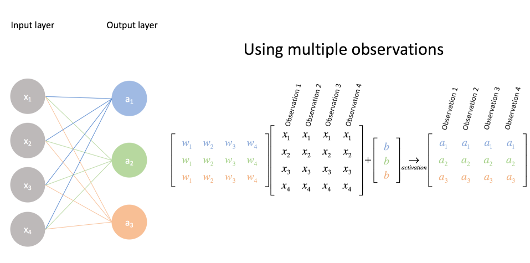
\includegraphics[width=1\linewidth]{assets/dl-mt.png}
    \caption{Nơ-ron netword và phép nhân ma trận}
    \label{fig:enter-label}
\end{figure}

\subsection{Tổng quan về các loại chip AI}
\begin{enumerate}
    \item Chip AI dựa trên ASIC (Application-Specific Integrated Circuit - Mạch tích hợp chuyên dụng)
    Đặc điểm chính:
    \begin{itemize}
        \item Được thiết kế dành riêng cho các tác vụ AI cụ thể.
        \item Hiệu năng và hiệu suất năng lượng cao nhất.
        \item Độ linh hoạt hạn chế.
    \end{itemize}
    Ví dụ: Google TPU, Tesla FSD Chip, Huawei Ascend.
    \item Chip AI dựa trên FPGA (Field-Programmable Gate Array - Mảng cổng logic lập trình được)
    Đặc điểm chính:
    \begin{itemize}
        \item Cấu trúc phần cứng có thể lập trình.
        \item Linh hoạt cao, phù hợp cho nhiều tác vụ AI khác nhau.
        \item Hiệu năng thấp hơn ASIC.
    \end{itemize}
    Ví dụ: Xilinx Alveo, Intel FPGA for AI, Microsoft Project Brainwave.
    \item Chip AI dựa trên GPU (Graphics Processing Unit - Bộ xử lý đồ họa)
    Đặc điểm chính:
    \begin{itemize}
        \item Khả năng xử lý song song mạnh mẽ.
        \item Thích hợp cho việc huấn luyện mạng nơ-ron sâu.
        \item Tiêu thụ năng lượng cao.
    \end{itemize}
    Ví dụ: Nvidia Tesla, Nvidia A100, AMD Radeon Instinct.
\end{enumerate}

\section{Bối cảnh}
\subsection{Xu hướng toàn cầu}
Trong thập kỷ qua, trí tuệ nhân tạo (AI) đã trở thành một động lực cốt lõi thúc đẩy đổi mới công nghệ trên toàn thế giới. Sự bùng nổ của các ứng dụng AI — từ nhận dạng hình ảnh, xử lý ngôn ngữ tự nhiên đến xe tự hành và phân tích dữ liệu lớn — đã kéo theo nhu cầu ngày càng cao đối với các loại chip chuyên dụng có khả năng xử lý khối lượng tính toán lớn với tốc độ cao và tiêu thụ năng lượng thấp. Đây chính là lý do AI Chips, hay còn gọi là bộ xử lý chuyên dụng cho AI, đang trở thành một lĩnh vực chiến lược trong ngành bán dẫn toàn cầu.
Các tập đoàn công nghệ hàng đầu như Google (với TPU - Tensor Processing Unit), Nvidia (với GPU hiệu năng cao), Intel và Huawei đang dẫn đầu cuộc đua phát triển AI Chips thế hệ mới. Những nỗ lực này không chỉ tập trung vào việc tăng tốc độ xử lý mà còn hướng tới tối ưu hóa hiệu suất năng lượng, mở rộng khả năng đa nhiệm và tích hợp linh hoạt vào các hệ thống AI phức tạp. Việc đầu tư mạnh mẽ vào R\&D, hợp tác với các viện nghiên cứu hàng đầu và chiến lược sở hữu trí tuệ đang giúp các công ty này thiết lập vị thế thống lĩnh trên thị trường.
Theo các báo cáo phân tích thị trường, quy mô thị trường AI Chips toàn cầu được dự đoán sẽ đạt mức hàng chục tỷ USD trong những năm tới, với tốc độ tăng trưởng kép (CAGR) vượt mức 30\%/năm. Điều này cho thấy vai trò trung tâm của AI Chips trong việc hiện thực hóa các giải pháp AI hiệu quả, nhanh chóng và linh hoạt hơn trong mọi lĩnh vực từ y tế, tài chính, an ninh quốc phòng đến các thiết bị điện tử tiêu dùng.
\subsection{Tình hình tại Việt Nam}
Tại Việt Nam, công nghệ AI vẫn đang trong giai đoạn phát triển ban đầu, tuy nhiên AI Chips đã bắt đầu nhận được sự quan tâm lớn từ cả khu vực nhà nước lẫn tư nhân. Nhận thức rõ rằng việc làm chủ phần cứng AI là yếu tố sống còn để không phụ thuộc vào các nền tảng nước ngoài, Việt Nam đang có những bước đi chiến lược để xây dựng năng lực nội tại trong lĩnh vực này.
Các tập đoàn công nghệ lớn như VinGroup (qua đơn vị VinAI) và Viettel đã đầu tư vào nghiên cứu AI Chips phục vụ cho các ứng dụng trong giám sát an ninh, giao thông thông minh, y tế và nhiều lĩnh vực khác. Đáng chú ý, các dự án phát triển chip AI nội địa đã không chỉ dừng lại ở mức nghiên cứu mà còn bước đầu thử nghiệm ứng dụng thực tiễn, đánh dấu cột mốc quan trọng cho ngành công nghệ phần cứng tại Việt Nam.
Ngoài các doanh nghiệp lớn, các trường đại học, viện nghiên cứu như Đại học Bách Khoa Hà Nội, Viện Hàn lâm Khoa học và Công nghệ Việt Nam cũng tích cực hợp tác với doanh nghiệp để đào tạo nguồn nhân lực chuyên sâu và tiến hành nghiên cứu phát triển chip AI theo hướng tối ưu chi phí, phục vụ nhu cầu đặc thù trong nước.
Mặc dù còn đối mặt với nhiều thách thức về cơ sở hạ tầng, nguồn lực và kinh nghiệm, nhưng những tín hiệu tích cực từ cả chính phủ lẫn khối tư nhân cho thấy Việt Nam đang từng bước đặt nền móng để tham gia sâu hơn vào chuỗi giá trị AI toàn cầu. Nếu duy trì được tốc độ phát triển này, Việt Nam hoàn toàn có khả năng hình thành một hệ sinh thái AI Chip nội địa có năng lực cạnh tranh khu vực trong vòng 5–10 năm tới.

\subsection{Cơ hội và thách thức trong bối cảnh Việt Nam hiện tại:}
\subsubsection{Cơ hội}
\paragraph{Nhu cầu nội địa đang mở rộng}\leavevmode\\
Sự phát triển nhanh của các lĩnh vực như thành phố thông minh, giao thông thông minh, y tế số và giáo dục số tại Việt Nam kéo theo nhu cầu lớn về các giải pháp AI tích hợp – trong đó phần cứng (AI Chips) là nền tảng cốt lõi. Đây là cơ hội để phát triển các loại chip "may đo" cho thị trường trong nước, phục vụ các nhu cầu đặc thù mà các giải pháp nước ngoài không tùy biến được.
\paragraph{Chính sách hỗ trợ từ Nhà nước}\leavevmode\\
Chính phủ Việt Nam đã xác định AI là lĩnh vực ưu tiên chiến lược. Các chương trình như “Chiến lược quốc gia về nghiên cứu, phát triển và ứng dụng AI đến năm 2030” mở ra khung pháp lý và tài chính thuận lợi cho doanh nghiệp và viện nghiên cứu đầu tư vào AI, trong đó có phần cứng.
\paragraph{Sự vào cuộc của doanh nghiệp lớn}\leavevmode\\
VinAI, Viettel, FPT, BKAV... đều đã bắt đầu hoặc công bố chiến lược nghiên cứu phát triển AI Chip. Những doanh nghiệp này có tiềm lực tài chính, đội ngũ R\&D và mối liên kết với các trường đại học lớn – tạo ra hệ sinh thái bước đầu cho ngành.
\paragraph{Cơ hội vươn ra khu vực}\leavevmode\\
Với chi phí nhân công và R\&D thấp hơn nhiều so với các nước phát triển, Việt Nam có khả năng trở thành điểm đến gia công hoặc thậm chí đồng phát triển AI Chips với các đối tác toàn cầu. Đây cũng là cơ hội để học hỏi và rút ngắn khoảng cách công nghệ.
\subsubsection{Thách thức}
\paragraph{Hạn chế về năng lực thiết kế và sản xuất}\leavevmode\\
Ngành công nghiệp bán dẫn tại Việt Nam vẫn còn non trẻ. Việt Nam chưa có nhà máy sản xuất chip ở cấp độ tiến trình hiện đại (7nm trở xuống), cũng chưa hình thành hệ thống thiết kế phần cứng quy mô lớn. Phần lớn năng lực hiện tại vẫn tập trung vào gia công lắp ráp, không phải R\&D lõi.
\paragraph{Thiếu hụt nhân lực chất lượng cao} 
Phát triển AI Chip đòi hỏi đội ngũ kỹ sư hiểu sâu về cả phần mềm AI lẫn phần cứng vi mạch – một nguồn lực rất hiếm. Các trường đại học chưa đào tạo bài bản về thiết kế chip AI, trong khi doanh nghiệp lại khó giữ chân nhân tài do cạnh tranh toàn cầu.
\paragraph{Cạnh tranh khốc liệt từ bên ngoài}\leavevmode\\
Các “ông lớn” như Nvidia, AMD, Qualcomm… đã chiếm lĩnh gần như toàn bộ thị phần AI Chips toàn cầu. Việc cạnh tranh về công nghệ, giá cả và uy tín thương hiệu với họ là một thách thức rất lớn với các công ty Việt Nam mới bắt đầu.
\paragraph{Vấn đề sở hữu trí tuệ và chuỗi cung ứng}\leavevmode\\
Phát triển chip AI không chỉ là vấn đề công nghệ mà còn liên quan đến bản quyền, giấy phép thiết kế, công cụ EDA, chuỗi cung ứng vật liệu – những thứ Việt Nam hiện vẫn phải phụ thuộc hoàn toàn vào bên ngoài. Đây là điểm yếu dễ bị tổn thương trước các rủi ro địa chính trị.
%%%%%%%%%%%%%%%%%%%%%%%%%%%%%%%%%
\section{Cơ sở lý thuyết}
\subsection{Vector Processing}
\subsubsection{SIMD - Single Instruction, Multiple Data}
SIMD là một mô hình tính toán song song thuộc phân loại Flynn (Flynn's Taxonomy), được sử dụng để thực hiện cùng một lệnh (instruction) trên nhiều phần tử dữ liệu (data) cùng lúc. Cụ thể:
\begin{itemize}
\item \textbf{Single Instruction}: Một lệnh duy nhất được phát ra.
\item \textbf{Multiple Data}: Lệnh này được áp dụng đồng thời trên nhiều phần tử dữ liệu khác nhau.
\end{itemize}
% \begin{itemize}
 
% \end{itemize}

SIMD là một dạng của \textbf{data-level parallelism} (tính song song ở cấp độ dữ liệu), nghĩa là nó khai thác tính song song bằng cách xử lý nhiều phần tử dữ liệu cùng lúc, thay vì thực hiện nhiều lệnh khác nhau (như trong mô hình MIMD - Multiple Instruction, Multiple Data).
\begin{figure}[H]
     \centering
     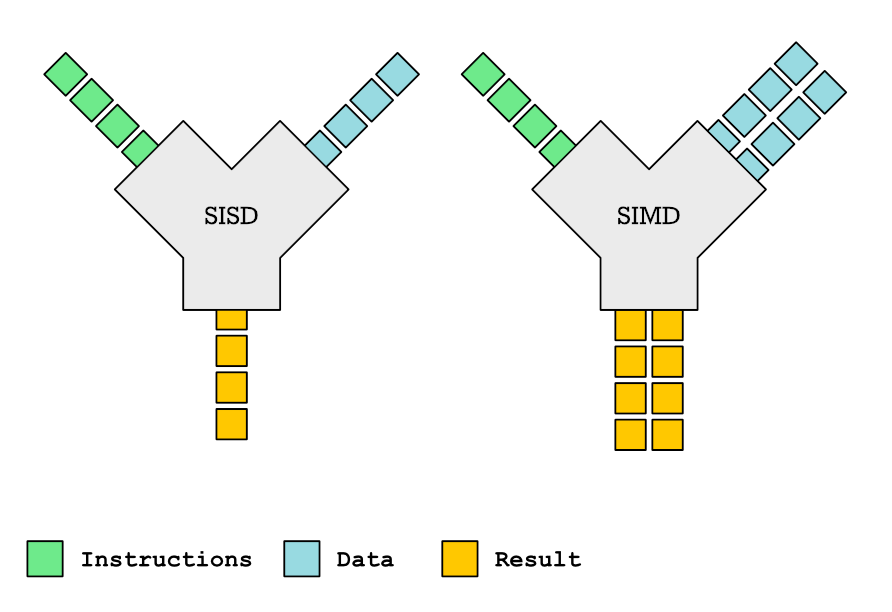
\includegraphics[scale=0.3]{assets/simd.png}
     \caption{SISD và SIMD}
     \label{fig:2ss}
 \end{figure}
 
\subsubsection{Vector Programming Model}
\paragraph{Tổng quan về Vector Programming Model} \leavevmode\\

Mô hình lập trình vector là cách mà các lập trình viên hoặc trình biên dịch tương tác với phần cứng của một máy vector. Nó cung cấp một tập hợp các tài nguyên (như thanh ghi vector) và lệnh (như lệnh vector arithmetic) để thực hiện các phép tính song song trên nhiều phần tử dữ liệu cùng lúc (theo kiểu SIMD - Single Instruction, Multiple Data). Mô hình này được thiết kế để:

\begin{itemize}
\item Tận dụng tính song song ở cấp độ dữ liệu (data-level parallelism).
\item Giảm chi phí điều khiển (control overhead) so với các mô hình scalar truyền thống.
\item Hỗ trợ các ứng dụng yêu cầu xử lý dữ liệu lớn, như tính toán khoa học, xử lý đồ họa, hoặc học máy.
\end{itemize}

\begin{figure}[H]
     \centering
     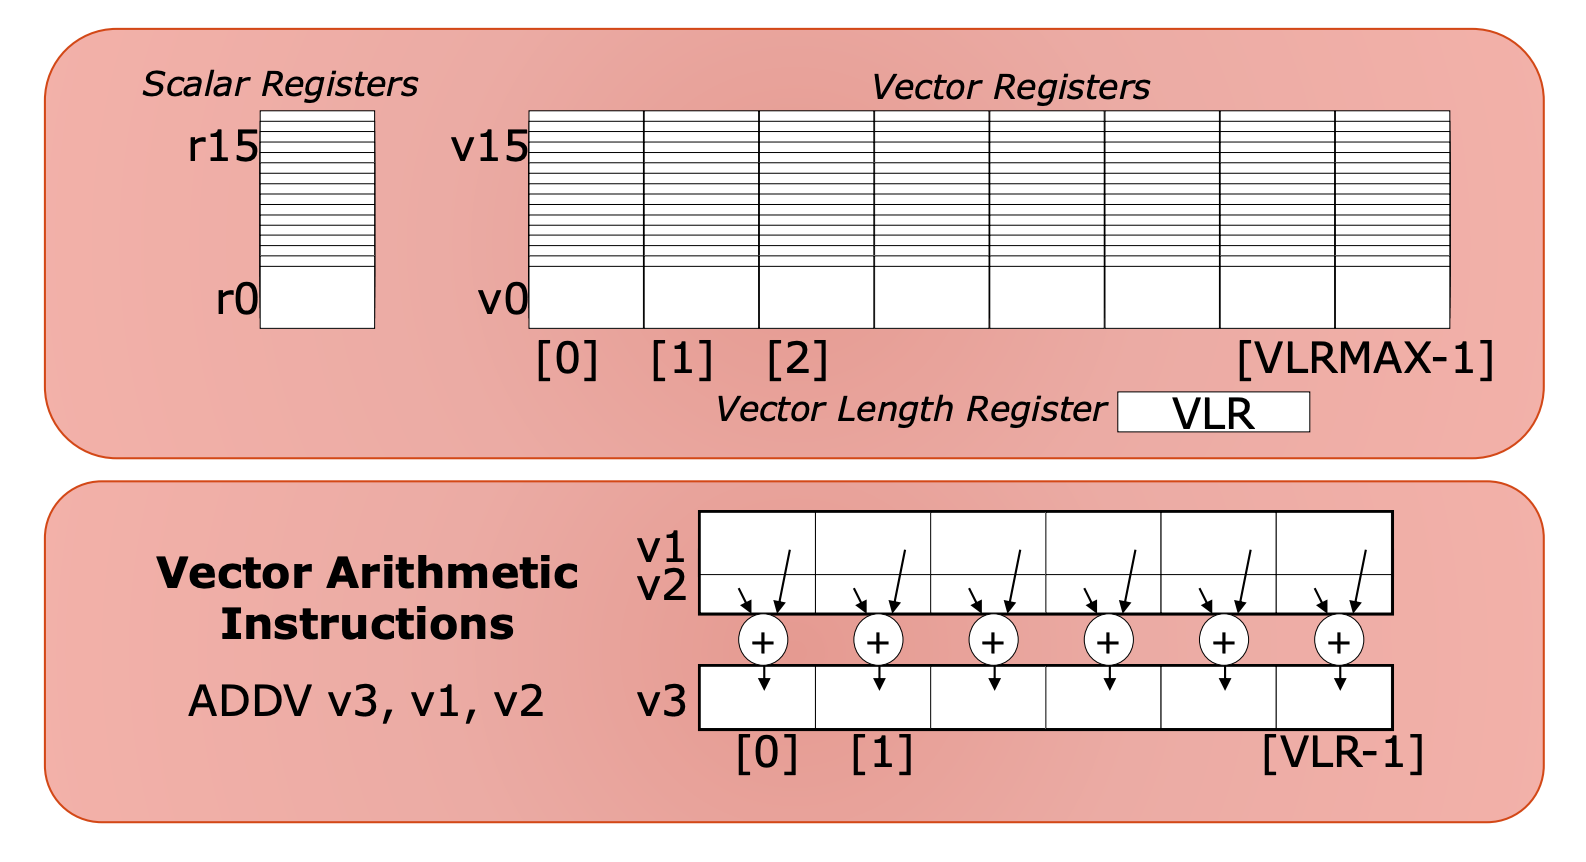
\includegraphics[scale =0.4]{assets/vector-programming-model.png}
     \caption{Vector programming model}
     \label{fig:2ss}
 \end{figure}

 Hình ảnh thể hiện một phần của kiến trúc lập trình vector, một mô hình được thiết kế để xử lý dữ liệu dạng mảng (vector) một cách hiệu quả. Cụ thể, nó bao gồm các thanh ghi scalar (r0 đến r15) dùng để lưu trữ các giá trị đơn lẻ như địa chỉ hay hằng số, và các thanh ghi vector (v0 đến v15) dùng để chứa các tập hợp dữ liệu lớn hơn, tức là các vector. Ngoài ra, còn có VLR, một thanh ghi đặc biệt quyết định số phần tử của vector sẽ được xử lý trong mỗi lệnh, và một ví dụ về lệnh vector là ADDV, thực hiện phép cộng giữa các vector. Tất cả các thành phần này phối hợp để tạo nên một hệ thống xử lý dữ liệu song song mạnh mẽ.

\paragraph{Thanh ghi Scalar (Scalar Registers)}\leavevmode\\

Thanh ghi scalar, được ký hiệu từ r0 đến r15 trong hình (tổng cộng 16 thanh ghi), là những thanh ghi thông thường mà ta thường thấy trong các kiến trúc máy tính cơ bản. Mỗi thanh ghi này chỉ lưu trữ được một giá trị đơn, gọi là giá trị scalar, chẳng hạn như một số nguyên hoặc một địa chỉ bộ nhớ. Chúng đóng vai trò như những "trợ thủ" trong việc điều khiển và hỗ trợ các phép tính vector. Ví dụ, r0 có thể chứa địa chỉ bắt đầu của một vector trong bộ nhớ, còn r1 có thể lưu giá trị stride, tức là khoảng cách giữa các phần tử liên tiếp trong vector đó. Nhờ tính đơn giản và linh hoạt, các thanh ghi scalar thường được dùng để quản lý vòng lặp, lưu trữ hằng số hoặc cung cấp thông tin đầu vào cho các lệnh vector, giúp quá trình xử lý dữ liệu trơn tru hơn.

\paragraph{Thanh ghi Vector (Vector Registers)}\leavevmode\\

Khác với thanh ghi scalar, các thanh ghi vector (v0 đến v15, cũng có 16 thanh ghi trong hình) được thiết kế đặc biệt để lưu trữ toàn bộ một vector, tức là một dãy các phần tử dữ liệu. Mỗi thanh ghi vector có thể chứa nhiều giá trị, từ phần tử đầu tiên [0] cho đến phần tử cuối cùng [VLRMAX-1], trong đó VLRMAX là độ dài tối đa mà phần cứng cho phép, ví dụ như 64 phần tử. Điều này có nghĩa là nếu VLRMAX là 64, thì một thanh ghi như v1 có thể chứa một dãy dữ liệu như [a0, a1, ..., a63], và v2 chứa [b0, b1, ..., b63]. Công dụng chính của chúng là lưu trữ dữ liệu để thực hiện các phép tính song song, cho phép máy tính xử lý nhiều phần tử cùng lúc thay vì từng phần tử một như cách truyền thống. Đây chính là điểm mạnh của lập trình vector, giúp tăng tốc độ xử lý đáng kể.

\paragraph{Thanh ghi Độ dài Vector (Vector Length Register - VLR)}\leavevmode\\

VLR là một thanh ghi đặc biệt, đóng vai trò như "người điều phối" trong mô hình lập trình vector. Nó lưu trữ độ dài hiện tại của vector mà các lệnh vector sẽ xử lý, với giá trị nằm trong khoảng từ 1 đến VLRMAX. Ví dụ, nếu VLR được đặt là 32, thì máy chỉ xử lý 32 phần tử đầu tiên của thanh ghi vector (từ [0] đến [31]), bỏ qua các phần tử còn lại dù thanh ghi có thể chứa tối đa 64 phần tử. Điều này mang lại sự linh hoạt lớn: không phải vector nào cũng cần xử lý hết độ dài tối đa, và VLR giúp máy thích nghi với các kích thước vector khác nhau mà không cần phải thêm dữ liệu giả (padding) để lấp đầy. Trong lập trình, khi một vòng lặp lớn được chia thành các đoạn nhỏ để vector hóa, VLR đặc biệt hữu ích ở đoạn cuối – nơi số phần tử còn lại thường nhỏ hơn VLRMAX. Chẳng hạn, nếu chỉ còn 10 phần tử cần xử lý, VLR được đặt thành 10 để đảm bảo xử lý đúng và đủ.

\paragraph{Lệnh Số học Vector (Vector Arithmetic Instructions)}\leavevmode\\

\begin{figure}[H]
    \centering
    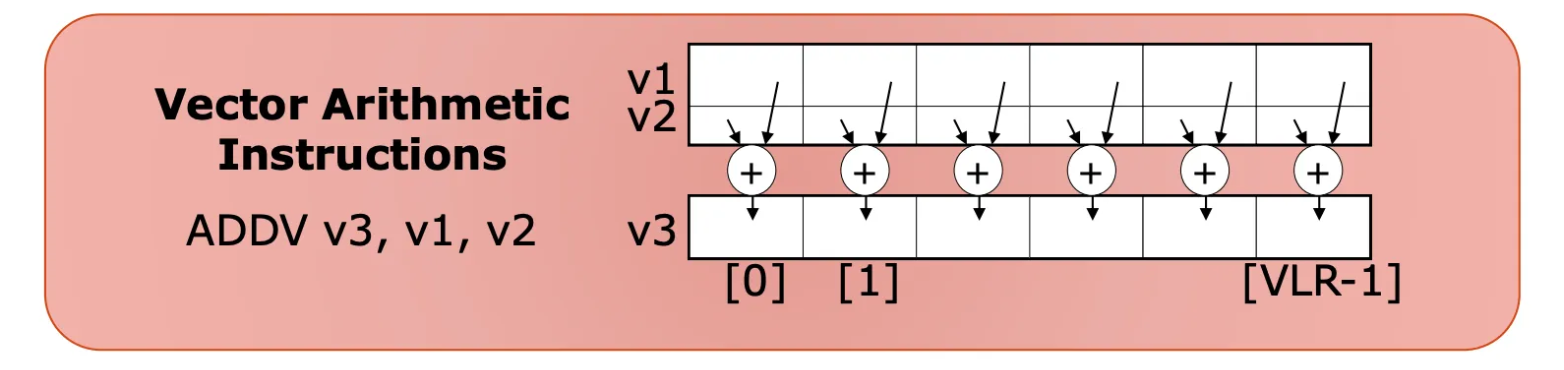
\includegraphics[width=1\linewidth]{assets/vector-arithmetic-instructions.png}
    \caption{Minh họa lệnh số học vector}
    \label{fig:enter-label}
\end{figure}

Hình bên trên minh họa một lệnh cụ thể là ADDV v3, v1, v2, trong đó:

\begin{itemize}
    \item \textbf{ADDV} là lệnh cộng vector
    \item \textbf{v1} và \textbf{v2} là hai vector đầu vào 
    \item \textbf{v3} là vector kết quả
\end{itemize}
Cách lệnh này hoạt động khá đơn giản nhưng hiệu quả: nó lấy từng cặp phần tử tương ứng từ \textbf{v1} và \textbf{v2}, cộng chúng lại và ghi kết quả vào \textbf{v3}. Cụ thể, với mỗi chỉ số i, \textbf{v3[i] = v1[i] + v2[i]}. Tuy nhiên, số phần tử được xử lý không phải lúc nào cũng là toàn bộ vector mà phụ thuộc vào giá trị của \textbf{VLR}. Nếu VLR = 32, lệnh sẽ thực hiện 32 phép cộng, cụ thể:
\begin{itemize}
    \item v3[0] = v1[0] + v2[0]
    \item v3[1] = v1[1] + v2[1]
    \item ...
    \item v3[30] = v1[30] + v2[30]
    \item v3[31] = v1[31] + v2[31]
\end{itemize}
các phần tử còn lại (từ [32] đến [63] nếu VLRMAX = 64) sẽ không bị ảnh hưởng.
\subsubsection{Vector Stripming}
Thanh ghi vector trong máy vector có kích thước cố định, ví dụ 64 phần tử. Nếu một vòng lặp cần xử lý nhiều hơn số phần tử mà thanh ghi vector có thể chứa (ví dụ: 1000 phần tử), ta không thể xử lý toàn bộ vòng lặp trong một lần thực thi lệnh vector. Kỹ thuật \textbf{stripming} chia vòng lặp lớn thành các đoạn nhỏ (strips) có kích thước vừa với thanh ghi vector (ví dụ: 64 phần tử mỗi đoạn). Mỗi đoạn được xử lý bằng lệnh vector, sau đó lặp lại cho đến khi toàn bộ vòng lặp hoàn tất.
\begin{multicols}{2}
\begin{figure}[H]
    \centering
    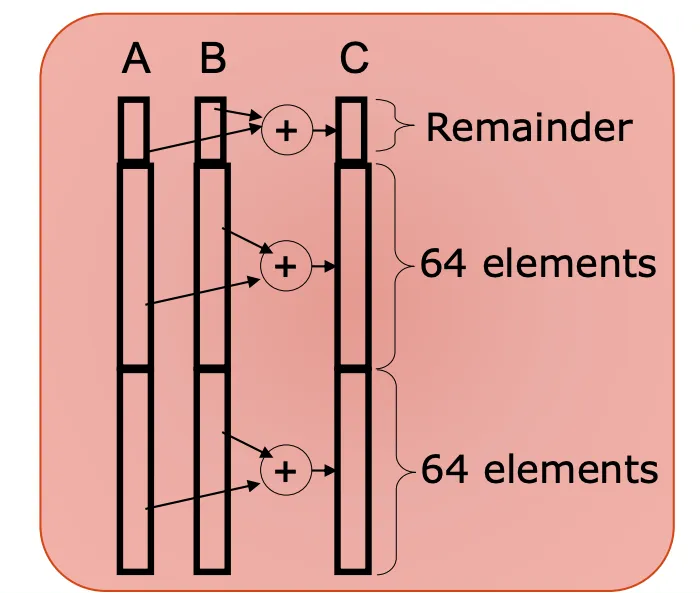
\includegraphics[width=1\linewidth]{assets/vector-stripming.png}
    \caption{Vector stripming}
    \label{fig:enter-label}
\end{figure}
\columnbreak
\textbf{Minh họa Stripming: Vector A, B, C}: Ba cột đại diện cho mảng A, B, và C. Mỗi cột được chia thành các đoạn (strips) 64 phần tử (được đánh dấu là "64 elements"). Phần còn lại (remainder) là số phần tử không đủ để tạo thành một đoạn 64 phần tử (ví dụ: nếu N = 1000, thì sau 15 đoạn 64 phần tử, còn lại 40 phần tử).

\textbf{Quá trình thực thi}: Mỗi đoạn 64 phần tử được xử lý bằng lệnh vector:
\begin{itemize}
    \item Lấy 64 phần tử từ A và B.
    \item Thực hiện phép cộng A[i] + B[i].
    \item Lưu kết quả vào 64 phần tử tương ứng của C.
\end{itemize}
Sau khi xử lý một đoạn, con trỏ của A, B, và C được cập nhật để trỏ đến đoạn tiếp theo. Quá trình lặp lại cho đến khi xử lý hết các đoạn đầy đủ, sau đó xử lý phần remainder (nếu có).
\end{multicols}

\textbf{Ý nghĩa}:
\begin{itemize}
    \item Stripming cho phép máy vector xử lý các vòng lặp lớn hơn kích thước thanh ghi vector, đảm bảo tính linh hoạt và hiệu quả.
    \item  Phần remainder (phần còn lại) sẽ được xử lý trong lần lặp cuối cùng, với độ dài vector được điều chỉnh để vừa với số phần tử còn lại.
\end{itemize}

\subsubsection{Vector Arithmetic Execution}
Phần này mô tả cách máy vector thực thi các phép toán vector (như phép nhân V3 ← V1 * V2) bằng cách sử dụng pipeline sâu. Pipeline sâu giúp tăng tần số xung nhịp và thông lượng, trong khi tính độc lập của các phép toán vector loại bỏ pipeline hazards, dẫn đến điều khiển đơn giản và hiệu suất cao. Đây là một ví dụ điển hình về cách thiết kế phần cứng (pipeline) và phần mềm (lệnh vector) phối hợp để tối ưu hóa hiệu suất, một nguyên tắc quan trọng trong khoa học máy tính và kiến trúc máy tính.

\begin{multicols}{2}
\begin{figure}[H]
    \centering
    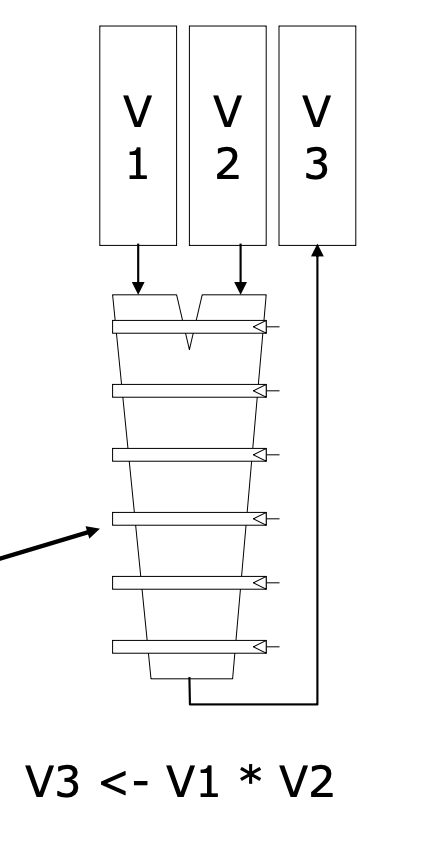
\includegraphics[width=0.7\linewidth]{assets/deep-pipeline.png}
    \caption{Deep pipeline trên 1 unit}
    \label{fig:enter-label}
\end{figure}
\columnbreak
\textbf{Các thành phần}: Ba vector V1, V2, V3:
\begin{itemize}
    \item Ba cột đại diện cho các thanh ghi vector V1, V2, và V3.
    \item V1 và V2 là các vector đầu vào, mỗi vector chứa nhiều phần tử (ví dụ: 64 phần tử nếu thanh ghi vector có kích thước 64).
    \item V3 là vector kết quả, lưu kết quả của phép nhân $V1[i] * V2[i]$ cho mỗi chỉ số i.
\end{itemize}
\textbf{Pipeline sâu}:
\begin{itemize}
    \item Được minh họa bằng một hình phễu (funnel-like structure) với nhãn "Six stage multiply pipeline" (Pipeline nhân 6 giai đoạn).
    \item Pipeline này có 6 giai đoạn (stages), nghĩa là mỗi phép nhân được chia thành 6 bước nhỏ, mỗi bước được thực hiện trong một chu kỳ xung nhịp.
\end{itemize}
\end{multicols}
\paragraph{Đặc điểm}\leavevmode\\
Thực thi phép toán vector có các đặc điểm quan trọng như sau:
\begin{enumerate}
    \item \textbf{Deep pipeline → Fast clock!}\par Trong một pipeline sâu, mỗi giai đoạn chỉ thực hiện một phần nhỏ của phép toán, nên thời gian cho mỗi giai đoạn ngắn hơn. Điều này cho phép tăng tần số xung nhịp (clock frequency), vì tần số xung nhịp tỷ lệ nghịch với thời gian của giai đoạn dài nhất.\par
    Ví dụ: Nếu một phép nhân mất 6 ns mà không có pipeline, thì tần số tối đa là 1/6ns = 166 MHz. Nhưng nếu chia thành 6 giai đoạn, mỗi giai đoạn mất 1 ns, tần số có thể tăng lên 1/1ns = 1 GHz.	Tần số cao hơn giúp máy vector xử lý nhanh hơn, đặc biệt với các tác vụ tính toán lớn.

    \item \textbf{Much simpler pipeline control}	\par Trong các CPU thông thường (scalar), pipeline phải xử lý các lệnh khác nhau (như cộng, nhân, load, store), dẫn đến các vấn đề phức tạp như xung đột lệnh (control hazards) hoặc xung đột dữ liệu (data hazards). \par
    Trong máy vector, các lệnh vector (như VADD, VMUL) áp dụng cùng một phép toán cho nhiều phần tử, nên điều khiển pipeline đơn giản hơn. Không cần kiểm tra phụ thuộc giữa các phần tử, vì chúng độc lập.	Điều khiển đơn giản giảm chi phí phần cứng và tăng độ tin cậy của hệ thống.

    \item \textbf{Operations are independent → no pipeline hazards}. \par Pipeline hazards là các vấn đề làm gián đoạn luồng xử lý trong pipeline, bao gồm:
    \begin{itemize}
        \item Data hazards: Xung đột dữ liệu (ví dụ: một lệnh cần kết quả của lệnh trước đó).
        \item Control hazards: Xung đột điều khiển (ví dụ: do nhánh điều kiện).
        \item Structural hazards: Xung đột tài nguyên (ví dụ: hai lệnh cần cùng một đơn vị chức năng).
    \end{itemize}
    Trong máy vector, các phép toán trên từng phần tử vector là độc lập (ví dụ: V1[0] * V2[0] không phụ thuộc vào V1[1] * V2[1]). Do đó, không có data hazards giữa các phần tử trong cùng một lệnh vector. Tính độc lập này loại bỏ pipeline hazards, cho phép đường ống xử lý hoạt động liên tục và đạt thông lượng tối đa. Điều này làm cho máy vector trở thành một kiến trúc hiệu quả cho các ứng dụng có tính song song dữ liệu cao, và cũng là một ý tưởng quan trọng khi thiết kế các hệ thống tính toán song song trên FPGA trong Reconfigurable Computing.

    \item \textbf{Vector maximizes advantages of pipelining and avoids its downsides} \par \textbf{Lợi ích của pipelining}: Tăng thông lượng bằng cách xử lý nhiều phần tử cùng lúc ở các giai đoạn khác nhau.
    
    \textbf{Nhược điểm của pipelining}: Trong các hệ thống scalar, pipeline hazards có thể làm giảm hiệu suất (ví dụ: phải dừng pipeline để chờ dữ liệu hoặc xử lý nhánh).
    Máy vector tận dụng tính độc lập của các phép toán vector để tránh các nhược điểm này, đồng thời khai thác tối đa lợi ích của pipelining.	Máy vector là một ví dụ điển hình về việc thiết kế phần cứng và phần mềm phối hợp để đạt hiệu suất cao.
\end{enumerate}

\subsubsection{Vector Instruction Execution}
\paragraph{Tổng quan về Vector Instruction Execution}\leavevmode\\

Cách một máy vector thực thi một lệnh vector, cụ thể là lệnh ADDV C, A, B (cộng vector) như thế nào? Lệnh này có nghĩa là: lấy các phần tử của vector A cộng với các phần tử tương ứng của vector B, rồi lưu kết quả vào vector C.

Điểm đặc biệt ở đây là máy vector có khả năng \textbf{microarchitecturally vary the number of \textit{lanes}} (thay đổi số lượng "lanes" ở cấp độ vi kiến trúc). \textbf{Lanes} ở đây có thể hiểu là các đơn vị chức năng song song (functional units) mà máy sử dụng để thực thi lệnh vector. Hình ảnh so sánh hai cách thực thi:
\begin{itemize}
    \item \textbf{Bên trái}: Sử dụng một đơn vị chức năng (one pipelined functional unit).
    \item \textbf{Bên phải}: Sử dụng bốn đơn vị chức năng song song (four pipelined functional units).
\end{itemize}

\begin{figure}[H]
    \centering
    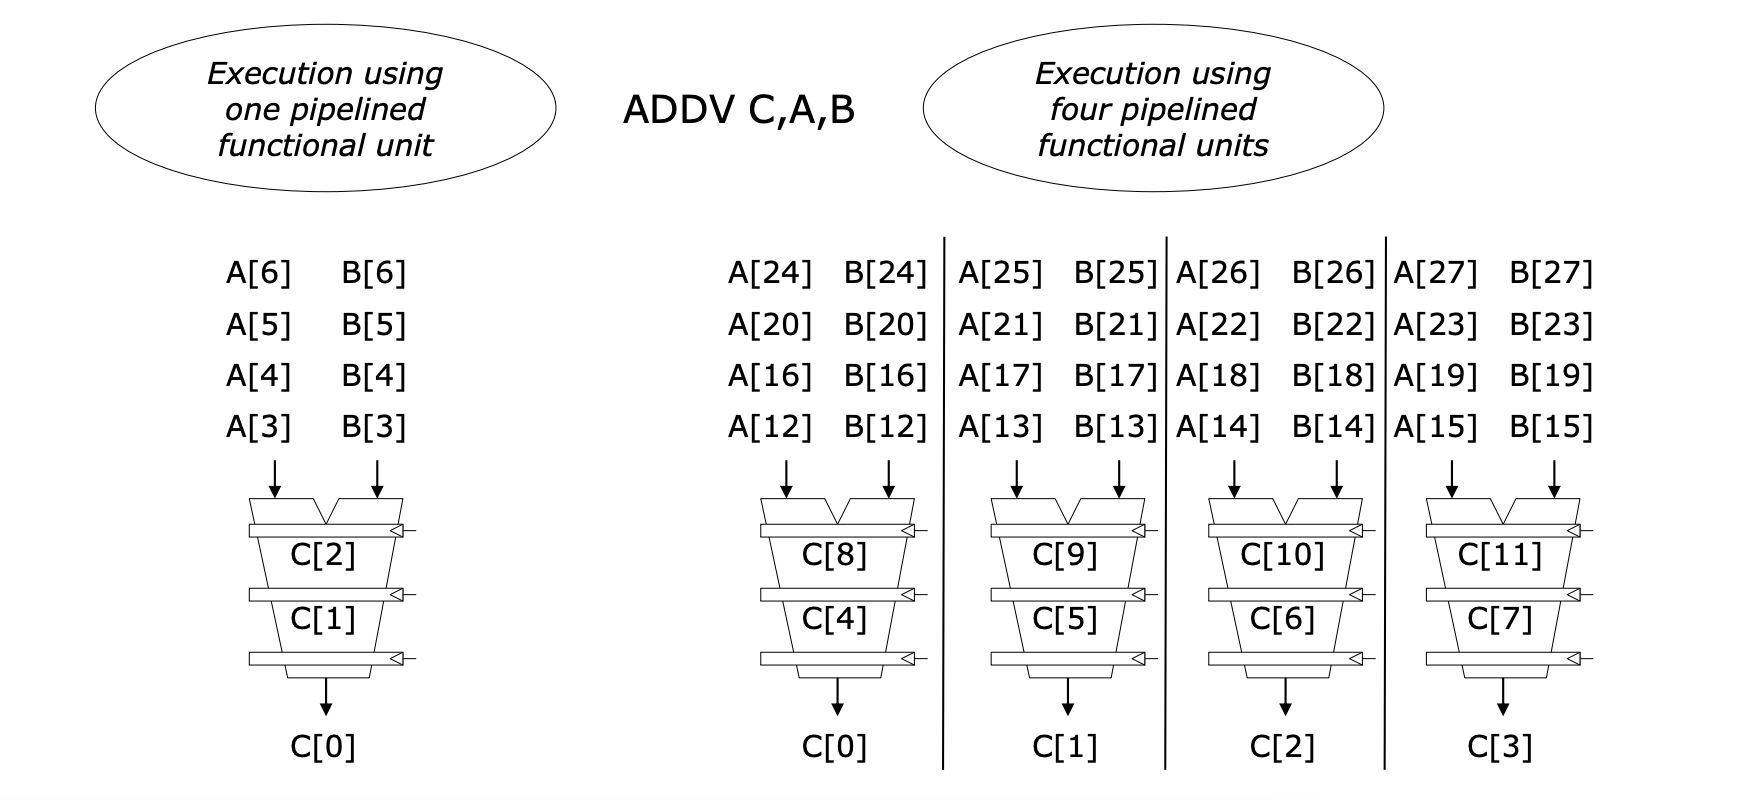
\includegraphics[width=1\linewidth]{assets/vector-instruction-execution.png}
    \caption{Vector instruction execution}
    \label{fig:enter-label}
\end{figure}

\paragraph{Thực thi}\leavevmode\\

\textbf{Các thành phần trong hình}
\begin{itemize}
    \item \textbf{A[i], B[i], C[i]}: Đây là các vector, với mỗi phần tử được đánh chỉ số (index). Ví dụ: \par
    \begin{itemize}
        \item A[6] là phần tử thứ 6 của vector A.
        \item B[6] là phần tử thứ 6 của vector B.
        \item C[2] là phần tử thứ 2 của vector C.
    \end{itemize}
    \item \textbf{ADDV C, A, B}: Lệnh vector yêu cầu thực hiện phép cộng: \textbf{C[i] = A[i] + B[i]} cho tất cả các phần tử i trong vector.
    \item Pipelined Functional Unit: Đây là các đơn vị chức năng được tổ chức theo dạng pipeline (dây chuyền). Pipeline cho phép xử lý nhiều phép tính liên tiếp mà không cần chờ phép tính trước hoàn thành, giúp tăng hiệu suất.
\end{itemize}
\newpage
\textbf{Thực thi với một đơn vị chức năng (one pipelined functional unit)}
\begin{multicols}{2}
\begin{figure}[H]
    \centering
    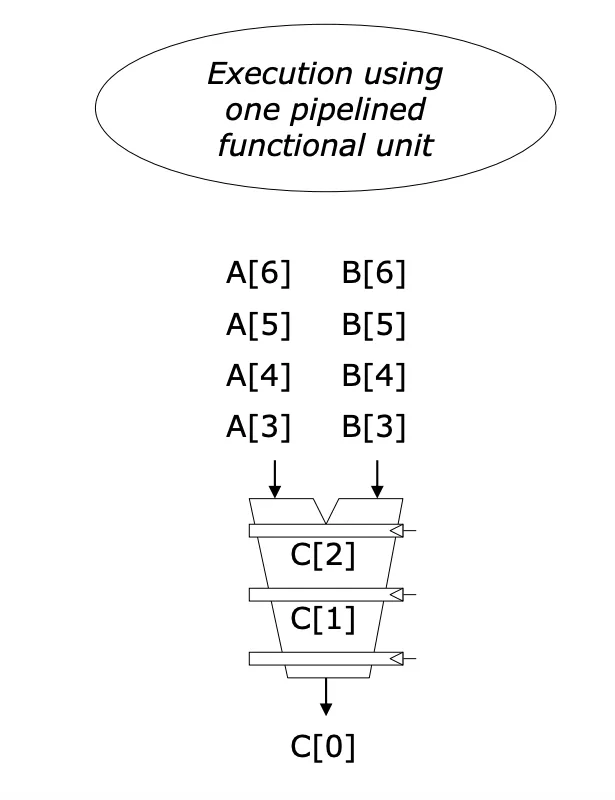
\includegraphics[width=1\linewidth]{assets/vector-execution-1.png}
    \caption{Vector execution with 1 unit}
    \label{fig:enter-label}
\end{figure}
\columnbreak
\textbf{Cách hoạt động}:
\begin{itemize}
    \item Máy chỉ có \textbf{một đơn vị chức năng} để thực hiện phép cộng.
    \item Các phần tử của vector A và B được xử lý \textbf{tuần tự} qua đơn vị chức năng này.
\end{itemize}
Ví dụ:
\begin{itemize}
    \item Đầu tiên, A[6] và B[6] được cộng để tạo ra C[2].
    \item Tiếp theo, A[5] và B[5] được cộng để tạo ra C[1].
    \item Cứ tiếp tục như vậy cho đến A[3] và B[3] để tạo ra C[0].
    \item Kết quả được ghi lần lượt vào C[2], C[1], C[0].
\end{itemize}
\textbf{Hiệu suất}:
\begin{itemize}
    \item Vì chỉ có một đơn vị chức năng, các phép tính được thực hiện \textbf{tuần tự} qua pipeline.
    \item Điều này có nghĩa là thời gian thực thi tỷ lệ thuận với độ dài của vector (ở đây là 3 phần tử, nên cần 3 chu kỳ chính để hoàn thành, cộng thêm độ trễ của pipeline).
\end{itemize}
\end{multicols}

\textbf{Thực thi với bốn đơn vị chức năng (four pipelined functional units)}

\begin{multicols}{2}
\begin{figure}[H]
    \centering
    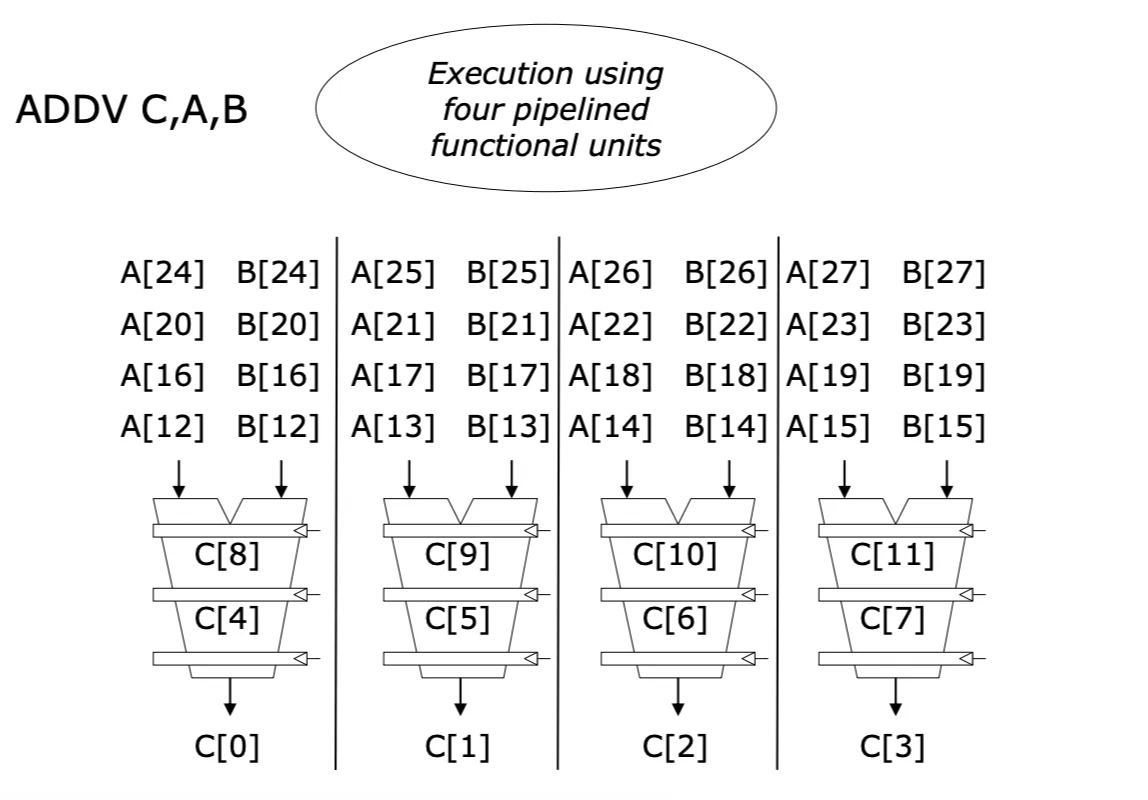
\includegraphics[width=1\linewidth]{assets/vector-execution-2.png}
    \caption{Vector execution with 4 unit}
    \label{fig:enter-label}
\end{figure}
\columnbreak
\textbf{Cách hoạt động}:
\begin{itemize}
    \item Máy có \textbf{bốn đơn vị chức năng} hoạt động song song (gọi là 4 lanes).
    \item Các phần tử của vector A và B được chia thành các nhóm và xử lý song song trên 4 lanes này.
\end{itemize}
Ví dụ:
\begin{itemize}
    \item Lane 1: Xử lý A[24] + B[24] → C[8], sau đó A[20] + B[20] → C[4], v.v.
    \item Lane 2: Xử lý A[25] + B[25] → C[9], sau đó A[21] + B[21] → C[5], v.v.
    \item Lane 3: Xử lý A[26] + B[26] → C[10], sau đó A[22] + B[22] → C[6], v.v.
    \item Lane 4: Xử lý A[27] + B[27] → C[11], sau đó A[23] + B[23] → C[7], v.v.
    \item Kết quả được ghi song song vào C[8] đến C[11], sau đó C[4] đến C[7], v.v.
\end{itemize}
\textbf{Hiệu suất}:
\begin{itemize}
    \item Vì có 4 lanes, máy có thể xử lý \textbf{4 phần tử cùng lúc} trong mỗi chu kỳ.
    \item Nếu vector có 12 phần tử (như trong ví dụ), thì chỉ cần \textbf{12 / 4 = 3} chu kỳ chính (cộng thêm độ trễ pipeline) để hoàn thành, nhanh hơn nhiều so với cách bên trái.
\end{itemize}
\end{multicols}

\subsubsection{Vector Unit Structure}
\paragraph{Tổng quan về Vector Unit Structure}\leavevmode\\

Đơn vị vector là một phần của bộ xử lý chuyên dụng để thực hiện các phép tính trên nhiều phần tử dữ liệu cùng lúc (theo kiểu SIMD - Single Instruction, Multiple Data).

Các thành phần chính trong hình bao gồm:
\begin{itemize}
    \item \textbf{Functional Units} (Đơn vị chức năng): Thực hiện các phép tính (như cộng, nhân, v.v.).
    \item \textbf{Vector Registers} (Thanh ghi vector): Lưu trữ dữ liệu vector.
    \item \textbf{Lanes}: Các đường xử lý song song trong đơn vị vector.
    \item \textbf{Memory Subsystem} (Hệ thống bộ nhớ): Nơi dữ liệu được đọc/ghi từ bộ nhớ chính.
\end{itemize}

Hình ảnh cũng nhấn mạnh một nguyên tắc thiết kế quan trọng: \textit{"Registers are kept nearby functional units to minimize data movement"(Thanh ghi được đặt gần các đơn vị chức năng để giảm thiểu việc di chuyển dữ liệu)} . Đây là một yếu tố cốt lõi để tối ưu hóa hiệu suất trong các hệ thống vector.

\begin{figure}[H]
    \centering
    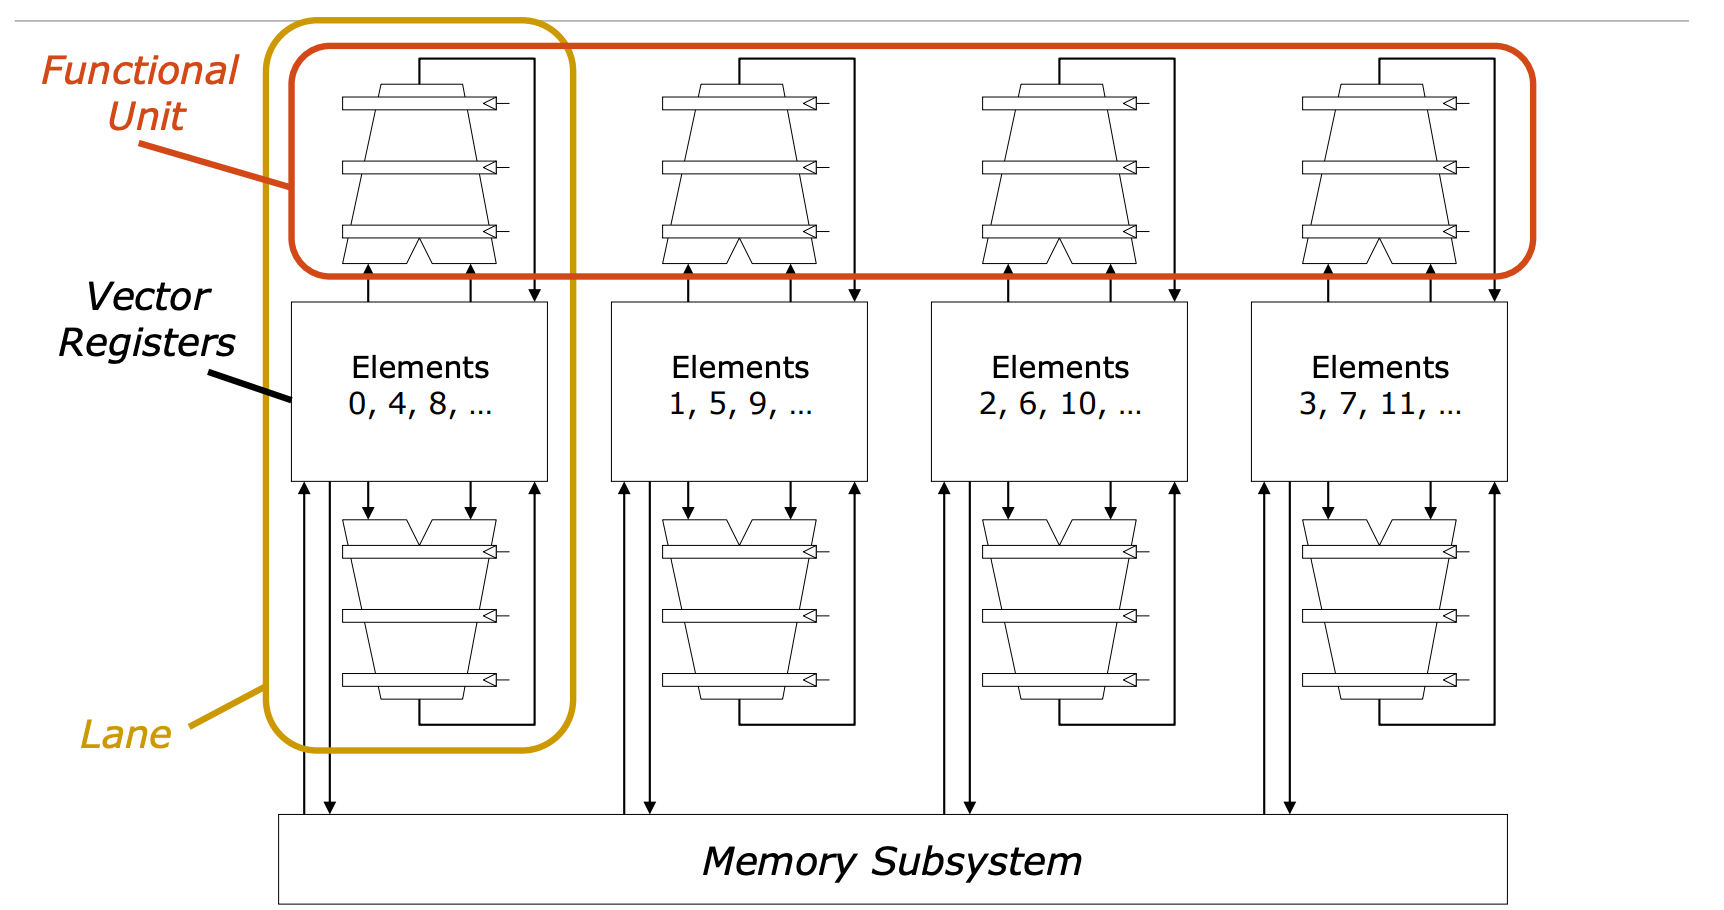
\includegraphics[width=1\linewidth]{assets/vector-unit.png}
    \caption{Vector unit structure}
    \label{fig:enter-label}
\end{figure}

\paragraph{Giải thích chi tiết các thành phần trong hình}\leavevmode\\
\begin{enumerate}
    \item Functional Units (Đơn vị chức năng)
    \begin{itemize}
        \item Được biểu diễn ở phía trên cùng của mỗi lane.
        \item Mỗi đơn vị chức năng là một khối phần cứng chuyên dụng để thực hiện các phép tính (ví dụ: phép cộng, nhân, hoặc các phép toán logic).
        \item Các đơn vị chức năng này được tổ chức theo dạng pipeline, nghĩa là chúng có thể xử lý nhiều phép tính liên tiếp mà không cần chờ phép tính trước hoàn thành. Điều này giúp tăng hiệu suất bằng cách tận dụng tính song song trong pipeline.
    \end{itemize}
    \item Vector Registers (Thanh ghi vector)
    \begin{itemize}
        \item Thanh ghi vector là nơi lưu trữ các vector (dữ liệu dạng mảng) để xử lý.
        \item Trong hình, các thanh ghi vector được chia thành 4 nhóm, mỗi nhóm chứa các phần tử của vector được phân bổ theo một cách cụ thể:
        \begin{itemize}
            \item Nhóm 1: Lưu trữ các phần tử 0, 4, 8, ...
            \item Nhóm 2: Lưu trữ các phần tử 1, 5, 9, ...
            \item Nhóm 3: Lưu trữ các phần tử 2, 6, 10, ...
            \item Nhóm 4: Lưu trữ các phần tử 3, 7, 11, ...
        \end{itemize}
        \item Cách phân bổ này được gọi là \textbf{"interleaving"} (đan xen):
        \begin{itemize}
            \item Thay vì lưu trữ các phần tử liên tiếp (0, 1, 2, 3, ...) trong cùng một thanh ghi, các phần tử được phân chia đều cho các lane.
            \item Ví dụ: Nếu vector có 12 phần tử (0 đến 11), thì lane 1 xử lý phần tử 0, 4, 8; lane 2 xử lý phần tử 1, 5, 9; v.v.
        \end{itemize}
        \item Lý do của việc đan xen:
        \begin{itemize}
            \item Đảm bảo rằng mỗi lane có thể xử lý một phần dữ liệu độc lập, tránh xung đột khi truy cập dữ liệu.
            \item Tăng tính song song: Mỗi lane có thể hoạt động độc lập trên tập dữ liệu riêng của nó.
        \end{itemize}
    \end{itemize}
    \item Lanes
    \begin{itemize}
        \item Mỗi \textbf{lane} là một đường xử lý song song, bao gồm:
        \begin{itemize}
            \item Một đơn vị chức năng (functional unit).
            \item Một tập hợp thanh ghi vector (vector registers) tương ứng.
        \end{itemize}
        \item Trong hình, có \textbf{4 lanes}, nghĩa là đơn vị vector này có thể xử lý \textbf{4 phần tử cùng lúc} trong mỗi chu kỳ.
        \item Mỗi lane hoạt động độc lập:
        \begin{itemize}
            \item Lane 1 xử lý các phần tử 0, 4, 8, ...
            \item Lane 2 xử lý các phần tử 1, 5, 9, ...
            \item Lane 3 xử lý các phần tử 2, 6, 10, ...
            \item Lane 4 xử lý các phần tử 3, 7, 11, ...
        \end{itemize}
        \item \textbf{Lợi ích của lanes}:
        \begin{itemize}
            \item \textbf{Tăng tính song song}: Với 4 lanes, đơn vị vector có thể xử lý 4 phần tử cùng lúc, giúp tăng tốc độ thực thi lên gấp 4 lần so với việc chỉ có 1 lane.
            \item \textbf{Phù hợp với các ứng dụng} cần xử lý dữ liệu lớn, như tính toán ma trận, xử lý đồ họa, hoặc học máy.
        \end{itemize}
    \end{itemize}
    \item Memory Subsystem (Hệ thống bộ nhớ)
    \begin{itemize}
        \item Nằm ở phía dưới cùng của hình, đại diện cho bộ nhớ chính (RAM) hoặc bộ nhớ cache.
        \item Dữ liệu được đọc từ bộ nhớ chính vào các thanh ghi vector để xử lý, và kết quả sau khi xử lý được ghi ngược lại vào bộ nhớ chính.
        \item Mỗi lane có một kết nối trực tiếp với hệ thống bộ nhớ, cho phép đọc/ghi dữ liệu song song. Điều này rất quan trọng để đảm bảo băng thông bộ nhớ đủ lớn, tránh tình trạng \textit{memory bottleneck} (nút cổ chai bộ nhớ).
    \end{itemize}
    
    \item Nguyên tắc thiết kế: \textit{"Registers are kept nearby functional units to minimize data movement"}
    \begin{itemize}
        \item Có nghĩa là các thanh ghi vector được đặt \textbf{gần} các đơn vị chức năng (functional units) trong mỗi lane.
        \item \textbf{Lý do}:
        \begin{itemize}
            \item \textbf{Giảm độ trễ (latency)}: Nếu thanh ghi ở xa, việc di chuyển dữ liệu từ thanh ghi đến đơn vị chức năng sẽ mất nhiều thời gian hơn.
            \item \textbf{Tăng hiệu suất}: Khi thanh ghi ở gần, dữ liệu có thể được truy cập nhanh chóng, giúp đơn vị chức năng hoạt động liên tục mà không bị gián đoạn.
            \item \textbf{Tiết kiệm năng lượng}: Di chuyển dữ liệu qua các khoảng cách dài trong chip tiêu tốn nhiều năng lượng hơn.
        \end{itemize}
        \item Đây là một nguyên tắc quan trọng trong thiết kế vi kiến trúc, đặc biệt trong các hệ thống hiệu năng cao như CPU vector hoặc GPU.
    \end{itemize}
\end{enumerate}

\paragraph{Cách hoạt động của Vector Unit}\leavevmode\\
Hãy tưởng tượng đơn vị vector này đang thực thi một lệnh như \texttt{ADDV C, A, B} (cộng vector A và B, lưu kết quả vào C):

\begin{enumerate}
    \item \textbf{Đọc dữ liệu}:
    \begin{itemize}
        \item Các phần tử của vector A và B được đọc từ bộ nhớ chính (memory subsystem) vào các thanh ghi vector.
        \item Dữ liệu được phân bổ đan xen:
        \begin{itemize}
            \item Lane 1: Nhận A[0], B[0], A[4], B[4], ...
            \item Lane 2: Nhận A[1], B[1], A[5], B[5], ...
            \item Và tương tự cho các lane còn lại.
        \end{itemize}
    \end{itemize}
    
    \item \textbf{Xử lý song song}:
    \begin{itemize}
        \item Mỗi lane thực hiện phép cộng trên các phần tử tương ứng:
        \begin{itemize}
            \item Lane 1: $C[0] = A[0] + B[0]$, sau đó $C[4] = A[4] + B[4]$, ...
            \item Lane 2: $C[1] = A[1] + B[1]$, sau đó $C[5] = A[5] + B[5]$, ...
            \item Các lane khác tương tự.
        \end{itemize}
        \item Vì có 4 lanes, 4 phép cộng được thực hiện cùng lúc trong mỗi chu kỳ.
    \end{itemize}
    
    \item \textbf{Ghi kết quả}: Kết quả ($C[0], C[1], C[2], C[3], ...$) được ghi từ các thanh ghi vector trở lại bộ nhớ chính.
\end{enumerate}

\subsubsection{Vector Memory System}
\paragraph{Tổng quan về Vector Memory System}
Hệ thống bộ nhớ vector được thiết kế để hỗ trợ các bộ xử lý vector, vốn cần truy cập một lượng lớn dữ liệu cùng lúc để thực hiện các phép toán song song (SIMD - Single Instruction, Multiple Data). Trong các hệ thống như vậy, băng thông bộ nhớ (memory bandwidth) là một thách thức lớn, vì bộ xử lý vector có thể xử lý dữ liệu nhanh hơn nhiều so với tốc độ mà bộ nhớ có thể cung cấp dữ liệu.

\begin{figure}[H]
    \centering
    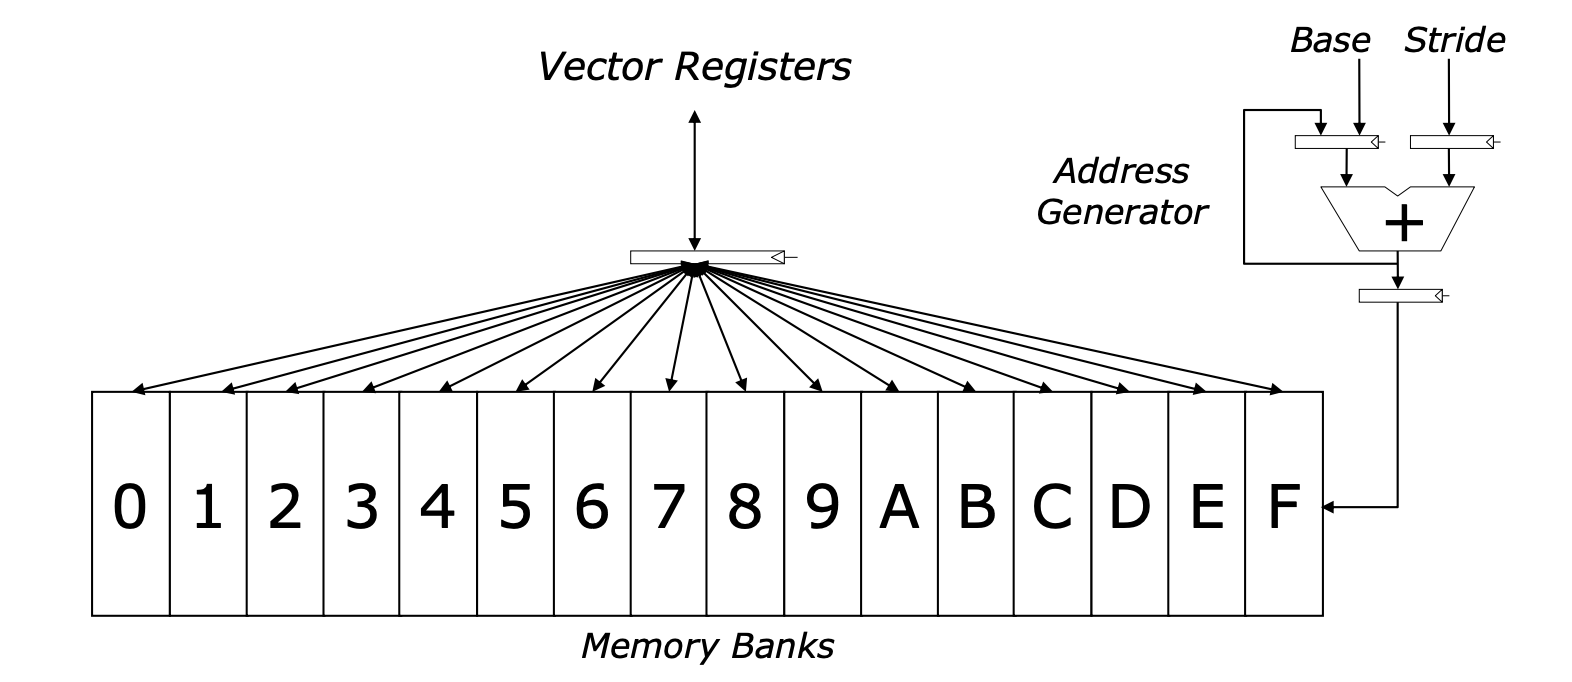
\includegraphics[width=1\linewidth]{assets/vector-mem-model.png}
    \caption{Vector memory system}
    \label{fig:enter-label}
\end{figure}

Trong sơ đồ thiết kế hệ thống, các thành phần chính bao gồm Memory Banks, Address Generator, Vector Registers và mối kết nối giữa chúng. Mỗi thành phần được giải thích chi tiết để làm rõ vai trò và ý nghĩa trong hoạt động của hệ thống.

Memory Banks nằm ở dưới cùng của sơ đồ, được đánh số từ 0 đến F (tổng cộng 16 bank trong hệ hexadecimal). Chúng chia nhỏ bộ nhớ để hỗ trợ truy cập song song, tăng băng thông tổng thể so với bộ nhớ đơn xử lý tuần tự. Trên Cray-1, mỗi bank có thời gian bận 4 chu kỳ sau khi được truy cập và độ trễ 12 chu kỳ để lấy dữ liệu. Tuy nhiên, nếu nhiều yêu cầu cùng nhắm đến một bank, xung đột bank (bank conflict) xảy ra, làm giảm hiệu suất.

Address Generator được đặt ở phía bên phải sơ đồ, nhận đầu vào từ Base (địa chỉ cơ sở) và Stride (khoảng cách giữa các phần tử). Bộ tạo địa chỉ sử dụng công thức Địa chỉ = Base + (Index × Stride) để sinh ra các địa chỉ bộ nhớ, cho phép truy cập linh hoạt cả dữ liệu liên tiếp và không liên tiếp, chẳng hạn trong xử lý ma trận. Dù vậy, stride không tối ưu có thể gây xung đột bank, ảnh hưởng tiêu cực đến hiệu suất.

Vector Registers nằm ở trên cùng, đóng vai trò lưu trữ tạm thời các vector từ Memory Banks. Nhờ vị trí gần bộ xử lý vector hơn so với bộ nhớ chính, chúng cung cấp dữ liệu nhanh chóng, giảm độ trễ và tăng hiệu suất xử lý. Dữ liệu được tải từ Memory Banks vào Vector Registers qua các kết nối song song, hỗ trợ hoạt động hiệu quả của hệ thống.

Cuối cùng, mối kết nối giữa Vector Registers và Memory Banks, biểu thị bằng các đường mũi tên, cho phép mỗi thanh ghi vector truy cập dữ liệu từ bất kỳ bank nào. Thiết kế này tối ưu hóa truy cập song song, cải thiện băng thông. Tuy nhiên, hiệu suất vẫn phụ thuộc vào việc tránh xung đột bank, vốn gây độ trễ 4 chu kỳ như đã đề cập, đòi hỏi sự tối ưu trong lập kế hoạch truy cập dữ liệu.

\subsubsection{Vector Chaining}
Dưới đây là phiên bản mở rộng của đoạn văn báo cáo khoa học, được viết dài hơn để cung cấp thêm chi tiết và giải thích rõ ràng hơn, vẫn giữ phong cách khoa học:

Kỹ thuật Vector Chaining là một phương pháp quan trọng trong kiến trúc các bộ xử lý vector, được thiết kế nhằm tối ưu hóa hiệu suất tính toán bằng cách liên kết các phép toán vector liên tiếp với nhau thông qua một cơ chế gọi là bypassing. Khác với cách xử lý truyền thống, trong đó một phép toán phải hoàn tất toàn bộ và ghi kết quả vào thanh ghi trước khi phép toán tiếp theo có thể bắt đầu, Vector Chaining cho phép phép toán tiếp theo được khởi động ngay khi dữ liệu từ phép toán trước đó sẵn sàng, loại bỏ thời gian chờ không cần thiết. Kỹ thuật này được xem như một phiên bản mở rộng của bypassing trong các bộ xử lý scalar, nơi kết quả của một phép toán được chuyển trực tiếp tới phép toán tiếp theo mà không cần qua bước trung gian ghi vào thanh ghi, nhờ đó giảm đáng kể độ trễ và tăng hiệu quả xử lý. Mục tiêu chính của Vector Chaining là nâng cao băng thông tính toán bằng cách tận dụng tối đa khả năng song song của các đơn vị chức năng trong bộ xử lý vector.
\begin{figure}[H]
    \centering
    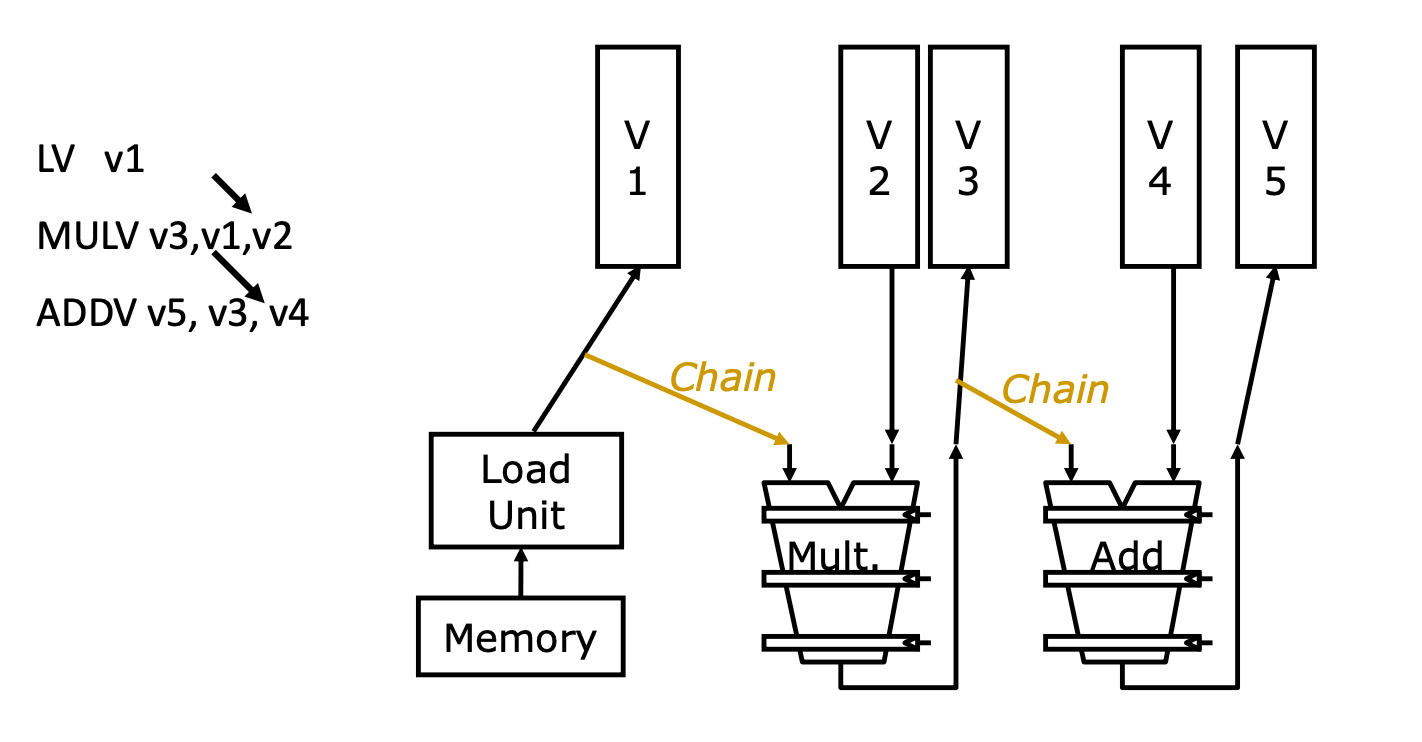
\includegraphics[width=1\linewidth]{assets/vector-chain.png}
    \caption{Enter Caption}
    \label{fig:enter-label}
\end{figure}
Sơ đồ minh họa quá trình Vector Chaining bao gồm các thành phần chính thể hiện cách dữ liệu di chuyển và được xử lý. Vector Registers, được đánh số từ V1 đến V5, là các thanh ghi lưu trữ tạm thời các vector, tức các mảng dữ liệu có thể chứa nhiều phần tử, chẳng hạn V1 lưu trữ 16 phần tử từ V1[0] đến V1[15]. Load Unit chịu trách nhiệm tải dữ liệu từ Memory – nơi lưu trữ chính của hệ thống – vào thanh ghi vector V1 để chuẩn bị cho các phép toán tiếp theo. Hai Functional Units bao gồm Mult. Unit, thực hiện phép nhân vector, và Add Unit, thực hiện phép cộng vector, đóng vai trò xử lý các phép toán số học trên dữ liệu vector. Đặc biệt, các đường màu vàng được đánh dấu "Chain" trong sơ đồ thể hiện cơ chế Vector Chaining, cho thấy dữ liệu được chuyển trực tiếp từ một đơn vị chức năng này sang đơn vị chức năng khác mà không cần quay lại thanh ghi trung gian, tạo nên một luồng xử lý liền mạch.

Chuỗi các lệnh vector trong sơ đồ bao gồm ba bước cụ thể. Đầu tiên, lệnh LV V1 (Load Vector) tải dữ liệu từ bộ nhớ vào thanh ghi V1, ví dụ như 16 phần tử liên tiếp từ một địa chỉ bộ nhớ xác định. Tiếp theo, lệnh MULV V3, V1, V2 (Multiply Vector) thực hiện phép nhân từng phần tử giữa V1 và V2, với kết quả được lưu vào V3 theo công thức V3[i] = V1[i] × V2[i], trong đó i chạy từ 0 đến độ dài vector trừ 1 (ví dụ, 15 nếu vector có 16 phần tử). Cuối cùng, lệnh ADDV V5, V3, V4 (Add Vector) cộng từng phần tử của V3 với V4, lưu kết quả vào V5 theo công thức V5[i] = V3[i] + V4[i], với cùng phạm vi chỉ số i. Các phép toán này được thực hiện trên toàn bộ vector, nhưng nhờ Vector Chaining, chúng không cần đợi toàn bộ vector được xử lý xong ở mỗi bước.

Cơ chế Vector Chaining trong sơ đồ được thể hiện qua hai "chuỗi" chính. Chain 1 xảy ra giữa Load Unit và Mult. Unit: ngay khi một phần tử của V1, chẳng hạn V1[0], được tải từ bộ nhớ, nó được chuyển trực tiếp đến Mult. Unit để nhân với V2[0], tạo ra V3[0], mà không cần chờ toàn bộ vector V1 được tải xong. Tương tự, Chain 2 giữa Mult. Unit và Add Unit cho phép phần tử V3[0], ngay sau khi được tính toán, được gửi thẳng tới Add Unit để cộng với V4[0], tạo ra V5[0], thay vì đợi toàn bộ V3 hoàn tất và ghi vào thanh ghi. Cách tiếp cận này tận dụng tính chất pipeline của bộ xử lý vector, cho phép xử lý song song từng phần tử (element-wise parallelism), làm tăng hiệu suất đáng kể so với phương pháp tuần tự.

Để hiểu rõ hơn hiệu quả của Vector Chaining, có thể so sánh hai kịch bản. Nếu không sử dụng chaining, với một vector 16 phần tử, quy trình sẽ diễn ra tuần tự: Load V1 mất 16 chu kỳ để tải toàn bộ vector, MULV V3, V1, V2 mất thêm 16 chu kỳ để hoàn tất phép nhân, và ADDV V5, V3, V4 mất tiếp 16 chu kỳ cho phép cộng, dẫn đến tổng cộng 48 chu kỳ. Ngược lại, với Vector Chaining, các phép toán được pipeline hóa: sau khi phần tử đầu tiên (V1[0]) được tải (1 chu kỳ), nhân (1 chu kỳ), và cộng (1 chu kỳ) – tổng cộng 3 chu kỳ khởi đầu – mỗi phần tử tiếp theo chỉ mất thêm 1 chu kỳ nhờ các đơn vị chức năng hoạt động đồng thời. Do đó, tổng thời gian cho 16 phần tử là 3 + (16 - 1) × 1 = 18 chu kỳ. Kết quả cho thấy Vector Chaining giảm thời gian thực thi từ 48 chu kỳ xuống 18 chu kỳ trong ví dụ này, minh chứng cho khả năng cải thiện hiệu suất vượt trội bằng cách giảm thời gian chờ và tối ưu hóa luồng xử lý các phép toán vector liên tiếp.

Trong bối cảnh minh họa, các vector v1, v2, v3, v4, v5 đều có độ dài 4 phần tử, được định nghĩa như sau: v1 = [a0, a1, a2, a3], v2 = [b0, b1, b2, b3], và v4 = [d0, d1, d2, d3]. Quá trình xử lý dữ liệu sử dụng ba lệnh vector cơ bản bao gồm: Load để tải dữ liệu từ bộ nhớ vào thanh ghi vector, Mul để thực hiện phép nhân vector, và Add để thực hiện phép cộng vector. Các lệnh này được phân tích trong hai kịch bản: không áp dụng Vector Chaining và có áp dụng Vector Chaining, nhằm đánh giá sự khác biệt về hiệu suất.
\begin{figure}[H]
    \centering
    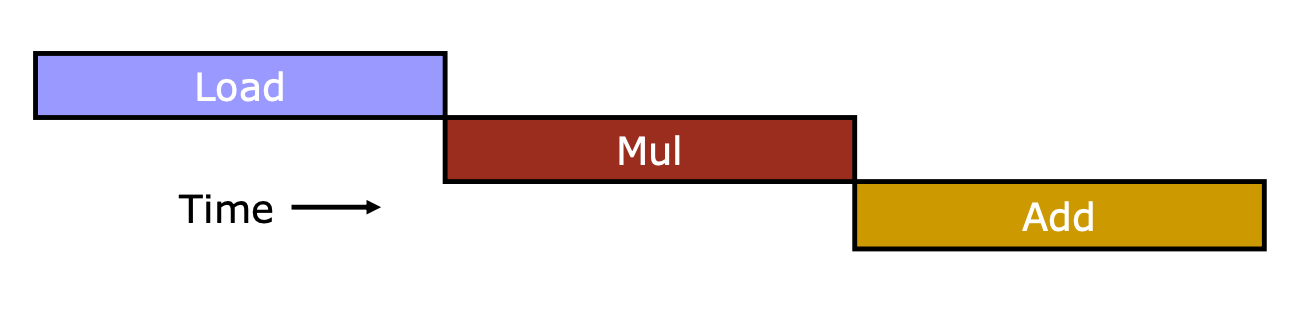
\includegraphics[width=0.6\linewidth]{assets/vector-chain-1.png}
    \caption{Enter Caption}
    \label{fig:enter-label}
\end{figure}
Khi không sử dụng Vector Chaining, các lệnh được thực hiện theo cách tuần tự, yêu cầu mỗi lệnh phải hoàn tất toàn bộ – bao gồm việc ghi kết quả vào thanh ghi – trước khi lệnh tiếp theo có thể bắt đầu. Cụ thể, lệnh LV v1 tải toàn bộ vector v1 từ bộ nhớ vào thanh ghi mất 4 chu kỳ, với mỗi phần tử được xử lý trong 1 chu kỳ. Sau khi v1 được tải xong, lệnh MULV v3, v1, v2 bắt đầu, thực hiện phép nhân từng cặp phần tử v1[i] × v2[i] để tạo ra v3[i] (i = 0, 1, 2, 3), cũng mất 4 chu kỳ. Tiếp theo, lệnh ADDV v5, v3, v4 thực hiện phép cộng từng cặp v3[i] + v4[i] để tạo v5[i], mất thêm 4 chu kỳ. Tổng thời gian trong trường hợp này là 4 + 4 + 4 = 12 chu kỳ, chưa tính đến các độ trễ pipeline bổ sung.
\begin{figure}[H]
    \centering
    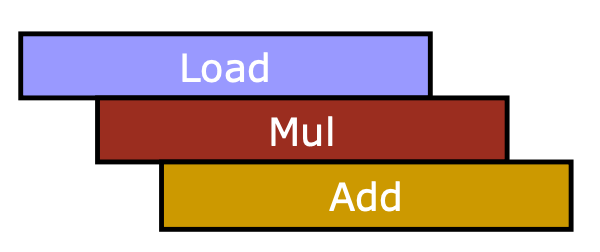
\includegraphics[width=0.5\linewidth]{assets/vector-chain-2.png}
    \caption{Enter Caption}
    \label{fig:enter-label}
\end{figure}
Ngược lại, khi áp dụng Vector Chaining, các lệnh có thể bắt đầu ngay khi phần tử đầu tiên từ lệnh trước sẵn sàng, nhờ cơ chế chuyển dữ liệu trực tiếp giữa các đơn vị chức năng mà không cần chờ ghi vào thanh ghi. Quá trình bắt đầu với chu kỳ 1, khi v1[0] được tải từ bộ nhớ và ngay lập tức chuyển đến đơn vị nhân để tính v3[0] = v1[0] × v2[0]. Đến chu kỳ 2, v1[1] được tải, v3[1] = v1[1] × v2[1] được tính, đồng thời v3[0] được chuyển đến đơn vị cộng để tính v5[0] = v3[0] + v4[0]. Quy trình này tiếp diễn, với Load kết thúc ở chu kỳ 4, Mul bắt đầu từ chu kỳ 2 và kết thúc ở chu kỳ 5, và Add bắt đầu từ chu kỳ 3 và kết thúc ở chu kỳ 6. Nhờ sự song song hóa, tổng thời gian giảm xuống còn 6 chu kỳ.

So sánh hiệu suất giữa hai kịch bản cho thấy sự khác biệt rõ rệt. Trong trường hợp không có Vector Chaining, tổng thời gian là 12 chu kỳ do các lệnh phải chờ nhau tuần tự, dẫn đến thời gian thực thi kéo dài. Ngược lại, với Vector Chaining, tổng thời gian chỉ còn 6 chu kỳ nhờ tận dụng pipeline và giảm thiểu độ trễ khởi động giữa các đơn vị chức năng. Điều này thể hiện hiệu quả vượt trội của kỹ thuật chaining trong việc tối ưu hóa luồng xử lý.

Lợi ích của Vector Chaining được minh họa rõ ràng qua ví dụ này. Kỹ thuật này giảm gần một nửa thời gian thực thi (từ 12 chu kỳ xuống 6 chu kỳ), đồng thời tăng hiệu suất bằng cách duy trì hoạt động liên tục của các đơn vị chức năng như Load, Multiply, và Add. Nhờ đó, thời gian nhàn rỗi giữa các bước xử lý được loại bỏ, giúp hệ thống hoạt động hiệu quả hơn trong các ứng dụng yêu cầu xử lý vector nhanh chóng và liên tục.
\subsubsection{Vector Instruction-Level Parallelism}
Vector Instruction-Level Parallelism (ILP) là một kỹ thuật trong kiến trúc máy vector, cho phép thực thi đồng thời nhiều lệnh vector trên các đơn vị chức năng riêng biệt, bổ sung thêm một tầng song song hóa so với tính song song ở cấp độ dữ liệu (data-level parallelism) vốn đã được hỗ trợ bởi các lanes trong một đơn vị chức năng. Trong khi song song hóa dữ liệu (SIMD - Single Instruction, Multiple Data) thực hiện một phép toán duy nhất trên nhiều phần tử cùng lúc (ví dụ: lệnh ADDV cộng đồng thời 32 phần tử), Vector ILP nâng cao hiệu suất bằng cách cho phép nhiều lệnh vector khác nhau – như lệnh tải (load), nhân (multiply), và cộng (add) – được thực thi song song trên các đơn vị chức năng tương ứng, qua đó tăng thông lượng tổng thể. Hình minh họa thể hiện một máy vector với thanh ghi chứa 32 phần tử, 8 lanes mỗi đơn vị chức năng (Load Unit, Multiply Unit, Add Unit), đạt hiệu suất 24 phép toán mỗi chu kỳ trong khi chỉ phát ra dưới 1 lệnh ngắn mỗi chu kỳ.
\begin{figure}[H]
    \centering
    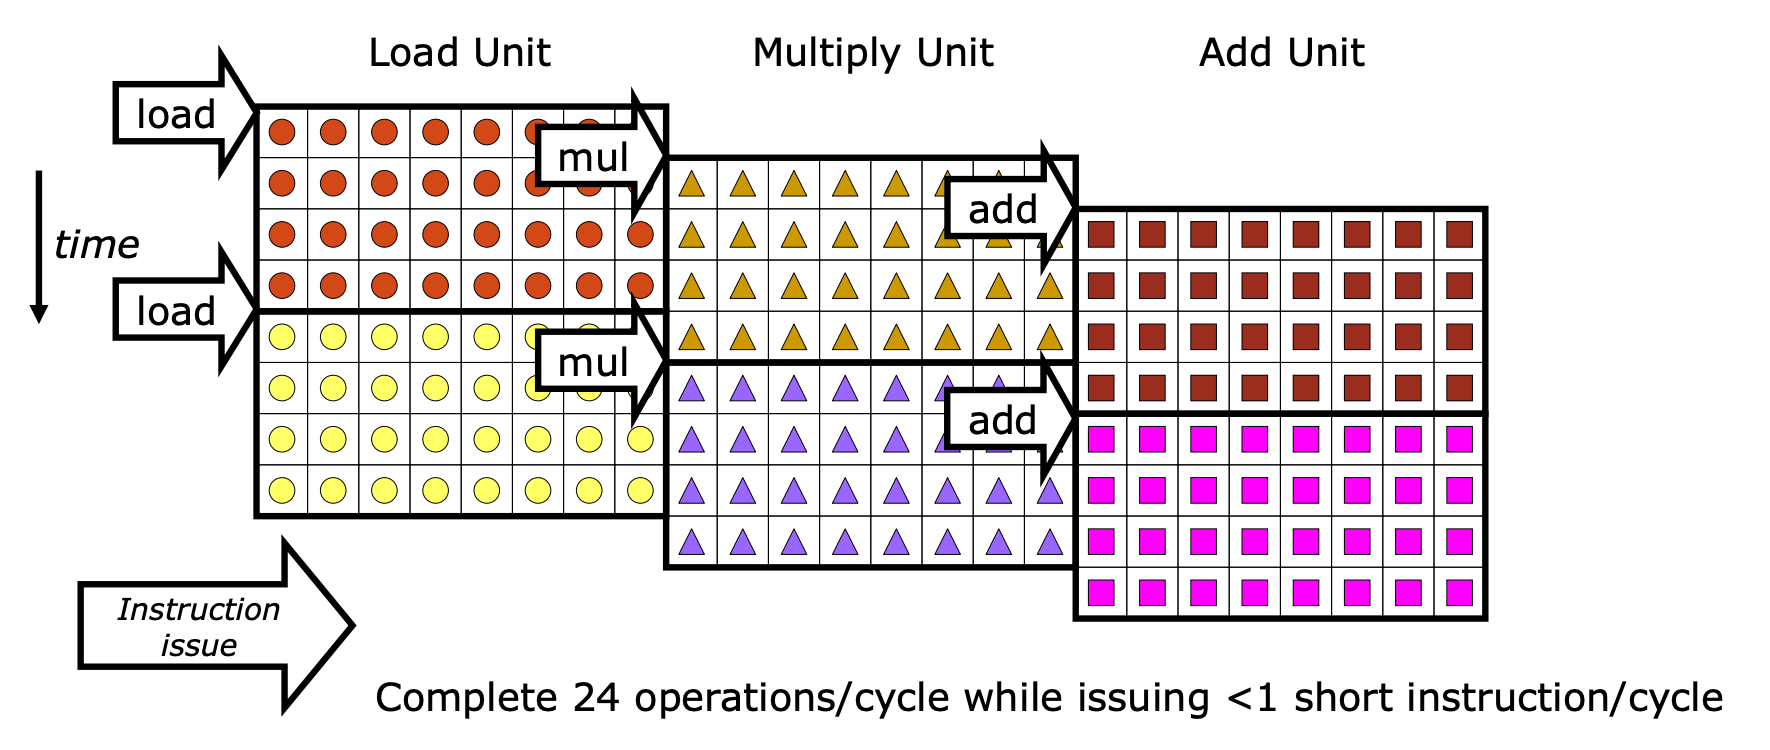
\includegraphics[width=1\linewidth]{assets/vector-instruction-level.png}
    \caption{Enter Caption}
    \label{fig:enter-label}
\end{figure}
Cụ thể, mỗi thanh ghi vector lưu trữ 32 phần tử (tương đương 128 byte với số thực 32-bit), và 8 lanes cho phép mỗi đơn vị chức năng xử lý 8 phần tử mỗi chu kỳ, dẫn đến một lệnh vector (như LV, MULV, ADDV) mất 4 chu kỳ để hoàn thành. Load Unit tải dữ liệu từ bộ nhớ vào thanh ghi vector, với hai lệnh load (màu đỏ và vàng) thực thi song song nếu băng thông bộ nhớ đủ lớn, mỗi chu kỳ xử lý 8 phần tử. Multiply Unit thực hiện phép nhân vector, với hai lệnh nhân (màu vàng và tím) hoạt động đồng thời trên các cặp phần tử độc lập, cũng xử lý 8 phép nhân mỗi chu kỳ. Tương tự, Add Unit xử lý hai lệnh cộng (màu nâu và hồng) song song, thực hiện 8 phép cộng mỗi chu kỳ. Trục thời gian dọc (tăng từ trên xuống) và trục phát lệnh ngang (từ trái sang phải) trong hình cho thấy các lệnh được phân bổ và thực thi hiệu quả qua từng chu kỳ.

Hiệu suất đạt được là 24 phép toán mỗi chu kỳ, bao gồm 8 phép load, 8 phép nhân, và 8 phép cộng từ ba đơn vị chức năng, trong khi tốc độ phát lệnh trung bình dưới 1 lệnh mỗi chu kỳ (ví dụ: 0.25 lệnh/chu kỳ nếu phát 1 lệnh mỗi 4 chu kỳ). Để minh họa, xét chuỗi lệnh: LV v1 và LV v2 tải dữ liệu, MULV v3, v1, v2 và MULV v4, v5, v6 thực hiện phép nhân, ADDV v7, v3, v4 và ADDV v8, v9, v10 thực hiện phép cộng. Trong chu kỳ 1, Load Unit bắt đầu tải v1, Multiply Unit thực hiện MULV v4, v5, v6, và Add Unit thực hiện ADDV v8, v9, v10 (giả sử v5, v6, v9, v10 đã sẵn sàng). Đến chu kỳ 2, Load Unit tiếp tục v1 và bắt đầu v2, các đơn vị còn lại tiếp tục công việc. Đến chu kỳ 5, sau khi v1, v2 hoàn tất, Multiply Unit bắt đầu MULV v3, v1, v2, và đến chu kỳ 9, Add Unit thực hiện ADDV v7, v3, v4. Nhờ Vector ILP, các đơn vị chức năng luôn hoạt động tối đa, đạt hiệu suất cao với thông lượng lớn mà không cần tăng đáng kể số lệnh phát ra, minh chứng cho hiệu quả của song song hóa ở cấp độ lệnh trong máy vector.

\subsection{Mạng nơ-ron}
\subsubsection{Sự phát triển của mạng nơ-ron}
Quá trình phát triển của mạng nơ-ron có thể được chia đại khái thành năm giai đoạn: giai đoạn đề xuất mô hình, thời kỳ đình trệ, sự nổi lên của thuật toán lan truyền ngược, thời kỳ bối rối, và sự phát triển của học sâu.
Giai đoạn từ năm 1943 đến 1958 được coi là giai đoạn đề xuất mô hình, và làn sóng perceptron được đề xuất vào năm 1958 kéo dài khoảng 10 năm. Khi ngày càng nhiều học giả tham gia vào hướng nghiên cứu này, một số học giả dần phát hiện ra những hạn chế của mô hình perceptron. Với việc xuất bản cuốn \textbf{Perceptron} của M. Minsky vào năm 1969, mạng nơ-ron bị đẩy xuống đáy, dẫn đến "thời kỳ đình trệ" của mạng nơ-ron từ năm 1969 đến 1980.
\begin{figure}[H]
    \centering
    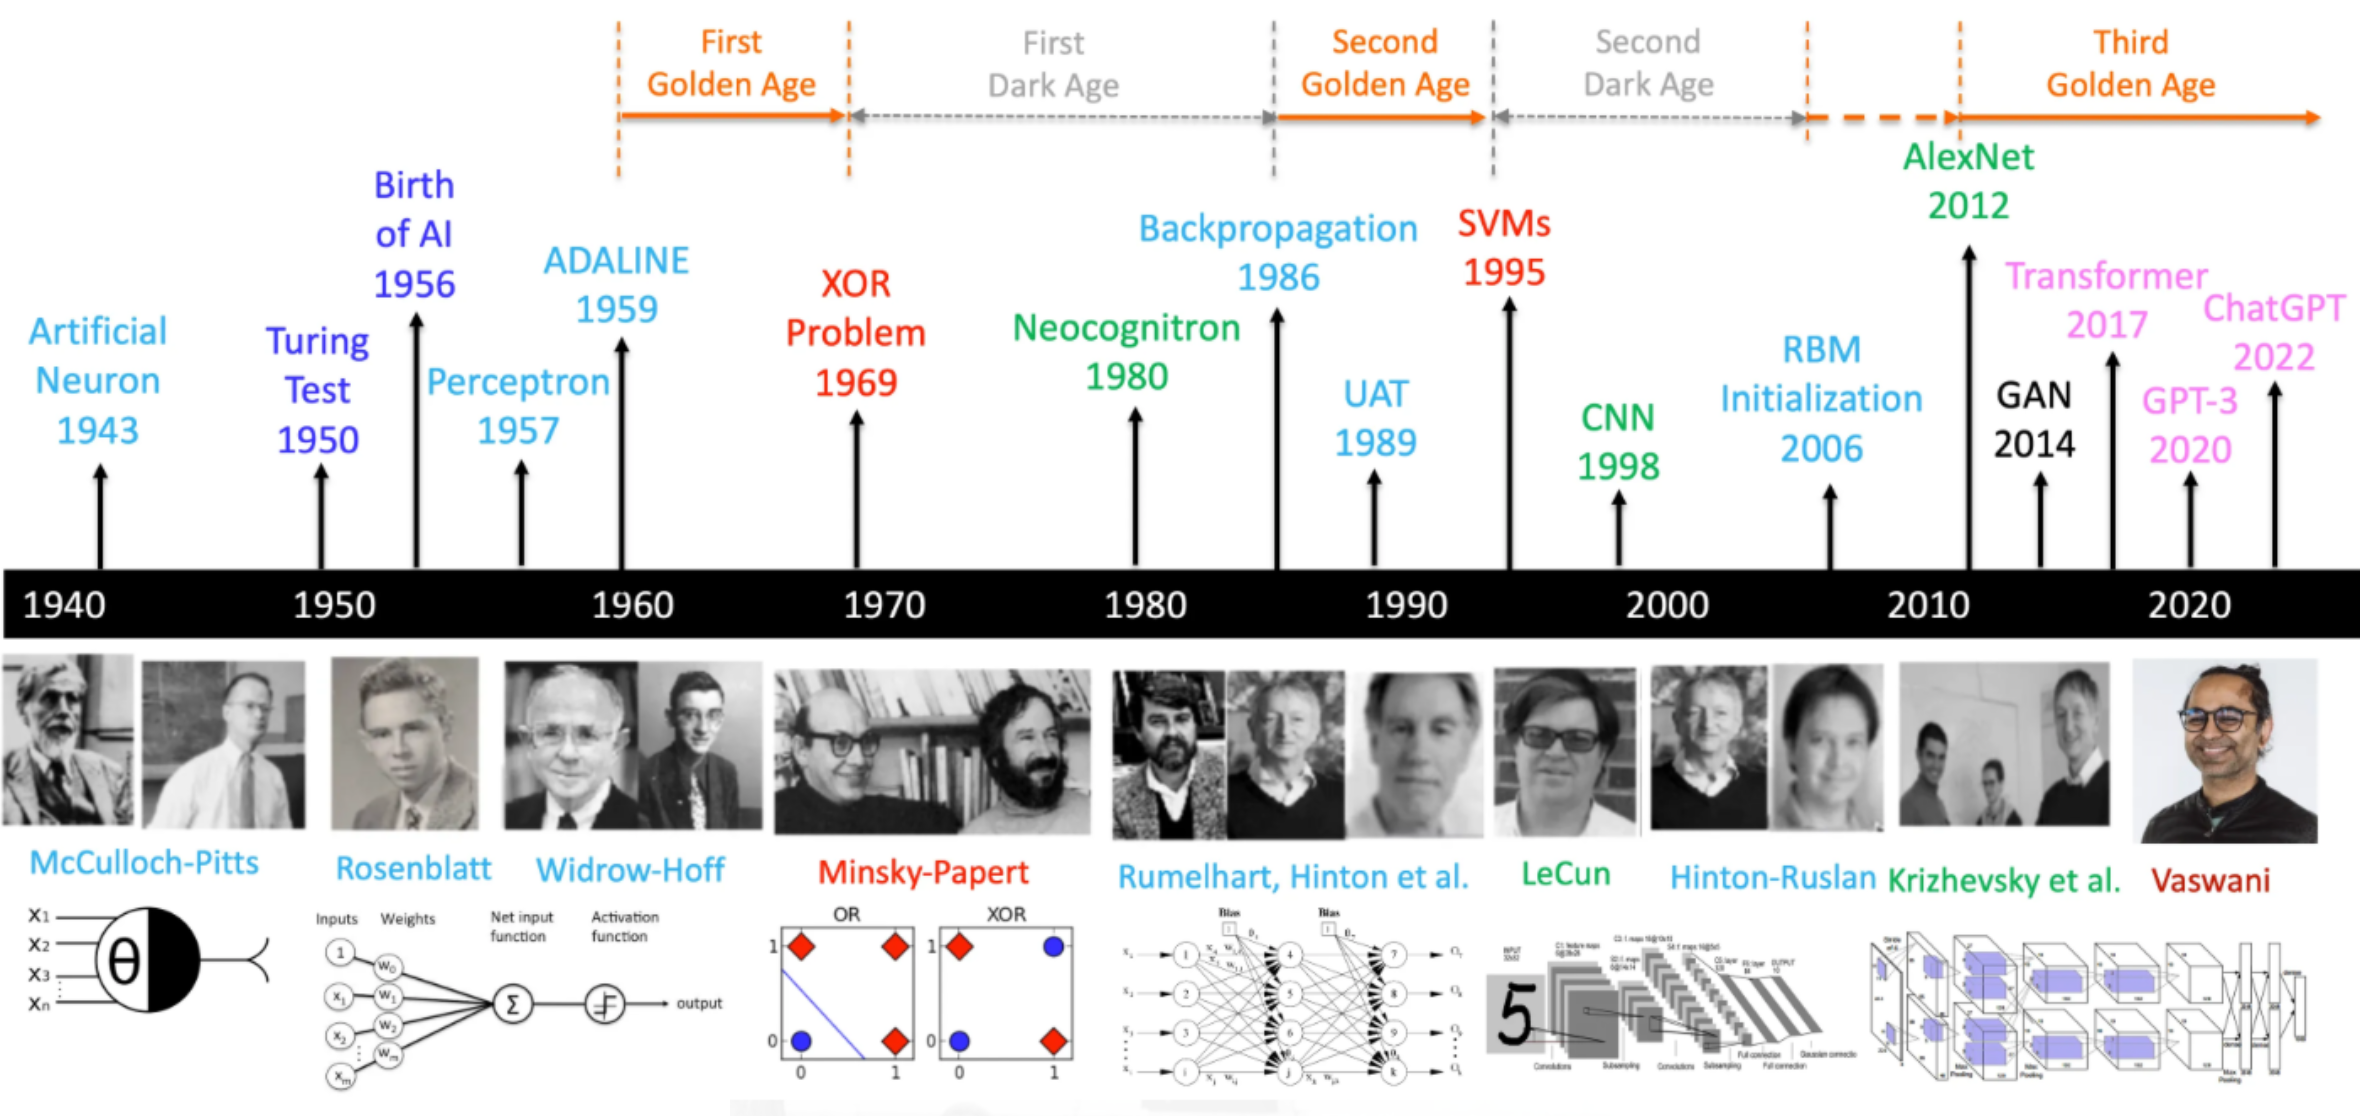
\includegraphics[width=1\linewidth]{assets/dl-history.png}
    \caption{Lịch sử deep learning}
    \label{fig:enter-label}
\end{figure}
Sau năm 1980, ngày càng nhiều học giả chú ý đến thuật toán lan truyền ngược, điều này đã mở lại tư duy cho các nhà nghiên cứu và khởi đầu một mùa xuân khác cho sự phát triển của mạng nơ-ron.

Sau đó, trong một thời gian dài, các học giả không đạt được kết quả đột phá, chỉ làm việc dựa trên các nghiên cứu hiện có. Vào giữa những năm 1990, lý thuyết học thống kê và mô hình học máy được đại diện bởi máy vector hỗ trợ bắt đầu nổi lên. Ngược lại, cơ sở lý thuyết của mạng nơ-ron không rõ ràng, và các khó khăn về tối ưu hóa, khả năng giải thích kém cùng các nhược điểm khác trở nên nổi bật hơn; do đó, nghiên cứu mạng nơ-ron lại rơi vào giai đoạn thoái trào.

Cho đến năm 2006, Giáo sư Geoffrey Hinton, một chuyên gia về mạng nơ-ron tại Đại học Toronto, cùng các học trò của mình chính thức đề xuất khái niệm học sâu. Họ đã đề xuất mô hình mạng niềm tin sâu trong bài báo được công bố. Hinton và các cộng sự [26] phát hiện rằng mạng nơ-ron tiến tới đa tầng có thể được huấn luyện trước từng tầng. Nói cách khác, phương pháp huấn luyện trước không giám sát được sử dụng để cải thiện giá trị ban đầu của trọng số mạng, sau đó các trọng số được tinh chỉnh. Mô hình này đã khởi đầu làn sóng nghiên cứu về mạng nơ-ron sâu và mở đầu cho việc nghiên cứu và ứng dụng học sâu.

Hiện nay, các mô hình học sâu phổ biến bao gồm mạng nơ-ron sâu (DNN), mạng nơ-ron tích chập (CNN), mạng nơ-ron hồi quy (RNN) và mạng đối kháng sinh tạo (GAN), cùng nhiều mô hình khác.
\subsubsection{DNN}

Vì perceptron đơn tầng không thể giải quyết vấn đề không phân tách tuyến tính, nó không thể được sử dụng trong công nghiệp. Các học giả đã mở rộng và cải tiến mô hình perceptron bằng cách tăng số lượng tầng ẩn và các nút tương ứng để nâng cao khả năng biểu đạt của mô hình, từ đó mạng nơ-ron sâu (DNN) ra đời. DNN đôi khi được gọi là perceptron đa tầng (MLP). Sự xuất hiện của DNN đã khắc phục hiệu suất thấp của perceptron đơn tầng. Theo vị trí của các tầng khác nhau trong DNN, các tầng mạng nơ-ron bên trong DNN có thể được chia thành ba loại: tầng đầu vào, tầng ẩn và tầng đầu ra, như được thể hiện trong Hình 2. Nói chung, tầng đầu tiên là tầng đầu vào, tầng cuối cùng là tầng đầu ra, và các tầng ở giữa đều là tầng ẩn. Các tầng được kết nối đầy đủ với nhau, nghĩa là bất kỳ nơ-ron nào ở tầng n phải được kết nối với bất kỳ nơ-ron nào ở tầng n+1. Mặc dù DNN có vẻ phức tạp, nhưng từ một mô hình cục bộ nhỏ, nó giống như perceptron, tức là một quan hệ tuyến tính \( z = \sum W_i X_i + b \) cộng với một hàm kích hoạt \( \sigma(z) \).

\begin{figure}
    \centering
    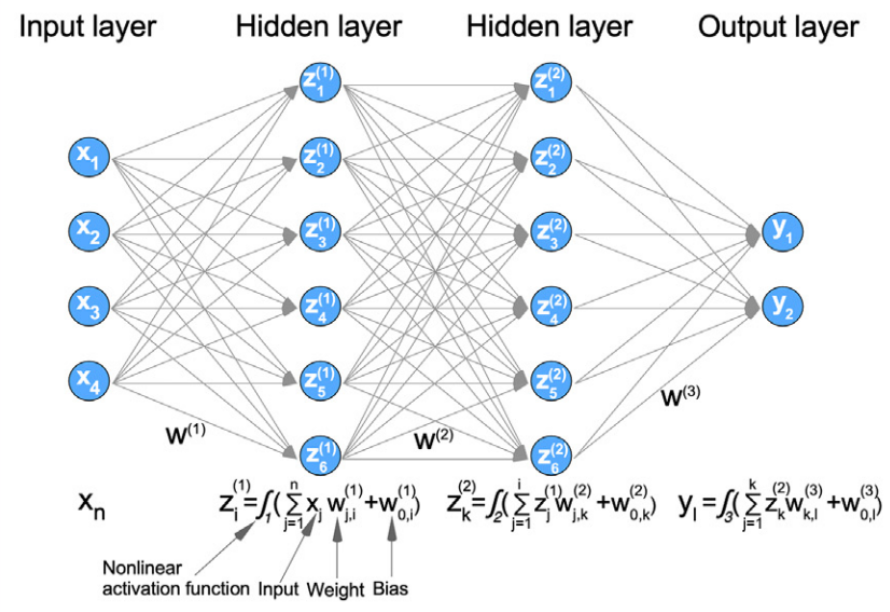
\includegraphics[width=0.75\linewidth]{assets/dnn.png}
    \caption{DNN network}
    \label{fig:enter-label}
\end{figure}

Với việc các tầng của mạng nơ-ron ngày càng sâu hơn, các hiện tượng như quá khớp (overfitting), nổ gradient và biến mất gradient trở nên nghiêm trọng hơn, và hàm tối ưu ngày càng dễ rơi vào giải pháp tối ưu cục bộ. Để khắc phục vấn đề này, các học giả đã đề xuất mạng nơ-ron tích chập (CNN) dựa trên cơ chế trường tiếp nhận trong sinh học.

\subsubsection{CNN}
Mô hình CNN được phát triển từ mạng nơ-ron nhân tạo ban đầu. Dựa trên nghiên cứu của Hub và các cộng sự về tế bào trong vỏ não thị giác của mèo, mô hình CNN là một mạng nơ-ron nhân tạo được thiết kế đặc biệt với nhiều tầng ẩn thông qua lớp vỏ não mô phỏng sinh học. Phép toán tích chập được sử dụng để giải quyết nhược điểm của việc tính toán lớn và mất thông tin cấu trúc của mạng nơ-ron nhân tạo. Năm 1982, Fukushima và các cộng sự đã đề xuất khái niệm Neocognitron để mô phỏng chức năng nhận thức thị giác của con người, được coi là điểm khởi đầu của CNN. Năm 1989, LeCun và các cộng sự xây dựng mô hình Le-Net ban đầu, bao gồm một tầng tích chập và một tầng kết nối đầy đủ. Năm 1998, LeCun và các cộng sự đã cải tiến và đề xuất mô hình LeNet-5 cổ điển, giải quyết tốt hơn vấn đề nhận diện chữ số viết tay.

Sự ra đời của LeNet-5 đã thiết lập dạng phôi thai cơ bản của CNN, bao gồm tầng tích chập, tầng gộp (pooling), hàm kích hoạt và tầng kết nối đầy đủ được kết nối theo một số lượng trình tự nhất định, như được thể hiện trong hình. CNN chủ yếu được áp dụng cho phân loại hình ảnh, phát hiện đối tượng, và phân đoạn ngữ nghĩa, cũng như trong các lĩnh vực khác. Các thuật toán phổ biến nhất là YOLO và R-CNN, trong đó YOLO có tốc độ nhận diện nhanh hơn nhờ đặc điểm của thuật toán và đã được nâng cấp lên phiên bản V7. Thuật toán tìm kiếm và nhận diện vị trí mục tiêu của R-CNN hơi khác so với YOLO. Mặc dù tốc độ chậm hơn YOLO, nhưng độ chính xác của R-CNN lại cao hơn.

\begin{figure}
    \centering
    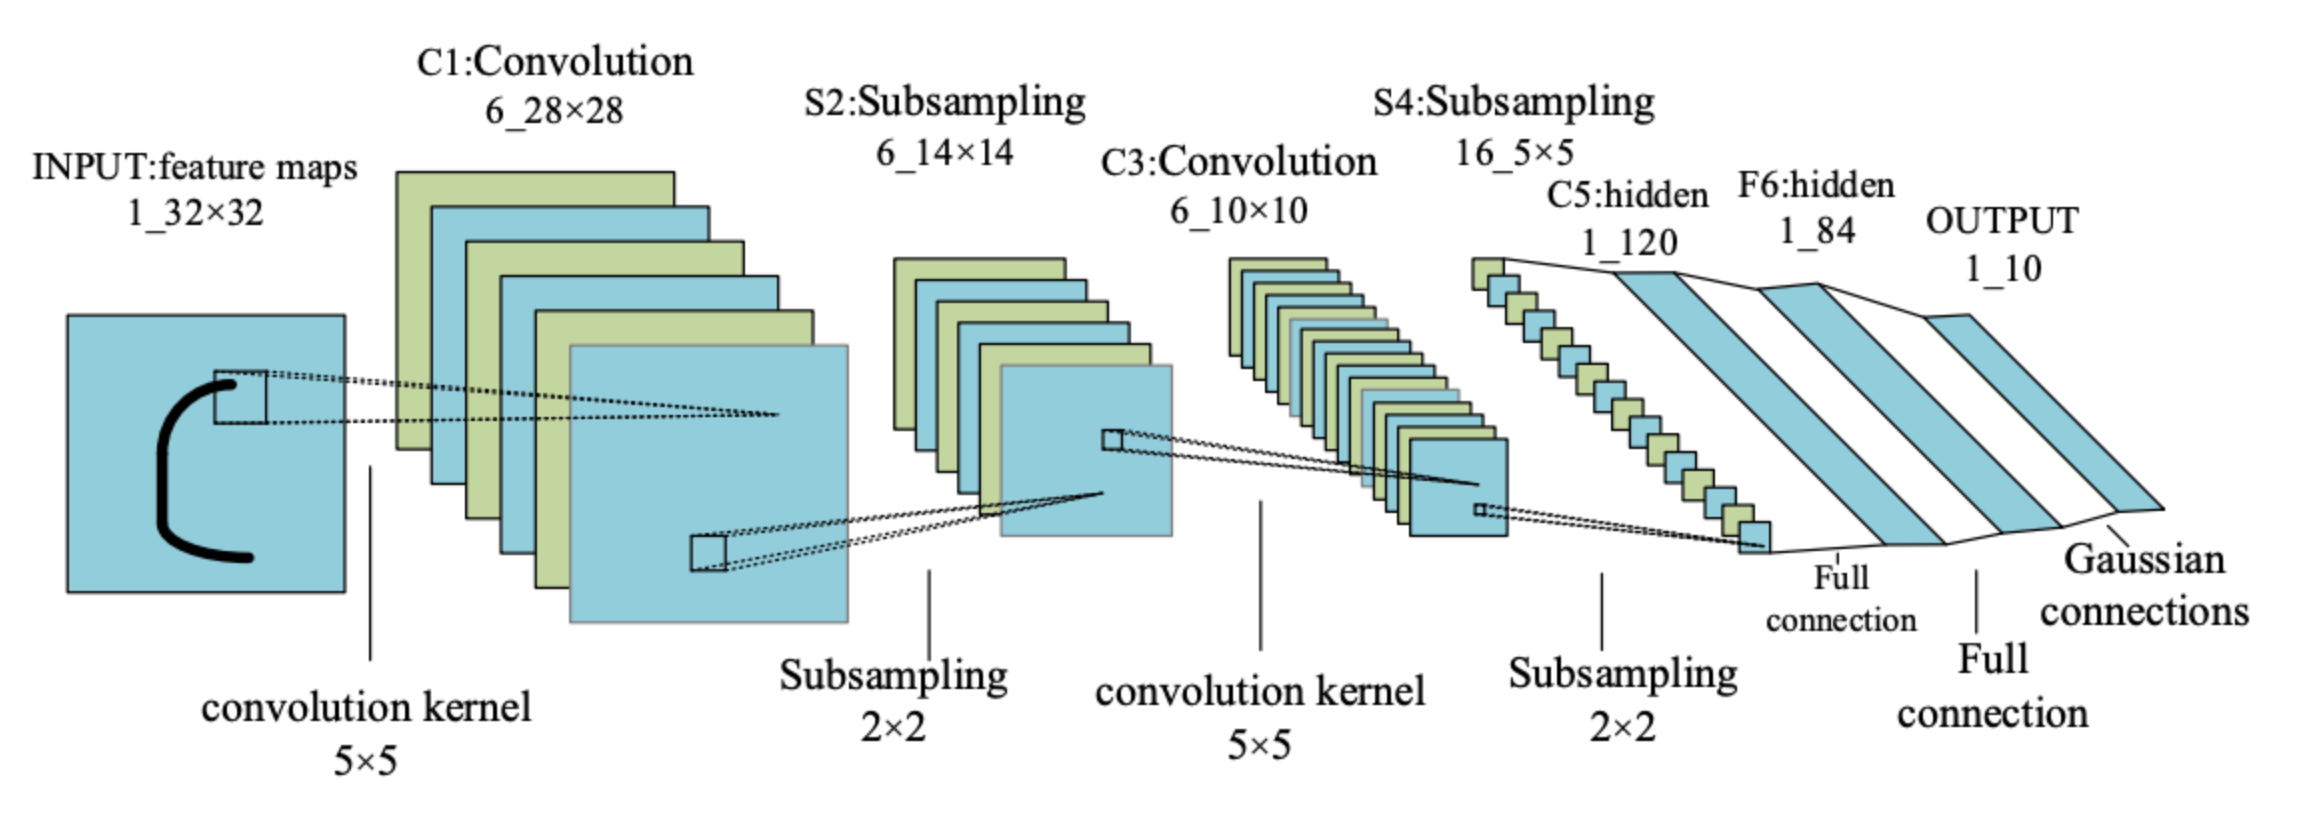
\includegraphics[width=1\linewidth]{assets/cnn-network.png}
    \caption{CNN network}
    \label{fig:enter-label}
\end{figure}

Mạng nơ-ron tích chập có hai đặc điểm là nhận thức cục bộ và chia sẻ tham số. Nhận thức cục bộ nghĩa là mạng nơ-ron tích chập đề xuất rằng mỗi nơ-ron không cần cảm nhận tất cả các pixel trong hình ảnh mà chỉ cảm nhận các pixel cục bộ trong hình ảnh; sau đó, ở mức độ cao hơn, thông tin của các pixel cục bộ này được hợp nhất để thu được toàn bộ thông tin của hình ảnh. Các đơn vị nơ-ron của các tầng khác nhau được kết nối cục bộ, nghĩa là các đơn vị nơ-ron của mỗi tầng chỉ kết nối với một phần các đơn vị nơ-ron của tầng trước đó. Mỗi đơn vị nơ-ron chỉ phản hồi với khu vực trong trường tiếp nhận và hoàn toàn không xem xét khu vực ngoài trường tiếp nhận. Mẫu kết nối cục bộ này đảm bảo rằng tích chập học được có phản hồi mạnh nhất với mẫu cục bộ không gian của đầu vào. Cấu trúc mạng chia sẻ trọng số làm cho nó giống với mạng nơ-ron sinh học hơn, giảm độ phức tạp của mô hình mạng và giảm số lượng trọng số. Cấu trúc mạng này có tính bất biến cao đối với dịch chuyển, tỷ lệ, nghiêng hoặc các dạng biến dạng khác. Ngoài ra, mạng nơ-ron tích chập sử dụng hình ảnh gốc làm đầu vào, có thể học hiệu quả các đặc trưng tương ứng từ một lượng lớn mẫu và tránh quá trình trích xuất đặc trưng phức tạp.

Do mạng nơ-ron tích chập có thể xử lý trực tiếp hình ảnh hai chiều, nó đã được ứng dụng rộng rãi trong xử lý hình ảnh và đạt được nhiều thành tựu nghiên cứu. Mạng trích xuất các đặc trưng trừu tượng hơn từ hình ảnh gốc thông qua các mô hình phi tuyến đơn giản và chỉ yêu cầu sự tham gia tối thiểu của con người trong toàn bộ quá trình. Tuy nhiên, vì tín hiệu của mỗi tầng chỉ có thể lan truyền theo một hướng và việc xử lý mẫu là độc lập với nhau tại mỗi thời điểm, cả DNN lẫn CNN đều không thể mô hình hóa các thay đổi trong chuỗi thời gian. Tuy nhiên, trong xử lý ngôn ngữ tự nhiên, nhận diện giọng nói, nhận diện chữ viết tay và các lĩnh vực khác, thứ tự thời gian của mẫu rất quan trọng, và cả DNN lẫn CNN đều không thể xử lý các kịch bản này. Do đó, mạng nơ-ron hồi quy (RNN) ra đời.
\subsubsection{RNN}
Khác với CNN, RNN đưa vào chiều "thời gian", phù hợp để xử lý dữ liệu kiểu chuỗi thời gian. Vì mạng này có khả năng ghi nhớ, nó có thể học các loại dữ liệu có mối tương quan trước và sau. Mạng nơ-ron hồi quy có khả năng khớp mô hình mạnh mẽ đối với dữ liệu chuỗi hóa và được ứng dụng rộng rãi trong lĩnh vực xử lý ngôn ngữ tự nhiên (NLP), bao gồm phân loại hình ảnh, thu thập hình ảnh, dịch máy, xử lý video, phân tích cảm xúc và tính toán độ tương đồng văn bản. Cấu trúc cụ thể như sau: mạng nơ-ron hồi quy sẽ lưu trữ và ghi nhớ thông tin trước đó trong tầng ẩn, sau đó đưa vào phép tính hiện tại của đơn vị tầng ẩn.

\begin{figure}
    \centering
    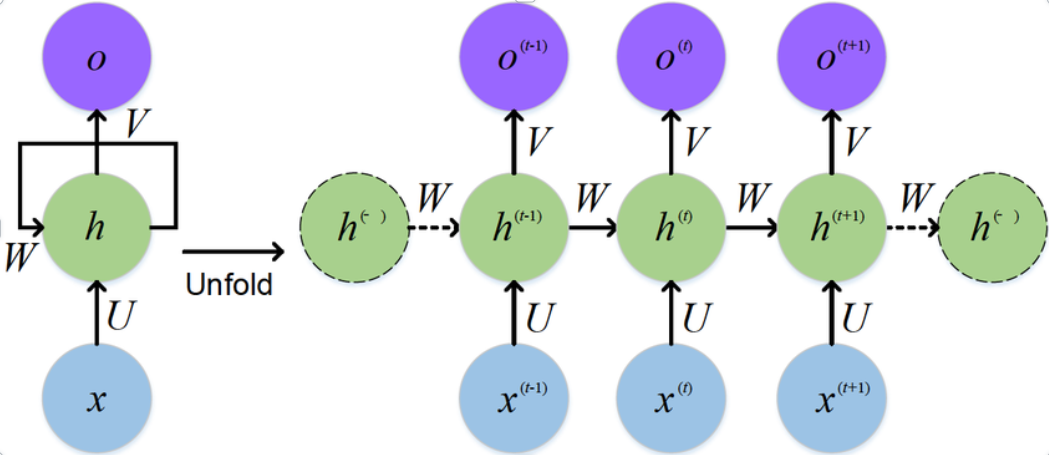
\includegraphics[width=1\linewidth]{assets/rnn.png}
    \caption{RNN network}
    \label{fig:enter-label}
\end{figure}
Hình trên cho thấy cấu trúc điển hình của RNN, tương tự nhưng khác với mạng nơ-ron sâu truyền thống (DNN). Điểm tương đồng là mô hình mạng của DNN và RNN đều được kết nối đầy đủ từ tầng đầu vào đến tầng ẩn rồi đến tầng đầu ra, và quá trình lan truyền mạng cũng theo thứ tự. Điểm khác biệt là các nút bên trong tầng ẩn của RNN không còn độc lập với nhau mà có thông điệp truyền qua lại. Đầu vào của tầng ẩn có thể bao gồm đầu ra của tầng đầu vào và đầu ra của tầng ẩn tại thời điểm trước đó, điều này cho thấy các nút trong tầng ẩn tự kết nối với nhau. Nó cũng có thể bao gồm đầu ra của tầng đầu vào, đầu ra của tầng ẩn tại thời điểm trước và trạng thái của tầng ẩn trước đó, điều này cho thấy các nút trong tầng ẩn không chỉ tự kết nối mà còn kết nối lẫn nhau.

Mặc dù RNN giải quyết được các vấn đề mà CNN không thể xử lý, nó vẫn có một số nhược điểm. Do đó, có nhiều biến thể của RNN, trong đó mạng dài ngắn hạn (LSTM) là một trong những mạng được sử dụng phổ biến nhất. Dữ liệu đầu vào của các mạng này không bị giới hạn ở hình ảnh hoặc văn bản, và vấn đề được giải quyết không chỉ giới hạn ở dịch thuật hoặc hiểu văn bản. Dữ liệu số cũng có thể được phân tích bằng LSTM. Ví dụ, trong ứng dụng bảo trì dự đoán của máy móc nhà máy, LSTM có thể được sử dụng để phân tích tín hiệu rung của máy để dự đoán xem máy có bị lỗi hay không. Trong y học, LSTM có thể giúp đọc qua hàng ngàn tài liệu và tìm thông tin liên quan đến các loại ung thư cụ thể, như vị trí khối u, kích thước khối u, số giai đoạn, thậm chí chính sách điều trị hoặc tỷ lệ sống sót. Nó cũng có thể kết hợp với nhận diện hình ảnh để cung cấp từ khóa về các tổn thương nhằm hỗ trợ bác sĩ viết báo cáo bệnh lý.

%%%%%%%%%%%%%%%%%%%%%%%%%%%
\section{ASIC}
\subsection{Tổng quan về ASIC}
ASIC (Mạch tích hợp chuyên dụng – Application-Specific Integrated Circuit) là một loại mạch tích hợp (IC) được thiết kế để thực hiện một nhiệm vụ hoặc chức năng cụ thể. Nó được tùy biến cho một ứng dụng riêng biệt, khác với các IC đa dụng như vi xử lý (microprocessor) hoặc chip bộ nhớ.
Thường được sử dụng trong các ứng dụng yêu cầu hiệu suất cao, nơi cần đáp ứng các yêu cầu xử lý chuyên biệt, chẳng hạn như trong lĩnh vực mạng, viễn thông và thiết bị điện tử tiêu dùng. ASIC được thiết kế và sản xuất dành riêng cho một khách hàng hoặc ứng dụng cụ thể, và có thể tích hợp các thành phần kỹ thuật số, tương tự (analog), hoặc tín hiệu hỗn hợp (mixed-signal) trên cùng một con chip.
\subsubsection{Đặc điểm chính}
Tối ưu về hiệu năng, năng lượng và diện tích: Vì được thiết kế cho một chức năng cụ thể nên ASIC có thể đạt hiệu suất cao hơn so với các chip đa dụng.
Không thể lập trình lại sau khi sản xuất: Sau khi được chế tạo, ASIC không thể thay đổi hoặc lập trình lại.
Chi phí phát triển cao, chi phí đơn vị thấp: Việc thiết kế và sản xuất ASIC rất tốn kém, nhưng khi sản xuất số lượng lớn thì chi phí trên mỗi đơn vị lại thấp.
\subsubsection{Ứng dụng}
Các tác vụ AI (như suy luận trong học sâu) thường yêu cầu tính toán cường độ cao và lặp lại nhiều phép nhân ma trận cũng như phép tích chập.
Các loại ASIC như TPU (Tensor Processing Unit) của Google hoặc Hanguang 800 của Alibaba được tối ưu hóa đặc biệt cho những thao tác này..
\subsubsection{Các loại chip phổ biến hiện nay và nhà cung cấp}
\begin{table}[H]
    \centering
    \renewcommand{\arraystretch}{1.3} % Tăng khoảng cách giữa các dòng
    \begin{tabular}{|l|p{3cm}|p{3cm}|p{2cm}|p{2cm}|}
        \hline
        \textbf{Loại} & \textbf{Mục đích} & \textbf{Ưu điểm} & \textbf{Nhược điểm} & \textbf{Ví dụ} \\
        \hline
        GPU & Xử lý song song đa mục đích cho đào tạo và suy luận AI & Song song cao, rất phù hợp để đào tạo các mô hình học sâu & Tiêu thụ điện năng cao hơn so với các chip chuyên dụng & NVIDIA A100, AMD Instinct MI300 \\
        \hline
        TPU & Chuyên dụng cho học sâu, tối ưu hóa các phép tính tensor & Cực kỳ nhanh với các khối lượng công việc cụ thể (ví dụ: mô hình TensorFlow), tiết kiệm năng lượng & Hạn chế đối với các framework AI cụ thể & Google TPUv4 \\
        \hline
        NPU & Thiết kế để tăng tốc tính toán mạng neural & Tiêu thụ điện năng thấp, lý tưởng cho thiết bị di động và biên & Không phù hợp cho các tác vụ AI đa mục đích & Apple Neural Engine, Huawei Ascend \\
        \hline
        ASIC & Được xây dựng riêng cho các ứng dụng AI cụ thể & Hiệu quả tối đa, được tối ưu hóa cao cho các tác vụ cụ thể & Thiếu linh hoạt, chi phí phát triển cao & Tesla FSD (Full Self-Driving Chip) \\
        \hline
    \end{tabular}
    \caption{So sánh 4 loại chip AI: GPU, TPU, NPU, ASIC}
    \label{tab:chip_comparison}
\end{table}
\subsection{Kiến trúc của ASICs}
\subsubsection{Quy trình thiết kế}
Một quy trình thiết kế điển hình tuân theo một cấu trúc như dưới đây và có thể được chia thành nhiều bước. Một số giai đoạn diễn ra song song, trong khi một số khác diễn ra tuần tự. Chúng ta sẽ cùng xem qua một chu trình thiết kế dự án điển hình trong ngành công nghiệp hiện nay trông như thế nào.
\begin{figure}[H]
    \centering
    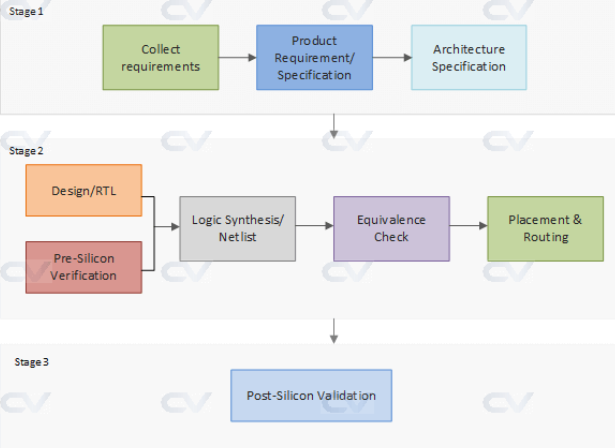
\includegraphics[width=0.75\linewidth]{assets/asic-design-flow.png}
    \caption{ASIC design flow}
    \label{fig:enter-label}
\end{figure}
\begin{table}[H]
    \centering
    \renewcommand{\arraystretch}{1.3} % Tăng khoảng cách giữa các dòng
    \begin{tabular}{|c|p{4cm}|p{5cm}|p{4cm}|}
        \hline
        \textbf{Giai đoạn} & \textbf{Tên Giai Đoạn} & \textbf{Mục tiêu chính} & \textbf{Kết quả đầu ra} \\
        \hline
        1 & Phân tích yêu cầu (Requirement Analysis) & Thu thập yêu cầu, ước lượng thị trường và tài nguyên dự án & Tài liệu đặc tả yêu cầu (System Requirement Spec) \\
        \hline
        2 & Thiết kế kiến trúc (Architecture Design) & Đề xuất kiến trúc tổng thể: PEs, bộ nhớ, giao tiếp, luồng dữ liệu & Tài liệu kiến trúc, sơ đồ khối chức năng \\
        \hline
        3 & Thiết kế RTL (RTL Design) & Mô tả chức năng logic bằng Verilog/VHDL & Mã RTL hoàn chỉnh \\
        \hline
        4 & Mô phỏng chức năng (Functional Simulation) & Kiểm tra tính đúng đắn của mã RTL trước tổng hợp & Kết quả mô phỏng, xác minh logic \\
        \hline
        5 & Tổng hợp (Logic Synthesis) & Biến mã RTL thành sơ đồ mạch logic sử dụng thư viện chuẩn & Gate-level netlist \\
        \hline
        6 & Phân tích thời gian tĩnh (Static Timing Analysis) & Đảm bảo tín hiệu truyền đúng thời gian yêu cầu & Báo cáo timing (setup/hold) \\
        \hline
        7 & Thiết kế vật lý (Physical Design) & Chuyển netlist thành layout vật lý: floorplan, place, route & Layout GDSII, DRC/LVS clean \\
        \hline
        8 & Mô phỏng hậu bố trí (Post-Layout Simulation) & Kiểm tra lại chức năng và thời gian sau layout & Mô phỏng chính xác với parasitic \\
        \hline
        9 & Tape-out & Chuẩn bị file để gửi xưởng chế tạo & File GDSII sẵn sàng sản xuất \\
        \hline
        10 & Kiểm thử và đóng gói (Testing \& Packaging) & Kiểm tra chip thật và đóng gói vào sản phẩm & Chip hoàn chỉnh đã được kiểm định \\
        \hline
    \end{tabular}
    \caption{Các giai đoạn trong thiết kế chip}
    \label{tab:chip_design_stages}
\end{table}

\subsubsection{Yếu tố chính}
\textbf{Kiến trúc luồng dữ liệu (Dataflow Architecture)}
\begin{itemize}
    \item Các chip AI sử dụng các luồng dữ liệu chuyên biệt như mạng systolic hoặc kiến trúc không gian để tối đa hóa tính song song và khả năng tái sử dụng dữ liệu.
    \item Ví dụ: TPU của Google sử dụng mạng systolic để thực hiện các phép nhân ma trận.
\end{itemize}

\textbf{Tối ưu hóa hệ thống bộ nhớ (Memory Hierarchy Optimization)}
\begin{itemize}
    \item Băng thông bộ nhớ và thời gian truy cập là những điểm nghẽn chính trong hiệu suất.
    \item ASICs tối ưu hóa bộ nhớ trên chip (SRAM) và khả năng lưu trữ cục bộ dữ liệu nhằm giảm thiểu việc truy cập bộ nhớ ngoài (DRAM).
\end{itemize}

\textbf{Các phần tử xử lý (Processing Elements - PEs)}
\begin{itemize}
    \item Các mảng PEs thực hiện các phép nhân-tích lũy (MAC), là cốt lõi trong tính toán mạng nơ-ron.
    \item Số lượng và cách sắp xếp các PE ảnh hưởng đến thông lượng và diện tích chip.
\end{itemize}

\textbf{Khả năng mở rộng và tính linh hoạt (Scalability and Flexibility)}
\begin{itemize}
    \item Mặc dù ASICs được thiết kế cho một nhiệm vụ cụ thể, một số chip AI vẫn hỗ trợ mức độ linh hoạt nhất định (ví dụ: hỗ trợ nhiều loại lớp trong mạng nơ-ron).
    \item Có thể bao gồm các tập lệnh tùy chỉnh hoặc khả năng lập trình hạn chế.
\end{itemize}

\textbf{Hiệu suất năng lượng (Power Efficiency)}
\begin{itemize}
    \item Thiết kế tập trung vào việc giảm năng lượng tiêu thụ trên mỗi phép toán (pJ/MAC).
    \item Thường sử dụng các kỹ thuật tiết kiệm điện như tắt nguồn từng phần (power gating) và tắt xung nhịp (clock gating).
\end{itemize}

\textbf{Giao diện và tích hợp (Interface \& Integration)}
\begin{itemize}
    \item ASICs thường được tích hợp vào các hệ thống SoC (System on Chip) lớn hơn.
    \item Bao gồm các giao diện như PCIe, HBM hoặc mạng trên chip (NoC – Network-on-Chip) để giao tiếp dữ liệu.
\end{itemize}

\subsection{Hiệu suất và Năng lượng của ASIC}
\subsubsection{Hiệu suất}
ASIC được thiết kế chuyên biệt cho các tác vụ AI, tối ưu hóa ở cấp độ phần cứng, mang lại hiệu suất cao hơn đáng kể so với CPU và GPU:
TPU đạt 92 TOPS (Tera Operations Per Second) ở độ chính xác 8-bit, gấp 15–30 lần hiệu suất của GPU NVIDIA K80 và CPU Intel Haswell trong cùng workload (Bảng 2, 6).
\begin{figure}
    \centering
    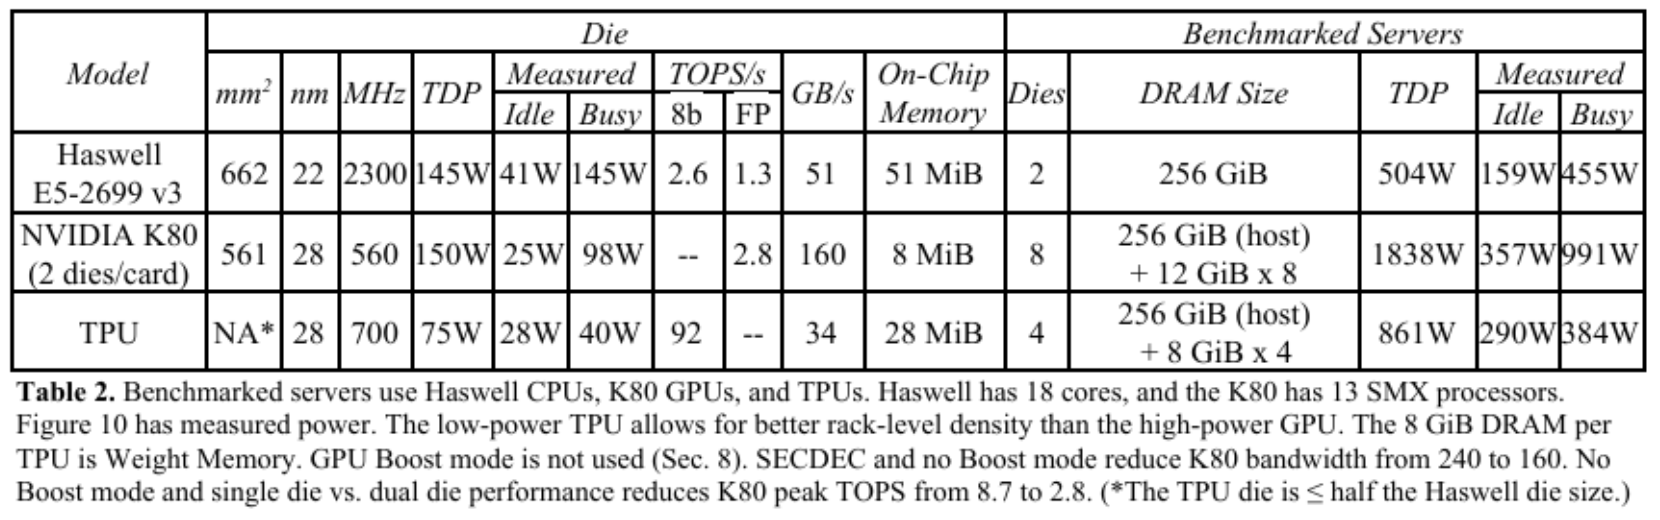
\includegraphics[width=1\linewidth]{assets/table-asic-1.png}
    \caption{Trích tài liệu}
    \label{fig:enter-label}
\end{figure}
\begin{figure}
    \centering
    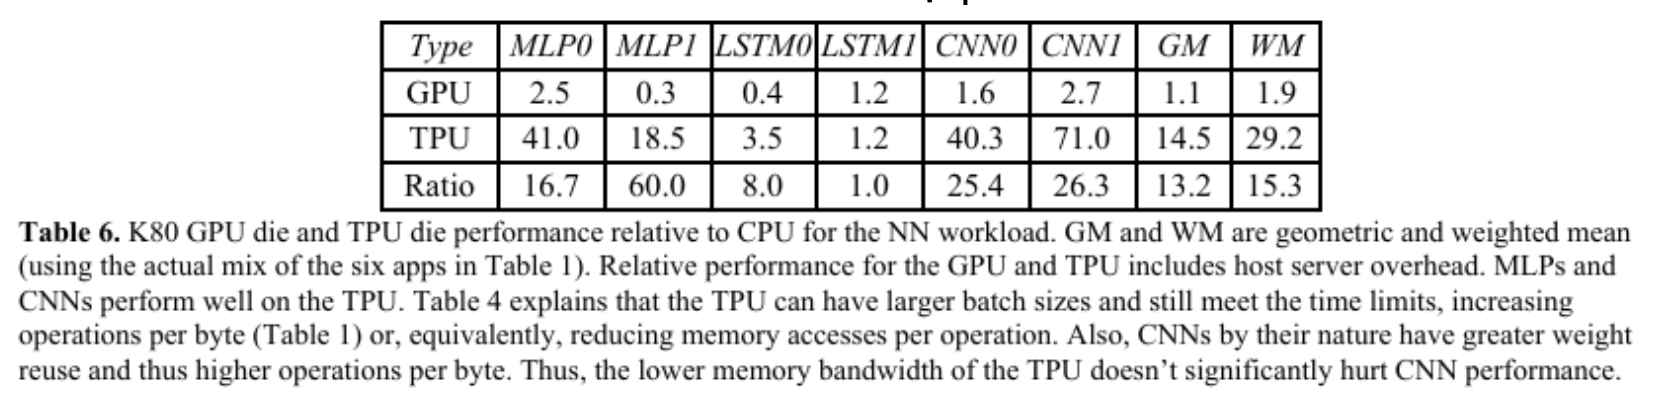
\includegraphics[width=1\linewidth]{assets/table-asic-2.png}
    \caption{Trích tài liệu}
    \label{fig:enter-label}
\end{figure}

Ví dụ: Ứng dụng MLP0 chạy nhanh hơn 41 lần trên TPU so với CPU và 16.7 lần so với GPU (Bảng 6).

Kiến trúc systolic
	Ma trận MAC (Multiply-Accumulate) 256x256 xử lý song song 65,536 phép tính/chu kỳ, giảm độ trễ và tăng thông lượng.

\begin{figure}
    \centering
    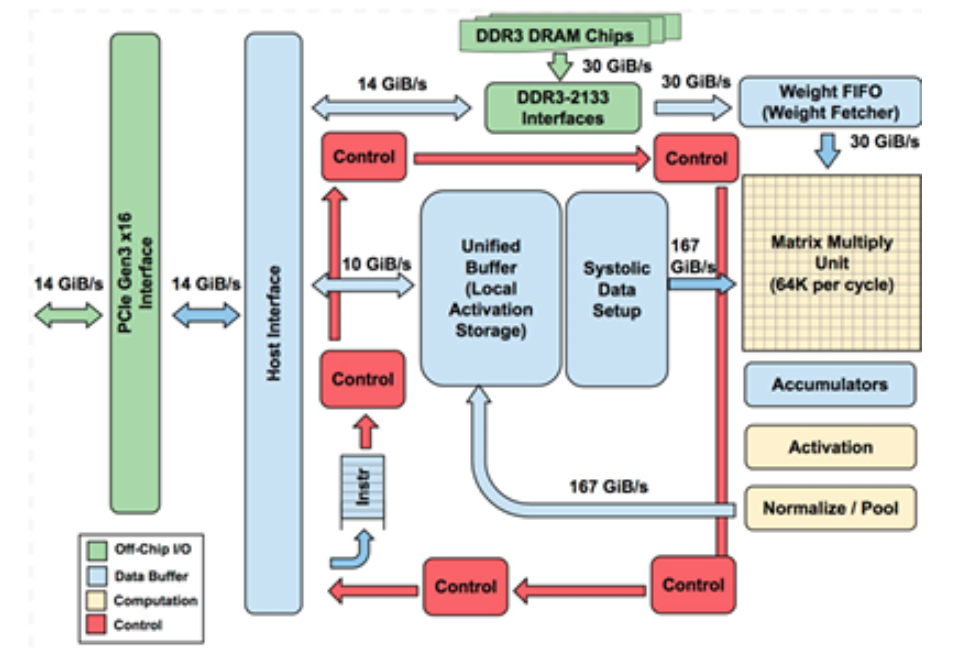
\includegraphics[width=1\linewidth]{assets/tbu-block-diagram.png}
    \caption{TPU Block Diagram. The main computation part is the yellow Matrix Multiply unit in the upper right hand corner. Its input are the blue Weight FIFO and the blue Unified Buffer (UB) and its output is the blue Accumulators (Acc). The yellow Activation Unit performs the nonlinear functions on the Acc. which go to the UB.}
    \label{fig:enter-label}
\end{figure}

\begin{figure}
    \centering
    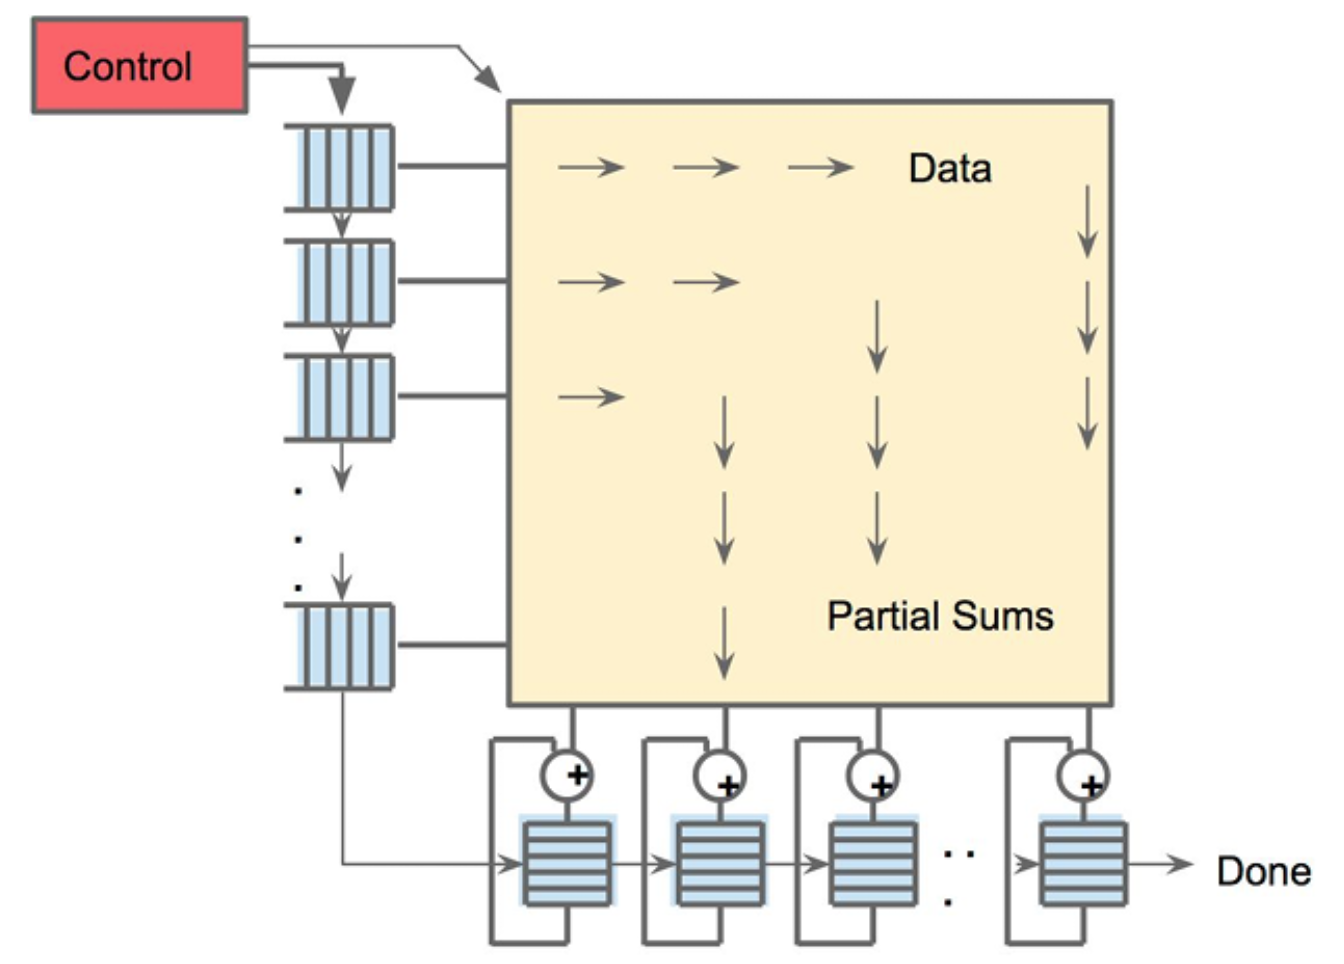
\includegraphics[width=0.75\linewidth]{assets/asic-f4.png}
    \caption{Systolic data flow of the Matrix Multiply Unit. Software has the illusion that each 256B input is read at once, and they instantly update one location of each of 256 accumulator RAMs.}
    \label{fig:enter-label}
\end{figure}
Bộ nhớ on-chip (28 MiB) giảm truy xuất DRAM, tăng operational intensity.

\begin{figure}
    \centering
    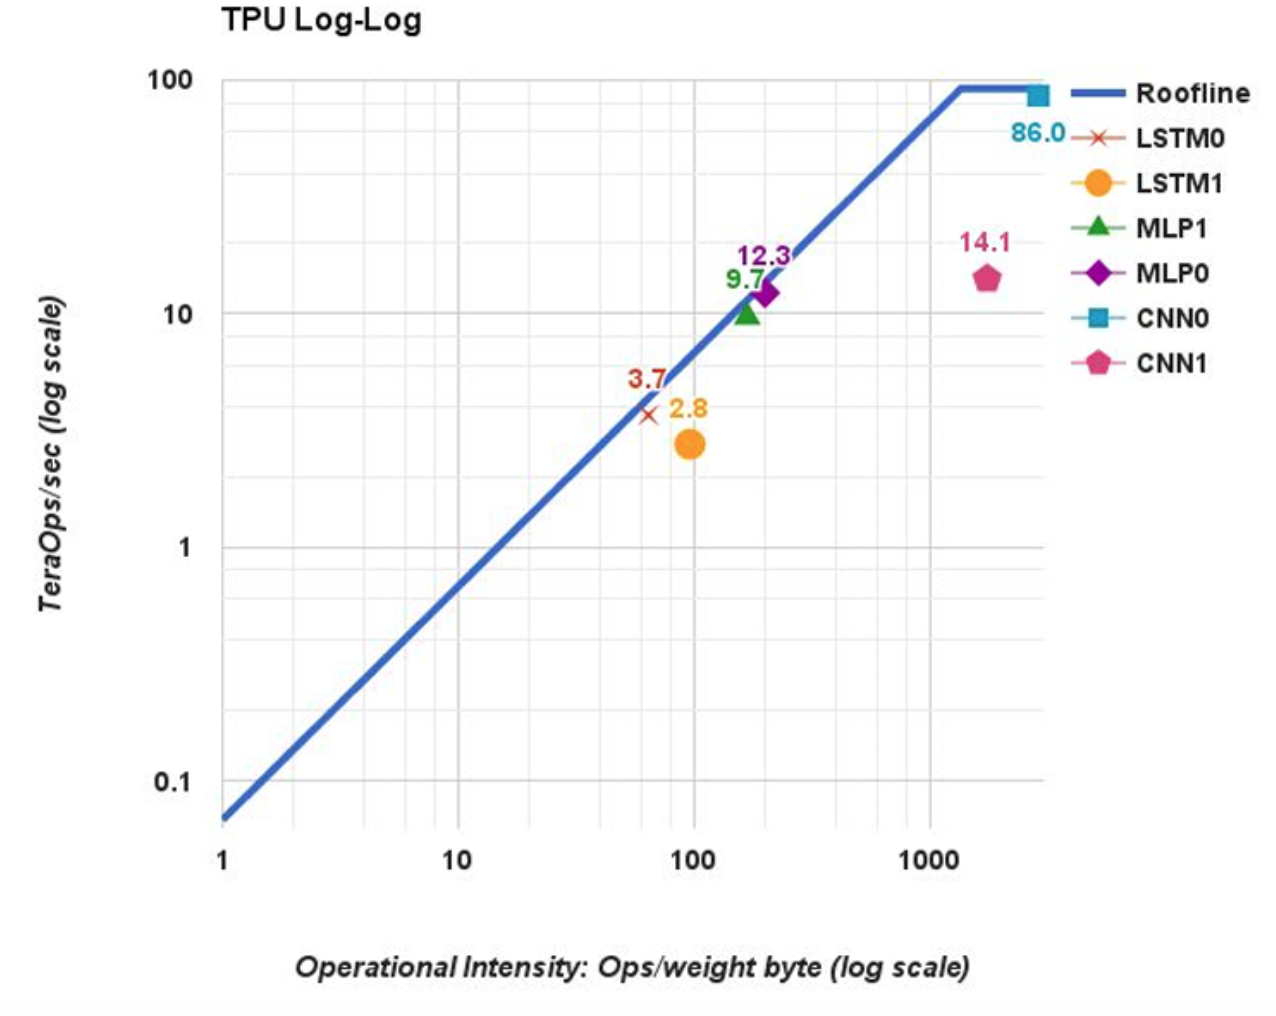
\includegraphics[width=0.75\linewidth]{asic-f5.png}
    \caption{TPU (die) roofline. Its ridge point is far to the right at 1350 operations per byte of weight memory fetched}
    \label{fig:enter-label}
\end{figure}

\textbf{Yếu Tố Then Chốt Tăng Hiệu Suất:}
\begin{itemize}
    \item Tối ưu hóa bộ nhớ:
    Unified Buffer (24 MiB) và Weight FIFO giảm latency khi tải trọng số từ DRAM.
    \item Systolic data flow loại bỏ truy xuất dữ liệu dư thừa, tiết kiệm năng lượng (Hình 4).
    \item Định dạng dữ liệu 8-bit: Giảm 6x năng lượng và 6x diện tích so với phép tính 16-bit dấu phẩy động.
    \item Phù hợp với suy luận AI, duy trì độ chính xác đủ cao.
\end{itemize}
\subsubsection{Năng lượng}
\textbf{Power Components:}
\begin{equation}
    P = P_{DY} + P_{SC} + P_{LK} \quad \text{(dynamic, short-circuit, leakage)}
\end{equation}
\textbf{Optimization Techniques:}
\begin{itemize}
    \item Low-voltage standard cell libraries
    \item Power gating
    \item Clock gating
    \item Asynchronous design
\end{itemize}

\subsection{Ứng dụng công nghệ của ASIC trong mạng neural thần kinh}
\subsubsection{Giới thiệu}
Các mạch tích hợp chuyên dụng (ASIC) đóng vai trò quan trọng trong việc tối ưu hóa hiệu suất và tiêu thụ năng lượng của hệ thống mạng neural, đặc biệt khi tích hợp với công nghệ bộ nhớ flash. FNSim, một công cụ mô phỏng đa năng do Zhang(xem hình 4.1) phát triển, minh họa rõ nét cách tiếp cận thiết kế đồng bộ giữa thiết bị, mạch và thuật toán (device-circuit-algorithm codesign) để đánh giá hệ thống neural dựa trên flash. Bài viết phân tích cấu trúc, nguyên lý hoạt động và ứng dụng của ASIC trong mạng neural thông qua nghiên cứu FNSim.

\subsubsection{Kiến trúc hệ thống FNSim}
ASIC là thành phần tính toán mạng trong hệ thống FNSim, được kết hợp hai thành phần chính:
\textbf{Synapse dựa trên mảng NOR flash:} Lưu trữ trọng số của mạng nơ-ron.
\textbf{Mạch ngoại vi CMOS neuron:} Xử lý tín hiệu đầu vào/đầu ra và thực hiện phép tính tích chập (convolution).

\begin{figure}[H]
    \centering
    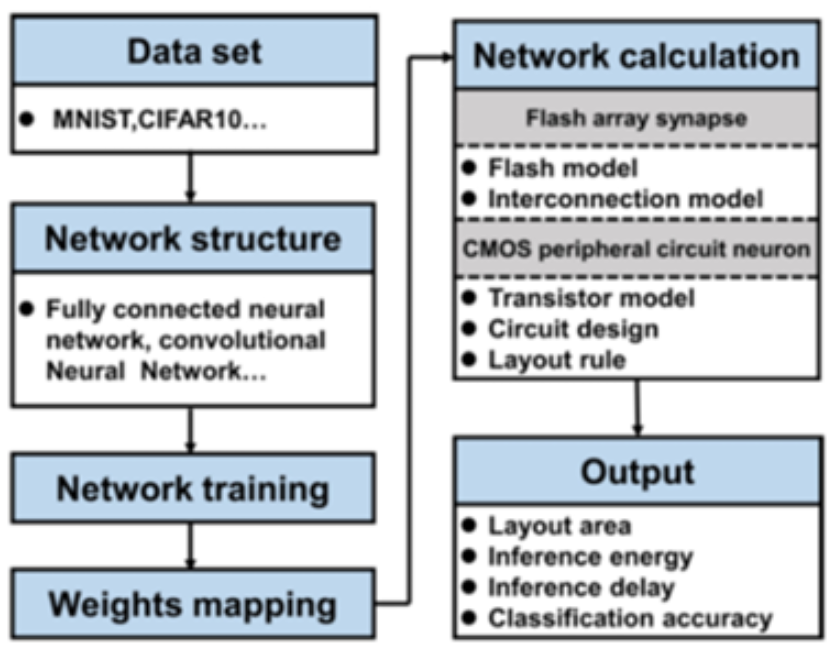
\includegraphics[width=0.75\linewidth]{assets/asic-f6.png}
    \caption{The structure of FNSim}
    \label{fig:enter-label}
\end{figure}

\paragraph{Mạch Ngoại vi CMOS} \leavevmode\\
Mỗi synapse sử dụng hai ô flash để biểu diễn trọng số dương/âm.
Điện áp Word Line (WL) được chuyển đổi từ pixel đầu vào. Khi WL = 0, điện trở của ô flash chuyển sang trạng thái cắt, ngăn dòng điện.
Source Line (SL) kết nối với nguồn điện áp điều khiển, tạo dòng điện tổng hợp qua Bit Line (BL).

\begin{figure}[H]
    \centering
    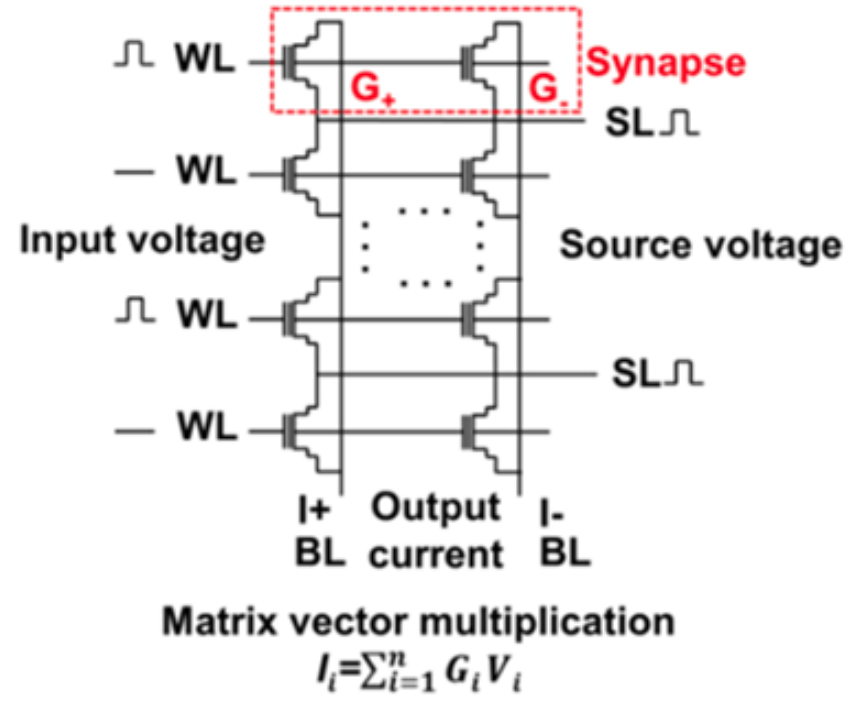
\includegraphics[width=0.5\linewidth]{assets/asic-f7.png}
    \caption{The CMOS neuron peripheral circuit}
    \label{fig:enter-label}
\end{figure}
\paragraph{Synapse Mảng Flash NOR} \leavevmode\\

\begin{figure}
    \centering
    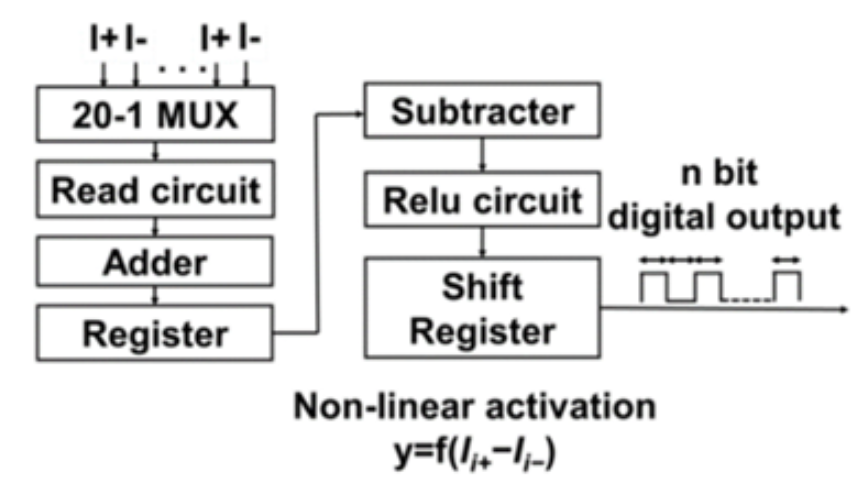
\includegraphics[width=0.5\linewidth]{assets/asic-8.png}
    \caption{The architecture of NOR flash array synapse}
    \label{fig:enter-label}
\end{figure}

\subsection{Các thách thức}
\subsubsection{Chi phí thiết kế và sản xuất cao}
Application-Specific Integrated Circuits (ASICs) đòi hỏi khoản đầu tư lớn vào nghiên cứu, thiết kế và chế tạo. Khác với các bộ xử lý đa năng, ASICs được tùy chỉnh cho các nhiệm vụ cụ thể, yêu cầu quy trình sản xuất độc nhất, làm gia tăng chi phí.
Ví dụ: Google Cloud pricing [1]
Google không công bố chi phí của GPUs và TPUs trong báo cáo tài chính của mình.
Theo nghiên cứu của Omdia, chi phí mua sắm TPUs của Google ước tính nằm trong khoảng từ 6 tỷ đến 9 tỷ USD vào năm 2024.
Google mua hàng ngàn GPUs từ NVIDIA mỗi năm.
Tuy nhiên, chúng ta có thể dựa vào mức giá của GPUs và TPUs mà Google cung cấp trên nền tảng Google Cloud Platform.
\begin{figure}[H]
    \centering
    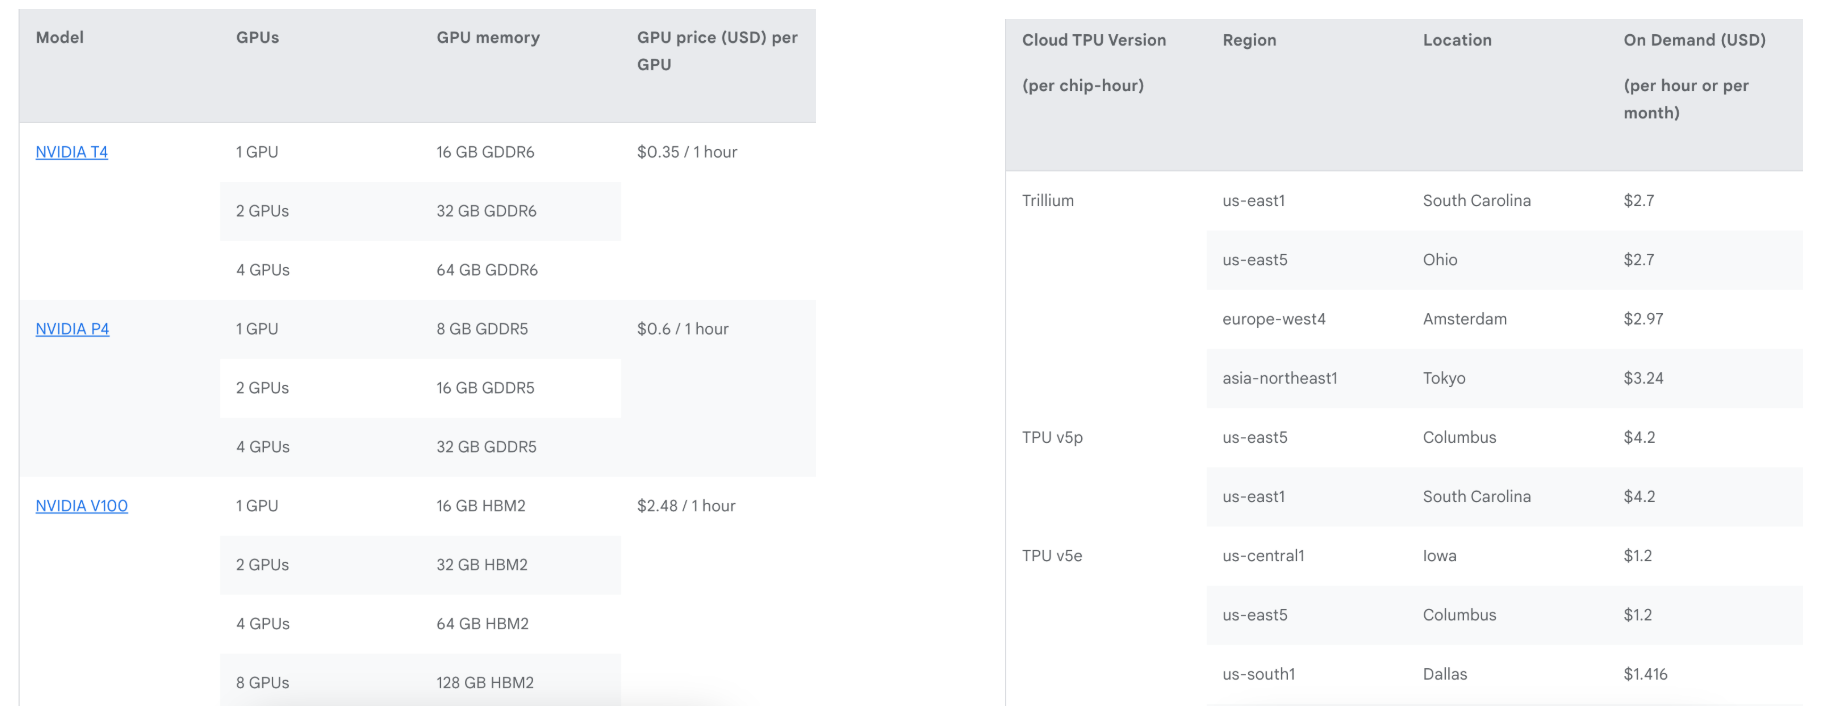
\includegraphics[width=0.75\linewidth]{assets/asic-gg.png}
    \caption{Giá Google’s GPU (ảnh trái - \href{https://cloud.google.com/compute/gpus-pricing?hl=en}{Source}) và TPU (ảnh phải - \href{https://cloud.google.com/tpu/pricing?hl=en}{Source}}
    \label{fig:enter-label}
\end{figure}

Bên cạnh đó, Kaggle - một cộng đồng AI nổi tiếng - cung cấp hạn mức miễn phí là 30 giờ/tuần/người dùng cho GPU và chỉ 20 giờ/tuần/người dùng cho TPU.
\begin{figure}[H]
    \centering
    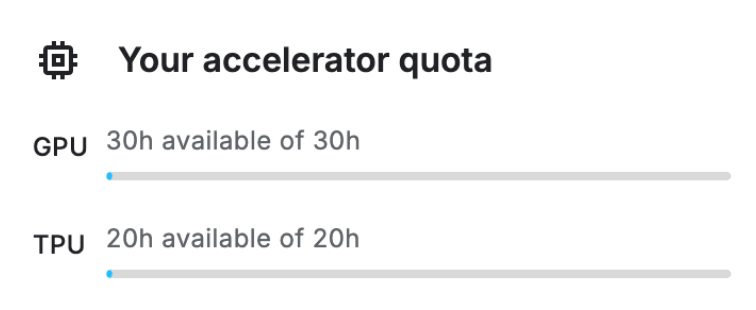
\includegraphics[width=0.75\linewidth]{assets/asic-kg.png}
    \caption{Kaggle quota}
    \label{fig:enter-label}
\end{figure}
\subsubsection{Khả năng linh hoạt hạn chế}
ASICs được thiết kế cho các ứng dụng cụ thể, khiến chúng kém thích ứng với các thay đổi về công nghệ và nhu cầu thị trường, dẫn đến nguy cơ mất doanh thu nếu nhu cầu thị trường thay đổi đột ngột.
Ví dụ: Công ty Bitmain
\begin{itemize}
    \item Theo \href{https://www.coindesk.com/markets/2018/09/27/bitmain-by-the-numbers-an-inside-look-at-a-bitcoin-mining-empire}{báo cáo của CoinDesk}, Bitmain, công ty thiết bị khai thác tiền điện tử lớn nhất thế giới, đã thua lỗ 500 triệu USD trong quý 3 năm 2018 do cái gọi là “Crypto Winter”.  
    \item Thuật ngữ “Crypto Winter” đề cập đến giai đoạn khi giá Bitcoin giảm mạnh trong thời gian ngắn và sau đó duy trì ở mức thấp trong thời gian dài (tức là kéo dài nhiều tháng).  
    \item Khi giá Bitcoin giảm, một số thợ đào mất niềm tin vào giá trị của Bitcoin và ngừng mua các máy khai thác mới, vốn sử dụng chip ASIC được thiết kế riêng cho mục đích này. Do các chip này có tính linh hoạt hạn chế và không thể tái sử dụng cho các mục đích khác, công ty không thể bán được sản phẩm mới, dẫn đến mất doanh thu.

\end{itemize}

\subsubsection{Phụ thuộc vào chuỗi cung ứng bán dẫn}
Việc sản xuất ASIC phụ thuộc vào chuỗi cung ứng phức tạp, bao gồm chế tạo bán dẫn, thu mua vật liệu và hậu cần. Gián đoạn toàn cầu có thể ảnh hưởng nghiêm trọng đến sản xuất và giá cả. 
\begin{itemize}
    \item Cả ba loại chip - ASIC, GPU và FPGA - đều phụ thuộc vào chuỗi cung ứng toàn cầu, nhưng ASIC có mức độ phụ thuộc cao nhất do yêu cầu các nhà máy tiên tiến với các nút tiến trình hiện đại (3nm–7nm), trong khi trên thế giới chỉ có một vài nhà máy như TSMC, Samsung, v.v. Thêm vào đó, thiết kế ASIC không thể thay đổi sau khi sản xuất.
    \item Do đó, bất kỳ sự chậm trễ hoặc gián đoạn nào trong chuỗi cung ứng đều có thể gây thiệt hại lớn cho quá trình phát triển chip.    
\end{itemize}
Một vài ví dụ:
\begin{itemize}
    \item \href{https://en.wikipedia.org/wiki/2020%E2%80%932023_global_chip_shortage}{2020–2023 global chip shortage}
    \item \href{https://www.theregister.com/2024/07/18/tsmc_ceo_predicts_ai_chip/}{AI chip shortage through 2025 prediction from TSMC boss}
\end{itemize}

\begin{figure}[H]
    \centering
    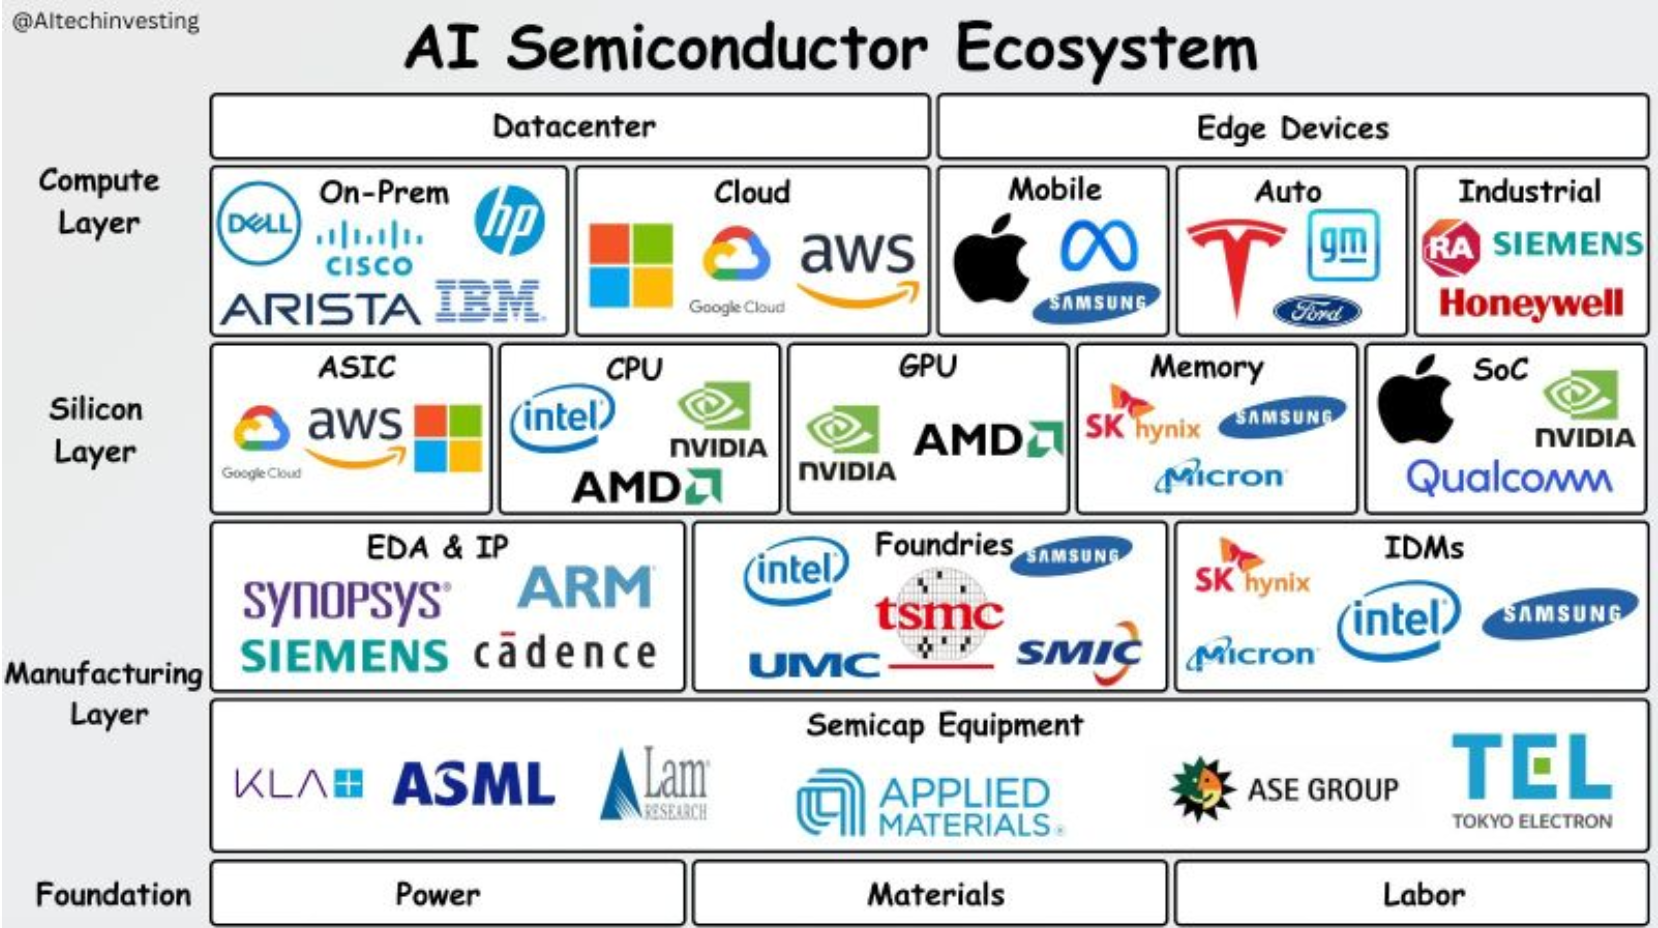
\includegraphics[width=0.75\linewidth]{assets/ai-semiconductor.png}
    \caption{Hệ sinh thái các công ty liên quan đến AI ASIC chips (\href{https://techovedas.com/what-are-major-players-in-ai-ecosystem/}{Nguồn})}
    \label{fig:enter-label}
\end{figure}

\textbf{Kết luận}
Những thách thức trong phát triển ASIC bao gồm chi phí đầu tư ban đầu cao, dễ bị ảnh hưởng bởi chuỗi cung ứng và tính linh hoạt hạn chế. Mặc dù gặp nhiều trở ngại, ASIC vẫn đóng vai trò quan trọng trong các ứng dụng hiệu năng cao như tăng tốc AI, khai thác tiền điện tử và hạ tầng viễn thông. Việc giải quyết những thách thức này đòi hỏi cải tiến trong phương pháp thiết kế, tăng cường khả năng phục hồi chuỗi cung ứng và phát triển công nghệ chế tạo.

\subsection{Xu hướng}
\subsubsection{Tiếp tục thu nhỏ kích thước và tối ưu hóa hiệu suất}
Khi công nghệ bán dẫn phát triển, ASIC tiếp tục hưởng lợi từ các nút xử lý nhỏ hơn, mang lại hiệu suất cao hơn và tiết kiệm năng lượng hơn. Việc giới thiệu các nút xử lý 3nm và sắp tới là 2nm bởi các xưởng đúc lớn như TSMC và Samsung được kỳ vọng sẽ cải thiện mật độ bóng bán dẫn và giảm tiêu thụ điện năng.  

Ví dụ: TSMC đã bắt đầu sản xuất hàng loạt ASIC 3nm và có kế hoạch ra mắt công nghệ 2nm vào năm 2025.
\subsubsection{ASIC cho tăng tốc AI và Machine Learning}
Sự mở rộng nhanh chóng của khối lượng công việc AI và machine learning đã dẫn đến nhu cầu gia tăng đối với các ASIC chuyên dụng được thiết kế cho suy luận và huấn luyện deep learning. Các chip này được thiết kế để tối ưu hóa phép nhân ma trận và các phép toán tensor, giúp giảm độ trễ và cải thiện hiệu suất.

Ví dụ:
\begin{itemize}
    \item Google TPU: Google đã liên tục cải thiện dòng TPU của mình, với phiên bản mới nhất v5 mang lại sức mạnh xử lý cao hơn và tiêu thụ điện năng thấp hơn.  
    \item Tesla Dojo: Tesla đang phát triển siêu máy tính Dojo, tích hợp các ASIC tùy chỉnh để huấn luyện mô hình AI được sử dụng trong hệ thống lái tự động (Nguồn: Tesla’s D1 chips).
\end{itemize}
\subsubsection{Mở rộng trong các lĩnh vực khác}
\begin{itemize}
    \item Mạng 6G: Các ASIC được thiết kế cho mạng 5G và tương lai 6G giúp giảm độ trễ và tăng tốc độ xử lý dữ liệu, cải thiện kết nối và giảm tiêu thụ điện năng.  
    \item Điện toán biên và IoT: Khi nhu cầu về điện toán biên và các ứng dụng Internet of Things (IoT) tăng cao, các ASIC được thiết kế để xử lý trên thiết bị một cách hiệu quả. Những chip này cho phép xử lý dữ liệu theo thời gian thực, giảm sự phụ thuộc vào điện toán đám mây và cải thiện tốc độ phản hồi.  
    \item Tiền điện tử và Công nghệ Blockchain: ASIC vẫn là giải pháp phần cứng chủ đạo cho khai thác tiền điện tử nhờ hiệu suất cao và sức mạnh băm. Tuy nhiên, sự thay đổi trong các giao thức blockchain và mối lo ngại về năng lượng đang thúc đẩy việc phát triển các giải pháp khai thác bền vững hơn.
\end{itemize}
\subsubsection{Cải thiện tính linh hoạt}
Một Google TPU v5p Pod bao gồm 8.960 chip được kết nối với nhau bằng các liên kết tốc độ cao có thể cấu hình lại, hoạt động hiệu quả với nhiều loại mô hình khác nhau (CNN, Transformer, ...).

\subsection{Neural Processing Unit (NPU)}
\subsubsection{Mô tả}
Neural Processing Units (NPUs) là các bộ xử lý chuyên dụng được thiết kế tối ưu cho các tác vụ liên quan đến trí tuệ nhân tạo (AI) như nhận diện hình ảnh, xử lý giọng nói, và dự đoán thời gian thực. NPUs thường được tích hợp trong các thiết bị di động, IoT (Internet of Things), và các thiết bị biên (edge devices) như điện thoại, đồng hồ thông minh, nhằm tăng cường hiệu suất xử lý AI ngay trên thiết bị mà không cần gửi dữ liệu về đám mây. Điều này giúp giảm độ trễ, tăng tốc độ phản hồi, và bảo vệ tính riêng tư của người dùng.

\subsubsection{Kiến trúc của NPUs}
NPUs được thiết kế để tối ưu hóa các phép toán tensor và ma trận, vốn là cốt lõi của các mô hình học sâu. Một số đặc điểm chính của kiến trúc NPU bao gồm:

\begin{itemize}
    \item \textbf{MAC (Multiply-Accumulate Units)}\\
    NPUs được trang bị các đơn vị MAC (nhân và cộng) giúp thực hiện các phép tính số học nhanh chóng và hiệu quả, đặc biệt là các phép nhân ma trận và tích chập (convolution).



\item \textbf{Bộ nhớ chuyên dụng (Dedicated Memory)}\\
NPUs sử dụng các bộ đệm (buffer) tốc độ cao để lưu trữ tạm thời các tensor trong quá trình xử lý, giảm thiểu độ trễ khi truy xuất dữ liệu.

\item \textbf{Pipelining và Parallelism}\\
Kiến trúc NPU được tối ưu cho pipelining và parallel processing, cho phép thực hiện nhiều tác vụ AI song song để tăng tốc độ xử lý.

Nếu GPU được trang bị CUDA cores đa nhân hỗ trợ tốt parallel processing thì NPU được trang bị \textbf{PE (Processing Engine)} để tối ưu.
    \begin{itemize}
        \item CUDA Cores
        \begin{itemize}
        \item Được thiết kế để xử lý đồng thời hàng nghìn luồng dữ liệu, phù hợp với các tác vụ tổng quát như đồ họa và học sâu.
        \item Hoạt động với độ chính xác cao (FP32, FP64), hỗ trợ tốt cho huấn luyện mô hình AI nhưng tiêu tốn nhiều năng lượng.
        \end{itemize}
        
        \item{Processing Engine (PE)}
        \begin{itemize}
        \item Được tối ưu hóa cho các tác vụ AI chuyên biệt như suy luận và tích chập.
        \item Hiệu quả về năng lượng và tốc độ khi xử lý dữ liệu tensor và ma trận, phù hợp cho các thiết bị di động.
        \end{itemize}
    \end{itemize}
\end{itemize}
\subsubsection{Lợi ích của việc sử dụng NPUs}
\begin{itemize}
    \item \textbf{Tăng tốc xử lý AI trên thiết bị (On-device AI):} NPUs giúp tăng tốc độ xử lý các mô hình AI ngay trên thiết bị di động, hỗ trợ các ứng dụng như nhận diện khuôn mặt, phân loại hình ảnh và xử lý ngôn ngữ tự nhiên trong thời gian thực.
    
    \item \textbf{Giảm độ trễ (Low Latency):} Thay vì gửi dữ liệu lên đám mây để xử lý, NPUs thực hiện tính toán trực tiếp trên thiết bị, giảm độ trễ đáng kể. Điều này đặc biệt quan trọng với các ứng dụng yêu cầu phản hồi tức thời như thực tế ảo tăng cường (AR) hay điều khiển bằng giọng nói.
    
    \item \textbf{Tiết kiệm năng lượng (Power Efficiency):} Được thiết kế để tiêu thụ ít điện năng hơn so với CPU và GPU truyền thống, NPUs rất phù hợp cho các thiết bị di động và IoT có giới hạn về pin. Các mô hình AI tối ưu hóa (FP32 – FP16) kết hợp với kiến trúc tính toán hiệu quả giúp giảm mức tiêu thụ năng lượng đáng kể.
    
    \item \textbf{Bảo vệ quyền riêng tư (Privacy):} Dữ liệu được xử lý trực tiếp trên thiết bị thay vì gửi ra bên ngoài, giúp bảo vệ thông tin cá nhân và tăng cường bảo mật.
\end{itemize}

\subsubsection{Ứng dụng thực tế của NPUs}
\begin{itemize}
    \item \textbf{Nhận diện hình ảnh và video (Image and Video Recognition):} NPUs trên smartphone giúp nâng cao chất lượng ảnh và video bằng cách áp dụng công nghệ AI như HDR (High Dynamic Range), chế độ ban đêm, và nhận diện cảnh theo thời gian thực. \\
    \textit{Ví dụ:} Apple Neural Engine trên iPhone cải thiện hiệu suất xử lý ảnh và hỗ trợ nhận diện khuôn mặt (Face ID).

    \item \textbf{Xử lý giọng nói và ngôn ngữ tự nhiên (Voice and Natural Language Processing - NLP):} Các thiết bị như loa thông minh và tai nghe không dây sử dụng NPUs để nâng cao khả năng nhận diện giọng nói, dịch thuật và xử lý lệnh thoại. \\
    \textit{Ví dụ:} Google Pixel tích hợp NPU để cải thiện tốc độ và độ chính xác của Google Assistant và dịch thuật thời gian thực.

    \item \textbf{AI trên các thiết bị biên và IoT (Edge AI):} NPUs trong thiết bị IoT như camera an ninh, cảm biến thông minh và robot tự động giúp xử lý dữ liệu tại chỗ, giảm nhu cầu truyền dữ liệu về máy chủ. \\
    \textit{Ví dụ:} Huawei Ascend AI Processor trang bị NPU để hỗ trợ xử lý AI trên các hệ thống giám sát và nhà thông minh.
\end{itemize}

\subsubsection{Các NPU tiêu biểu}
\begin{itemize}
    \item \textbf{Apple Neural Engine (ANE):} Được tích hợp trong các dòng iPhone và iPad mới nhất, ANE có khả năng thực hiện lên đến 11 nghìn tỷ phép toán mỗi giây (11 TOPS), giúp tăng tốc xử lý AI cho các tác vụ như nhận diện khuôn mặt và xử lý hình ảnh.
    
    \item \textbf{Huawei Kirin NPU:} Tích hợp trong vi xử lý Kirin của Huawei, NPU này được tối ưu hóa cho các tác vụ AI như nhận diện vật thể, xử lý ngôn ngữ và chụp ảnh thông minh với AI.
    
    \item \textbf{Samsung Exynos NPU:} Được trang bị trong chip Exynos của Samsung, giúp tăng tốc xử lý AI cho ứng dụng như tối ưu hóa hình ảnh, nhận diện cảnh và thực tế tăng cường (AR).
    
    \item \textbf{Google Tensor SoC:} Sử dụng trên dòng Google Pixel, NPU này nâng cao khả năng xử lý ảnh và hỗ trợ các tính năng AI liên quan đến giọng nói.
\end{itemize}

\subsubsection{Thách thức và hạn chế}
\begin{itemize}
    \item \textbf{Tối ưu hóa phần mềm:} Việc khai thác tối đa hiệu suất của NPU đòi hỏi các mô hình AI phải được tối ưu hóa theo phần cứng cụ thể, điều này có thể phức tạp và mất thời gian.
    
    \item \textbf{Khả năng tương thích:} Một số mô hình AI có thể không hoạt động tốt trên NPU do hạn chế về định dạng dữ liệu hoặc yêu cầu thuật toán đặc thù.
    
    \item \textbf{Chi phí phát triển:} Việc tích hợp NPU vào sản phẩm đòi hỏi chi phí cao và cần đội ngũ kỹ thuật có chuyên môn sâu.
\end{itemize}

%%%%%%%%%%%%%%%%%%%%%%%%%%%
\section{FPGA - Field-Programmable Gate Array}
\subsection{Why reconfigurable computing?}
1.1. Hiệu suất và năng lượng vượt trội của các bộ tăng tốc
\begin{figure}[H]
    \centering
    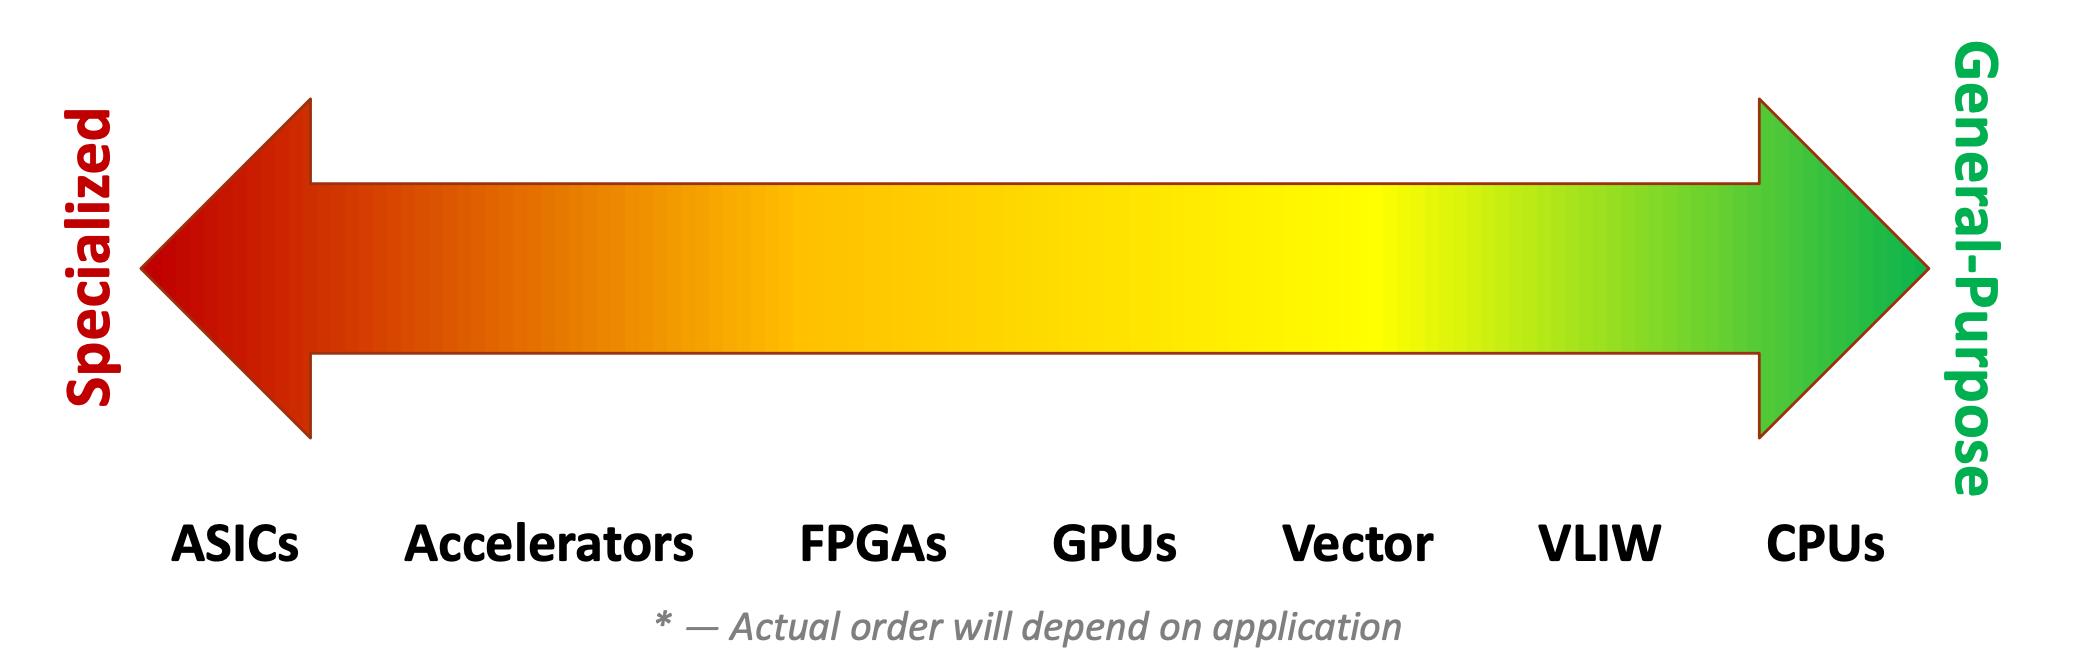
\includegraphics[width=1\linewidth]{assets/phanloai.png}
    \caption{Phân loại phần cứng trên trục Specialized - General-Purpose}
    \label{fig:enter-label}
\end{figure}
ASICs và accelerators mang lại hiệu suất và hiệu quả năng lượng cao, nhưng thiếu tính linh hoạt và tốn kém để phát triển. CPUs và VLIW rất linh hoạt, nhưng không thể cạnh tranh về hiệu suất cho các tác vụ chuyên biệt. FPGAs, nằm ở vị trí trung gian, là một ví dụ điển hình của Reconfigurable Computing—chúng có thể được tái cấu hình để đạt hiệu suất cao cho nhiều loại tác vụ, nhưng vẫn không đạt được hiệu quả năng lượng của ASICs. Mục tiêu của Reconfigurable Computing là tìm một điểm cân bằng trên trục này, nơi chúng ta có thể đạt được hiệu suất gần với ASICs nhưng vẫn giữ được tính linh hoạt của CPUs, mà không cần phát triển phần cứng tùy chỉnh.

\subsection{Giới thiệu về FPGA}
FPGA (\textit{Field Programmable Gate Array}), còn gọi là mảng cổng lập trình được trên hiện trường, là một thiết bị bán dẫn được cấu thành từ các khối logic khả trình (\textit{Programmable Logic Blocks}), các kết nối liên thông (\textit{Interconnects}) linh hoạt và bộ nhớ nội (\textit{on-chip memory}). FPGA cho phép người dùng tái cấu hình và lập trình lại các chức năng phần cứng sau khi sản xuất, điều này giúp FPGA trở nên linh hoạt hơn so với ASIC (mạch tích hợp chuyên dụng), vốn có cấu trúc cố định ngay từ khi sản xuất.

Kiến trúc cơ bản của FPGA bao gồm:
\begin{itemize} [label=-]
    \item \textbf{CLB (Configurable Logic Blocks)}: các khối logic khả trình để thực hiện các chức năng logic tuỳ biến.
    \item \textbf{Interconnects}: mạng liên kết lập trình được dùng để kết nối các CLB với nhau.
    \item \textbf{Bộ nhớ nội (Block RAM)}: lưu trữ dữ liệu trên chip, giảm nhu cầu truy cập bộ nhớ ngoài.
    \item \textbf{Khối DSP (Digital Signal Processing Blocks)}: thực hiện các phép toán phức tạp như nhân, cộng nhanh.
\end{itemize}

\subsubsection{Lịch sử phát triển FPGA:} FPGA được giới thiệu lần đầu tiên bởi hãng Xilinx vào năm 1985 với sản phẩm XC2064. Đây là mạch FPGA thương mại đầu tiên, đánh dấu sự khởi đầu cho một xu hướng công nghệ mới trong lĩnh vực thiết kế điện tử. 

Lịch sử phát triển FPGA trải qua một số giai đoạn chính:
\begin{itemize} [label=-]
    \item \textbf{Thập niên 1980}: FPGA ra đời, chủ yếu dành cho các ứng dụng đơn giản, thay thế các mạch logic riêng lẻ.
    \item \textbf{Thập niên 1990}: FPGA bắt đầu tích hợp bộ nhớ nội và các khối DSP, tăng khả năng tính toán song song và ứng dụng xử lý tín hiệu.
    \item \textbf{Thập niên 2000}: FPGA phát triển mạnh về khả năng tích hợp, tăng số lượng khối logic và mở rộng băng thông giao tiếp, ứng dụng trong viễn thông và mạng.
    \item \textbf{Từ năm 2010 đến nay}: FPGA trở nên phổ biến trong lĩnh vực điện toán hiệu năng cao (HPC), trí tuệ nhân tạo (AI), học máy (Machine Learning) và xử lý dữ liệu lớn (Big Data). Các công ty như Xilinx, Altera (nay thuộc Intel), Lattice Semiconductor dẫn đầu thị trường.
\end{itemize}

\subsubsection{Các ngôn ngữ mô tả phần cứng dùng cho FPGA:}
Quá trình lập trình và tái cấu hình FPGA chủ yếu sử dụng các ngôn ngữ mô tả phần cứng (\textit{Hardware Description Languages} -- HDL), phổ biến nhất là:

\begin{itemize} [label=-]
    \item \textbf{Verilog}: Là ngôn ngữ mô tả phần cứng phổ biến, dễ học, có cú pháp tương tự ngôn ngữ lập trình C, phù hợp với các nhà phát triển có nền tảng lập trình phần mềm.
    \item \textbf{VHDL (Very High-Speed Integrated Circuit Hardware Description Language)}: Có cú pháp chặt chẽ, rõ ràng, thích hợp với các thiết kế đòi hỏi tính chính xác và độ tin cậy cao, phổ biến trong môi trường công nghiệp.
    \item \textbf{SystemVerilog}: Phát triển dựa trên Verilog, hỗ trợ lập trình hướng đối tượng và các tính năng cao cấp hơn, đặc biệt thích hợp cho các dự án lớn và phức tạp.
    \item \textbf{Ngôn ngữ bậc cao và HLS (High-Level Synthesis)}: Gần đây, các công cụ HLS như Vivado HLS (Xilinx), Intel HLS Compiler cho phép lập trình FPGA bằng các ngôn ngữ C, C++, SystemC, giúp đơn giản hoá quá trình thiết kế phần cứng.
\end{itemize}

\subsection{Ứng dụng FPGA qua các năm}
\begin{itemize} [label=-]
    \item \textbf{Classically: ASIC prototyping, Low-volume applications:} \par
    Ban đầu, FPGA được sử dụng chủ yếu cho hai mục đích: ASIC prototyping (tạo mẫu ASIC) và low-volume applications (ứng dụng sản lượng thấp). Trong ASIC prototyping, FPGA được sử dụng để kiểm tra thiết kế phần cứng trước khi sản xuất ASIC, vì việc sửa lỗi trên FPGA rẻ và nhanh hơn nhiều so với sửa ASIC. Ví dụ, một công ty thiết kế ASIC cho xử lý tín hiệu có thể triển khai thiết kế trên FPGA để kiểm tra chức năng, sau đó sản xuất ASIC khi thiết kế đã ổn định. Trong low-volume applications, FPGA được sử dụng cho các sản phẩm có số lượng sản xuất thấp (như thiết bị y tế hoặc quân sự), nơi chi phí thiết kế ASIC không khả thi. Ví dụ, một thiết bị y tế chuyên dụng có thể sử dụng FPGA để xử lý tín hiệu, vì chỉ cần sản xuất vài trăm đơn vị.
    \item \textbf{More recently: “General-purpose acceleration” platform, Widely deployed in datacenter @ Microsoft, Amazon} \par
    Gần đây (tính đến năm 2019), FPGA đã chuyển sang vai trò "general-purpose acceleration" platform (nền tảng tăng tốc đa năng), và được triển khai rộng rãi trong các trung tâm dữ liệu (datacenters) bởi các công ty lớn như Microsoft và Amazon. Trong vai trò này, FPGA được sử dụng để tăng tốc các tác vụ tính toán chuyên biệt, như học sâu, xử lý tìm kiếm, hoặc mã hóa video, trong khi vẫn giữ được tính linh hoạt để tái cấu hình cho các tác vụ khác. Ví dụ, Microsoft sử dụng FPGA trong Azure để tăng tốc các truy vấn tìm kiếm của Bing, đạt hiệu suất cao hơn nhiều so với CPU. Tương tự, Amazon sử dụng FPGA trong AWS (Amazon Web Services) để cung cấp dịch vụ tăng tốc học máy (machine learning acceleration) cho khách hàng, cho phép họ tái cấu hình FPGA để phù hợp với mô hình học máy cụ thể.
    \item \textbf{Why the shift? Slowdown in CPU performance scaling, Cloud operators want to serve a variety of customers (reconfigurability++):} \par
    Lý do cho sự thay đổi này qua hai yếu tố chính. Thứ nhất, "Slowdown in CPU performance scaling" (Sự chậm lại trong việc mở rộng hiệu suất CPU): Theo định luật Moore, hiệu suất CPU từng tăng gấp đôi sau mỗi 18-24 tháng, nhưng từ khoảng năm 2010, sự mở rộng này đã chậm lại do các giới hạn vật lý (như kích thước bóng bán dẫn nhỏ hơn dẫn đến rò rỉ điện và tiêu thụ năng lượng cao). Điều này khiến CPU không còn đáp ứng được nhu cầu tính toán ngày càng tăng, đặc biệt trong các ứng dụng như học sâu hoặc xử lý dữ liệu lớn. FPGA, với khả năng song song hóa phần cứng (hardware parallelism), trở thành một giải pháp thay thế hiệu quả để tăng tốc các tác vụ chuyên biệt. Thứ hai, "Cloud operators want to serve a variety of customers (reconfigurability++)" (Các nhà vận hành đám mây muốn phục vụ nhiều khách hàng khác nhau): Trong các trung tâm dữ liệu, các nhà cung cấp như Microsoft và Amazon cần hỗ trợ nhiều loại ứng dụng khác nhau (tìm kiếm, học máy, mã hóa video, v.v.). Tính tái cấu hình (reconfigurability) của FPGA cho phép họ triển khai một nền tảng phần cứng duy nhất, sau đó tái cấu hình nó để đáp ứng nhu cầu của từng khách hàng, thay vì phải sử dụng nhiều loại ASIC khác nhau.

\end{itemize}

\subsection{Components of an FPGA}
FPGA là một thành phần quan trọng trong lĩnh vực Reconfigurable Computing, nó là một mạch tích hợp có thể lập trình được, cho phép người dùng cấu hình lại logic và kết nối của nó sau khi sản xuất. Vì thế, nó cung cấp sự linh hoạt trong việc lập trình phần cứng để thực hiện các tác vụ cụ thể, đồng thời duy trì khả năng tái cấu hình để thích nghi với nhiều ứng dụng khác nhau.
\begin{figure}[H]
    \centering
    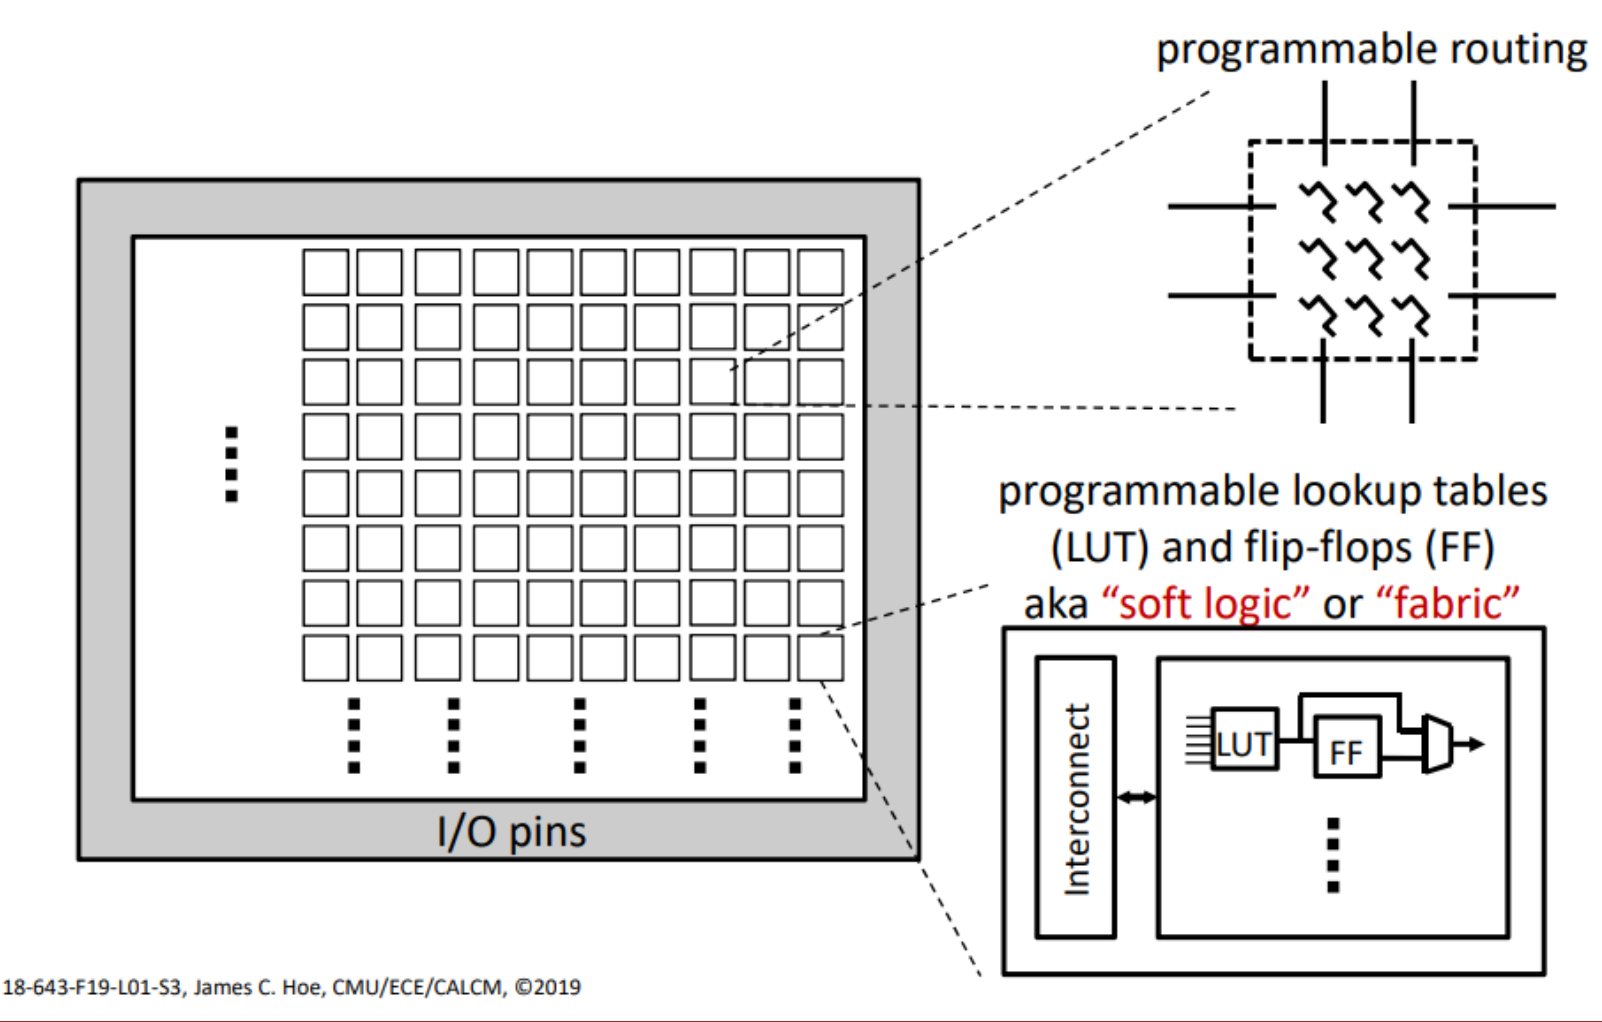
\includegraphics[width=1\linewidth]{assets/fpag.png}
    \caption{FPGA components}
    \label{fig:enter-label}
\end{figure}
Sơ đồ này minh họa các thành phần chính của FPGA, bao gồm:
\begin{itemize}
    \item \textbf{Khối logic (Logic Blocks):} Các ô vuông trong lưới đại diện cho các khối logic, còn được gọi là \textbf{Configurable Logic Blocks} (CLBs) hoặc \textbf{Logic Elements} (LEs), tùy thuộc vào nhà sản xuất (như Xilinx hoặc Intel). Mỗi khối logic là một đơn vị cơ bản có thể được lập trình để thực hiện các hàm logic, chẳng hạn như AND, OR, XOR, hoặc các hàm phức tạp hơn. Các khối logic này được sắp xếp thành một mảng 2D, với các hàng và cột được kết nối bởi một mạng định tuyến (routing network).
    \item  \textbf{Mạng định tuyến có thể lập trình (Programmable Routing):} Các đường ngang và dọc giữa các khối logic đại diện cho \textbf{interconnect} (mạng kết nối), được minh họa chi tiết hơn ở phần bên phải của hình ảnh. Mạng định tuyến này bao gồm các đường dây (wires) và các điểm chuyển mạch (switches) có thể lập trình, cho phép người dùng định tuyến tín hiệu giữa các khối logic, cũng như giữa các khối logic và các chân I/O (input/output). Trong hình, mạng định tuyến được biểu thị bằng các đường zigzag, cho thấy tính linh hoạt trong việc kết nối các khối logic theo nhiều cách khác nhau.
    \item \textbf{Chân I/O (I/O Pins):} Các chấm tròn ở rìa của sơ đồ đại diện cho các I/O pins (chân đầu vào/đầu ra), được đánh dấu là "I/O pins". Đây là các điểm giao tiếp giữa FPGA và thế giới bên ngoài, cho phép FPGA nhận dữ liệu đầu vào (input) và gửi dữ liệu đầu ra (output). Ví dụ, trong một ứng dụng xử lý tín hiệu, các chân I/O có thể được sử dụng để nhận tín hiệu analog (sau khi được chuyển đổi thành tín hiệu số) và gửi tín hiệu đã xử lý đến một thiết bị khác.

\end{itemize}

Cấu trúc tổng quan này phản ánh bản chất mô-đun của FPGA: một mảng các khối logic có thể lập trình, được kết nối bởi một mạng định tuyến linh hoạt, và giao tiếp với bên ngoài qua các chân I/O. Thiết kế này cho phép FPGA được cấu hình để thực hiện nhiều loại chức năng, từ các mạch logic đơn giản (như bộ cộng nhị phân) đến các hệ thống phức tạp (như bộ tăng tốc học sâu hoặc bộ xử lý tín hiệu số).

\subsubsection{Logic block} 
Bên trong một khối logic, được mô tả là \textit{"programmable lookup tables (LUT) and flip-flops (FF) aka ‘soft logic’ or ‘fabric’"} (bảng tra cứu có thể lập trình (LUT) và flip-flops (FF), còn gọi là "soft logic" hoặc "fabric"). Đây là các thành phần cốt lõi tạo nên tính linh hoạt của FPGA:
\begin{itemize}
    \item Programmable Lookup Tables (LUTs): LUT (Lookup Table) là một thành phần cơ bản trong FPGA, được sử dụng để thực hiện các hàm logic. Về mặt kỹ thuật, một LUT là một bộ nhớ nhỏ (thường là SRAM - Static Random-Access Memory) có thể lưu trữ bảng giá trị (truth table) của một hàm logic. Một LUT với n đầu vào (n-input LUT) có thể thực hiện bất kỳ hàm logic nào với n biến đầu vào, bằng cách lưu trữ \(2^n\) giá trị đầu ra tương ứng.
    \begin{figure}[H]
        \centering
        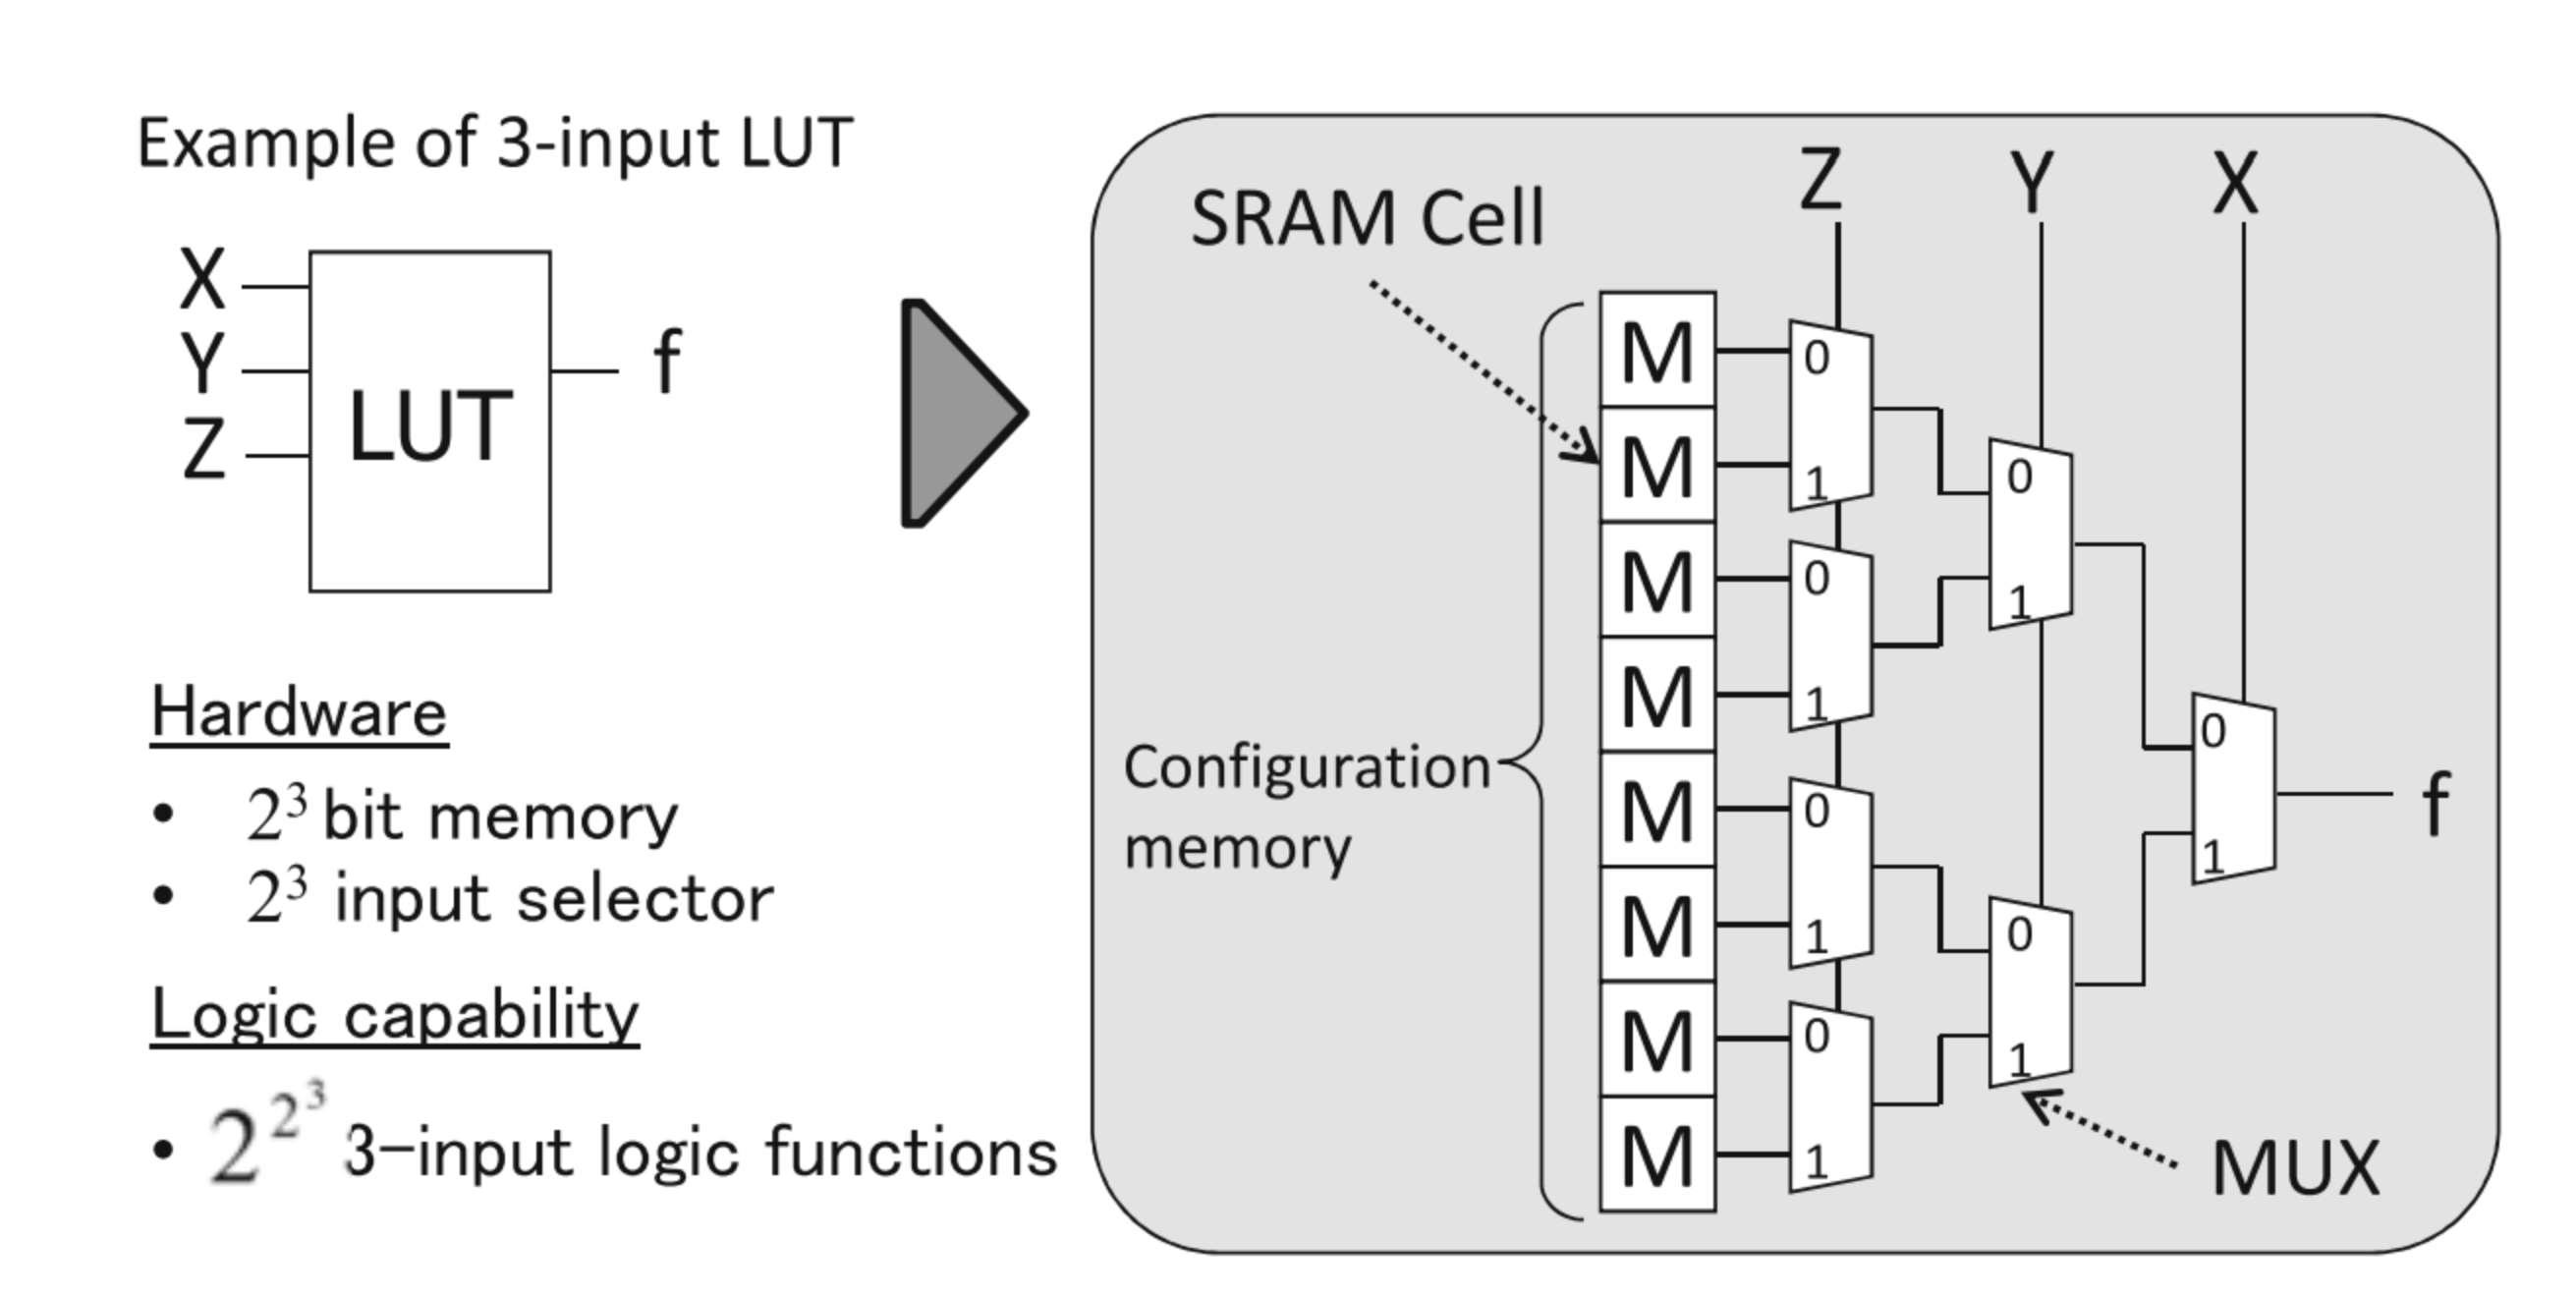
\includegraphics[width=0.75\linewidth]{assets/lut.png}
        \caption{Overview of LUT}
        \label{fig:enter-label}
    \end{figure}
    Ví dụ, một LUT 3 đầu vào (3-input LUT) có \(2^3 = 8\) ô nhớ, mỗi ô lưu trữ một giá trị 0 hoặc 1. Nếu chúng ta muốn lập trình LUT để thực hiện hàm logic \(F(A, B, C) = A \land (B \lor C)\), chúng ta sẽ điền bảng giá trị như sau:
    
    \begin{table}[h]
        \centering
        \begin{tabular}{|c|c|c|c|}
            \hline
            A & B & C & F(A, B, C) \\
            \hline
            0 & 0 & 0 & 0 \\
            0 & 0 & 1 & 0 \\
            0 & 1 & 0 & 0 \\
            0 & 1 & 1 & 0 \\
            1 & 0 & 0 & 0 \\
            1 & 0 & 1 & 1 \\
            1 & 1 & 0 & 1 \\
            1 & 1 & 1 & 1 \\
            \hline
        \end{tabular}
        \caption{Bảng chân trị của F(A, B, C)}
        \label{tab:truth_table}
    \end{table}
    
    Trong trường hợp này, LUT sẽ được lập trình bằng cách lưu trữ các giá trị đầu ra (0, 0, 0, 0, 0, 1, 1, 1) vào 8 ô nhớ. Khi FPGA hoạt động, các đầu vào A, B, và C sẽ được sử dụng để tra cứu (lookup) giá trị đầu ra tương ứng từ bảng. Điều này cho phép LUT thực hiện bất kỳ hàm logic nào với 3 biến đầu vào, từ các hàm đơn giản (như AND, OR) đến các hàm phức tạp hơn.
    \begin{figure}[H]
        \centering
        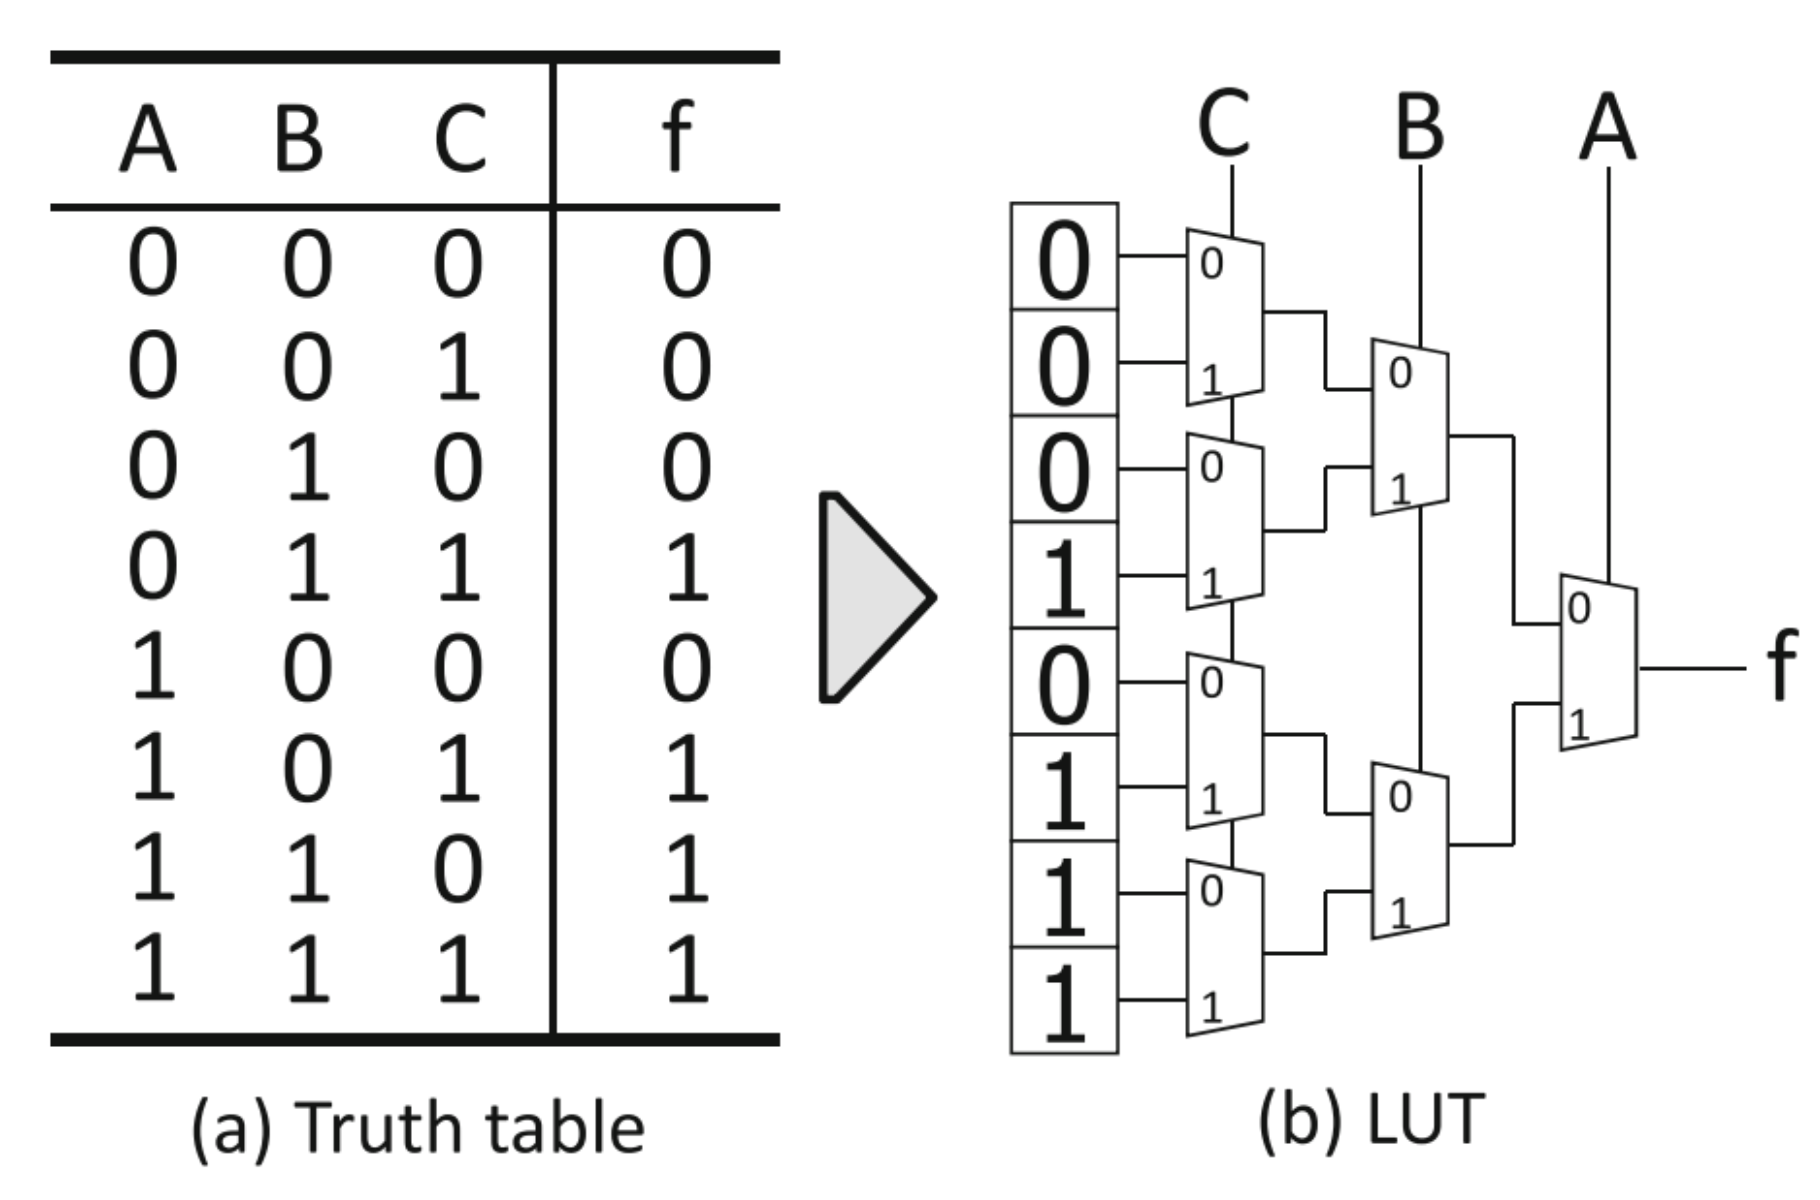
\includegraphics[width=0.5\linewidth]{assets/tt-lut.png}
        \caption{Implementation of majority vote by LUT}
        \label{fig:enter-label}
    \end{figure}
    Trong FPGA hiện đại, LUT thường có 4 đến 6 đầu vào (4-input hoặc 6-input LUT), vì số đầu vào lớn hơn cho phép thực hiện các hàm logic phức tạp hơn mà không cần kết hợp nhiều LUT. Tuy nhiên, số đầu vào lớn cũng làm tăng kích thước bộ nhớ của LUT (ví dụ, một 6-input LUT cần \(2^6 = 64)\) ô nhớ), dẫn đến chi phí về diện tích và năng lượng.
    \item \textbf{Flip-Flops (FFs)} là các phần tử lưu trữ (storage elements) trong FPGA, được sử dụng để lưu trữ trạng thái hoặc đồng bộ hóa tín hiệu. Một flip-flop là một mạch tuần tự (sequential circuit) có khả năng lưu trữ một bit dữ liệu (0 hoặc 1), và giá trị của nó chỉ thay đổi khi nhận được tín hiệu xung nhịp (clock signal). Trong sơ đồ, flip-flop được biểu thị bằng một khối "FF" bên cạnh LUT, với một đầu ra được kết nối với mạng định tuyến.
    
    Flip-flops thường được sử dụng để:
    \begin{itemize}
        \item Lưu trữ trạng thái: Trong các mạch tuần tự, như bộ đếm (counter) hoặc máy trạng thái hữu hạn (finite state machine - FSM), flip-flops lưu trữ trạng thái hiện tại của hệ thống. Ví dụ, một bộ đếm 4-bit cần 4 flip-flops để lưu trữ giá trị hiện tại của bộ đếm.
        \item Đồng bộ hóa tín hiệu: Flip-flops đảm bảo rằng các tín hiệu trong FPGA được đồng bộ với xung nhịp, tránh các vấn đề như \textbf{race condition} (điều kiện cạnh tranh) hoặc \textbf{glitch} (nhiễu tín hiệu). Ví dụ, đầu ra của một LUT có thể được truyền qua một flip-flop để đảm bảo rằng tín hiệu chỉ thay đổi vào các cạnh xung nhịp (clock edge).
    \end{itemize}
    
    Trong một khối logic, LUT và flip-flop thường được kết hợp với nhau để tạo thành một đơn vị cơ bản gọi là \textbf{slice} (trong FPGA của Xilinx) hoặc \textbf{logic element (LE)} (trong FPGA của Intel). Một slice điển hình bao gồm một hoặc nhiều LUT, một hoặc nhiều flip-flop, và một bộ chọn (multiplexer) để quyết định liệu đầu ra của slice sẽ lấy trực tiếp từ LUT (cho các mạch tổ hợp - combinational logic) hay từ flip-flop (cho các mạch tuần tự - sequential logic).
    

\end{itemize}
\subsubsection{Programmable Routing} 
\textbf{Programmable routing} (mạng định tuyến có thể lập trình), được biểu thị bằng các đường zigzag kết nối các khối logic. Mạng định tuyến là một thành phần quan trọng của FPGA, cho phép tín hiệu được truyền giữa các khối logic, cũng như giữa các khối logic và các chân I/O.
\begin{itemize}
    \item Cấu trúc của mạng định tuyến: \par
    Mạng định tuyến bao gồm các \textbf{wires} (đường dây) và các \textbf{switches} (điểm chuyển mạch) có thể lập trình. Các đường dây được tổ chức thành các kênh định tuyến (routing channels) chạy ngang và dọc qua FPGA, tạo thành một lưới kết nối. Các điểm chuyển mạch, thường được triển khai bằng các \textbf{pass transistors} hoặc \textbf{multiplexers}, cho phép người dùng cấu hình cách các đường dây được kết nối với nhau. Ví dụ, một tín hiệu từ đầu ra của một LUT có thể được định tuyến đến đầu vào của một LUT khác, hoặc đến một chân I/O, bằng cách bật/tắt các điểm chuyển mạch phù hợp.
    \item Tính linh hoạt: \par Tính "có thể lập trình" của mạng định tuyến là yếu tố then chốt làm cho FPGA linh hoạt. Người dùng có thể định tuyến tín hiệu theo bất kỳ cách nào cần thiết để thực hiện chức năng mong muốn. Ví dụ, trong một ứng dụng xử lý tín hiệu, tín hiệu đầu vào có thể được định tuyến qua một chuỗi các khối logic để thực hiện FFT (Fast Fourier Transform), sau đó được định tuyến đến một chân I/O để xuất kết quả.
    \item Chi phí overhead: \par
    Mặc dù mạng định tuyến mang lại tính linh hoạt, nó cũng gây ra chi phí overhead về diện tích, độ trễ, và năng lượng. Trong FPGA, mạng định tuyến thường chiếm 70-80\% diện tích chip, vì cần rất nhiều đường dây và điểm chuyển mạch để đảm bảo tính linh hoạt. Ngoài ra, việc truyền tín hiệu qua nhiều điểm chuyển mạch có thể gây ra độ trễ (delay), làm giảm tần số hoạt động (clock frequency) của FPGA so với ASICs.

\end{itemize}

\subsubsection{I/O Pins} 
I/O pins là một thành phần không thể thiếu trong thiết kế FPGA, đóng vai trò là cầu nối giữa FPGA và thế giới bên ngoài. Mỗi I/O pin được hỗ trợ bởi một I/O block, bao gồm bộ đệm đầu vào, bộ đệm đầu ra, điều khiển ba trạng thái, và các tính năng có thể lập trình như drive strength, slew rate, và termination. I/O pins cho phép FPGA nhận dữ liệu đầu vào, gửi dữ liệu đầu ra, và hỗ trợ các giao thức giao tiếp tốc độ cao, với khả năng tương thích với nhiều chuẩn tín hiệu và mức điện áp khác nhau. Mặc dù đối mặt với các thách thức như số lượng giới hạn, nhiễu tín hiệu, và tiêu thụ năng lượng, I/O pins là yếu tố then chốt giúp FPGA trở thành một nền tảng linh hoạt cho nhiều ứng dụng, từ xử lý tín hiệu, viễn thông, đến hệ thống nhúng. Trong bối cảnh Reconfigurable Computing, I/O pins đảm bảo rằng FPGA có thể giao tiếp hiệu quả với các thiết bị bên ngoài, hỗ trợ việc triển khai các mảng không gian và mạng định tuyến có thể cấu hình để đạt được hiệu suất cao và tính linh hoạt.

Số lượng I/O pins trên một FPGA có thể dao động từ vài chục đến hàng nghìn, tùy thuộc vào kích thước và mục đích của chip. Ví dụ, một FPGA nhỏ như Xilinx Spartan-6 có thể có khoảng 100-200 I/O pins, trong khi một FPGA cao cấp như Xilinx Virtex UltraScale+ có thể có hơn 1000 I/O pins. Số lượng I/O pins là một yếu tố quan trọng trong thiết kế hệ thống, vì nó xác định khả năng giao tiếp của FPGA với các thiết bị bên ngoài.
\subsection{Problems \& limitations}
Các thách thức liên quan đến lập trình FPGA, với các điểm chính như sau:
\begin{itemize}
    \item Low-level coding in hardware language (Verilog, VHDL):\par Một trong những vấn đề lớn nhất khi làm việc với FPGA là yêu cầu lập trình bằng các ngôn ngữ phần cứng cấp thấp (Hardware Description Languages - HDLs) như Verilog hoặc VHDL. Không giống như các ngôn ngữ lập trình cấp cao như C hoặc Python, vốn trừu tượng hóa phần cứng và cho phép người dùng tập trung vào logic thuật toán, Verilog và VHDL yêu cầu người dùng mô tả chi tiết các thành phần phần cứng (như cổng logic, flip-flops) và cách chúng được kết nối. Ví dụ, để triển khai một bộ đếm 4-bit trên FPGA, người dùng phải viết mã Verilog để định nghĩa các flip-flops, cổng logic, và kết nối giữa chúng, thay vì chỉ viết một vòng lặp đơn giản như trong C. Điều này làm tăng độ phức tạp và thời gian phát triển, đặc biệt đối với các nhà phát triển phần mềm không quen với thiết kế phần cứng.
    \item Lots of work on “high-level synthesis” from FPGA vendors: \par Để giải quyết vấn đề lập trình cấp thấp, các nhà cung cấp FPGA (như Xilinx và Intel) đã đầu tư mạnh vào High-Level Synthesis (HLS), một công nghệ cho phép người dùng viết mã bằng các ngôn ngữ cấp cao như C, C++, hoặc SystemC, sau đó tự động chuyển đổi mã này thành HDL. Ví dụ, công cụ Vivado HLS của Xilinx cho phép người dùng viết một hàm C để thực hiện nhân ma trận, và công cụ sẽ tự động tạo ra mã Verilog tương ứng để triển khai trên FPGA. Tuy nhiên, hình ảnh lưu ý rằng HLS vẫn "Traditionally, awful to use" (Theo truyền thống, rất khó sử dụng), vì các công cụ HLS ban đầu thường tạo ra mã không tối ưu, dẫn đến hiệu suất thấp hoặc sử dụng tài nguyên không hiệu quả. Dù vậy, hình ảnh cũng ghi nhận rằng HLS "might be close to an inflection point" (có thể đang tiến gần đến một bước ngoặt), ám chỉ rằng các cải tiến gần đây (tính đến năm 2019) đã làm cho HLS trở nên khả thi hơn, với các công cụ như Vivado HLS và Intel HLS Compiler cung cấp hiệu suất tốt hơn và dễ sử dụng hơn.
    \item Synthesis (compilation) can take many hours! Common workflow: start compilation, go home, test next morning, repeat:\par
    Một vấn đề lớn khác trong lập trình FPGA là thời gian biên dịch (synthesis) kéo dài, có thể mất nhiều giờ, đặc biệt đối với các thiết kế phức tạp. Quá trình biên dịch FPGA bao gồm nhiều bước: tổng hợp (synthesis), ánh xạ (mapping), đặt (placement), và định tuyến (routing). Ví dụ, trong bước tổng hợp, mã Verilog được chuyển thành một netlist (danh sách mạng) gồm các cổng logic; trong bước ánh xạ, netlist được ánh xạ lên các LUT (Lookup Tables); và trong bước đặt và định tuyến, các LUT được đặt vào vị trí vật lý trên chip và kết nối với nhau qua mạng định tuyến. Mỗi bước này là một bài toán tính toán phức tạp (thường là NP-hard), đòi hỏi các thuật toán heuristic tốn nhiều thời gian. Hình ảnh mô tả một quy trình làm việc phổ biến: người dùng bắt đầu biên dịch, về nhà, kiểm tra kết quả vào sáng hôm sau, và lặp lại nếu có lỗi. Điều này làm chậm quá trình phát triển và gỡ lỗi (debugging), đặc biệt khi so sánh với phần mềm, nơi biên dịch chỉ mất vài giây hoặc phút.

\end{itemize}
\subsection{FPGA trong bộ tăng tốc học sâu (DL Acceleration)}
\subsubsection{Yêu cầu chính của Tăng tốc DL }
\begin{figure} [!h]
    \centering
    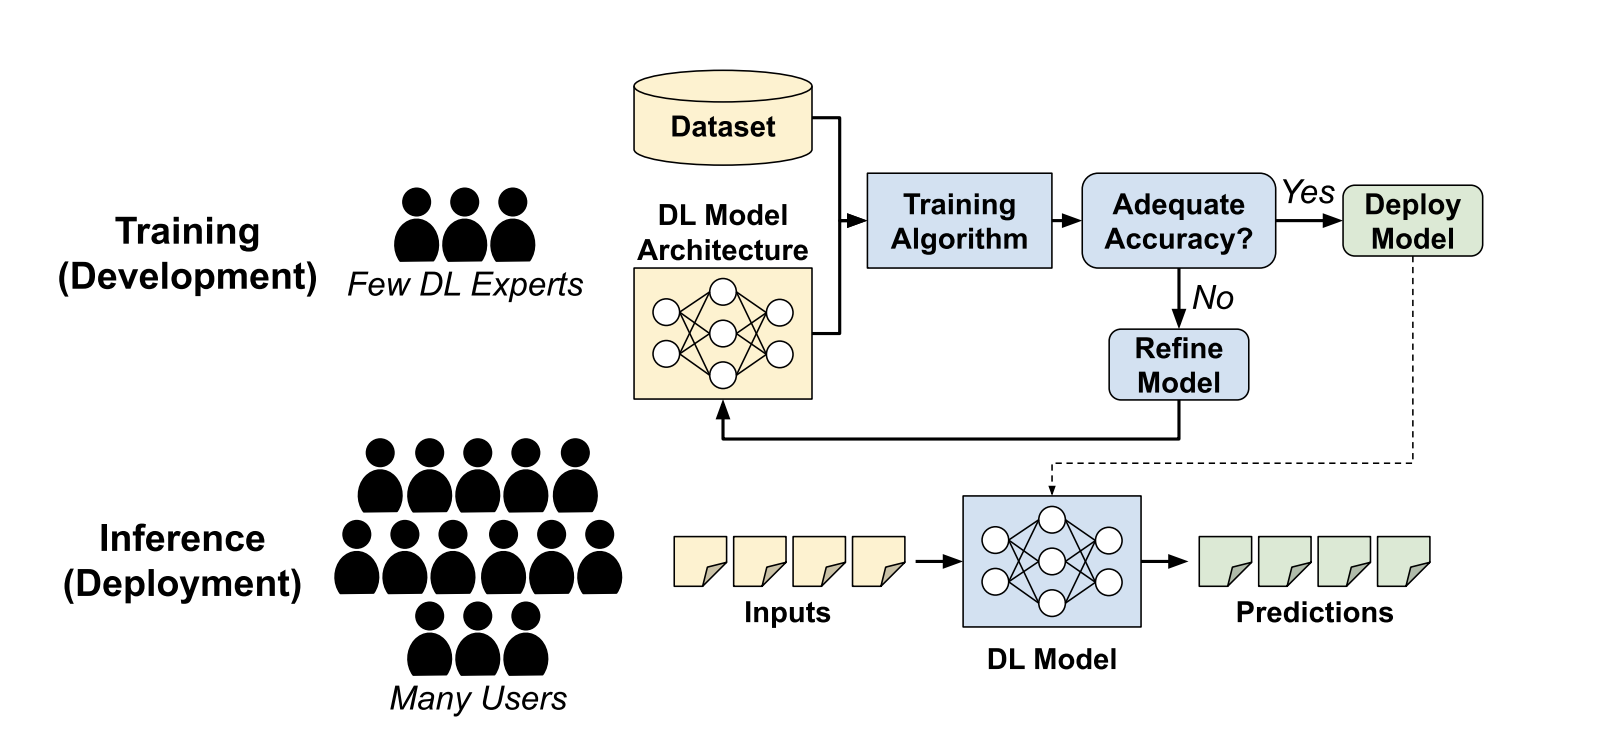
\includegraphics[width=0.75\linewidth]{assets/fpga_2.png}
    \caption{Các giai đoạn huấn luyện và suy luận của một mô hình học sâu (DL): Giai đoạn huấn luyện được thực hiện bởi một vài chuyên gia DL trên các cụm máy tính quy mô lớn và yêu cầu nhiều vòng lặp thiết kế. Khi độ chính xác của mô hình đạt yêu cầu, mô hình sẽ được triển khai để suy luận với các yêu cầu hiệu năng khác nhau tùy theo ứng dụng (chịu trễ được so với thời gian thực).}
    \label{fig:fpga_2}
\end{figure}

Như được minh họa trong hình \ref{fig:fpga_2}, một mô hình học sâu (DL) trải qua hai giai đoạn chính trong vòng đời: huấn luyện và suy luận.

Trong quá trình huấn luyện, một nhóm nhỏ các nhà nghiên cứu DL sẽ thiết kế kiến trúc mô hình và huấn luyện nó bằng cách sử dụng các tập dữ liệu khổng lồ (ví dụ: trên 570 GB đối với mô hình ngôn ngữ GPT-3) nhằm đạt được chất lượng kết quả mong muốn. Quá trình này đòi hỏi tài nguyên tính toán và bộ nhớ rất lớn do khối lượng dữ liệu khổng lồ, và thường phải trải qua hàng chục đến hàng trăm vòng lặp thiết kế để tối ưu hóa mô hình. Do đó, quá trình huấn luyện thường được thực hiện trên các cụm máy tính và bộ tăng tốc quy mô lớn trong các trung tâm dữ liệu. Sản phẩm cuối cùng của quá trình huấn luyện là kiến trúc mô hình cùng với các giá trị của các tham số (trọng số) có thể huấn luyện, sau đó được triển khai trong các ứng dụng quy mô sản xuất để thực hiện suy luận trên các mẫu dữ liệu mới chưa có trong tập huấn luyện ban đầu.

Tùy thuộc vào môi trường triển khai (đám mây/trung tâm dữ liệu so với thiết bị biên/nhúng) và tính chất của ứng dụng (cho phép một mức độ độ trễ nhất định so với ứng dụng thời gian thực), quá trình suy luận DL có thể có các yêu cầu tính toán và hạn chế riêng. Do đó, phần cứng sử dụng để tăng tốc huấn luyện và suy luận DL cần được tối ưu hóa theo các chỉ số và trường hợp sử dụng khác nhau, tạo ra thị trường tiềm năng cho các nền tảng tăng tốc khác nhau (ví dụ: GPU, FPGA, ASIC) dựa trên những ưu và nhược điểm đặc trưng của chúng.

\textbf{1) Hiệu suất:}

\begin{itemize}
    \item \textbf{Thông lượng (Throughput):} Là số lượng mẫu đầu vào mà một bộ tăng tốc cụ thể có thể xử lý trong một đơn vị thời gian trên một tải công việc DL nhất định. Để thuận tiện so sánh hiệu quả của các bộ tăng tốc giữa các mô hình có độ phức tạp tính toán khác nhau, thông lượng thường được báo cáo theo đơn vị GOPS hoặc TOPS (tỷ hoặc nghìn tỷ phép toán trên giây), trong đó các phép toán thường được tính bằng tổng số phép nhân và phép tích lũy, vì phép nhân-tích lũy (MAC) là phép toán chủ đạo trong các tải công việc DL. Mỗi bộ tăng tốc có một thông lượng đỉnh (peak throughput) không phụ thuộc vào tải công việc, được xác định bởi số lượng đơn vị MAC thực hiện được trên mỗi chu kỳ nhân với tần số hoạt động tối đa. Tuy nhiên, trên thực tế, không thể đạt được mức sử dụng 100\% của các đơn vị MAC, vì vậy thông lượng hiệu quả (effective throughput) mới là chỉ số thực tế và thường được đánh giá cho từng tải công việc DL. Một kiến trúc bộ tăng tốc hiệu quả sẽ nhằm tối đa hóa mức sử dụng tính toán (tức là thu hẹp khoảng cách giữa thông lượng đỉnh và thông lượng hiệu quả). Để cải thiện thông lượng hiệu quả, nhiều bộ tăng tốc xử lý một lô các đầu vào cùng một lúc. Điều này cho phép tái sử dụng cùng một bộ trọng số mô hình cho nhiều đầu vào trong một lô, từ đó che giấu độ trễ bộ nhớ khi tải bộ trọng số tiếp theo và giảm số chu kỳ mà các đơn vị MAC bị đứng yên. Ngược lại, \textbf{độ trễ} là khoảng thời gian cần thiết để bộ tăng tốc xử lý một mẫu đầu vào duy nhất – đây là chỉ số then chốt đối với các ứng dụng thời gian thực. Mặc dù xử lý theo lô có thể giúp cải thiện thông lượng hiệu quả, nhưng thường làm tăng độ trễ do cần thêm thời gian để tập hợp lô, xử lý toàn bộ lô và xuất kết quả cùng lúc. Ví dụ, đối với mô hình phân loại ảnh ResNet-50, tăng kích thước lô từ 1 lên 8 mẫu giúp cải thiện thông lượng gấp 3 lần nhưng làm tăng độ trễ lên gấp 2.2 lần trên GPU Nvidia V100. Trong giai đoạn huấn luyện, độ trễ không phải là mối quan tâm hàng đầu, do đó các bộ tăng tốc huấn luyện DL được tối ưu hóa theo thông lượng để tối đa hóa số mẫu huấn luyện xử lý trên mỗi giây. Còn đối với suy luận, mục tiêu tối ưu phụ thuộc vào từng trường hợp sử dụng cụ thể; ví dụ, các ứng dụng như công cụ tìm kiếm ảnh dựa trên DL hay kiểm tra bản quyền video chú trọng tối đa số truy vấn người dùng được phục vụ mỗi giây với yêu cầu độ trễ không quá nghiêm ngặt (theo đó ưu tiên thông lượng), trong khi các ứng dụng như phát hiện người đi bộ hay chướng ngại vật trong xe tự lái đòi hỏi độ trễ thấp để đảm bảo an toàn.
\end{itemize}

\textbf{2) Hiệu quả Chi phí và Năng lượng:}

\begin{itemize}
    \item Đối với cả giai đoạn huấn luyện và suy luận, hiệu quả về chi phí và năng lượng là mục tiêu tối ưu hàng đầu cho mọi bộ tăng tốc DL. Ước tính rằng khoảng 35\% tổng chi phí sở hữu của một trung tâm dữ liệu được chi cho điện năng. Khi DL trở thành một tải công việc chủ đạo trong các trung tâm dữ liệu, việc sử dụng phần cứng DL tiết kiệm năng lượng sẽ giúp các nhà cung cấp dịch vụ tiết kiệm chi phí đáng kể. Ví dụ, Google báo cáo rằng việc sử dụng TPU ASIC của họ đã giảm chi phí huấn luyện mô hình ResNet-50 cho bài toán phân loại ảnh đi 38\%. Đối với các mô hình xử lý ngôn ngữ tự nhiên hiện đại như BERT, chi phí này có thể lên đến hàng triệu đô la cho mỗi lần huấn luyện đầy đủ. Bên cạnh đó, việc giảm tiêu thụ điện năng của các trung tâm dữ liệu cũng có tác động lớn đến môi trường, khi mà theo một số ước tính, các trung tâm dữ liệu sẽ tiêu thụ khoảng 8\% tổng điện năng của thế giới vào năm 2030. Ở đầu phổ triển khai, suy luận DL trên các thiết bị biên (edge) chạy bằng pin thường có ngân sách năng lượng rất hạn chế, do đó đòi hỏi phần cứng tính toán phải có hiệu quả năng lượng cao (ví dụ, chip suy luận DL của Tesla được thiết kế riêng với mức tiêu thụ dưới 40W). Mặc dù các ASIC tùy chỉnh có thể mang lại hiệu quả năng lượng vượt trội, nhưng chúng thiếu tính linh hoạt để thích ứng với các hệ thống và thuật toán đa dạng, đồng thời chi phí NRE (non-recurring engineering) và thời gian thiết kế, sản xuất, kiểm thử dài có thể là rào cản đối với các thị trường quy mô nhỏ và vừa.
\end{itemize}

\textbf{3) Tính Thích ứng:}

\begin{itemize}
    \item Bên cạnh việc đạt được hiệu suất cao và tiết kiệm năng lượng, các bộ tăng tốc DL cũng phải có tính linh hoạt để thích ứng với những thay đổi thường xuyên của thuật toán. Các mô hình DL mới được giới thiệu với tốc độ nhanh hơn nhiều so với chu kỳ thiết kế và triển khai của phần cứng truyền thống. Tính thích ứng có thể đạt được thông qua việc làm cho một hoặc nhiều thành phần của hệ thống có thể lập trình được bằng phần mềm; tuy nhiên, khả năng lập trình bằng phần mềm thường mang lại thêm chi phí về năng lượng và hiệu suất (ví dụ, chi phí lấy lệnh và giải mã lệnh) so với phần cứng cố định. Hơn nữa, bộ tăng tốc DL, đặc biệt là trong các triển khai tại biên, thường là một phần của hệ thống lớn hơn – nơi nó cần giao tiếp với nhiều loại cảm biến (ví dụ: camera, LiDAR) và bộ điều khiển (ví dụ: hệ thống phanh) với các giao thức truyền thông, yêu cầu tiền xử lý và hậu xử lý dữ liệu khác nhau. Do đó, tính thích ứng không chỉ là yêu cầu của phần cứng tính toán DL mà còn của khả năng giao tiếp với các thành phần khác trong hệ thống, nhằm đảm bảo khả năng sử dụng rộng rãi trong nhiều trường hợp triển khai. Việc cho phép giao tiếp linh hoạt này thường đòi hỏi khả năng thích ứng về điện (ví dụ: yêu cầu về điện áp và thời gian khác nhau của các giao thức) – điều mà lập trình phần mềm không thể đảm bảo một cách độc lập.
\end{itemize}


\subsubsection{Ưu điểm của FPGA trong Tăng tốc DL}
\begin{figure} [!h]
    \centering
    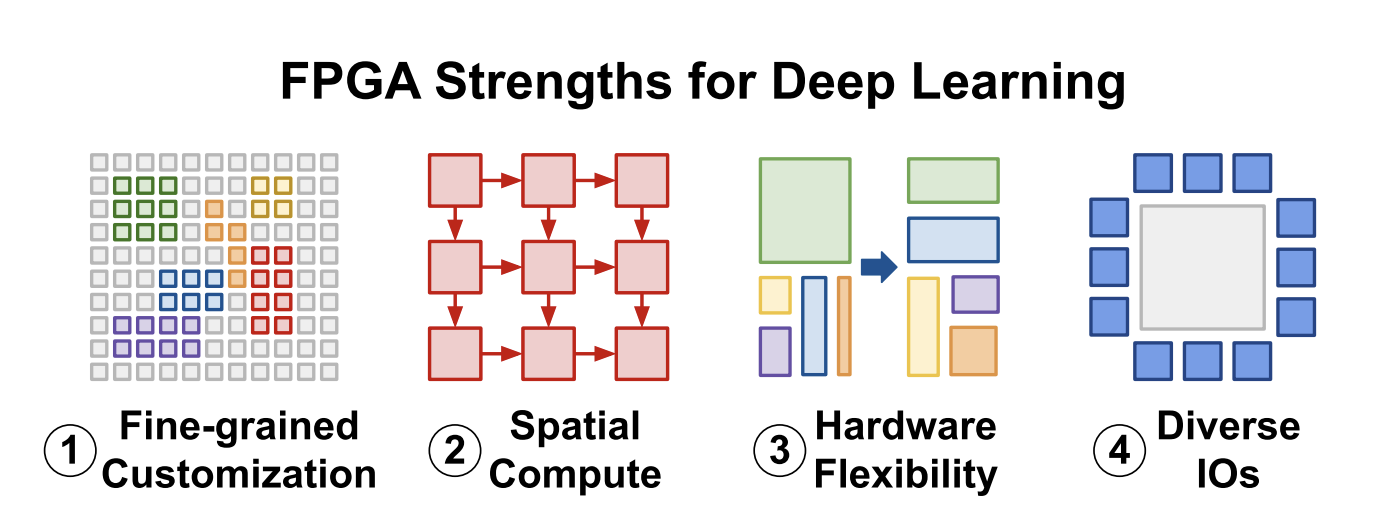
\includegraphics[width=0.75\linewidth]{assets/fpga_3.png}
    \caption{Các đặc điểm nổi bật của FPGA khiến chúng trở thành nền tảng tăng tốc hiệu quả cho học sâu (DL)}
    \label{fig:fpga_3}
\end{figure}
Dựa trên các yêu cầu tăng tốc DL được trình bày ở mục trên, ta có thể nhận diện một số ưu điểm chính của FPGA (được tóm tắt trong hình \ref{fig:fpga_3}) khiến chúng trở thành nền tảng tăng tốc hấp dẫn và hiệu quả cho các trường hợp sử dụng DL cụ thể.

\textbf{Thứ nhất,} FPGA cung cấp khả năng lập trình phần cứng ở mức chi tiết, cho phép xây dựng các đường truyền dữ liệu tính toán và các hệ thống bộ nhớ on-chip được tùy chỉnh chính xác theo nhu cầu của ứng dụng. Do đó, FPGA có ưu thế so với các bộ xử lý đa năng (như CPU và GPU) trong các trường hợp đòi hỏi sự tùy chỉnh cao. Ví dụ, chất lượng kết quả suy luận DL có thể chấp nhận được ngay cả với tính toán độ chính xác thấp, và vì năng lượng cũng như diện tích của các đơn vị tính toán giảm nhanh theo độ chính xác, điều này được khai thác để tạo ra giải pháp tăng tốc hiệu quả hơn. Không giống như CPU và GPU chỉ hỗ trợ một số độ chính xác số học nhất định (ví dụ: int4, int8, fp16, fp32), FPGA có thể triển khai các đơn vị tính toán tùy chỉnh cho bất kỳ độ chính xác nào, bao gồm cả nhị phân/ba trạng, các định dạng số thực hẹp (ví dụ: fp8), hoặc các số thực có số mũ chia sẻ (bfp). Vì độ chính xác tối ưu có thể khác nhau giữa các mô hình DL và thậm chí giữa các lớp trong cùng một mô hình, sự linh hoạt này trở nên vô cùng hữu ích. Tuy nhiên, khả năng lập trình phần cứng ở mức chi tiết đi kèm với một số chi phí về tốc độ và diện tích, do các chức năng được triển khai qua các khối lập trình được và mạch định tuyến lập trình được vốn chậm hơn và chiếm diện tích lớn hơn so với các cổng logic của cell tiêu chuẩn và dây dẫn trực tiếp. Vì vậy, lợi ích từ việc tùy chỉnh phải vượt trội so với những chi phí phụ trội này để giải pháp tăng tốc FPGA có tính cạnh tranh.

\textbf{Thứ hai,} FPGA là thiết bị tính toán không gian. Điều này có nghĩa là dữ liệu không cần phải di chuyển qua hệ thống bộ nhớ phân cấp gồm các bộ nhớ cache và các file register để thực hiện phép tính, và các lõi tính toán cũng không cần giao tiếp qua bộ nhớ. Thay vào đó, trên FPGA, dữ liệu có thể được chuyển trực tiếp từ các bộ đệm on-chip phân tán và qua các đơn vị tính toán nối tiếp nhờ vào mạch định tuyến lập trình linh hoạt, mà không cần một chuỗi lệnh điều phối chuyển động dữ liệu và các phép tính. Phương pháp này giúp giảm tổng độ trễ tính toán vì ít chu kỳ bị tiêu tốn cho việc di chuyển dữ liệu qua các tầng bộ nhớ, đồng thời mang lại tiết kiệm năng lượng đáng kể; ví dụ, khoảng 99\% năng lượng tiêu thụ cho một phép cộng số nguyên trên CPU 45nm được sử dụng cho việc truy cập cache/register file và logic điều khiển – phần lớn năng lượng này có thể được tiết kiệm khi thực hiện các phép tính trực tiếp trên FPGA theo kiểu không gian.

\textbf{Thứ ba,} FPGA có tính linh hoạt cao. Việc cấu hình lại FPGA bằng một bitstream mới sẽ thay đổi hoàn toàn chức năng phần cứng của nó. Điều này mang lại lợi thế rõ ràng so với các bộ tăng tốc ASIC vì phần cứng có thể linh hoạt thích ứng với các thay đổi nhanh chóng trong thuật toán DL, kiến trúc mô hình và các yêu cầu tiền xử lý hoặc hậu xử lý đặc thù của ứng dụng. Các phép toán mới có thể được triển khai trực tiếp trên phần cứng, tích hợp vào kiến trúc tăng tốc dựa trên FPGA và được triển khai trong môi trường sản xuất chỉ trong vài tuần. Ngược lại, một bộ tăng tốc ASIC sẽ phải triển khai phép toán mới đó trên lõi lập trình được bằng phần mềm hoặc trên CPU chủ, dẫn đến hiệu năng giảm cho đến khi chip thế hệ mới được thiết kế, sản xuất và triển khai – quá trình có thể kéo dài hàng năm.

\textbf{Thứ tư,} FPGA cung cấp vô số giao diện vào/ra (I/O) có thể lập trình được. Những giao diện này có thể được cấu hình linh hoạt để hỗ trợ nhiều giao thức khác nhau với các đặc tính điện và yêu cầu thời gian đa dạng. Các FPGA hiện đại cũng tích hợp sẵn các bộ điều khiển cứng cho các tiêu chuẩn được sử dụng rộng rãi trong các trung tâm dữ liệu như Ethernet, PCIe (Peripheral Component Interconnect Express) và các bộ nhớ ngoài DDR (Double Data Rate) hoặc HBM (High Bandwidth Memory). Điều này cho phép giao tiếp hiệu quả giữa FPGA dưới dạng thẻ tăng tốc máy chủ và CPU chủ, đồng thời cũng cho phép kết nối trực tiếp nhiều FPGA qua mạng để tạo thành các hệ thống tăng tốc với nhiều thiết bị, ví dụ như bộ tăng tốc DL quy mô trung tâm dữ liệu của Microsoft – Brainwave. Thêm vào đó, logic lập trình được của FPGA còn có thể triển khai các tiêu chuẩn tùy chỉnh khác để giao tiếp với các cảm biến hoặc bộ điều khiển trong các hệ thống nhúng tại biên.

Những đặc điểm độc đáo trên dẫn đến một số trường hợp sử dụng DL mà FPGA có lợi thế vượt trội so với các giải pháp tăng tốc khác như CPU/GPU đa năng và ASIC. Cụ thể, FPGA phù hợp với các trường hợp:
\begin{itemize}
    \item \textbf{Thực hiện các phép tính với độ chính xác thấp hoặc định dạng số không tiêu chuẩn:} Các trường hợp này yêu cầu các đường dẫn dữ liệu được tùy chỉnh. Những định dạng độ chính xác này phổ biến và thường dễ sử dụng cho suy luận, trong khi quá trình huấn luyện thường yêu cầu độ chính xác cao (như fp32, fp16) mà các CPU và GPU đa năng hỗ trợ ngay từ đầu.
    \item \textbf{Yêu cầu độ trễ nghiêm ngặt:} Những ứng dụng không cho phép xử lý theo lô với số lượng lớn đầu vào do yêu cầu độ trễ rất thấp. Trong khi các ứng dụng ưu tiên thông lượng có thể xử lý đồng thời nhiều đầu vào, các ứng dụng đòi hỏi độ trễ thấp lại được hưởng lợi từ khả năng xử lý trực tiếp của FPGA, giúp giữ cho các đơn vị tính toán hoạt động liên tục.
    \item \textbf{Có thể chứa toàn bộ trọng số mô hình trong bộ nhớ on-chip:} Tính chất không gian của FPGA cho phép thực hiện tính toán gần bộ nhớ với độ trễ thấp và tổ chức bộ nhớ phù hợp với từng ứng dụng. Đối với các mô hình lớn hơn, các giao diện I/O đa dạng của FPGA cho phép kết nối trực tiếp nhiều FPGA qua mạng để tạo thành hệ thống đa FPGA với nhiều bộ nhớ on-chip.
    \item \textbf{Triển khai thành phần DL trong hệ thống lớn:} Trong các hệ thống như xe tự lái, nơi có nhiều đầu vào từ cảm biến hoặc camera cần được tiền xử lý trước khi đưa vào mô hình DL, và đầu ra của mô hình DL được sử dụng để điều khiển các bộ phận khác nhau, tính linh hoạt và khả năng giao tiếp phong phú của FPGA đóng vai trò quan trọng trong việc tăng tốc toàn bộ hệ thống với các giao diện tùy chỉnh và các quá trình tiền/hậu xử lý phụ thuộc ứng dụng.
    \item \textbf{Yêu cầu thay đổi kiến trúc mô hình DL định kỳ:} Các mô hình DL có thể thay đổi kiến trúc, bổ sung các phép toán mới hoặc có các đồ thị tính toán không đều. Không giống như ASIC, những thay đổi này có thể được triển khai trên phần cứng chỉ bằng cách lập trình lại FPGA với một bitstream mới. Tuy nhiên, nếu những thay đổi diễn ra quá thường xuyên (ví dụ: hàng ngày), việc biên dịch bitstream mới mỗi lần thay đổi mô hình có thể gặp khó khăn do thời gian chạy của các công cụ CAD cho FPGA. Trong những trường hợp như vậy, giải pháp lập trình được bằng phần mềm có thể là lựa chọn khả thi hơn.
\end{itemize}
\subsubsection{Kiểu Tăng tốc Suy luận DL Dựa trên FPGA}
    Trong phần này, chúng ta trình bày các kiểu kiến trúc thường được sử dụng để tăng tốc suy luận DL trên FPGA. Phần này không nhằm mục đích khảo sát toàn diện các bộ tăng tốc suy luận DL được triển khai trên FPGA, vì trọng tâm của chúng ta chủ yếu là các cải tiến đối với kiến trúc chip FPGA.
    
    Năm 2012, AlexNet là mạng nơ-ron tích chập (CNN) đầu tiên chứng minh được chất lượng vượt trội của DL trong các tác vụ phân loại ảnh so với các phương pháp học máy truyền thống. Độ phức tạp tính toán cao của nó đã kích thích sự quan tâm đến việc tăng tốc suy luận DL bằng phần cứng chuyên dụng trên FPGA với vai trò là bộ xử lý phụ. Một CPU chủ hoặc CPU nhúng sẽ chuyển toàn bộ tính toán của CNN (hoặc các lớp tính toán nặng cụ thể) sang bộ tăng tốc FPGA, và cuối cùng thực hiện một phép toán softmax cuối cùng để tính toán xác suất dự đoán từ đầu ra của bộ tăng tốc, nếu cần. Trong trường hợp này, bộ tăng tốc FPGA thường được thiết kế thủ công và tối ưu hóa cho một mô hình DL cụ thể hoặc một nhóm các mô hình tương tự. Phương pháp này đã đạt được những cải thiện đáng kể về hiệu suất và hiệu quả năng lượng so với các giải pháp phần mềm chạy trên các CPU đa lõi và GPU cùng thời. Tuy nhiên, với sự phát triển liên tục và nhanh chóng của các mô hình DL tiên tiến, nhanh chóng trở nên rõ ràng rằng việc xây dựng một bộ tăng tốc FPGA tùy chỉnh cho từng mô hình là vô cùng tốn công sức và không thể theo kịp sự tiến hóa của mô hình DL.
    
    Do đó, xây dựng các bộ sinh phần cứng tùy chỉnh để tự động hóa quá trình này đã trở thành trọng tâm nghiên cứu quan trọng. Các bộ sinh phần cứng này là các trình biên dịch chuyên ngành nhận đầu vào là các đặc tả của FPGA mục tiêu và đồ thị luồng dữ liệu của một mô hình DL theo định dạng được sử dụng phổ biến trong các khung DL như TensorFlow hoặc PyTorch. Chúng tối ưu hóa đồ thị luồng dữ liệu bằng cách sắp xếp lại, đơn giản hóa và/hoặc gộp các lớp/phép toán của mô hình, sau đó sử dụng thư viện các mô-đun phần cứng có tham số để tạo ra một triển khai FPGA được tối ưu hóa cho mô hình dựa trên các giới hạn tài nguyên của FPGA mục tiêu. Mặc dù các quy trình sinh phần cứng DL này đều chia sẻ những khái niệm cơ bản giống nhau, nhưng kiến trúc bộ tăng tốc được tạo ra có thể rất khác nhau. Một số quy trình sinh tạo ra kiến trúc dựa trên dòng dữ liệu xếp lớp (pipeline) trong đó mỗi lớp có một đơn vị tính toán riêng và tất cả các lớp được thực thi trên FPGA theo dạng pipeline (thực thi không gian). Ví dụ về các quy trình như vậy bao gồm HPIPE, fpgaConvNet, DNNBuilder và FINN. Các quy trình khác tạo ra kiến trúc có các phần tử xử lý (PEs) linh hoạt hơn, trên đó các lớp của một mô hình được ánh xạ và thực thi tuần tự (thực thi theo thời gian) dưới sự điều phối của các máy trạng thái hữu hạn và microcode. Nhiều quy trình tự động áp dụng các tối ưu hóa thân thiện với DL trên FPGA nhằm tăng cường hiệu suất, chẳng hạn như lượng tử hóa xuống độ chính xác số học thấp hơn và khai thác tính hiếm (sparsity) để bỏ qua các phép tính không hiệu quả với trọng số bằng 0.

    \begin{figure} [!h]
        \centering
        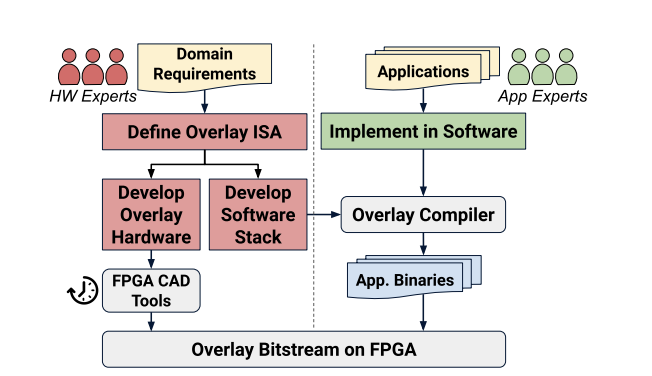
\includegraphics[width=0.75\linewidth]{assets/fpga_4.png}
        \caption{Cách tiếp cận thiết kế overlay cho phép các chuyên gia ứng dụng sử dụng FPGA để tăng tốc các khối lượng công việc học sâu (DL) mà không cần có chuyên môn về thiết kế phần cứng hoặc phải chịu thời gian chạy lâu của các công cụ thiết kế FPGA (CAD tools).}
        \label{fig:fpga_4}
    \end{figure}
    
    \textbf{Lưu ý:} Hình \ref{fig:fpga_4} minh họa cách tiếp cận thiết kế overlay, cho phép các chuyên gia ứng dụng sử dụng FPGA để tăng tốc tải công việc DL mà không cần có chuyên môn thiết kế phần cứng, đồng thời không phải chịu thời gian chạy lâu của các công cụ CAD cho FPGA.
    
    Một số công trình thậm chí còn đi xa hơn, trực tiếp sử dụng các bảng tra cứu (LUTs) trong FPGA làm các khối xây dựng có thể huấn luyện của một mạng nơ-ron thay vì chỉ sử dụng các phép toán MAC.
    
    Việc tạo ra phần cứng DL tùy chỉnh khai thác được đặc tính tái cấu hình độc đáo của FPGA bằng cách tối ưu hóa kiến trúc bộ tăng tốc sao cho phù hợp hoàn toàn với nhu cầu của một mô hình hoặc một nhóm mô hình cụ thể, qua đó giảm thiểu các chi phí phụ trội của tính tổng quát. Tuy nhiên, điều này đi kèm với (1) thời gian biên dịch FPGA kéo dài (trong khoảng vài giờ cho quá trình tổng hợp, định vị và định tuyến) để tạo ra một bitstream FPGA khác nhau cho mỗi mô hình mới hoặc thay đổi nhẹ trong mô hình hiện có và (2) việc cần phải lập trình lại FPGA (có thể mất vài chục đến vài trăm mili giây) khi chuyển đổi giữa các bitstream được biên dịch sẵn cho các mô hình khác nhau. Những nhược điểm này có thể gây cản trở đối với các trường hợp cần cập nhật mô hình rất thường xuyên (ví dụ: hàng ngày) trong môi trường sản xuất hoặc khi cần chuyển đổi theo thời gian thực hoặc theo đầu vào giữa nhiều mô hình.
    
    Một hướng tiếp cận khác trong thiết kế bộ tăng tốc DL trên FPGA là xây dựng các overlay chuyên ngành có thể lập trình được bằng phần mềm. Tương tự như CPU và GPU, một overlay FPGA định nghĩa một kiến trúc tập lệnh (ISA) nhằm tách rời phần cứng và phần mềm. ISA này ẩn đi tất cả các chi tiết về vi kiến trúc và cài đặt phần cứng khỏi các nhà phát triển ứng dụng, những người viết thuật toán của mình bằng ngôn ngữ lập trình cấp cao và sau đó biên dịch chúng thành các chuỗi lệnh có thể chạy trên bất kỳ bộ xử lý nào hỗ trợ cùng một ISA. Đối với một kiến trúc và ISA chung (ví dụ: RISC-V), một triển khai ASIC cứng sẽ luôn hiệu quả hơn so với overlay FPGA do chi phí thêm của tính tái cấu hình. Tuy nhiên, một bộ xử lý mềm có thể tăng cường hiệu suất bằng cách khai thác tính linh hoạt của FPGA để triển khai một đường truyền dữ liệu và hệ thống bộ nhớ được tùy chỉnh, cũng như một ISA chuyên ngành.
    
    Như được minh họa trong hình \ref{fig:fpga_4}, để xây dựng một overlay DL trên FPGA, các kiến trúc sư sẽ đầu tiên thiết kế ISA overlay và kiến trúc bộ xử lý. Sau đó, vi kiến trúc của overlay được tối ưu hóa mạnh mẽ để tạo ra một triển khai FPGA chất lượng cao duy nhất, được triển khai trên FPGA và được lập trình qua phần mềm để thực thi các mô hình DL khác nhau. Để lập trình overlay, người dùng được cung cấp một trình biên dịch chuyển đổi mô tả cấp cao của một mô hình DL (ví dụ: TensorFlow hoặc PyTorch) thành một chuỗi lệnh để thực thi trên overlay FPGA. Trong cách tiếp cận này, người dùng không cần có bất kỳ kiến thức thiết kế phần cứng nào, từ đó giảm đáng kể rào cản cho các nhà phát triển ứng dụng DL khi sử dụng FPGA. Thêm vào đó, thời gian lặp lại để biên dịch một mô hình DL mới nhanh hơn nhiều, vì chỉ cần thực hiện biên dịch phần mềm (trong vài giây) thay vì biên dịch phần cứng FPGA (trong vài giờ) để tạo ra một bitstream mới. Có rất nhiều ví dụ về overlay DL từ cả ngành công nghiệp và học thuật được tối ưu hóa cho các loại mô hình khác nhau, bao gồm cả bộ tăng tốc suy luận DL quy mô trung tâm dữ liệu của Microsoft – Brainwave.
\subsubsection{Ví dụ về Tăng tốc DL trên FPGA}
    Khi sử dụng FPGA cho tăng tốc suy luận DL, bất kể kiểu thiết kế của bộ tăng tốc, có hai mối quan tâm chính. Mối quan tâm đầu tiên là tính dễ sử dụng; FPGA thường khó thiết kế, sử dụng và gỡ lỗi hơn so với các nền tảng tính toán khác như GPU và CPU. Ngay cả khi có những tiến bộ trong công nghệ tổng hợp cấp cao (HLS), việc sử dụng FPGA vẫn đòi hỏi kiến thức chuyên sâu về thiết kế phần cứng, khiến chúng khó tiếp cận đối với các nhà phát triển ứng dụng DL. Mối quan tâm thứ hai là liệu FPGA có thể cung cấp hiệu suất suy luận DL đạt chuẩn hàng đầu hay không, mặc dù chúng có những chi phí phụ thuộc vốn có của tính tái cấu hình. Như đã thảo luận ở phần trước, cả hai cách tiếp cận tạo phần cứng tùy chỉnh và thiết kế overlay đều giải quyết mối quan tâm đầu tiên, cho phép các nhà phát triển ứng dụng DL chuyển từ mô tả mô hình DL cấp cao sang triển khai trên FPGA mà không cần nhiều kiến thức thiết kế phần cứng.

Trong phần này, chúng ta trình bày hai ví dụ điển hình từ hai cách tiếp cận thiết kế này để cho thấy rằng FPGA có thể đạt được hiệu suất suy luận DL xuất sắc. Chúng ta cũng chỉ ra rằng hiệu suất cao hơn nữa có thể đạt được bằng cách tối ưu hóa kiến trúc FPGA bên dưới dành riêng cho DL.

\textbf{1) Ví dụ Tạo phần cứng tùy chỉnh (HPIPE - Heterogeneous Layer-Pipelined and Sparse-Aware CNN Inference for FPGAs):}

\begin{figure} [!h]
    \centering
    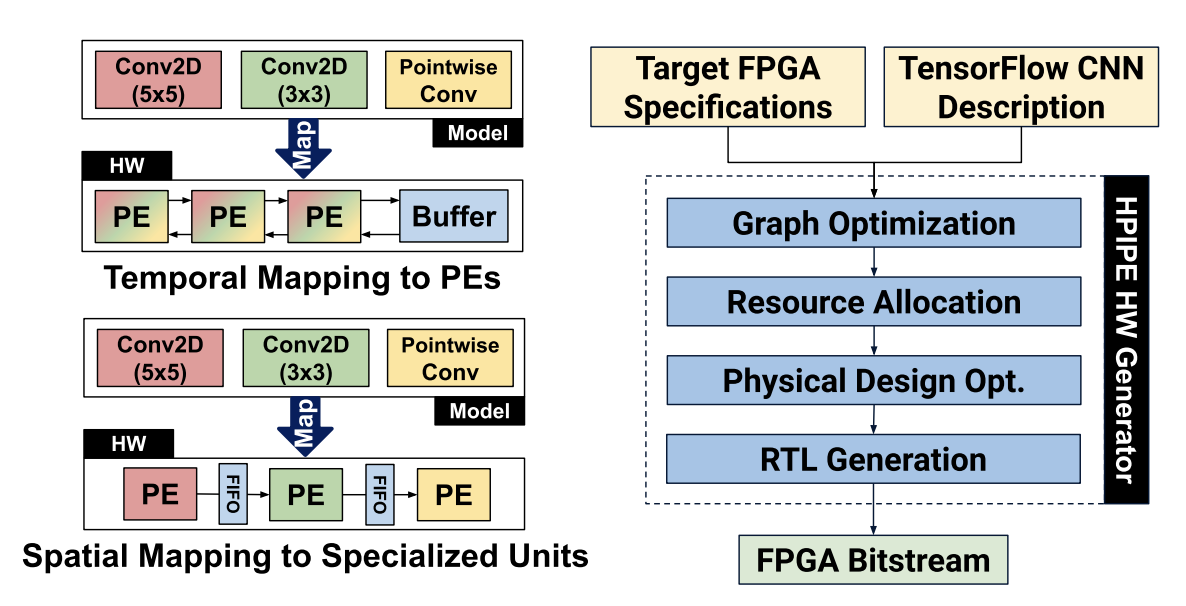
\includegraphics[width=0.75\linewidth]{assets/fpga_5.png}
    \caption{Ánh xạ theo thời gian của các mô hình học sâu (DL) lên một mảng các đơn vị xử lý (PEs) (góc trên bên trái) so với việc xây dựng các khối tính toán tùy chỉnh theo từng lớp như trong HPIPE (góc dưới bên trái) và tổng quan về quy trình tạo phần cứng của HPIPE (bên phải).}
    \label{fig:fpga_5}
\end{figure}

HPIPE là một trình biên dịch chuyên ngành tạo ra các bộ tăng tốc FPGA dựa trên luồng dữ liệu được xếp lớp theo dạng pipeline cho các CNN có trọng số cố định, trong đó toàn bộ trọng số được lưu trữ trong bộ nhớ SRAM on-chip. HPIPE xây dựng một mô-đun xử lý độc nhất cho mỗi lớp của CNN và nối các mô-đun đó với nhau qua các FIFO không nhạy với độ trễ. Nó còn khai thác tính hiếm của trọng số bằng cách bỏ qua các phép tính với trọng số bằng 0 không hiệu quả, giúp giảm đáng kể yêu cầu bộ nhớ on-chip và cải thiện hiệu suất bằng cách thực hiện ít phép toán hơn. So với cách tiếp cận dùng chung cho tất cả các lớp (trong đó cùng một mảng các phần tử xử lý được sử dụng cho mọi lớp – xem hình \ref{fig:fpga_5} bên trái), các mô-đun tùy chỉnh riêng cho từng lớp của HPIPE cho phép sử dụng tài nguyên tính toán tốt hơn và tận dụng được khả năng song song của pipeline, khi tất cả các lớp của CNN được thực thi đồng thời trên các phần khác nhau của một ảnh hoặc trên các ảnh khác nhau. Như được minh họa ở \ref{fig:fpga_5} bên phải, trình biên dịch HPIPE nhận đầu vào là mô tả CNN bằng TensorFlow và các thông số kỹ thuật của FPGA mục tiêu. Sau đó, nó thực hiện một loạt các tối ưu hóa trên đồ thị luồng dữ liệu của CNN (ví dụ: gộp các lớp để cài đặt hiệu quả hơn). Tiếp theo, nó phân bổ tài nguyên phần cứng cho từng lớp nhằm cân bằng thông lượng của tất cả các lớp pipeline và tối đa hóa hiệu suất tổng thể. Trình biên dịch HPIPE còn thực hiện các tối ưu hóa thiết kế vật lý, xét đến bố cục không gian của các mô-đun lớp và triển khai các cấu trúc kết nối tối ưu cho khả năng fanout cao và kết nối đường dài, giúp đạt được tần số hoạt động cao. Cuối cùng, nó tạo ra các tệp RTL của bộ tăng tốc và tệp khởi tạo bộ nhớ để lưu các trọng số của CNN trong bộ nhớ on-chip; RTL này sau đó được biên dịch thành bitstream bằng các công cụ CAD FPGA truyền thống.

Sử dụng FPGA Intel Stratix 10 GX2800 – FPGA 14nm monolithic (single die) lớn nhất hiện có, HPIPE đã vượt trội hơn tất cả các bộ tăng tốc CNN trên FPGA cùng thế hệ. Nó còn có thể đạt được thông lượng ResNet-50 cao hơn gấp 4 lần với cùng độ trễ (dưới 1ms) so với suy luận theo lô 1 mẫu trên GPU Nvidia V100, trên một công nghệ chế tạo tương đương (12nm). Khi tăng kích thước lô, GPU có thể tăng hiệu quả sử dụng nhưng độ trễ cũng tăng; HPIPE vẫn đạt được thông lượng cao hơn 1.4 lần nhưng với độ trễ thấp hơn 2.2 lần so với GPU V100 chạy với lô 8 mẫu. Điều này cho thấy lợi thế của FPGA đối với các ứng dụng yêu cầu độ trễ thấp; tính linh hoạt của FPGA cho phép tùy chỉnh cực đoan cho từng mô hình, mang lại hiệu quả vượt trội so với những chi phí phụ thuộc vốn có của tính tái cấu hình. Việc tạo ra phần cứng tự động từ mô tả mô hình cấp cao loại bỏ nhu cầu có chuyên môn thiết kế FPGA, nhưng vẫn đòi hỏi thời gian biên dịch bitstream mới cho mỗi mô hình khác nhau khi triển khai.

\textbf{2) Ví dụ Overlay (NPU):}

\begin{figure} [!h]
    \centering
    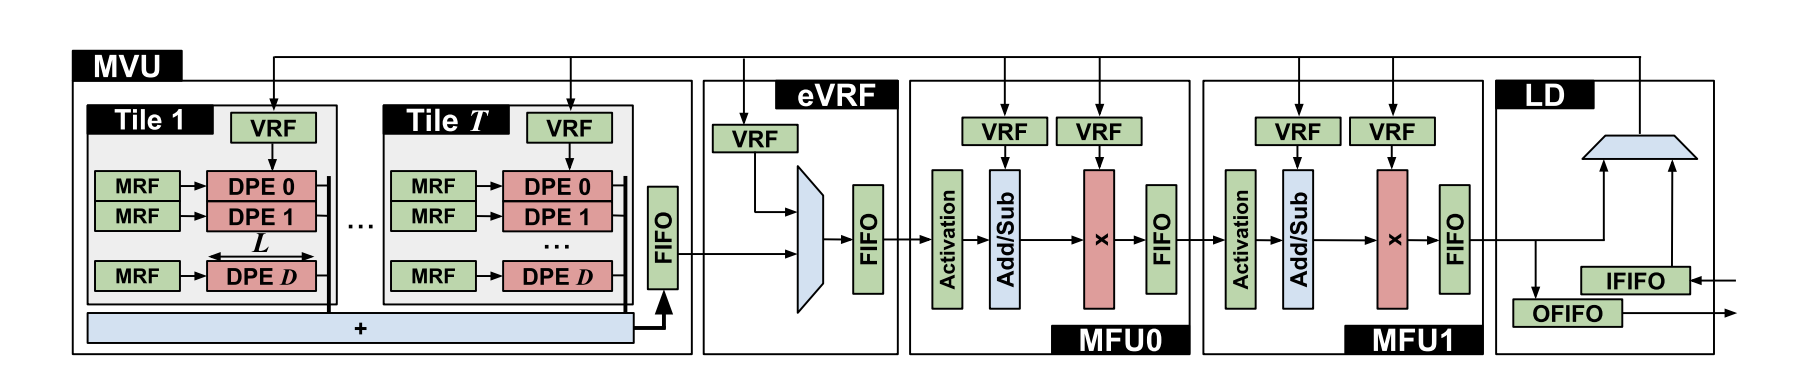
\includegraphics[width=0.75\linewidth]{assets/fpga_6.png}
    \caption{Kiến trúc overlay của NPU}
    \label{fig:fpga_6}
\end{figure}

Bộ xử lý nơ-ron (NPU) là một kiến trúc bộ xử lý dạng tập lệnh rất dài (VLIW) nhằm mục tiêu suy luận DL theo lô 1 mẫu với độ trễ thấp cho các mô hình không tái sử dụng dữ liệu (tức là bị giới hạn bởi bộ nhớ), chẳng hạn như các loại RNN và mạng perceptron đa lớp (MLP). Thiết kế overlay NPU dựa trên hai nguyên tắc chính. Đầu tiên, nó khai thác tính song song khổng lồ của các mô hình DL để giảm bớt chi phí năng lượng và diện tích của khả năng lập trình được bằng phần mềm; một lệnh VLIW thô sơ có thể kích hoạt thực hiện hàng nghìn phép toán, giống như một ví dụ cực đoan của kiến trúc máy tính tập lệnh phức tạp (CISC). Thứ hai, nó tùy chỉnh hệ thống bộ nhớ của bộ xử lý để tận dụng băng thông khổng lồ giữa các bộ nhớ on-chip phân tán của FPGA và các đơn vị tính toán, thực hiện tính toán gần bộ nhớ. Hệ thống bộ nhớ được quản lý tường minh (không sử dụng cache), sử dụng nhiều file thanh ghi khác nhau với mục đích cụ thể và từ dữ liệu rộng thay vì chỉ một nhóm chung, và nối trực tiếp nhiều phép toán giữa các đơn vị chức năng mà không cần truy cập file thanh ghi. Hình \ref{fig:fpga_6} cho thấy kiến trúc của overlay NPU, gồm năm đơn vị xâu chuỗi với độ thô chung sao cho đầu ra của một đơn vị cấp vào đơn vị tiếp theo. Đường ống bắt đầu với một đơn vị nhân ma trận - vector (MVU). MVU bao gồm $T$ ô tính toán, mỗi ô có $D$ động cơ tích chập (DPE) với $L$ lane nhân. Các toán hạng vector được phát sóng từ một file thanh ghi vector (VRF) tới tất cả các DPE trong một ô, trong khi các trọng số mô hình cố định được lấy từ các file thanh ghi ma trận (MRF). MVU được theo sau bởi một VRF ngoài (eVRF) cho phép bỏ qua MVU nếu lệnh không bắt đầu bằng phép nhân ma trận - vector. Phần còn lại của đường ống gồm hai đơn vị đa chức năng (MFU) thực hiện các phép toán từng phần tử của vector (ví dụ: hàm kích hoạt, phép cộng, phép nhân) và một đơn vị tải (loader) có thể ghi lại kết quả vào bất kỳ trạng thái kiến trúc bộ xử lý nào (tức là VRF) hoặc giao tiếp với các thành phần bên ngoài (ví dụ: giao diện mạng) qua các FIFO vào/ra. Các nhà phát triển ứng dụng DL mô tả các mô hình của họ bằng một tập con của giao diện lập trình Tensorflow Keras sau đó được biên dịch thành chuỗi lệnh VLIW của NPU để thực thi trên overlay FPGA.

Overlay NPU được triển khai trên FPGA Intel Stratix 10 GX2800 đạt được độ trễ lô 1 mẫu thấp hơn 2.7 lần so với GPU Nvidia V100 cho nhiều tải công việc RNN từ bộ sưu tập DeepBench khi sử dụng cùng độ chính xác fp32 như GPU. Khi sử dụng độ chính xác số nguyên 8-bit thân thiện hơn với FPGA, hiệu suất tăng lên đến 8.6 lần. Điều này cho thấy rằng một overlay FPGA chuyên ngành với kiến trúc và ISA tùy chỉnh có thể mang lại hiệu suất cao hơn nhiều so với các pipeline bộ xử lý chung của GPU và CPU, đồng thời vẫn cung cấp khả năng lập trình phần mềm tương tự.

\textbf{3) Ảnh hưởng của Các Cải tiến Kiến trúc FPGA cho DL:} \\
    Cả HPIPE và overlay NPU đều được thiết kế sao cho phù hợp nhất với kiến trúc cơ bản của FPGA. Ví dụ, cả hai đều tổ chức các đơn vị tính toán MAC cơ bản để sử dụng hiệu quả các khối xử lý tín hiệu số (DSP) tích hợp sẵn trong FPGA mục tiêu. HPIPE sử dụng các kết nối không lập trình được giữa các khối DSP để xây dựng các phép nhân tích chập theo dạng pipeline hiệu quả, với việc sử dụng tối thiểu logic lập trình và mạch định tuyến lập trình được của FPGA. Ngược lại, overlay NPU sử dụng một lượng nhỏ logic mềm để thực hiện hiệu chỉnh sau phép nhân, cho phép đóng gói mật độ bốn phép nhân số nguyên 8-bit vào trong hai phép nhân số nguyên 18-bit có sẵn trong một khối DSP trên FPGA Intel Stratix 10. Những tối ưu hóa này nhằm tăng cường hiệu suất DL với giả định rằng kiến trúc FPGA không thay đổi. Tuy nhiên, kiến trúc FPGA đã không ngừng tiến hóa để phù hợp hơn với các trường hợp sử dụng và thị trường mục tiêu trong suốt ba thập kỷ qua. Khi DL trở thành tải công việc chủ đạo, nhiều cải tiến kiến trúc FPGA hướng đến DL đã được đề xuất trong vài năm gần đây.
    
    Một ví dụ về cải tiến kiến trúc FPGA hướng DL (được trình bày chi tiết hơn ở phần sau của bài báo) là thay thế các khối DSP truyền thống bằng các khối tensor tối ưu hóa cho DL trên FPGA Intel Stratix 10 NX. Các khối tensor này thay thế các chế độ hoạt động và độ chính xác của khối DSP cũ bằng các chế độ hướng DL có thể thực hiện nhiều phép nhân số nguyên 8-bit và 4-bit hơn cho mỗi khối. Bằng cách hạn chế các mẫu dữ liệu đầu vào và đầu ra nhằm đạt được thông lượng đỉnh (và tránh việc bổ sung các mạch định tuyến lập trình được đắt tiền), các khối tensor này đạt được diện tích tương đương với khối DSP truyền thống. Cả HPIPE và overlay NPU đã được nâng cấp để sử dụng các FPGA tối ưu hóa DL mới với các khối tensor, mang lại hiệu suất tăng đáng kể. Đối với HPIPE, các khối tensor cải thiện thông lượng suy luận từ 6,000 lên 29,400 suy luận mỗi giây theo lô 1 mẫu cho CNN MobileNet-V2 so với FPGA sử dụng khối DSP truyền thống. So với GPU Nvidia V100 (có kích thước die hơn 1.5 lần so với FPGA Intel Stratix 10 NX), HPIPE sử dụng khối tensor đạt được thông lượng cao hơn 17 lần và độ trễ thấp hơn 3 lần với lô 1 mẫu, hoặc thông lượng cao hơn 1.3 lần và độ trễ thấp hơn 29 lần với lô 128 mẫu. Mặt khác, hiệu suất của overlay NPU được cải thiện 3.5 lần khi sử dụng các khối tensor so với khối DSP truyền thống, dẫn đến hiệu suất cao hơn 11 lần so với GPU V100. Hai ví dụ này cho thấy rõ tác động đáng kể của các cải tiến kiến trúc chuyên biệt cho DL đối với hiệu suất suy luận trên FPGA. Trong bài báo này, chúng tôi trình bày nhiều cải tiến kiến trúc như vậy từ cả công nghiệp và học thuật với mục tiêu chung: làm cho FPGA trở nên tốt hơn trong việc tăng tốc DL.

\subsection{Các Thành phần Chính của Kiến trúc FPGA và Cơ hội Tối ưu hóa cho Tính toán DL}
Trong phần này, chúng tôi tóm tắt các thành phần cơ bản của kiến trúc FPGA và nêu bật các cơ hội để tối ưu hóa các thành phần này cho các tác vụ tính toán DL. Đối với khảo sát toàn diện về các nguyên tắc thiết kế và sự tiến hóa của kiến trúc FPGA, độc giả vui lòng tham khảo.

\subsubsection{Logic Lập trình được và Định tuyến}

\begin{figure}[!h]
    \centering
    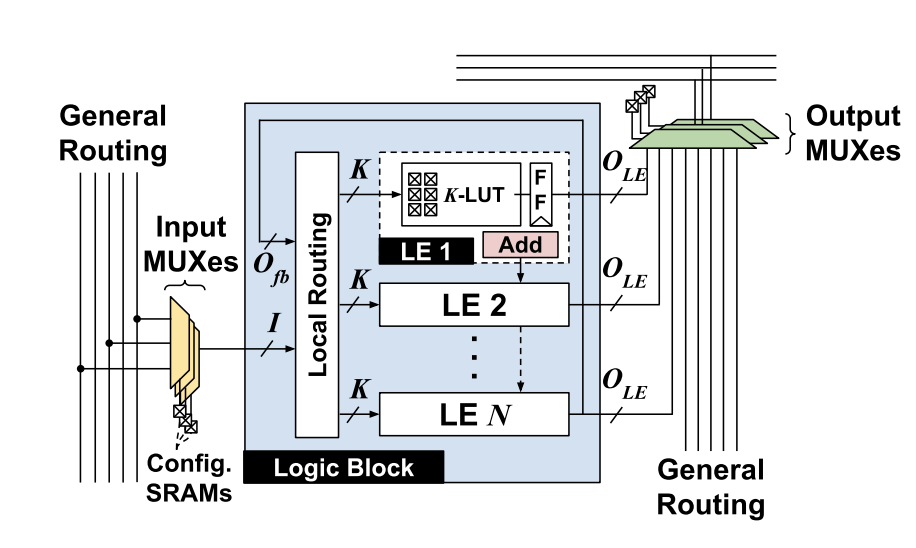
\includegraphics[width=0.75\linewidth]{assets/fpga_7.png}
    \caption{Khối logic (LB) và kiến trúc định tuyến.}
    \label{fig:fpga_7}
\end{figure}

Các khối logic lập trình được (LBs) là nguồn tài nguyên dồi dào nhất của một FPGA. Một LB là tập hợp của $N$ phần tử logic (LEs) cùng với các kết nối cục bộ. Như minh họa trong hinhf \ref{fig:fpga_7}, các bộ định tuyến lập trình được điều khiển bởi SRAM (các MUX định tuyến) nối các dây dẫn định tuyến chung với nhau cũng như với các đầu vào/đầu ra của LB.

Ở dạng đơn giản nhất, mỗi LE kết hợp một bảng tra cứu (LUT) dựa trên SRAM với $K$ đầu vào và một flip-flop có khả năng bypass, cho phép thực hiện bất kỳ hàm logic Boolean nào với $K$ đầu vào (có thể đăng ký). Nhiều kiến trúc FPGA hiện đại còn cho phép “phân tách” các LE để thực hiện hai hàm logic, mỗi hàm sử dụng tối đa $K-1$ đầu vào – sao cho tổng số đầu vào không vượt quá số lượng đầu vào mà hệ thống định tuyến cục bộ cung cấp cho một LE. Các LE cũng bao gồm mạch chuyên dụng (hộp màu hồng trong hình \ref{fig:fpga_7}) để hiện thực các phép cộng, một thành phần quan trọng trong nhiều thiết kế FPGA và rất phổ biến trong các bộ tăng tốc DL.

Hầu hết các FPGA thương mại từ AMD và Intel đều triển khai các LB với khoảng 8 đến 10 LE, mỗi LE có 6 đầu vào (tức là $N = 8\text{–}10$, $K = 6$). Một điểm khác biệt quan trọng là mỗi LE trong FPGA của Intel bao gồm mạch chuyên dụng để thực hiện phép cộng 2-bit, trong khi mỗi LE của AMD chỉ thực hiện được 1-bit cộng. Các LB (cùng với các thành phần khác của FPGA và IO) được bao quanh bởi hệ thống định tuyến lập trình được linh hoạt, bao gồm các bộ MUX được điều khiển bằng SRAM nối đầu ra của các khối với nhau (các MUX màu xanh lá trong hình \ref{fig:fpga_7}) và nối các dây định tuyến với các đầu vào của LB (các MUX màu vàng trong hình \ref{fig:fpga_7}). Các bộ MUX này chiếm hơn 50\% diện tích của một ô logic (LB và hệ thống định tuyến của nó).

Vì việc thêm đầu vào/đầu ra cho LB hoặc khối cứng đòi hỏi thêm các bộ MUX định tuyến, nên các thay đổi kiến trúc tăng số lượng đầu ra vào của một khối cần được cân nhắc kỹ lưỡng giữa lợi ích chức năng và chi phí diện tích.

Logic lập trình được và hệ thống định tuyến là chìa khóa của khả năng lập trình ở mức bit của FPGA, cho phép triển khai bất kỳ chức năng nào bằng cách thiết lập các cell cấu hình của LUT và các bộ định tuyến SRAM. Đối với DL, các đơn vị MAC với độ chính xác thấp thường được hiện thực hóa bằng cách sử dụng LUT, flip-flop và mạch cộng chuyên dụng trong các LE. Ví dụ, bộ tăng tốc DL dựa trên FPGA Microsoft Brainwave đã hiện thực các đơn vị tính toán theo định dạng số thực 8-bit tùy chỉnh (msfp8) trong logic lập trình được. Định dạng số thực này, nhấn mạnh dải động hơn độ chính xác, cho mật độ MAC cao hơn gấp 2.9 lần so với các đơn vị int8 truyền thống và mang lại độ chính xác suy luận tương đương với số thực 32-bit (fp32). Khi một chút giảm độ chính xác được chấp nhận, các MAC nhị phân với độ chính xác thấp (hiện thực thông qua các phép XNOR và popcount) cũng có thể được sử dụng, cho ra các đơn vị tính toán nhỏ gọn và hiệu quả. Tuy nhiên, vì các phép toán với bề rộng bit hẹp là thế mạnh của FPGA nhưng các LB hiện nay được kiến trúc từ trước khi DL bùng nổ, nên vẫn còn khả năng cải tiến thêm về hiệu quả MAC.

\textbf{Cơ hội 1:} Tăng cường kiến trúc khối logic để hiện thực các phép nhân và cộng với độ chính xác bit hẹp hiệu quả hơn có thể mang lại lợi ích đáng kể cho tăng tốc DL với độ chính xác thấp.

\textbf{Khối Xử lý Tín hiệu Số (DSP)}

Vì các tải công việc DL chủ yếu dựa vào các phép MAC, các khối DSP đóng vai trò quan trọng trong việc hiện thực các bộ tăng tốc DL trên FPGA. Các khối DSP là các khối cứng kiểu ASIC được nhúng trong cấu trúc FPGA, chuyên hiện thực các phép nhân và cộng, nhưng được thiết kế với mức độ lập trình nhất định để tăng khả năng sử dụng trong nhiều thiết kế FPGA mà vẫn giữ được hiệu suất kiểu ASIC.

Ví dụ, các khối DSP trong họ FPGA Intel Arria 10 và Stratix 10 có mạch điều khiển cấu hình được để thực hiện các phép nhân với độ chính xác khác nhau (ví dụ: một phép nhân int27 hoặc hai phép nhân int18) cùng với các bộ cộng trước nhân tùy chọn, bộ cộng/accumulator sau nhân, các thanh ghi pipeline có thể bỏ qua và các dây định tuyến chuyên dụng nối giữa các khối DSP trong cùng một cột. Các khối DSP này ban đầu được thiết kế cho các ứng dụng truyền thông không dây và lọc tín hiệu, nên chúng hỗ trợ sẵn các độ chính xác số học phổ biến trong lĩnh vực đó (ví dụ: phép nhân 27×27 và 18×18 trên FPGA Intel, 27×18 trên FPGA AMD). Tuy nhiên, khi dùng để hiện thực các đơn vị MAC cho DL, các độ chính xác này thường vượt mức yêu cầu suy luận DL, dẫn đến việc sử dụng không tối đa các tính năng của khối DSP (hay lãng phí diện tích silicon do khối DSP được thiết kế vượt mức cần thiết cho DL).

\textbf{Cơ hội 2:} Thêm mạch điều khiển cấu hình chi phí thấp nhằm phân chia các bộ nhân bên trong khối DSP thành các bộ nhân có độ chính xác thấp hơn (vẫn đảm bảo tương thích ngược) có thể tăng hiệu suất DL.

Ngoài ra, các khối DSP còn tích hợp các tính năng hữu ích cho các ứng dụng FPGA truyền thống như truyền thông không dây. Ví dụ, khối DSP trên FPGA Intel Stratix 10 có một ngân hàng hệ số hằng số nhỏ và các thanh ghi/xung nối tiếp đầu vào để hiện thực các bộ lọc FIR hiệu quả. Các tính năng này tiêu tốn diện tích silicon nhưng lại ít hữu ích cho tính toán DL; việc thay thế chúng bằng các tính năng tập trung vào DL có thể cải thiện hiệu quả tính toán DL, mặc dù có thể mất đi tính tương thích với các khối DSP truyền thống.

\textbf{Cơ hội 3:} Thay thế các khối DSP ban đầu thiết kế cho truyền thông không dây bằng các khối chuyên dụng hướng DL mới có thể tăng mật độ tính toán và hiệu quả của FPGA cho các tác vụ DL.

\textbf{Bộ Nhớ On-Chip (BRAMs)}

FPGA còn bao gồm một số lượng lớn các khối bộ nhớ SRAM on-chip, thường gọi là block RAMs (BRAMs). Những BRAM này (hơn 10.000 khối trong các FPGA hiện đại) được phân bố theo cột khắp cấu trúc FPGA, như minh họa ở Hình \ref{fig:fpga_10}. Các thế hệ mới nhất của FPGA Intel có một loại BRAM duy nhất với dung lượng 20Kb, trong khi FPGA của AMD có các BRAM 36Kb cũng như các RAM lớn hơn nhưng ít phổ biến hơn với dung lượng 288Kb (thường gọi là Ultra RAMs hoặc URAMs). Lõi của các BRAM là mảng SRAM có kích thước cố định kèm theo mạch ngoại vi truyền thống cho các hoạt động đọc/ghi như bộ giải mã hàng, bộ khuếch đại tín hiệu và bộ driver ghi.

Tương tự như khối DSP, các BRAM bao gồm mạch cấu hình chi phí thấp trong mạch ngoại vi để cho phép triển khai các bộ đệm với độ rộng/độ sâu khác nhau (ví dụ: bộ đệm hẹp và sâu so với bộ đệm nông và rộng) và số lượng cổng tùy thuộc vào nhu cầu ứng dụng. Ví dụ, bằng cách thiết lập một vài cell cấu hình SRAM, một BRAM 20Kb có thể được sử dụng như ROM, RAM một cổng, hoặc RAM hai cổng với tổ chức dữ liệu như 1b×16K, 2b×8K, 4b×4K, 8b×2K, 16b×1K, 32b×512 hoặc 40b×512.

Tất cả các BRAM có thể được truy cập song song, cung cấp băng thông bộ nhớ on-chip khổng lồ (trên mức petabit/giây) với chỉ một đến hai chu kỳ trễ truy cập. Ngoài ra, chúng có thể được điều khiển độc lập và kết nối trực tiếp với các đơn vị tính toán bằng cách tận dụng tính linh hoạt của hệ thống định tuyến lập trình được của FPGA. Những tính năng này rất hữu ích cho các tác vụ DL yêu cầu tính toán song song với độ trễ thấp. Tuy nhiên, với nhu cầu ngày càng tăng để đưa tính toán càng gần dữ liệu nhằm đạt hiệu quả cao hơn, hàng nghìn khối bộ nhớ on-chip của FPGA có tiềm năng thực hiện thêm các chức năng tính toán thay vì chỉ lưu trữ dữ liệu cho các đơn vị tính toán trong LB và DSP.

\textbf{Cơ hội 4:} Với những tiến bộ trong công nghệ tính toán trong bộ nhớ, việc tăng cường BRAM với khả năng tính toán ngay bên trong có thể cung cấp hàng nghìn đơn vị tính toán song song trên FPGA với chi phí tương đối thấp.

\textbf{Interposers}

Vì FPGA thường là người tiên phong trong việc áp dụng các công nghệ quy trình mới, việc tạo ra FPGA lớn với một die silicon đơn thể thường gặp vấn đề về năng suất (do lỗi sản xuất) đặc biệt là trong giai đoạn đầu của quy trình. Để khắc phục điều này, nhiều FPGA hiện đại sử dụng công nghệ interposer thụ động để tích hợp nhiều die silicon nhỏ hơn vào cùng một gói. Điều này không chỉ cải thiện năng suất sản xuất mà còn cho phép phát triển phần cứng linh hoạt hơn bằng cách kết hợp lớp FPGA với các chiplet được sản xuất sẵn, thực hiện các chức năng khác nhau và (có thể) sử dụng các quy trình khác nhau, tạo thành một hệ thống hoàn chỉnh trong một gói.

\begin{figure} [!h]
    \centering
    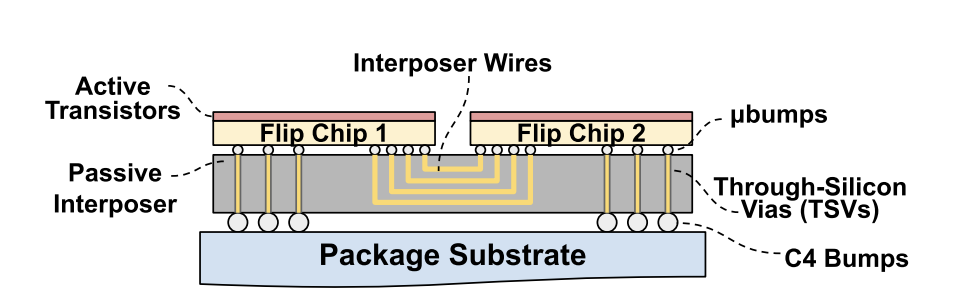
\includegraphics[width=0.75\linewidth]{assets/fpga_8.png}
    \caption{Công nghệ interposer thụ động}
    \label{fig:fpga_8}
\end{figure}

Như minh họa ở hình \ref{fig:fpga_8}, một interposer là một die silicon với các lớp kim loại thông thường nhưng không có transistor hoạt động nào (do đó gọi là interposer thụ động). Lớp kim loại trên cùng của interposer có thể kết nối với lớp kim loại trên cùng của nhiều die được lật lên trên nó thông qua các bóng hàn (microbumps) có mật độ cao (thường cách nhau vài chục µm), cung cấp mật độ cao các đường định tuyến giữa các chip trong cùng một gói.

FPGA của AMD đã sử dụng công nghệ này từ dòng 7-series 28nm để tích hợp nhiều die FPGA, được trình bày cho người dùng như một FPGA lớn với nhiều vùng logic siêu lớn (SLRs). FPGA của Intel cũng sử dụng công nghệ tương tự, được gọi là cầu liên kết đa die nhúng (EMIB), để tích hợp một die FPGA với nhiều chiplet truyền thông hoặc bộ nhớ băng thông cao (HBM) từ dòng Stratix 10 14nm. Những công nghệ này cho phép tạo ra nhiều biến thể thiết bị cho các thị trường khác nhau, tùy thuộc vào các chip ASIC chuyên dụng tích hợp cùng với FPGA trong cùng một gói. Ngay cả khi các mô hình DL tiên tiến thay đổi nhanh chóng, các phép toán MAC song song – thành phần cốt lõi của hầu hết các mô hình – có thể được chuyển giao cho một chiplet ASIC hiệu quả. Trong trường hợp này, FPGA trong cùng một gói có thể cung cấp tính linh hoạt cần thiết cho bất kỳ sự thay đổi mô hình DL nào và các giao diện IO đa dạng cho phần còn lại của hệ thống.

\textbf{Cơ hội 5:} Tích hợp FPGA với các ASIC chuyên dụng cho DL bằng công nghệ gói tiên tiến có thể kết hợp những ưu điểm của cả hai: tính linh hoạt của FPGA cho các phần tùy chỉnh của hệ thống và hiệu quả của ASIC cho các chức năng chung.

\textbf{Mạng lưới trên Chip (NoC) và Bộ Tăng tốc Nhúng}

Gần đây, các thiết bị tăng tốc có khả năng tái cấu hình vượt ra ngoài FPGA (RADs) đã xuất hiện. Một ví dụ điển hình là kiến trúc AMD Versal, kết hợp lớp FPGA với các lõi xử lý tổng quát và một mảng bộ xử lý vector có thể lập trình được bằng phần mềm trong một thiết bị duy nhất. Tất cả các thành phần này được kết nối qua một mạng lưới trên chip chuyển gói (NoC) nhằm giao tiếp hệ thống một cách hiệu quả. Mạng NoC cho phép tích hợp nhanh chóng và dễ dàng các hệ thống kết hợp các IP thiết kế mềm hiện thực trên FPGA cùng với các bộ tăng tốc nhúng chuyên dụng có độ thô cao. Kiến trúc AMD Versal là một ví dụ tiêu biểu, mở ra một không gian rộng lớn cho các thiết bị tính toán tái cấu hình mới có thể hỗ trợ tăng tốc DL hiệu quả.

\textbf{Cơ hội 6:} Khám phá không gian thiết kế của các thiết bị RAD hướng DL mới, kết hợp những đặc tính độc đáo của FPGA với các bộ tăng tốc DL dạng coarse-grained hiệu quả hơn.

\subsection{Khám khá kiến trúc FPGA cho DL}
\subsubsection{Công cụ và Bộ Benchmark}

\begin{figure} [!h]
    \centering
    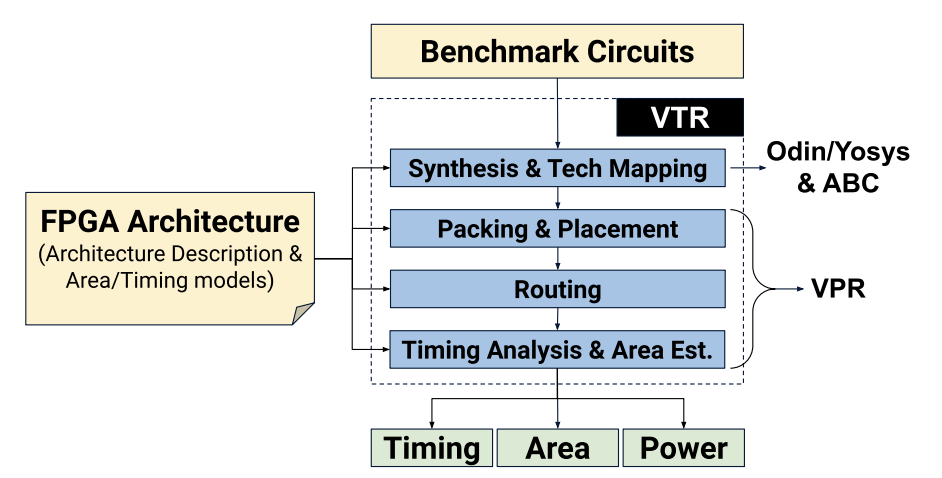
\includegraphics[width=0.75\linewidth]{assets/fpga_9.png}
    \caption{Các thành phần chính để khám phá kiến trúc FPGA: mạch chuẩn, mô tả kiến trúc và luồng CAD có thể định hướng lại (retargettable).}
    \label{fig:fpga_9}
\end{figure}
Hình \ref{fig:fpga_9} minh họa quy trình thường được sử dụng để đánh giá các thay đổi kiến trúc FPGA. Ở trung tâm của quy trình này là một công cụ CAD FPGA có khả năng tái định hướng (retargettable) cho phép tổng hợp, đặt vị trí và định tuyến một tập hợp các thiết kế benchmark trên một loạt các kiến trúc FPGA đầu vào. Các kiến trúc sư sau đó có thể đánh giá các kiến trúc ứng viên bằng cách so sánh các chỉ số thời gian, diện tích và công suất được báo cáo bởi các công cụ CAD.

Verilog-to-Routing (VTR) là một quy trình mã nguồn mở được sử dụng rộng rãi trong nghiên cứu kiến trúc FPGA và CAD. VTR kết hợp nhiều công cụ như ODIN hoặc Yosys cho tổng hợp Verilog, ABC cho tối ưu hóa logic và ánh xạ công nghệ, VPR cho đóng gói, đặt vị trí và định tuyến, và Tatum cho phân tích thời gian tĩnh. VTR nhận đầu vào là một tệp XML mô tả kiến trúc FPGA, bao gồm tổ chức cấp cao của FPGA (ví dụ: số lượng và loại khối, phân bố độ dài đoạn dây, kích thước cụm logic và phần tử logic), các chi tiết vi kiến trúc (ví dụ: chế độ hoạt động của DSP và BRAM, số học cứng trong các khối logic, mẫu của khối chuyển mạch) cũng như các thông số triển khai mạch cấp transistor (ví dụ: độ trễ và diện tích của các công tắc/dây dẫn). Các công cụ như COFFE tự động hóa thiết kế và mô hình hóa cấp transistor của mạch FPGA và tạo ra các tham số độ trễ, diện tích của các thành phần khác nhau để đưa vào tệp mô tả kiến trúc FPGA của VTR.

Việc tối ưu hóa kiến trúc FPGA cũng đòi hỏi phải có các thiết kế benchmark bao phủ nhiều trường hợp sử dụng trong các miền ứng dụng mục tiêu. Thông thường, các nhà cung cấp FPGA đã biên soạn kỹ lưỡng các bộ benchmark độc quyền đại diện cho các trường hợp sử dụng của khách hàng. Cũng có một số bộ benchmark mã nguồn mở thuộc học thuật như các mạch MCNC cổ điển, bộ VTR và bộ Titan23 được sử dụng phổ biến trong nghiên cứu kiến trúc FPGA và CAD. Mặc dù các nghiên cứu FPGA học thuật ban đầu sử dụng các mạch MCNC, nhưng chúng nay quá nhỏ (chỉ hàng nghìn logic primitives) và đơn giản (chỉ có IO và logic) để đại diện cho các ứng dụng FPGA hiện đại. Các bộ benchmark VTR và đặc biệt là Titan có quy mô và độ phức tạp lớn hơn, làm cho chúng trở nên đại diện hơn. Tuy nhiên, không bộ benchmark nào trong số này chứa các thiết kế FPGA đại diện cho miền DL. Bộ benchmark Koios đã được giới thiệu nhằm khắc phục khoảng trống này. Nó bao gồm 40 mạch DL với nhiều kích thước, kiểu triển khai, mô hình nơ-ron, độ chính xác số và các đặc tính mạch khác nhau. Ngoài ra, bộ Koios còn giới thiệu một phương pháp tạo ra các mạch tổng hợp (synthetic hoặc proxy) có đặc điểm tương tự như các mạch DL thực tế. Các bộ benchmark Koios được mở nguồn và tích hợp vào quy trình VTR, từ đó cho phép khám phá các kiến trúc FPGA được tối ưu hóa đặc biệt cho DL.

\subsubsection{Phương pháp Đánh giá} 
Trong phần này, chúng tôi giải thích phương pháp chung để đánh giá các ý tưởng kiến trúc FPGA mới sử dụng các công cụ và bộ benchmark đã được giới thiệu ở phần trên. Phương pháp tương tự cũng được sử dụng để đánh giá lợi ích và chi phí của hầu hết các cải tiến kiến trúc mạch FPGA được thảo luận trong bài báo này.

Một cải tiến kiến trúc FPGA phổ biến cho một miền mục tiêu cụ thể là bổ sung một loại khối cứng mới (hoặc thay đổi khối hiện có) vào mạch FPGA nhằm hiện thực hiệu quả các chức năng chung trong các thiết kế ứng dụng của miền đó. Ví dụ, đối với miền DL, một kiến trúc sư FPGA có thể đánh giá việc thêm các bộ xử lý tích chập cứng vào mạch FPGA. Điều này liên quan đến nhiều cân nhắc thiết kế và đặt ra các câu hỏi: diện tích die FPGA bao nhiêu nên được dành cho các bộ xử lý tích chập này? Chúng cần linh hoạt đến mức nào? Chúng có chỉ thực hiện tích chập hay có thể được cấu hình lại để thực hiện các phép toán khác và ứng dụng cho nhiều trường hợp khác nhau? Việc thêm chúng có ảnh hưởng như thế nào đến nhu cầu của hệ thống định tuyến lập trình được? Chúng cải thiện hiệu suất ứng dụng mục tiêu tổng thể lên bao nhiêu và với chi phí như thế nào đối với các miền ứng dụng khác?

Để trả lời các câu hỏi này, kiến trúc sư trước tiên viết một mô tả RTL cho khối cứng mới được đề xuất (ví dụ: bộ xử lý tích chập). Mô tả này trình bày chức năng chính xác theo chu kỳ của khối cũng như các chế độ hoạt động có thể lập trình lại của nó. Sau đó, họ tiến hành đánh giá cấp mạch bằng cách sử dụng các công cụ như COFFE. Mạch FPGA bao gồm cả các thành phần cell tiêu chuẩn (ASIC) và các thành phần thiết kế toàn tùy chỉnh (với transistor và layout được tối ưu hóa bằng tay); COFFE sẽ mô hình hóa và đánh giá cả hai loại. Chức năng của khối cứng được hiện thực bằng các công cụ EDA cho ASIC cell tiêu chuẩn, trong khi giao diện đến hệ thống định tuyến lập trình được hiện thực thông qua thiết kế tùy chỉnh hoàn toàn và mô hình SPICE. Kết quả của bước này là các mô hình về diện tích, độ trễ và tiêu thụ điện năng của khối cứng được đề xuất.

Các mô hình này sau đó được tích hợp vào quy trình CAD FPGA (ví dụ: VTR) để thực hiện đánh giá cấp kiến trúc bằng cách ánh xạ một tập hợp các mạch benchmark đại diện (ví dụ: bộ Koios) lên kiến trúc FPGA bao gồm khối cứng mới. Việc ánh xạ có thể được thực hiện bằng cách sửa đổi benchmark để khởi tạo trực tiếp một thể hiện của khối mới hoặc mở rộng các công cụ tổng hợp để tự động trích xuất các thành phần netlist của mạch và ánh xạ chúng vào khối mới. Bước cuối cùng này đánh giá việc sử dụng tài nguyên, độ trễ và khả năng định tuyến của các benchmark trên kiến trúc FPGA được đề xuất. Các cải tiến đối với các khối logic lập trình được và BRAM có thể được đánh giá theo phương pháp tương tự, ngoại trừ việc lõi của chúng cũng được thiết kế và bố trí tùy chỉnh thay vì được hiện thực bằng cell ASIC tiêu chuẩn.

\subsubsection{Phân loại Các Cải tiến Kiến trúc FPGA cho DL}

\begin{figure} [!h]
    \centering
    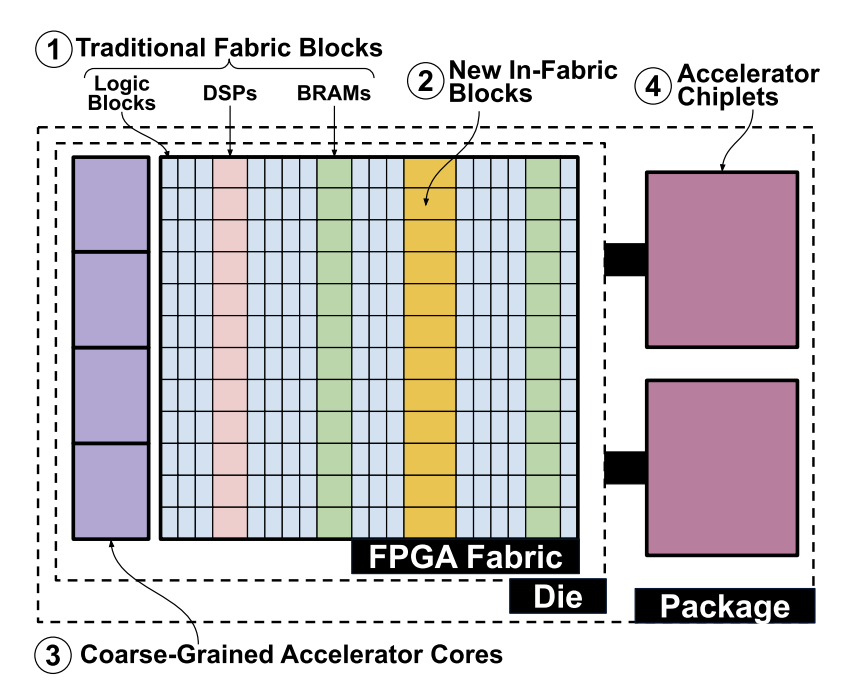
\includegraphics[width=0.75\linewidth]{assets/fpga_10.png}
    \caption{Phân loại các cải tiến kiến trúc FPGA cho DL}
    \label{fig:fpga_10}
\end{figure}
Trong phần tiếp theo ta sẽ trình bày một số cải tiến kiến trúc FPGA hướng DL từ cả học thuật và công nghiệp. hình \ref{fig:fpga_10} minh họa phân loại các đề xuất này, bao gồm:
\begin{enumerate}
    \item Tối ưu hóa các khối mạch FPGA truyền thống (ví dụ: LB, DSP, BRAM).
    \item Giới thiệu các khối cứng DL đặc thù nội mạch (ví dụ: các khối tensor).
    \item Tích hợp chặt chẽ các bộ tăng tốc DL dạng coarse-grained trên cùng một die với mạch FPGA (ví dụ: các engine AI của AMD).
    \item Tích hợp FPGA với các chiplet DL khác trong cùng một gói.
\end{enumerate}

\subsection{Tăng cường các thành phần FPGA}
\subsubsection{Khối Logic (LBs)}
Như đã thảo luận ở phần trước, nhiều nghiên cứu cho thấy các mô hình DL có thể được lượng tử hóa xuống các độ chính xác thấp với mất mát độ chính xác ít hoặc không đáng kể trong suy luận. Các phép toán MAC với số nguyên hẹp (ví dụ: int8, int4) hiện nay được hỗ trợ tự nhiên trong nhiều bộ tăng tốc DL thương mại. Ngoài ra, các định dạng số thực với độ chính xác thấp mới như fp8 cũng đang được chuẩn hóa và dự kiến sẽ được hỗ trợ trong thế hệ FPGA tiếp theo cho DL.

FPGA cung cấp sự linh hoạt để hiện thực bất kỳ độ chính xác số học nào trực tiếp trong phần cứng nhờ khả năng lập trình ở mức chi tiết của các LB. Vì số lượng logic sử dụng cho một bộ nhân tăng theo hàm bậc hai với độ chính xác, việc cắt giảm độ chính xác xuống mức tối thiểu có thể mang lại tiết kiệm diện tích lớn. Các LB là nguồn tài nguyên dồi dào nhất trong một FPGA, vì vậy những thay đổi kiến trúc giúp tăng hiệu quả hiện thực các bộ nhân số có độ chính xác thấp sẽ có tác động cao đến các ứng dụng DL.
\begin{figure} [!h]
    \centering
    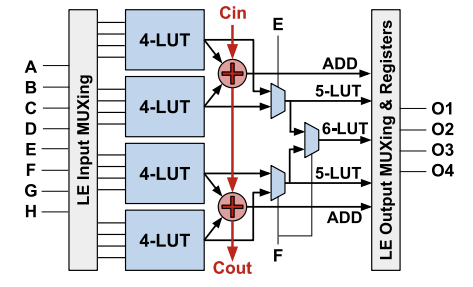
\includegraphics[width=0.75\linewidth]{assets/fpga_11.png}
    \caption{Kiến trúc của một phần tử logic (Logic Element) tương tự như trong Intel Stratix 10 và Agilex.}
    \label{fig:fpga_11}
\end{figure}
Hình \ref{fig:fpga_11} cho thấy kiến trúc nội bộ của một LE hiện đại, tương tự như trong FPGA Intel Stratix 10 và Agilex. LE có 8 đầu vào riêng biệt và 4 đầu ra (có thể đăng ký), cùng với hai mạch cộng nối tiếp được cấp bởi bốn LUT 4 đầu vào. Do đó, mỗi LE có thể hiện thực bốn hàm logic 4 đầu vào kèm theo phép cộng 2-bit, hoặc hai hàm logic 5 đầu vào, hoặc một hàm logic 6 đầu vào nếu không vượt quá 8 đầu vào riêng biệt. Hình \ref{fig:fpga_12} minh họa cách ánh xạ phép nhân 4-bit vào kiến trúc LE này, trong đó các bit của hai toán hạng được biểu diễn bằng các hình dạng và màu sắc khác nhau. Bước đầu tiên của phép nhân là thực hiện phép AND giữa mỗi bit của một toán hạng với tất cả các bit của toán hạng kia, tạo ra các sản phẩm từng phần. Sau đó, các sản phẩm này được giảm qua một hoặc nhiều giai đoạn cộng để tạo ra kết quả cuối cùng. Điều này chỉ ra một nguồn lãng phí lớn: các LUT chủ yếu chỉ thực hiện các phép AND 2 đầu vào (hoặc chức năng truyền thẳng) để truy cập các mạch cộng, dẫn đến việc sử dụng chỉ một nửa khả năng của một LUT 4 đầu vào.

\begin{figure} [!h]
    \centering
    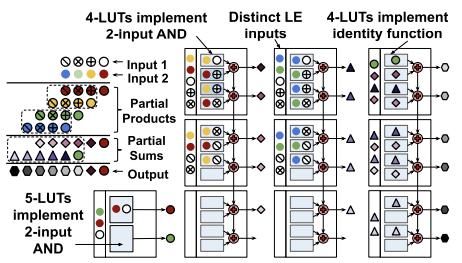
\includegraphics[width=0.75\linewidth]{assets/fpga_12.png}
    \caption{Ánh xạ phép nhân 4-bit vào các phần tử logic thông thường.}
    \label{fig:fpga_12}
\end{figure}

Người ta chỉ ra những điểm không hiệu quả này và đề xuất bốn cải tiến kiến trúc (tóm tắt trong Hình \ref{fig:fpga_13}) để khắc phục ở cả cấp LE và LB:
\begin{itemize}
    \item Đề xuất thứ nhất bổ sung một chuỗi cộng nối tiếp khác, nhận đầu vào từ hai đầu ra tổng của chuỗi hiện có và từ hai đầu vào độc lập, giúp hiện thực cây compressor mà không cần thêm các LE chỉ dùng cho chức năng cộng.
    \item Đề xuất thứ hai hiện thực một chuỗi cộng 4-bit đơn bằng cách bổ sung mạch cho phép “phân tách” mỗi LUT 4 đầu vào thành hai LUT 3 đầu vào. Quá trình phân tách một LUT 6 đầu vào thành các LUT 3 đầu vào tạo ra 8 tín hiệu, có thể cấp cho hai đầu vào của bốn bộ cộng, và một LUT 3 đầu vào vẫn có thể thực hiện chức năng AND 2 đầu vào cần cho các sản phẩm từng phần.
    \item Đề xuất thứ ba sắp xếp bốn bộ cộng thành hai chuỗi cộng 2-bit trên mỗi LE thay vì một chuỗi 4-bit, do đó tất cả các bộ cộng trong hai chuỗi đều được cấp trực tiếp từ các LUT.
    \item Đề xuất thứ tư thay đổi kiến trúc LB bằng cách thêm bộ nhân cứng độ chính xác thấp (shadow multipliers) vào một số hoặc tất cả các LB. Khi sử dụng, các shadow multipliers chiếm dụng các cổng vào/ra của một số LE, làm cho chúng không khả dụng cho logic chung, nhưng tránh được việc phải thêm các cổng định tuyến đắt tiền.
\end{itemize}
\begin{figure} [!h]
    \centering
    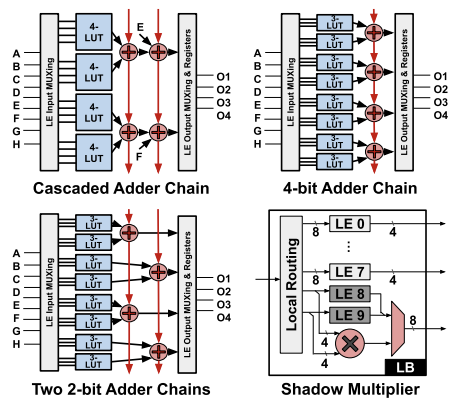
\includegraphics[width=0.75\linewidth]{assets/fpga_13.png}
    \caption{Bốn sửa đổi kiến trúc đối với các phần tử logic (LEs) và khối logic (LBs) của FPGA nhằm tăng mật độ các phép nhân–cộng (MAC) độ chính xác thấp trong logic mềm (soft logic).}
    \label{fig:fpga_13}
\end{figure}
Những ý tưởng này có chi phí diện tích và hiệu suất khác nhau. Ví dụ, đề xuất chuỗi cộng 2-bit cho phép tăng mật độ nhân ma trận lên 1.5 lần và tăng tốc 10\% đồng thời có lợi cho các benchmark không DL, với chi phí tăng diện tích chỉ khoảng 3\% so với kiến trúc cơ sở tương tự Stratix-10. Trong khi đó, thêm shadow multiplier 9-bit vào mỗi LB mang lại mật độ cao hơn 2.4 lần và tốc độ nhanh hơn 17\% nhưng làm tăng diện tích die lên 15\%. Một bằng sáng chế của Intel đã cải tiến đề xuất chuỗi cộng nối tiếp để đạt ánh xạ MAC dày đặc hơn, nhưng phương pháp này hiện chưa được áp dụng rộng rãi trong các kiến trúc FPGA thương mại.

Ngoài ra, các phép toán MAC và popcount trong các mô hình DL độ chính xác thấp hoặc nhị phân thường đòi hỏi phải cộng nhiều hơn 3 bit và có thể được tối ưu bằng cách sử dụng các bộ cộng song song hoặc compressor tổng quát. Một bộ cộng đầy đủ (full adder) nhận 3 bit (A, B, Cin) và nén chúng thành 2 bit (tổng S và carry Cout), thường được gọi là compressor C3:11. Khái niệm này có thể được mở rộng cho bất kỳ số lượng bit đầu vào nào, với đầu ra của compressor đơn giản là số lượng bit 1 trong các đầu vào. Khi phân tích nhiều microbenchmark người ta nhận thấy hơn 35\% các compressor trong các thiết kế này là các compressor C6:111, có thể xem như ba hàm logic 6 đầu vào (một cho mỗi bit đầu ra) ánh xạ thành 3 LE. Một trong số đó là một cổng XOR 6 đầu vào đơn giản. Trong, việc bổ sung một cổng XOR cứng 6 đầu vào vào kiến trúc LE hiện đại (tương tự như Hình \ref{fig:fpga_11}) cho phép một LE hiện thực hai trong số ba hàm logic của compressor C6:111, từ đó đạt được ánh xạ compressor dày đặc hơn tới 36\% với chi phí tăng diện tích dưới 0.5\%.

Kim et al. cũng đề xuất hai cải tiến cho chuỗi cộng cứng trong LB nhằm cải thiện hiệu quả của các phép popcount trong mô hình DL nhị phân. Đề xuất thứ nhất bổ sung một chuỗi cộng popcount mới, lan truyền các bit tổng qua kết nối chuyên dụng và tạo ra các bit carry đầu ra cho các LE (khác với chuỗi cộng truyền thống chỉ lan truyền bit carry). Đề xuất thứ hai bổ sung một bộ cộng đầy đủ khác để cộng hai bit carry đầu ra của hai chuỗi popcount trong một LE. Hai cải tiến này giúp giảm mức sử dụng logic của các phép popcount với các độ rộng khác nhau từ 23\% đến 44\% và từ 36\% đến 40\%, với chi phí tăng diện tích LB chỉ từ 1.9\% đến 2.4\%.
 
\subsubsection{Khối DSP}
Cùng hướng tăng cường hiệu quả các phép MAC độ chính xác thấp trên FPGA, các nghiên cứu học thuật và các nhà cung cấp FPGA đã điều tra thêm hỗ trợ gốc cho các độ chính xác thấp trong các khối DSP truyền thống. Như đã đề cập ở phần III-B, các ứng dụng truyền thông không dây và lọc tín hiệu là động lực chính cho thiết kế các khối DSP. Do đó, cho đến quy trình 14nm, các khối DSP trong FPGA thương mại của Intel (Stratix 10) và AMD (Ultrascale+) đều hỗ trợ các độ chính xác số phù hợp cho các ứng dụng truyền thông. Vào năm 2013, Intel đã bổ sung hỗ trợ số thực đơn (fp32) gốc vào khối DSP của các thiết bị Arria 10 (và sau này là Stratix 10) nhằm nâng cao hiệu quả cho tính toán hiệu năng cao. Sự phát triển nhanh chóng của lĩnh vực DL đã thúc đẩy công trình là nghiên cứu đầu tiên 
điều tra các tối ưu hóa vi kiến trúc DSP cho DL độ chính xác thấp.
\begin{figure} [!h]
    \centering
    \includegraphics[width=0.75\linewidth]{assets/fpga_14.png}
    \caption{Các cải tiến đối với các khối DSP của FPGA để phục vụ học sâu}
    \label{fig:fpga_14}
\end{figure}

Công trình này đã cải tiến một khối DSP kiểu Arria-10, vốn có thể hiện thực một phép nhân int27 hoặc hai phép nhân int18, để hỗ trợ gốc bốn phép nhân và tám phép MAC với các độ chính xác int9 và int4 với chi phí diện tích thấp, như được minh họa ở bên trái Hình \ref{fig:fpga_14}. Điều này đạt được bằng cách cân bằng thêm các mảng nhân 4-bit nhỏ và mạch chi phí thấp cho phép phân chia mảng nhân hiện có thành nhiều mảng con độc lập. Hơn nữa, chuỗi giảm và cộng tích lũy được chia thành hai kênh như trong Hình \ref{fig:fpga_14} để giảm thiểu chi phí diện tích và độ trễ cho chế độ MAC đối với các độ chính xác này. Thiết kế khối DSP cải tiến này được định hướng bởi ba nguyên tắc: (1) đảm bảo tương thích ngược để các khối DSP vẫn hiệu quả cho các ứng dụng không DL, (2) tác động tối thiểu đến diện tích và tần số hoạt động của khối DSP, và (3) giữ nguyên số lượng cổng vào/ra của khối DSP để tránh tăng chi phí diện tích của giao diện định tuyến lập trình được và ngăn chặn các “hot spots” định tuyến xung quanh khối DSP.

Khối DSP cải tiến từ đã tăng diện tích khối DSP thêm 12\%, tương ứng chỉ tăng 0.6\% diện tích die tổng thể của các thiết bị giàu DSP, mà không ảnh hưởng đến tần số hoạt động. Khi được sử dụng trong một số thiết kế bộ tăng tốc DL, các khối DSP mới đã nâng cao hiệu suất lên 1.3× và 1.6× đồng thời giảm mức sử dụng tài nguyên xuống 15\% và 30\% cho các độ chính xác int9 và int4, tương ứng. Sau đó, các kiến trúc FPGA thương mại của Intel (Agilex) và Xilinx (Versal) cũng bổ sung hỗ trợ gốc tương tự cho bốn và ba phép nhân int8/int9 trên mỗi khối DSP, tương ứng.

Các khối DSP truyền thống cũng có các dây nối chuyên dụng cho phép truyền đầu vào/đầu ra từ khối này sang khối DSP kế tiếp trong cùng một cột, ban đầu được thiết kế để hỗ trợ các mảng systolic 1 chiều cho bộ lọc FIR trong các ứng dụng truyền thông không dây. Tuy nhiên, đối với DL, các phép nhân ma trận và tích chập có thể được hiện thực dưới dạng mảng systolic 2 chiều. Do đó, Rasoulinezhad et al. đã đề xuất thêm một mẫu kết nối chuyên dụng giữa các khối DSP để ánh xạ các mảng systolic 2D lên một cột khối DSP mà không cần sử dụng định tuyến lập trình được, như minh họa bên phải Hình \ref{fig:fpga_14}. Họ cũng đề xuất tích hợp một bộ nhớ nhỏ (file thanh ghi hoặc FIFO) bên trong khối DSP nhằm tăng hiệu quả năng lượng bằng cách lưu trữ dữ liệu rất gần với các đơn vị tính toán, cho phép tái sử dụng các toán hạng qua nhiều phép tính mà không cần truy cập từ bộ nhớ LUT hoặc BRAM phân tán. Khối DSP PIR do họ đề xuất đã giảm tiêu thụ năng lượng trung bình xuống 70\%, 82\% và 87\% cho các độ chính xác int9, int4 và int2 so với khối DSP kiểu Xilinx, với chi phí tăng diện tích khối DSP thêm 28\%.

\subsubsection{BRAMs}
Trong các ứng dụng DL, BRAM của FPGA được sử dụng như bộ nhớ tạm do người dùng quản lý để lưu trữ các toán hạng (trọng số và kích hoạt) và kết quả, cung cấp dữ liệu cho các đơn vị tính toán với băng thông rất cao nhờ tính phân tán của chúng. Tuy nhiên, sự tách biệt giữa các đơn vị tính toán (được hiện thực qua LB và DSP) và bộ nhớ (BRAM) đòi hỏi phải di chuyển dữ liệu giữa chúng, làm tăng tải lên hệ thống định tuyến lập trình được, gây ra các “hot spots” định tuyến và tăng tiêu thụ điện năng.

Để giải quyết những thách thức này, nhiều nỗ lực nghiên cứu đã đề xuất thêm khả năng tính toán trực tiếp vào BRAM bằng cách tích hợp các phần tử xử lý (PE) nhẹ ở mức bit ngay bên trong BRAM, từ đó đưa tính toán gần dữ liệu nhất có thể. Điều này mang lại ba lợi ích chính:
\begin{enumerate}
    \item Tăng thông lượng tính toán của FPGA vì một phần lớn diện tích die có thể được sử dụng cho tính toán.
    \item Giảm chuyển động dữ liệu, tiết kiệm năng lượng và tài nguyên định tuyến quý giá.
    \item Cung cấp tính song song tính toán khổng lồ khi số lượng các bitline của BRAM hoạt động như các lane SIMD xử lý theo kiểu bit-serial trên toàn bộ các bit của một từ bộ nhớ.
\end{enumerate}

Để kích hoạt tính toán trong BRAM, cần thêm các PE thực hiện các phép tính bit-serial trên đầu ra của các bộ khuếch đại (sense amplifiers) bên trong BRAM. Cụ thể, hai hàng N-bit (wordlines) được đọc đồng thời từ mảng cell SRAM, các PE thực hiện các phép toán nhị phân song song giữa các bit tương ứng của hai hàng, sau đó kết quả được ghi trở lại một hàng khác trong mảng. Toàn bộ quá trình read-modify-write này diễn ra hoàn toàn bên trong BRAM trong một chu kỳ đồng hồ, chu kỳ này thường dài hơn chu kỳ đọc/ghi thông thường. Bên cạnh các PE của sense amplifiers, cần có mạch điều khiển nhẹ (máy trạng thái hữu hạn) để điều phối các bước này. Các hàng cần đọc, phép tính cần thực hiện và hàng cần ghi tạo thành một lệnh tính toán được cung cấp cho BRAM thông qua các cổng định tuyến lập trình sẵn.

\begin{figure} [!h]
    \centering
    \includegraphics[width=0.75\linewidth]{assets/fpga_15.png}
    \caption{Kiến trúc bên trong của bộ nhớ BRAM trên FPGA, với các thành phần được thay đổi hoặc thêm vào để hỗ trợ tính toán trong bộ nhớ (in-memory compute)}.
    \label{fig:fpga_15}
\end{figure}

Hình \ref{fig:fpga_15} minh họa sơ đồ cấp cao của một BRAM FPGA với các thành phần thay đổi hoặc được bổ sung để tích hợp tính toán trong bộ nhớ (được đánh dấu màu đỏ). Mảng cell SRAM hai cổng ở lõi BRAM không thay đổi. Trong BRAM thông thường, bộ giải mã cột kích hoạt một tập con các bit trong một hàng để các bộ khuếch đại đọc hoặc driver ghi hoạt động. Ví dụ, một mảng SRAM 20Kb (tương tự như trong các BRAM của FPGA Intel hiện đại) được sắp xếp thành 128 hàng, mỗi hàng 160 bit. Tuy nhiên, chiều rộng đọc/ghi tối đa của BRAM là 40 bit nhằm hạn chế chi phí giao diện định tuyến lập trình. Do đó, khối BRAM bao gồm 40 bộ khuếch đại và 40 driver ghi, với bộ giải mã cột chọn một phần 40-bit của hàng 160-bit đó. Để tối đa hóa tính song song cho tính toán trong BRAM, các bộ khuếch đại và driver ghi bổ sung cũng như các PE mức bit được thêm vào để đọc, tính toán và ghi toàn bộ chiều rộng của hàng mảng. Mạch điều khiển cũng được sửa đổi để hỗ trợ quá trình đọc, tính toán và ghi trong một chu kỳ (chu kỳ này dài hơn). Một chân giao diện bổ sung được thêm vào BRAM; khi chân này được kích hoạt, dữ liệu và địa chỉ vào được coi là một lệnh tính toán trong bộ nhớ (CIM). Trong chế độ CIM, mạch glue logic của CIM sẽ giải mã lệnh thành các tín hiệu điều khiển mức thấp cho các thành phần nội bộ của BRAM.

\begin{figure}
    \centering
    \includegraphics[width=0.75\linewidth]{assets/fpga_16.png}
    \caption{Mạch phần tử xử lý tính toán trong bộ nhớ (Compute-in-memory) dành cho phép cộng theo từng bit (bit-serial addition).
(b) Ví dụ về phép tính trong BRAM cho phép cộng từng phần tử giữa hai vectơ có N phần tử, với toán hạng 4-bit.}
    \label{fig:fpga_16}
\end{figure}

Hình \ref{fig:fpga_16}a minh họa sơ đồ một PE tính toán trong bộ nhớ (CIM PE) có khả năng thực hiện phép cộng theo kiểu bit-serial. Trên đường đọc, các bit toán hạng A và B được đọc từ hai hàng của mảng cell SRAM thông qua các sense amplifiers của hai cổng. Hai cổng XOR (SGEN) tạo ra bit tổng (Sum) dựa trên A, B và carry từ chu kỳ trước (Cin). Một bộ cổng khác (CGEN) tính toán bit carry, được lưu vào flip-flop carry (C) cho chu kỳ kế tiếp. Các đầu ra A và B cũng được chuyển đến các cổng Dout theo đường đọc thông thường. Trên đường ghi, các bộ MUX 2 đầu vào (Ws) được thêm vào trước driver ghi (WD) cho hai cổng, lựa chọn giữa bit tổng/carry và dữ liệu thông thường (Din) dựa trên tín hiệu điều khiển từ mạch glue logic CIM.

Hình \ref{fig:fpga_16}b minh họa một ví dụ về hoạt động tính toán trong BRAM để thực hiện phép cộng phần tử của hai vector gồm N phần tử (toán hạng 1 và 2), trong đó mỗi phần tử là số nguyên 4-bit. Các phần tử vector được lưu theo bố cục chuyển vị, sao cho mỗi phần tử của vector đầu tiên được lưu ở một cột khác nhau qua 4 hàng (i đến i+3) và các phần tử của vector thứ hai được lưu ở cùng các cột qua 4 hàng khác (j đến j+3). Trong một chu kỳ, hàng i và j được đọc từ hai cổng của mảng SRAM hai cổng, mỗi PE nhận được một bit từ mỗi hàng và tính tổng của hai bit đó cùng với carry từ chu kỳ trước. Carry-out được lưu vào flip-flop của PE, và tổng được ghi vào hàng k bằng một cổng. Quá trình này lặp lại trong 4 chu kỳ với việc tăng địa chỉ hàng, và trong chu kỳ thứ 5, các bit carry cuối cùng được ghi vào hàng k+4 bằng cổng ghi thứ hai, từ đó kết quả cuối cùng của phép cộng phần tử được lưu ở các hàng từ k đến k+4. Các phép toán phức tạp hơn (như nhân hay phép rút gọn) có thể được hiện thực thông qua chuỗi các phép cộng và sao chép dữ liệu.

Có nhiều đề xuất học thuật nhằm tăng cường khả năng tính toán trong BRAM; các đề xuất này lựa chọn các mô hình tính toán khác nhau (bit-serial so với bit-parallel), các phép toán được hỗ trợ trong các PE bổ sung, cách lưu trữ dữ liệu và kết quả trung gian, cũng như cách lập trình/điều khiển BRAM để thực hiện chuỗi các phép toán. 

Ví dụ, công trình của Wang et al. là nghiên cứu đầu tiên đề xuất thêm khả năng tính toán tương tự như đã được minh họa cho cache của CPU vào BRAM FPGA. Compute-capable BRAM (CCB) của họ sử dụng PE cộng bit-serial; tuy nhiên, nó chỉ sử dụng một cổng bằng cách kích hoạt đồng thời hai wordline để thực hiện một phép AND analog trên các bitline. Phương pháp này giúp giảm chi phí PE và giải phóng một cổng của BRAM, cho phép chồng dữ liệu và tính toán. Tuy nhiên, kỹ thuật này kém ổn định hơn, nhạy cảm với biến thiên quy trình và yêu cầu hạ điện áp wordline (và do đó tần số hoạt động thấp hơn) để tránh làm hỏng nội dung của cell. Một bộ tăng tốc DL thiết kế cho CCB đạt được hiệu suất cao hơn 1.25× và 3× so với bộ tăng tốc Microsoft Brainwave cho độ chính xác int8 và bfp8 trên các tải công việc RNN, GRU và LSTM, với chi phí tăng diện tích die FPGA chỉ 1.8\%. Tương tự, Compute RAM thực hiện các phép AND analog trên các bitline và sử dụng PE cộng bit-serial, nhưng bổ sung thêm một mảng bộ nhớ phụ nhỏ để lưu trữ lệnh bên trong khối BRAM.

Kiến trúc CoMeFa cải thiện độ ổn định so với CCB bằng cách tránh sử dụng phép AND analog trên các bitline; thay vào đó, nó tận dụng tính chất hai cổng của BRAM để lấy hai toán hạng và sử dụng PE cộng bit-serial như Hình \ref{fig:fpga_16}a. Kỹ thuật này đạt tốc độ cao hơn nhưng sử dụng cả hai cổng của BRAM, do đó không thể chồng dữ liệu và tính toán. CoMeFa có các biến thể tối ưu về diện tích và độ trễ; phiên bản tối ưu độ trễ tăng diện tích die FPGA 3.8\% và đạt cải thiện hiệu suất 2.5× trên nhiều tải DL trên một kiến trúc tương tự Brainwave. Cả CCB và CoMeFa đều theo mô hình tính toán bit-serial với dữ liệu được lưu theo bố cục chuyển vị. Trong các ứng dụng DL, một tập hợp toán hạng (trọng số mô hình) là cố định và có thể chuyển vị ngoại tuyến, nhưng chỉ ra rằng việc hiện thực một đơn vị chuyển vị để chuyển đổi tập hợp còn lại (kích hoạt) trong thời gian chạy tiêu tốn nhiều tài nguyên logic mềm. Chen et al. đề xuất kiến trúc tính toán trong BRAM cho phép thực hiện phép nhân-tích lũy (BRAMAC) sử dụng kết hợp tính toán bit-serial và bit-parallel để giảm độ trễ và hỗ trợ các giá trị kích hoạt không chuyển vị. Các PE trong BRAMAC là các bộ cộng có độ chính xác biến đổi, có thể lấy đầu vào từ các nhóm bitline để thực hiện cộng theo kiểu bit-parallel; phép nhân được hiện thực bằng cách cộng dồn kết quả theo kiểu bit-serial. Phương pháp này giảm đáng kể độ trễ tính toán so với cách tiếp cận thuần bit-serial, từ O($m^2$) xuống O($m$) chu kỳ đối với các toán hạng m-bit. Tuy nhiên, nó giới hạn các độ chính xác số mà kiến trúc hỗ trợ vào một tập hợp định sẵn, trong khi cách tiếp cận bit-serial có thể hiện thực bất kỳ độ chính xác nào. BRAMAC còn bổ sung một mảng SRAM phụ nhỏ với vài wordline bên trong khối BRAM. Trong chế độ tính toán, các toán hạng được sao chép nội bộ (hai từ 40-bit mỗi chu kỳ) vào mảng phụ, nơi thực hiện các phép tính, giúp tăng tần số chế độ tính toán do các bitline ngắn hơn, đồng thời cho phép cả hai cổng của mảng chính được sử dụng cho các hoạt động đọc/ghi thông thường trong khi tính toán diễn ra trên mảng phụ. Các biến thể của kiến trúc BRAMAC cho thấy cải thiện hiệu suất từ 1.3× đến 2× cho các mô hình CNN chạy trên bộ tăng tốc tương tự Intel DLA với chi phí tăng diện tích die từ 3.4\% đến 6.8\%. M4BRAMbổ sung PE của BRAMAC bằng cách thêm logic nhân bản và xáo trộn nhằm tăng cường tái sử dụng dữ liệu và hỗ trợ các phép toán hỗn hợp (trọng số và kích hoạt có bề rộng bit khác nhau). Những cải tiến này nâng cao hiệu suất trung bình 1.4× so với BRAMAC.

\subsection{Khối tensor nội mạch (IN-FABRIC TENSOR BLOCKS)}
\begin{figure} [!h]
    \centering
    \includegraphics[width=0.75\linewidth]{assets/fpga_17.png}
    \caption{In-fabric 2D systolic tensor block}
    \label{fig:fpga_17}
\end{figure}
Một hướng nghiên cứu khác là tích hợp các khối cứng mới chuyên dụng cho các phép tính tensor vào mạch FPGA nhằm tăng hiệu quả suy luận DL. Arora et al.đã đề xuất thêm các khối tensor 2D systolic vào mạch FPGA, như minh họa ở Hình \ref{fig:fpga_17} các khối này được bổ sung thêm, chứ không thay thế các khối DSP truyền thống. Các khối tensor này chứa 16 PE, mạch logic vào để chuẩn bị dữ liệu (ví dụ: các thanh ghi trễ để điều chỉnh thời gian đầu vào trong xử lý 2D systolic), mạch logic ra để tập hợp dữ liệu từ các PE và mạch logic định tuyến để cấu hình chế độ hoạt động của khối. Mạch logic định tuyến cho phép khối tensor hoạt động ở chế độ tensor (tất cả các PE cùng tính toán nhân ma trận, nhân ma trận – vector hoặc các phép toán phần tử) hoặc ở chế độ scalar (mỗi PE thực hiện một phép nhân hoặc MAC độc lập). Chế độ hoạt động có thể được thay đổi động theo thời gian bằng cách điều chỉnh các tín hiệu điều khiển. Mỗi PE trong khối tensor có thể hiện thực 1 phép MAC int16, fp16 hoặc bfloat16 16-bit và có thể được “phân tách” để thực hiện 4 phép MAC int8.

Khối tensor này có diện tích gấp 4.4 lần so với một khối DSP kiểu Agilex của Intel, với số cổng vào/ra nhiều hơn gấp 2.4 lần và 4 lần so với khối DSP truyền thống. Để đáp ứng yêu cầu về diện tích và số lượng tín hiệu, các khối này chiếm nhiều vị trí trong lưới định tuyến của FPGA; một khối tensor đơn nằm trên 8 hàng và một cột khối tensor rộng gấp 3.5 lần so với một cột LB. Trên một tập hợp 9 bộ benchmark DL, việc bổ sung các khối tensor nội mạch này đã tăng tần số hoạt động tối đa lên 65\% và giảm chiều dài dây định tuyến trung bình xuống 55\%. Một số phép MAC và kết nối giữa chúng có thể được ánh xạ vào các PE của một khối tensor đơn, đạt được cải thiện về tốc độ và giảm chiều dài dây định tuyến so với việc sử dụng các LB và DSP phân tán. Tuy nhiên, với các bộ benchmark không thuộc DL, các khối tensor không chỉ bị trống mà do tính thô của chúng còn buộc các thành phần khác được đặt xa nhau hơn, dẫn đến giảm tần số từ 0.5\% đến 2.5\% và tăng chiều dài dây định tuyến từ 2\% đến 8\% khi tỷ lệ diện tích die dành cho khối tensor thay đổi từ 5\% đến 30\%.

Khi thị trường tăng tốc DL trên FPGA tiếp tục phát triển, một số nhà cung cấp đã ra mắt các dòng FPGA tối ưu DL tích hợp các dạng khối tensor nội mạch. Các thiết bị này đánh đổi tính tương thích ngược bằng cách thay thế hoàn toàn các khối DSP truyền thống (được thiết kế cho truyền thông không dây) bằng các khối tensor mới, được tối ưu hóa cho các mẫu tính toán và độ chính xác số của tải DL.

\begin{figure} [!h]
    \centering
    \includegraphics[width=0.75\linewidth]{assets/fpga_18.png}
    \caption{Kiến trúc bên trong của khối xử lý học máy (MLPB – Machine Learning Processor Block) trong Achronix Speedster7t.}
    \label{fig:fpga_18}
\end{figure}

Ví dụ, FPGA Achronix Speedster7t tích hợp các khối xử lý DL (MLPBs), kết hợp chặt chẽ BRAM và các đơn vị MAC với giao diện định tuyến nội bộ băng thông cao, như minh họa ở Hình \ref{fig:fpga_18}. Sự kết hợp này giảm số lượng giao diện định tuyến đắt tiền cần thiết để cấp dữ liệu cho các đơn vị tính toán bên trong khối. Dữ liệu trọng số và kích hoạt mới có thể được ghi vào BRAM nội bộ với bộ đệm kép qua các giao diện ngoài hẹp, trong khi một tập hợp khác được tái sử dụng cho nhiều phép tính với các kết nối nội bộ rộng giữa BRAM và đơn vị tính toán.

Một lợi ích khác của sự kết hợp chặt chẽ này là cho phép các MLPB cứng hoạt động ở miền xung cao (lên đến 750MHz) so với mạch mềm, mà không cần sử dụng hệ thống định tuyến lập trình được chi tiết. Các MLPB cũng hỗ trợ tự nhiên nhiều độ chính xác phù hợp cho huấn luyện và suy luận DL như int4/8/16, bfp12/16 và fp16/24. Các thiết bị Speedster7t lớn nhất bao gồm 2.560 MLPB, cung cấp tối đa 61.4 và 122.8 TOPS cho int8/bfp16 và int4/bfp12, tương ứng. Cairncross et al đã chứng minh việc sử dụng MLPB của Speedster7t trong một overlay DL 4 lõi cho các ứng dụng suy luận độ trễ thấp, với tần số lên đến 560MHz, đạt hiệu suất đỉnh 36.4 TOPS cho int8 với mức sử dụng 80-100\% trên nhiều tải GEMV, MLP và RNN với kích thước lô là 4.
\begin{figure} [!h]
    \centering
    \includegraphics[width=0.75\linewidth]{assets/fpga_19.png}
    \label{fig:fpga_19}
\end{figure}

Các khối tensor trí tuệ nhân tạo (AITBs) trong FPGA Intel Stratix 10 NX là một ví dụ thương mại khác về tính toán tensor nội mạch. Mục tiêu của chúng là tích hợp tính toán tensor trong FPGA nhưng với cách tiếp cận khác so với các khối tensor học thuật và MLPB của Achronix. AITBs được thiết kế để thay thế trực tiếp các khối DSP trong Stratix 10 về mặt diện tích silicon và giao diện định tuyến (chỉ khác về nội bộ). Một AITB đơn có đủ diện tích để hiện thực tối đa 30 bộ nhân int8 hoặc 60 bộ nhân int4, nhưng đòi hỏi 480 cổng vào và 480 cổng ra, nhiều hơn rất nhiều so với 96 vào và 72 ra của khối DSP truyền thống. Hầu hết các tải DL chủ yếu dựa vào tích lũy các kết quả của nhiều phép nhân và tái sử dụng đầu vào. Intel giải quyết vấn đề này bằng cách thiết kế ba chế độ AITB khác nhau (xem Hình \ref{fig:fpga_19}) để đạt được mật độ số học cao trong giới hạn 96 vào/72 ra; các chế độ dày đặc hơn hỗ trợ các mẫu tính toán ràng buộc (nhưng hữu ích cho DL).
\begin{figure} [!h]
    \centering
    \includegraphics[width=0.75\linewidth]{assets/fpga_20.png}
    \caption{Ánh xạ các hoạt động tích chập khác nhau trong HPIPE sang các chế độ hoạt động khác nhau của Intel Stratix 10 NX AITB.}
    \label{fig:fpga_20}
\end{figure}
Hình \ref{fig:fpga_20} minh họa cách ánh xạ các phép tích chập khác nhau trong HPIPE lên các chế độ hoạt động của AITB trong FPGA Stratix 10 NX. Ở chế độ scalar, AITB thực hiện các phép nhân độc lập với số lượng kết quả giới hạn bởi giao diện định tuyến chung (chỉ 3 phép MAC int8 độc lập với bộ tích lũy 24-bit, tức 72 đầu ra). Ở chế độ vector, các phép nhân được cộng dồn nội bộ để tạo ra một đầu ra, thích hợp cho các phép dot product; AITB trong chế độ này có thể thực hiện 6 phép nhân int8 theo kiểu dot-6 (2 toán hạng × 6 phần tử × 8 bit = 96 đầu vào). Cuối cùng, chế độ tensor cung cấp mật độ số học cao nhất, nhưng với các ràng buộc chặt về đầu vào/ra; chế độ này thực hiện 3 phép dot product int8 dot-10, mỗi phép có bộ tích lũy riêng và giao tiếp chuyên dụng để giảm kết quả giữa các AITB trong cùng một cột. Để giới hạn số lượng đầu vào ở mức 96, một vector vào được phát sóng tới tất cả 3 đơn vị dot product, trong khi 3 vector vào khác được cấp trực tiếp qua các chuỗi thanh ghi tái sử dụng nội bộ. Mặc dù các đầu vào có thể được tái sử dụng trong một thời gian nhất định trong các tính toán DL (ví dụ: tạo ra nhiều bản đồ đặc trưng trong CNN từ cùng một bản đồ đầu vào), chúng vẫn cần được nạp lại để xử lý tập hợp tiếp theo. Điều này đòi hỏi AITB phải hoặc tạm dừng tính toán để nạp các thanh ghi tái sử dụng, hoặc sử dụng khối đầu tiên trong chuỗi các AITB để nạp dữ liệu một cách tuần tự qua giao diện nối giữa các AITB trong khi chuỗi còn lại tiếp tục tính toán.

Các AITB cũng bổ sung mạch logic nhẹ nhằm tái sử dụng các bộ nhân int8 và int4 để hỗ trợ gốc tự động cho bfp16 và bfp12, tương ứng. Như đã thảo luận ở Sec. II-D3, cả bộ tăng tốc HPIPE và NPU đều được tái kiến trúc để tối ưu sử dụng AITB trong FPGA Stratix 10 NX. Ở HPIPE, cả 3 chế độ của AITB được sử dụng cho các phép toán CNN khác nhau như minh họa ở Hình \ref{fig:fpga_20}. Việc xây dựng một mạng lưới định tuyến trong mạch mềm để gom các kích hoạt có trọng số khác 0 phù hợp với chế độ vector của AITB đã giúp HPIPE tăng tốc suy luận tổng thể 1.9× so với sử dụng các khối DSP truyền thống. Trong các phép tích chập dày đặc và pointwise, HPIPE khai thác mật độ số học cao của chế độ tensor bằng cách nạp sẵn kích hoạt vào các chuỗi thanh ghi tái sử dụng và phát sóng trọng số đến tất cả 3 đơn vị dot product trong AITB. Tuy nhiên, chế độ scalar vẫn cần thiết để hiện thực các phép tích chập depthwise do không có khả năng giảm hay tái sử dụng dữ liệu theo chiều kênh đầu vào. Việc kết hợp chế độ tensor và scalar đã giúp HPIPE tăng tốc suy luận CNN dày đặc 5× so với sử dụng các khối DSP truyền thống. Đối với NPU, việc khai thác chế độ tensor của AITB yêu cầu tăng kích thước lô từ 1 lên 3; các kích hoạt từ 3 đầu vào được nạp sẵn vào các chuỗi thanh ghi tái sử dụng trong khi trọng số được phát sóng đến 3 đơn vị dot product, dẫn đến thông lượng cao hơn 3.5× so với NPU sử dụng khối DSP.

Những cải tiến này không làm tăng diện tích die FPGA vì các AITB có cùng diện tích và giao diện định tuyến lập trình như các khối DSP truyền thống. Tuy nhiên, dù hiệu suất cải thiện đáng kể, các AITB vẫn chưa đạt được mức tăng 15× TOPS int8 đỉnh so với các khối DSP nếu không có sự phù hợp tuyệt đối giữa mẫu tính toán và chế độ tensor của AITB, số lượng các vector đầu vào phải là bội số của 10 để vừa khít với các đơn vị dot product, và không có chi phí bổ sung cho việc nạp dữ liệu vào các chuỗi tái sử dụng. Ngoài ra, việc sử dụng hiệu quả AITB đòi hỏi phải tái cấu trúc đáng kể thiết kế ban đầu nhằm phù hợp với các mẫu tính toán được hỗ trợ bởi AITB, do đó các thiết kế tối ưu này trở nên kém di động giữa các dòng FPGA khác nhau.

Trong tương lai, các khối DSP trong dòng FPGA Intel Agilex 5 sẽ hỗ trợ các chế độ từ khối DSP truyền thống (6×int9, 2×int18, 1×int27) cũng như một biến thể của chế độ tensor AITB với chỉ 2 phép dot-10 int8 trên mỗi khối. Cả NPU và HPIPE đều cần không chỉ nhiều phép MAC độ chính xác thấp mà còn một số phép MAC độ chính xác cao, do đó họ sẽ hưởng lợi từ khả năng thực hiện cả hai trong một khối. Những khối lai này được nhắm tới các ứng dụng DL biên, trong đó FPGA hiện thực một hệ thống đầy đủ với các chức năng xử lý tín hiệu khác.




\subsection{Vượt ra khỏi FPGA}
Các phần V và VI đã mô tả các cải tiến hướng DL cho các thành phần mạch FPGA truyền thống cũng như tích hợp các khối tính toán tensor nội mạch. Bên cạnh đó, còn có một số cải tiến kiến trúc nhằm tăng hiệu suất đỉnh thông qua việc tích hợp các bộ tăng tốc dạng coarse-grained, dù là trên cùng một die đơn thể hay trong cùng một gói thông qua công nghệ tích hợp chip tiên tiến.

\subsubsection{Thiết bị Tăng tốc Có khả năng Tái cấu hình (RADs)}
Gần đây, một loại thiết bị tăng tốc có khả năng tái cấu hình (RADs) đã xuất hiện, kết hợp tính tái cấu hình của mạch FPGA với hiệu quả của các bộ tăng tốc ứng dụng dạng coarse-grained và sự linh hoạt của các lõi xử lý tổng quát. Tất cả các thành phần này được kết nối qua mạng lưới trên chip chuyển gói hiệu năng cao (NoC) cho giao tiếp toàn hệ thống.

\begin{figure} [!h]
    \centering
    \includegraphics[width=1\linewidth]{assets/fpga_21.png}
    \caption{Kiến trúc AMD Versal kết hợp mạch FPGA}
    \label{fig:fpga_21}
\end{figure}

Một ví dụ điển hình của RAD là kiến trúc AMD Versal, tích hợp chặt chẽ một lớp FPGA có thể lập trình được, các lõi xử lý Arm Cortex tổng quát và một mảng bộ xử lý vector chuyên dụng gọi là Adaptive Intelligent Engines (AIEs) trên cùng một die 7nm. Các thành phần này, cũng như các module trên mạch FPGA, giao tiếp qua NoC chuyển gói cứng, là kênh duy nhất để truy cập bộ nhớ ngoài (ví dụ: DDR hoặc HBM). Topology của Versal NoC được điều chỉnh sao cho các cột được nhóm lại với nhau và các hàng được nén ở đầu và cuối thiết bị, như minh họa ở Hình \ref{fig:fpga_21}. Topology này phù hợp với cấu trúc theo cột của FPGA, đơn giản hóa bố cục chip và cung cấp băng thông giao tiếp ngang cao tại các vị trí chứa IO tốc độ cao, bộ điều khiển bộ nhớ và mảng AIE. Sự hiện diện của NoC cứng giúp tăng năng suất thiết kế và hỗ trợ hoàn thiện thời gian, loại bỏ nhu cầu tối ưu hóa nhiều vòng lặp cho giao tiếp hệ thống qua định tuyến lập trình được kém hiệu quả. Các module được hiện thực trên mạch FPGA, giao tiếp qua các giao diện không nhạy với độ trễ, có thể được tối ưu hóa độc lập và sau đó kết nối với cổng NoC để giao tiếp với các module khác, các bộ tăng tốc coarse-grained (ví dụ: AIE) và giao diện ngoài.

Ngoài ra, AIE của Versal cải thiện đáng kể khả năng tính toán của kiến trúc bằng cách kết hợp mảng các bộ xử lý vector với định tuyến không gian giống FPGA và trạng thái phân tán, tạo nên một mô hình tính toán lai. Mỗi ô AIE chứa một bộ xử lý vector VLIW chạy ở 1 GHz có thể thực hiện đồng thời 7 phép toán (2 tải vector, 1 lưu vector, 1 phép toán vector và 2 phép toán scalar). Đơn vị vector số nguyên của mỗi ô AIE có thể thực hiện 128 phép MAC int8 mỗi chu kỳ, đạt hiệu suất đỉnh 256 GOPS. Bộ xử lý vector được kết hợp chặt chẽ với 32KB bộ nhớ SRAM địa phương và cơ chế truy cập bộ nhớ trực tiếp (DMA) cho giao tiếp dữ liệu không liền kề. Như minh họa ở Hình \ref{fig:fpga_21}, các ô AIE được sắp xếp thành lưới 2 chiều với mạng liên kết AXI-Stream, có thể thực hiện giao tiếp theo cả chế độ chuyển mạch mạch và chuyển mạch gói giữa các ô. Ngoài ra, còn có kết nối chuyên dụng nối các bộ tích lũy giữa các ô AIE theo dạng sóng rắn; mỗi ô AIE cũng có khả năng trực tiếp đọc/ghi bộ nhớ địa phương của 3 ô lân cận (theo hướng bắc, nam và một hướng phía đông hoặc tây tùy theo bố trí). Thiết bị Versal lớn nhất có mảng 400 ô AIE, cung cấp hơn 100 TOPS tính toán int8, bên cạnh các đơn vị tính toán được hiện thực trên mạch FPGA truyền thống.

\subsubsection{Chiplet DL}
Hầu hết các FPGA hiện đại của AMD và Intel đã sử dụng công nghệ interposer để tích hợp nhiều die FPGA hoặc kết hợp một die FPGA với một hoặc nhiều chiplet giao tiếp I/O trong cùng một gói với mật độ kết nối cao, như minh họa ở hình \ref{fig:fpga_8}. Interposer cũng có thể được sử dụng để xây dựng các thiết bị FPGA hướng đến một miền ứng dụng cụ thể bằng cách tích hợp một chip ASIC chuyên dụng vào cùng một gói, như minh họa ở bên trái Hình \ref{fig:fpga_23}. Công trình của Intel Labs đã đề xuất tích hợp các chiplet tăng tốc khác nhau vào gói FPGA Stratix 10 nhằm tăng hiệu quả suy luận DL cho các tải công việc khác nhau. Trong trường hợp đó, chiplet thực hiện các phép tính tensor chung cho nhiều tải DL, giúp giải phóng tài nguyên mạch FPGA để hiện thực các lớp mô hình thay đổi theo thời gian hoặc các thành phần hệ thống khác như giai đoạn tiền xử lý/hậu xử lý.
\begin{figure} [!h]
    \centering
    \includegraphics[width=0.75\linewidth]{assets/fpga_23.png}
    \caption{Bộ xen kẽ thụ động để tích hợp một cấu trúc FPGA với
chiplet tăng tốc (trái) và RAD xếp chồng 3D (phải).}
    \label{fig:fpga_23}
\end{figure}

Các tiến bộ gần đây trong công nghệ tích hợp chip đã cho phép xếp chồng nhiều die hoạt động lên nhau. Ví dụ, họ hàng GPU Instinct MI300 của AMD được công bố sử dụng công nghệ xếp chồng die hoạt động để tích hợp 13 chiplet, bao gồm lõi CPU và GPU trên cùng với các die xử lý IO và giao thông bộ nhớ. Điều này mở ra vô số khả năng cho các RAD 3D tích hợp mạch FPGA trên một die ASIC nền, hiện thực các bộ nhớ on-chip lớn hơn, các bộ tăng tốc DL chuyên dụng và NoC cấp hệ thống, như minh họa ở Hình \ref{fig:fpga_23}.

\subsection{Kết luận và Hướng đi Tương lai}

Trong bài báo này, chúng tôi đã tổng hợp các đề xuất từ cả học thuật và công nghiệp nhằm nâng cao kiến trúc FPGA cho DL, tận dụng các cơ hội tối ưu hóa ở các thành phần như logic lập trình được, khối DSP, bộ nhớ on-chip, interposers và mạng lưới trên chip. Những cải tiến này hứa hẹn không chỉ mang lại hiệu suất suy luận DL vượt trội mà còn mở ra các hướng đi mới trong thiết kế các thiết bị tăng tốc DL có tính tái cấu hình với hiệu quả cao về chi phí và năng lượng.

Trước khi trình bày chi tiết các đề xuất cụ thể, chúng tôi sẽ giải thích phương pháp định lượng thường được sử dụng để khám phá và đánh giá các kiến trúc FPGA mới, bao gồm việc sử dụng các bộ benchmark và quy trình CAD có khả năng tái định hướng. Các phương pháp này cung cấp cơ sở vững chắc để đo lường tác động của các cải tiến về hiệu suất, diện tích và tiêu thụ năng lượng, từ đó hỗ trợ quyết định thiết kế cho tương lai của FPGA trong các ứng dụng DL.


\subsubsection{So sánh FPGA và ASIC}
FPGA thường linh hoạt và tiết kiệm chi phí hơn so với ASIC. Trong các phần sau, tôi sẽ giải thích lý do tại sao điều này đúng.

Chi phí và tính linh hoạt
Khi sử dụng FPGA, bạn có thể triển khai bất kỳ chức năng logic nào mà một ASIC thực hiện, nhưng với ưu điểm nổi bật là khả năng cập nhật chức năng sau khi chip được sản xuất, điều này rất mong muốn đối với nhiều ứng dụng. FPGA tiết kiệm chi phí hơn ASIC vì khách hàng có thể lập trình FPGA theo yêu cầu của mình thay vì phải thuê một nhà cung cấp để thiết kế và chế tạo một ASIC đáp ứng nhu cầu của họ.

Giảm rủi ro thời gian thiết kế so với tốc độ
Nếu bạn quyết tâm sử dụng quy trình bán dẫn tiên tiến nhất trên thế giới bất chấp chi phí, bạn luôn có thể thiết kế một ASIC chạy nhanh hơn FPGA nhanh nhất hiện có. Tuy nhiên, hầu như không ai sử dụng quy trình tiên tiến nhất: làm như vậy sẽ rất rủi ro, cực kỳ khó khăn và tốn kém đến mức không tưởng. Trên thực tế, chỉ có một số ít công ty sản xuất ASSP (Application-Specific Standard Product) nhảy vào sử dụng quy trình mới ngay khi nó có sẵn. Còn lại, mọi người sử dụng các quy trình đã cũ hơn một, hai hoặc ba thế hệ. Và thực tế là FPGA nhanh nhất mà bạn có thể sở hữu có thể cạnh tranh trực tiếp với các quy trình ASIC cũ hơn đó. Hơn nữa, FPGA mang lại công việc thiết kế ít hơn và rủi ro thấp hơn rất nhiều.

Ví dụ, nếu bạn đang thiết kế một hệ thống với yêu cầu cụ thể về hiệu suất năng lượng và hiệu năng, và dự định sử dụng một ASIC 65 nanomet (nm) cũ hơn, bạn có biết rằng bạn có thể đạt được kết quả tương tự với một FPGA 20 nm hiện tại không? Việc sử dụng FPGA sẽ rút ngắn thời gian thiết kế của bạn, giảm nguy cơ lỗi thiết kế, và cung cấp tổng chi phí sở hữu (TCO) thấp hơn so với ASIC. Đối với hầu hết các ứng dụng, mức tiêu thụ năng lượng của FPGA sẽ ở mức chấp nhận được cho nhu cầu của bạn. Do đó, nhờ vào TCO thấp hơn và tính linh hoạt cao hơn, FPGA thường là lựa chọn công nghệ tốt nhất.

Việc chọn một FPGA cho một hệ thống mang lại cho nhà thiết kế khả năng cấu hình cao hơn cũng như giảm rủi ro ảnh hưởng đến lịch trình phát triển, bởi vì, như được minh họa bởi phép so sánh với LEGO, các phần nhỏ của FPGA có thể được sửa đổi mà không ảnh hưởng đến phần còn lại của thiết kế.

\section{GPU và CPU}

\subsection{GPU vs. CPU: Điểm khác biệt chính}

CPU rất phù hợp cho các tác vụ đòi hỏi xử lý tuần tự. Ngược lại, GPU vượt trội trong các tác vụ như kết xuất và xử lý mô hình AI do khả năng xử lý song song vượt trội của chúng. Điều này làm cho GPU trở nên lý tưởng để hoàn thành các tác vụ phức tạp với hiệu quả hàng đầu.

Mặc dù CPU có thể có nhiều lõi (thường từ 2 đến 64 lõi, ví dụ như bộ xử lý AMD EPYC hoặc Intel Xeon), nhưng chúng vẫn kém hiệu quả hơn đáng kể khi xử lý song song so với GPU có thể có hàng nghìn lõi hoạt động cùng lúc để hoàn thành các hoạt động trong chớp mắt.
Tóm lại, GPU lý tưởng cho các nhu cầu tính toán phức tạp như học máy, mô hình học sâu, phân tích dữ liệu và các ứng dụng trí tuệ nhân tạo khác. Mặt khác, CPU phù hợp hơn cho các tác vụ tính toán mục đích chung như chạy hệ điều hành, phần mềm năng suất và các ứng dụng yêu cầu logic phức tạp hoặc luồng điều khiển.

\subsubsection{Tại sao CPU không thể hoạt động cho nhu cầu tính toán phức tạp}
CPU và GPU có sự khác biệt về mặt kiến trúc và cả hai đều được thiết kế cho các mục đích chung khác nhau. Các đặc điểm của chúng giúp chúng hoạt động tốt trong các tác vụ tương ứng. Hiện tại, bạn đã biết rằng CPU không được thiết kế cho các hoạt động siêu phức tạp như học máy và học sâu.
\paragraph{Xử lý song song}\leavevmode\\
CPU kém hiệu quả hơn trong xử lý song song, điều này hạn chế khả năng đa nhiệm của chúng đối với các hoạt động tính toán chuyên sâu. Nói một cách đơn giản, trong khi các đơn vị xử lý như CPU có thể xử lý các tác vụ song song, chúng hiệu quả hơn nhiều khi xử lý tuần tự.

Các hoạt động phức tạp như học máy sử dụng nhiều lõi để hiểu tác vụ được giao. Nhu cầu năng lượng tăng lên theo độ phức tạp và kích thước của tập dữ liệu được sử dụng để đào tạo AI.

Đó là lý do tại sao các doanh nghiệp đang chuyển sang dịch vụ đồng định vị AI để đào tạo các mô hình AI với các tập dữ liệu khổng lồ. Bạn có được sức mạnh, tốc độ và khả năng mở rộng để xử lý các dự án AI lớn mà không cần phải liên tục nâng cấp hoặc bảo trì phần cứng.

CPU, được thiết kế cho các tác vụ mục đích chung, có băng thông thấp hơn đáng kể so với GPU, được tối ưu hóa để xử lý lượng dữ liệu lớn. Băng thông bộ nhớ cao giúp GPU có thể thực hiện các tác vụ phức tạp như kết xuất hình ảnh 3D hoặc xử lý các tập dữ liệu lớn.

Đó chính xác là những gì học sâu yêu cầu: xử lý hàng tấn dữ liệu cùng lúc, giống như não người hoặc mạng nơ-ron.

\paragraph{Hạn chế về năng lượng}\leavevmode\\

CPU được thiết kế cho các tác vụ nhẹ, tuần tự. Mặc dù chúng cung cấp hiệu quả năng lượng cho các hoạt động cơ bản, nhưng chúng có xu hướng tiêu thụ nhiều điện năng hơn cho các tác vụ đòi hỏi sức mạnh tính toán cao, chẳng hạn như máy móc và học sâu.

Hơn nữa, băng thông hạn chế và khả năng xử lý song song không đủ của chúng buộc chúng phải làm việc chăm chỉ để thực hiện các tác vụ phức tạp, do đó sử dụng thêm năng lượng để hoàn thành tác vụ.

Trong khi đó, GPU được thiết kế riêng để thực hiện các tác vụ như vậy. Chúng có khả năng thực hiện các tác vụ phức tạp nhanh hơn đáng kể bằng cách sử dụng xử lý song song, tiết kiệm rất nhiều năng lượng mà không ảnh hưởng đến hiệu quả.

Do mức tiêu thụ điện năng lớn như vậy, các doanh nghiệp dựa vào các máy chủ dữ liệu trên toàn thế giới, với cấu hình nguồn được tối ưu hóa cho điện toán AI, để thích ứng với các xu hướng và công nghệ trí tuệ nhân tạo mới nổi trong không gian làm việc của họ. Các trung tâm dữ liệu trang bị cho các doanh nghiệp những thứ cần thiết để lưu trữ máy tính của họ trên các máy chủ từ xa.

\subsubsection{Điều gì làm cho GPU trở nên lý tưởng cho khối lượng công việc AI}

GPU sử dụng các mô-đun xử lý song song để hoạt động. Hãy cùng xem xét cách thức hoạt động của nó bằng một ví dụ đơn giản.

Khi được giao một nhiệm vụ, các đơn vị xử lý như GPU sẽ chia nhiệm vụ đó thành các nhiệm vụ nhỏ hơn và sử dụng khả năng xử lý song song của chúng để phân bổ khối lượng công việc trên hàng nghìn lõi, hoàn thành nhiệm vụ hiệu quả hơn.

Hơn nữa, nhiều GPU có thể được tích hợp vào một nút duy nhất để đạt được điện toán hiệu suất cao (HPC), có thể cực kỳ hữu ích cho các lĩnh vực đòi hỏi sức mạnh xử lý lớn.

HPC cực nhanh. Máy tính thông thườngvới bộ xử lý 3 GHz có thể thực hiện hàng tỷ phép tính mỗi giây. Mặc dù nghe có vẻ cực kỳ nhanh, nhưng nó vẫn chậm hơn đáng kể so với HPC có thể thực hiện hàng nghìn tỷ phép tính mỗi giây.

GPU đòi hỏi sức mạnh đáng kể. Cho dù đó là kết xuất đồ họa chân thực, xử lý các mô hình AI khổng lồ hay xử lý các chi tiết ở cấp độ pixel, chúng đều tiêu thụ rất nhiều năng lượng. Nhưng sức mạnh bổ sung đó có nghĩa là hiệu suất mạnh mẽ. Chúng sử dụng nhiều năng lượng hơn, nhưng chúng hoàn thành công việc nhanh hơn và hiệu quả hơn khi cần thiết nhất.

\subsubsection{Đánh giá CPU và GPU cho AI: Ưu và nhược điểm}
Mặc dù GPU có vẻ là lựa chọn tốt nhất cho AI, nhưng cũng cần phải xem xét nhược điểm của chúng. Trong phần này, chúng tôi sẽ đánh giá CPU so với GPU cho AI và chỉ ra ưu và nhược điểm của từng loại.

\paragraph{CPU}\leavevmode\\

Tốt cho các tác vụ AI cơ bản và một số ứng dụng trí tuệ nhân tạo. Gặp khó khăn với các tác vụ phức tạp như mô hình học sâu và mô hình ngôn ngữ lớn.
Tiết kiệm năng lượng cho những công việc nhỏ.
Dễ dàng tích hợp vào các hệ thống máy tính thông dụng hiện có.
Chậm hơn đối với các tác vụ hiệu suất cao như đào tạo mô hình hoặc ứng dụng AI thời gian thực.Giá cả phải chăng hơn, đặc biệt là đối với các ứng dụng đa năng và nhiệm vụ AI cơ bản.Không yêu cầu hệ thống làm mát tiên tiến.Phù hợp hơn cho việc xử lý các tác vụ đơn giản và tính toán mục đích chung.

\paragraph{GPU}\leavevmode\\
Tuyệt vời cho các tác vụ song song như học sâu và mô hình ngôn ngữ lớn. Phù hợp với các đơn vị xử lý AI nặng.Không hiệu quả bằng CPU về mặt tiêu thụ năng lượng.Ít linh hoạt hơn khi tích hợp vào các thiết lập bộ xử lý đồ họa (GPU) truyền thống.Nhanh hơn nhiều đối với các tác vụ AI, máy học và điện toán hiệu suất cao (HPC).Đắt hơn, đặc biệt đối với các mẫu máy cao cấp cần thiết cho AI.Cần có hệ thống làm mát tiên tiến, đặc biệt là trong các thiết lập có mảng cổng lập trình được (FPGA).Ít hiệu quả hơn đối với các tác vụ đơn giản, nhưng lại vượt trội trong xử lý song song cho khối lượng công việc AI lớn hơn.
%%%%%%%%%%%%%%%%%%%%%%%%%%%%%%
\subsection{Kiến trúc GA102 của GPU}
Khi mở GPU ra, ta tìm thấy một chip hoặc khuôn lớn có tên GAML D9 102, được chế tạo từ 28,3 tỷ bóng bán dẫn.
    
\begin{figure}[H]
    \centering
    \includegraphics[width=0.75\linewidth]{assets/gpu1.png}
    \caption{GPU trong card đồ họa}
    \label{fig:enter-label}
\end{figure}
    
Phần lớn diện tích của chip được chiếm bởi các lõi xử lý (Processing Cores), được tổ chức theo kiến trúc phân cấp. Cụ thể, chip được chia thành 7 cụm xử lý đồ họa (Graphics Processing Clusters - GPC), trong mỗi cụm xử lý có 12 bộ đa xử lý luồng (Streaming Multiprocessors - SM).
    
\begin{figure}[H]
    \centering
    \includegraphics[width=0.75\linewidth]{assets/gpu2.png}
    \caption{GPC trong GPU}
    \label{fig:enter-label}
\end{figure}
    
\begin{figure}
    \centering
    \includegraphics[width=0.75\linewidth]{assets/gpu3.png}
    \caption{SM trong GPC}
    \label{fig:enter-label}
\end{figure}
    
Bên trong mỗi bộ đa xử lý luồng này có 4 Warp và 1 lõi dò tia (Ray Tracing Core). Mỗi Warp có 32 lõi CUDA (lõi tạo bóng) và 1 lõi Tensor. Trên toàn bộ GPU có 10.752 lõi CUDA, 336 lõi Tensor và 84 lõi dò tia. Ba loại lõi này thực hiện tất cả các phép tính của GPU, mỗi loại có một chức năng khác nhau.
    
\begin{figure}[H]
    \centering
    \includegraphics[width=0.75\linewidth]{assets/gpu4.png}
    \caption{WARP và Ray tracing core trong SM}
    \label{fig:enter-label}
\end{figure}
    
\begin{figure}[H]
    \centering
    \includegraphics[width=0.75\linewidth]{assets/gpu5.png}
    \caption{Cuda cores và Tensor cores trong Warp}
    \label{fig:enter-label}
\end{figure}
    
\begin{figure}[H]
    \centering
    \includegraphics[width=0.75\linewidth]{assets/gpu6.png}
    \caption{Các loại cores trong GPU}
    \label{fig:enter-label}
\end{figure}

Lõi CUDA có thể được coi là máy tính nhị phân đơn giản với các nút cộng, nút nhân và một vài nút khác, thường được sử dụng nhiều nhất khi chạy trò chơi điện tử.
    
Lõi Tensor là máy tính nhân và cộng ma trận, được sử dụng để biến đổi hình học, làm việc với mạng nơ-ron và AI.
    
Lõi dò tia là lớn nhất nhưng ít nhất, được dùng để thực hiện các thuật toán dò tia.
    
Các card đồ họa 3080, 3090, 3080 Ti, 3090 Ti đều sử dụng cùng một thiết kế chip GA102 cho GPU của chúng. Chúng có giá khác nhau và được phát hành vào những năm khác nhau.
    
\begin{figure}
    \centering
    \includegraphics[width=0.75\linewidth]{assets/gpu7.png}
    \caption{Các dòng GPU từ mạch GA102}
    \label{fig:enter-label}
\end{figure}
    
\begin{figure}
    \centering
    \includegraphics[width=0.75\linewidth]{assets/gpu8.png}
    \caption{Giá bán có sự chênh lệch giữa các dòng GPU}
    \label{fig:enter-label}
\end{figure}
    
\subsection{Quá trình sản xuất GPU GA102}

Trong quá trình sản xuất, các lỗi tạo mẫu, hạt bụi hoặc sự cố sản xuất khác có thể gây ra hư hỏng và tạo ra các vùng mạch bị lỗi. Thay vì vứt bỏ toàn bộ chip vì một lỗi nhỏ, các kỹ sư xác định vùng bị lỗi, cách ly vĩnh viễn và vô hiệu hóa mạch điện gần đó. Nhờ thiết kế GPU có tính lặp lại cao, một lỗi nhỏ chỉ làm hỏng một bộ đa xử lý luồng cụ thể mà không ảnh hưởng đến các khu vực khác của chip. Kết quả là các chip này được thử nghiệm và phân loại dựa trên số lượng lỗi để theo dõi.
    
\begin{figure}
    \centering
    \includegraphics[width=0.75\linewidth]{gpu9.png}
    \caption{Vô hiệu hóa một vùng mạch}
    \label{fig:enter-label}
\end{figure}
    
Card đồ họa 3090 Ti sử dụng chip GA102 hoàn hảo với tất cả 10.752 lõi CUDA hoạt động bình thường, 3090 có 10.496 lõi hoạt động, 3080 Ti có 10.240 lõi và 3080 có 8.704 lõi hoạt động.
    
\begin{figure}
    \centering
    \includegraphics[width=0.75\linewidth]{assets/gpu10.png}
    \caption{Clock speed trên từng loại GPU}
    \label{fig:enter-label}
\end{figure}
Ngoài ra, các card đồ họa khác nhau còn khác nhau về tốc độ xung nhịp tối đa, số lượng và thế hệ bộ nhớ đồ họa hỗ trợ (GPU).

\subsection{Thiết kế CUDA Cores}
CUDA Core là một đơn vị xử lý trong GPU NVIDIA, được thiết kế để tính toán song song hiệu quả cao. Một GPU có thể có hàng nghìn CUDA Core chia nhỏ khối lượng công việc thành các phần nhỏ hơn và xử lý chúng đồng thời.
Ở cấp độ cao, lõi CUDA hoạt động bằng cách thực hiện các hoạt động SIMT (Lệnh đơn, Nhiều luồng). Điều này có nghĩa là nhiều lõi CUDA thực hiện cùng một lệnh trên các phần dữ liệu khác nhau song song. Kiến trúc này đặc biệt phù hợp với các tác vụ như kết xuất đồ họa, mô phỏng khoa học và các khối lượng công việc tính toán hiệu suất cao khác.
CUDA Core dựa vào tính song song lớn và băng thông bộ nhớ cao để đạt được hiệu suất tăng trong các ứng dụng tính toán chuyên sâu.
Khi một chương trình được viết bằng CUDA (nền tảng điện toán song song của NVIDIA) chạy trên GPU, nó sẽ sắp xếp các tác vụ thành lưới, khối và luồng. Mỗi luồng được gán cho một lõi CUDA và thực hiện đồng thời các phần nhỏ của phép tính. Đó là cách GPU có thể xử lý lượng dữ liệu khổng lồ cùng một lúc.
    
\begin{figure}
    \centering
    \includegraphics[width=0.75\linewidth]{assets/gpu11.png}
    \caption{Thiết kế Cuda core}
    \label{fig:enter-label}
\end{figure}
    
\textbf{Vai trò CUDA cores khi tích hợp trong GPU}
\begin{itemize}
    \item Xử lý song song: CUDA cores giúp GPU xử lý hàng nghìn luồng dữ liệu cùng lúc,
    điều này rất quan trọng trong học sâu (Deep Learning) và xử lý đồ họa.
    \item Tăng hiệu suất: CUDA cores đảm bảo GPU xử lý các tác vụ như thực hiện phép nhân và phép cộng hợp nhất (FMA - Fused Multiply and Add) (A x B + C), kết xuất đồ họa 3D và huấn luyện mô hình AI nhanh chóng hơn so với CPU.
    \item Tối ưu cho AI: Hỗ trợ các thuật toán AI như học sâu và mạng nơ-ron tích chập.
\end{itemize}
\subsection{Tensor Cores}
Lõi tensor là một đơn vị xử lý chuyên dụng trong GPU NVIDIA được thiết kế để tăng tốc các hoạt động tensor, đặc biệt là phép nhân ma trận, vốn là nền tảng cho học sâu và điện toán hiệu suất cao. Trong khi lõi CUDA xử lý khối lượng công việc song song mục đích chung, lõi tensor được tối ưu hóa cho điện toán độ chính xác hỗn hợp, cho phép chúng thực hiện khối lượng lớn các phép tính dấu phẩy động hiệu quả hơn nhiều so với lõi CUDA truyền thống.

Ở cấp độ cao, lõi tensor hoạt động bằng cách thực hiện các phép toán nhân-cộng hợp nhất (FMA) trên ma trận trong một bước duy nhất, thay vì chia chúng thành nhiều lệnh. Về cơ bản, Tensor Cores lấy ba ma trận, nhân hai ma trận đầu tiên, cộng vào ma trận thứ ba, rồi xuất ra kết quả. Vì tất cả các giá trị của ba ma trận đầu vào đã sẵn sàng cùng một lúc, Tensor Cores hoàn thành tất cả các phép tính nhân và cộng ma trận đồng thời. Mạng nơ-ron trong AI tổng quát yêu cầu hàng nghìn tỷ đến hàng triệu tỷ phép toán nhân và cộng ma trận, thường sử dụng các ma trận lớn hơn nhiều.  Điều này làm cho chúng trở nên lý tưởng cho khối lượng công việc học sâu, trong đó mạng nơ-ron đòi hỏi phép nhân và tích lũy ma trận mở rộng.
    
\begin{figure}[H]
    \centering
    \includegraphics[width=0.75\linewidth]{assets/gpu12.png}
    \caption{Cách hoạt động của tensor core}
    \label{fig:enter-label}
\end{figure}
    
Lõi Tensor hỗ trợ các định dạng có độ chính xác thấp hơn như FP16 (half-precision), BF16 (bfloat16) và INT8, đồng thời tận dụng tích lũy FP32 để duy trì độ chính xác. Điều này cho phép lõi Tensor đạt được thông lượng cao hơn nhiều mà không phải hy sinh quá nhiều độ chính xác.
    
\begin{figure}[H]
    \centering
    \includegraphics[width=0.75\linewidth]{assets/gpu13.png}
    \caption{Cách hoạt động của tensor core}
    \label{fig:enter-label}
\end{figure}
    
Lõi Tensor được sử dụng rộng rãi trong AI và các khuôn khổ học sâu như TensorFlow và PyTorch, nơi chúng tăng tốc các phép tính ma trận nặng. Ngoài AI, lõi Tensor còn tăng cường mô phỏng khoa học, HPC workloads và dò tia thời gian thực.

Do cung cấp khả năng tăng cường hiệu suất đáng kể so với lõi CUDA nên lõi tensor đã trở thành yếu tố khác biệt chính trong GPU RTX và trung tâm dữ liệu của NVIDIA.
    
\textbf{Vai trò Tensor Cores khi tích hợp trong GPU}
\begin{itemize}
    \item Tăng tốc học sâu: Tensor cores giúp giảm thời gian huấn luyện các mô hình AI
    lớn, đặc biệt là các mô hình mạng neural sâu (Deep Neural Networks).
    \item Hỗ trợ suy luận AI (Inference): Tensor cores tối ưu hóa tính toán trong các ứng
    dụng yêu cầu dự đoán nhanh, như xử lý ngôn ngữ tự nhiên và nhận diện hình ảnh.
    \item Mixed Precision Training: Tensor cores tận dụng FP16, giảm tài nguyên bộ nhớ
    và cải thiện hiệu năng trong khi duy trì độ chính xác gần FP32.
\end{itemize}

\subsection{CUDA Cores so với Tensor Cores}
    
Lõi CUDA và lõi tensor đều đóng vai trò quan trọng trong tính toán GPU, nhưng chúng được thiết kế cho các loại khối lượng công việc khác nhau. Sau đây là những điểm khác biệt chính:
\begin{itemize}
    \item Mục đích và tối ưu hóa khối lượng công việc \par
    \begin{itemize}
        \item \textbf{Lõi CUDA} là bộ xử lý song song đa năng được thiết kế để xử lý nhiều tác vụ khác nhau, từ kết xuất đồ họa đến các hoạt động tính toán chung. Chúng rất giỏi trong việc song song hóa các khối lượng công việc như rasterization, mô phỏng vật lý và các ứng dụng tính toán nặng truyền thống.
        \item \textbf{Lõi Tensor} là các đơn vị phần cứng chuyên dụng được thiết kế riêng để tăng tốc phép nhân ma trận, là nền tảng của học sâu và AI. Chúng tối ưu hóa khối lượng công việc học sâu bằng cách thực hiện các phép toán Tensor với thông lượng cao hơn nhiều so với lõi CUDA.
    \end{itemize}
    \item Độ chính xác và kiểu dữ liệu\par
    \begin{itemize}
        \item \textbf{Lõi CUDA} chủ yếu hoạt động trên các số dấu phẩy động độ chính xác đơn (FP32) và độ chính xác kép (FP64), điều này khiến chúng phù hợp với nhiều loại tính toán.
        \item \textbf{Lõi Tensor} hỗ trợ phép tính số học độ chính xác hỗn hợp (FP16, BF16, INT8, INT4) với tích lũy FP32, nghĩa là chúng có thể xử lý các phép tính có độ chính xác thấp nhanh hơn nhiều trong khi vẫn duy trì độ chính xác chấp nhận được - điều quan trọng đối với quá trình đào tạo và suy luận học sâu.
    \end{itemize}
    \item Hiệu quả tính toán và tốc độ
    \begin{itemize}
        \item Lõi CUDA thực hiện các hoạt động tuần tự song song, nghĩa là nhiều lõi thực hiện các phép tính đồng thời nhưng ở cấp độ chi tiết hơn.
        \item Lõi Tensor tận dụng các hoạt động nhân-cộng hợp nhất (FMA) để thực hiện nhiều phép tính trong một chu kỳ xung nhịp. Điều này cho phép chúng thực hiện phép nhân ma trận nhanh hơn nhiều lần so với lõi CUDA, đặc biệt là trong khối lượng công việc tính toán khoa học và AI.
    \end{itemize}
    \item Các trường hợp sử dụng\par
    \begin{itemize}
        \item \textbf{Lõi CUDA} được sử dụng cho các tác vụ tính toán song song truyền thống, chẳng hạn như đồ họa chơi game, mô phỏng vật lý, xử lý video và khối lượng công việc GPU thông thường.
        \item \textbf{Lõi Tensor} được tối ưu hóa cho AI, học sâu và điện toán khoa học, nơi các hoạt động ma trận quy mô lớn là rất quan trọng. Chúng tăng tốc đáng kể quá trình đào tạo cho mạng nơ-ron và suy luận cho các mô hình AI.
    \end{itemize}
    \item Có sẵn trong GPU NVIDIA\par
    \begin{itemize}
        \item \textbf{Lõi CUDA} có mặt trong tất cả các GPU NVIDIA, từ card đồ họa tiêu dùng cơ bản đến GPU trung tâm dữ liệu cao cấp.
        \item \textbf{Lõi Tensor} có trong GPU dòng RTX (ví dụ: dòng RTX 30, 40), GPU trung tâm dữ liệu NVIDIA (A100, H100) và GPU cấp máy trạm, nơi khả năng tăng tốc AI được ưu tiên. 
    \end{itemize}
\end{itemize}
\begin{table}[h]
    \centering
    \renewcommand{\arraystretch}{1.3} % Tăng khoảng cách giữa các dòng
    \begin{tabular}{|p{5cm}|p{5cm}|p{5cm}|}
        \hline
        \textbf{} & \textbf{Lõi CUDA} & \textbf{Lõi Tensor} \\
        \hline
        \textbf{Mục đích và tối ưu hóa} & Xử lý song song mục đích chung & Chuyên dùng để tăng tốc phép nhân ma trận \\
        \hline
        \textbf{Độ chính xác} & Chủ yếu là FP32 (độ chính xác đơn) và FP64 (độ chính xác kép) & Hỗ trợ độ chính xác hỗn hợp (FP16, BF16, INT8, INT4) với tích lũy FP32 \\
        \hline
        \textbf{Tốc độ} & Thực hiện các hoạt động tuần tự song song & Các phép toán nhân-cộng hợp nhất (FMA) cho phép tính toán ma trận nhanh hơn đáng kể \\
        \hline
        \textbf{Các trường hợp sử dụng} & Đồ họa chơi game, xử lý video, điện toán GPU mục đích chung & Học sâu, đào tạo/suy luận mô hình AI, mô phỏng khoa học, điện toán hiệu suất cao \\
        \hline
        \textbf{Có sẵn trong GPU NVIDIA} & Có mặt trong tất cả các GPU NVIDIA, từ các mẫu dành cho người tiêu dùng đến các mẫu trung tâm dữ liệu & Được tìm thấy trong dòng RTX, GPU trung tâm dữ liệu (A100, H100) và GPU cấp máy trạm \\
        \hline
    \end{tabular}
    \caption{So sánh lõi CUDA và lõi Tensor trong GPU NVIDIA}
    \label{tab:cuda_tensor_comparison}
\end{table}
\subsection{Các tính năng nổi bật của GPU trong AI}
\begin{itemize}
    \item Tính toán song song: Với hàng nghìn nhân CUDA, GPU có thể thực hiện tính toán song song, lý tưởng cho các phép toán ma trận lớn trong học sâu.
    \item Mixed Precision Training: Sử dụng FP16 (16-bit floating point) thay vì FP32 (32-bit floating point), giúp tăng tốc độ huấn luyện mà vẫn đảm bảo độ chính xác cao.
    \item Tăng tốc độ tính toán: FP16 giảm khối lượng dữ liệu, giúp các nhân xử lý (Tensor Cores) thực hiện phép toán nhanh hơn.
    \begin{itemize}
        \item Tiết kiệm bộ nhớ: Với kích thước nhỏ hơn, FP16 cho phép lưu trữ nhiều thông số mô hình hơn trên GPU.
        \item Hỗ trợ từ phần cứng: Các GPU hiện đại, như NVIDIA Tensor Cores, được tối ưu hóa cho tính toán FP16, giúp tăng hiệu suất tổng thể.
        \item Độ chính xác đảm bảo: Một số kỹ thuật được sử dụng để đảm bảo độ chính xác khi sử dụng FP16, khiến độ chính xác gần tương đương FP32 trong hầu hết các trường hợp.
    \end{itemize}
    \item Tối ưu hóa bộ nhớ: Các GPU hiện đại như NVIDIA A100 hỗ trợ bộ nhớ HBM2e (Băng thông 410Gbps thay vì 128Gbps của HBM) và NVLink để truyền tải dữ liệu nhanh hơn giữa các GPU.
\end{itemize}

\subsection{Ứng dụng của GPU trong AI}
\textbf{Huấn luyện mô hình học sâu (Deep Learning Training):} GPUs được sử dụng rộng rãi
trong huấn luyện các mô hình mạng neural sâu (Deep Neural Networks) do khả năng xử lý
song song và băng thông bộ nhớ cao.

\textbf{Suy luận AI (AI Inference):} GPUs cũng rất hiệu quả trong quá trình suy luận mô hình,
đặc biệt là các mô hình yêu cầu tính toán nhanh như nhận diện hình ảnh, phân loại văn bản,
và xử lý ngôn ngữ tự nhiên.

\textbf{Xử lý hình ảnh và video (Image and Video Processing):} Các mô hình AI xử lý video
độ phân giải cao và ứng dụng thị giác máy tính (computer vision) yêu cầu băng thông lớn và
khả năng tính toán song song.

\subsection{Ví dụ về các dòng GPU AI hiện đại}
\textbf{NVIDIA A100:} Dành cho các trung tâm dữ liệu AI, có khả năng xử lý song song với
6912 nhân CUDA và bộ nhớ HBM2e dung lượng lớn.

\textbf{NVIDIA RTX 3090 và RTX 4090:} Dành cho các máy trạm (workstation) và người dùng
cá nhân, hỗ trợ Tensor Cores, tối ưu cho cả AI và xử lý đồ họa.

\textbf{AMD Radeon Instinct MI200:} Một lựa chọn khác từ AMD cho các trung tâm dữ liệu
AI, với băng thông bộ nhớ cực cao và hiệu năng tính toán vượt trội.

\subsection{Thách thức và hạn chế}
\textbf{Tiêu thụ điện năng:} GPUs tiêu thụ nhiều năng lượng hơn so với CPU, đặc biệt khi được
sử dụng trong các trung tâm dữ liệu lớn.

\textbf{Chi phí cao:} Các GPU AI cao cấp như NVIDIA A100 hoặc RTX 4090 có giá thành rất
cao, điều này có thể là rào cản đối với các công ty nhỏ hoặc nhóm nghiên cứu học thuật.

\textbf{Yêu cầu về phần cứng bổ trợ:} Để tận dụng tối đa sức mạnh của GPU, cần có hệ thống
làm mát tốt và nguồn cấp điện đủ mạnh.
%%%%%%%%%%%%%%%%%%%%%%%%%%%%%%

\section{Thảo luận và kết luận}
\subsection{Vai Trò của AI Chips}
AI chips (chip trí tuệ nhân tạo) là một trong những công nghệ quan trọng nhất thúc đẩy sự phát triển của kỷ nguyên AI. Không giống như các bộ vi xử lý truyền thống (CPU) hoặc vi xử lý đồ họa (GPU), AI chips được thiết kế chuyên biệt để tối ưu hóa các thuật toán học sâu (deep learning) và xử lý dữ liệu lớn với tốc độ cao hơn, năng lượng thấp hơn.
Nhờ vào khả năng tính toán song song và hiệu suất cao, AI chips giúp cải thiện đáng kể hiệu năng của các hệ thống AI trong nhiều lĩnh vực, từ ô tô tự hành, y tế, tài chính đến điện toán biên (Edge AI). Dưới đây là một số lĩnh vực tiêu biểu:
\begin{itemize}
    \item Ô Tô Tự Hành\par
    AI chips giúp xe tự hành xử lý dữ liệu từ cảm biến như radar, LiDAR và camera để nhận diện vật thể, xác định làn đường, dự đoán hành vi của phương tiện khác và đưa ra quyết định lái xe phù hợp. Tesla sử dụng AI chips tùy chỉnh trong hệ thống Autopilot, trong khi Waymo – công ty con của Alphabet – dựa vào AI để cải thiện độ chính xác trong hệ thống tự lái.
    \item Y Tế Thông Minh\par
    AI chips đang cách mạng hóa ngành y tế bằng cách tăng tốc phân tích hình ảnh y khoa, hỗ trợ bác sĩ trong việc chẩn đoán và điều trị bệnh. Google DeepMind đã phát triển mô hình AI có thể phát hiện ung thư vú với độ chính xác cao hơn so với con người. Bên cạnh đó, AI còn giúp tối ưu hóa hệ thống bệnh viện, từ quản lý hồ sơ bệnh nhân đến phát triển thuốc mới.
    \item Tài Chính và An Ninh Mạng\par
    AI chips đóng vai trò quan trọng trong việc phát hiện gian lận tài chính theo thời gian thực. Các hệ thống của Visa và Mastercard sử dụng AI để phân tích hàng triệu giao dịch mỗi giây, phát hiện các mô hình bất thường và ngăn chặn các giao dịch đáng ngờ. Ngoài ra, AI chips còn được ứng dụng trong an ninh mạng để bảo vệ hệ thống trước các cuộc tấn công tinh vi.
    \item Điện Toán Biên (Edge AI)\par
    AI chips giúp các thiết bị thông minh như điện thoại, camera giám sát và loa thông minh có thể xử lý dữ liệu trực tiếp thay vì gửi lên đám mây. Điều này giúp cải thiện tốc độ phản hồi, tiết kiệm băng thông và tăng cường quyền riêng tư cho người dùng.
\end{itemize}
\subsection{Thách Thức Khi Phát Triển AI Chips}
Mặc dù AI chips mang lại nhiều lợi ích, nhưng ngành công nghiệp này vẫn đối mặt với một số thách thức lớn:
\begin{itemize}
    \item Chi Phí Sản Xuất Cao\par
    Các công ty như TSMC, Intel và NVIDIA phải đầu tư hàng tỷ USD vào các dây chuyền sản xuất chip tiên tiến. Tuy nhiên, tình trạng thiếu hụt nguồn cung đã làm gián đoạn sản xuất AI chips, ảnh hưởng đến nhiều ngành công nghiệp.
    \item Tiêu Thụ Năng Lượng Lớn\par
    Dù AI chips có hiệu suất cao hơn so với CPU và GPU, chúng vẫn tiêu thụ một lượng điện năng đáng kể. Điều này đặt ra bài toán về việc tối ưu hóa năng lượng và phát triển các giải pháp làm mát hiệu quả hơn.
    \item Cạnh Tranh Công Nghệ và Địa Chính Trị\par
    Mỹ và Trung Quốc đang cạnh tranh gay gắt trong lĩnh vực AI chips. Các lệnh cấm xuất khẩu từ Mỹ đối với Trung Quốc đã ảnh hưởng đến chuỗi cung ứng toàn cầu, đồng thời thúc đẩy Trung Quốc phát triển các công nghệ chip nội địa
\end{itemize}

\subsection{Cơ Hội Phát Triển AI Chips}
\textbf{Thị trường AI Chips bùng nổ}
Dự báo đến năm 2030, thị trường AI chips sẽ đạt hàng trăm tỷ USD, với tốc độ tăng trưởng hàng năm (CAGR) trên 30\%. Nhu cầu ngày càng cao của các ứng dụng AI, từ xử lý ngôn ngữ tự nhiên, thị giác máy tính đến AI trong sản xuất, đang thúc đẩy sự phát triển mạnh mẽ của lĩnh vực này.
\begin{itemize}
    \item Công nghệ Chiplet và Vật Liệu Mới
    Các công ty như AMD, Intel đang phát triển công nghệ chiplet, giúp kết hợp nhiều khối xử lý riêng biệt thành một hệ thống AI mạnh mẽ hơn, tiết kiệm năng lượng hơn. Ngoài ra, nghiên cứu về vật liệu graphene và điện toán quang học (photonic computing) có thể giúp AI chips đạt hiệu suất cao hơn, giảm lượng điện tiêu thụ.
    \item AI Chips trong Thiết Bị Cá Nhân
    Sự xuất hiện của AI chips trong điện thoại thông minh, kính thực tế ảo (VR), tai nghe thông minh và thiết bị đeo tay giúp cá nhân hóa trải nghiệm người dùng. Ví dụ, Apple sử dụng Neural Engine trong chip A-series để tăng cường khả năng xử lý AI ngay trên thiết bị.
    \item AI Chips Cách Mạng Hóa Ngành Công Nghiệp Truyền Thống
    \begin{itemize}
        \item Nông nghiệp: AI chips giúp phân tích dữ liệu thời tiết, tự động hóa quy trình tưới tiêu và giám sát cây trồng.
        \item Sản xuất: Nhà máy thông minh ứng dụng AI để tối ưu hóa dây chuyền sản xuất, giảm hao phí nguyên liệu.
        \item Năng lượng: AI chips hỗ trợ tối ưu hóa lưới điện, quản lý tiêu thụ năng lượng thông minh.
    \end{itemize}	

\end{itemize}

\subsection{Tương Lai Của AI Chips}
AI chips sẽ tiếp tục phát triển theo nhiều hướng, tập trung vào hiệu năng, linh hoạt và tiết kiệm năng lượng:
\begin{itemize}
    \item Bộ Nhớ AI \par
    Các công nghệ bộ nhớ như HBM (High Bandwidth Memory) và 3D NAND sẽ giúp AI chips xử lý dữ liệu với tốc độ cao hơn, giảm độ trễ trong các mô hình AI phức tạp.
    \item Liên Kết Tốc Độ Cao \par
    Các nhà sản xuất đang nghiên cứu các giải pháp kết nối nhanh hơn giữa các hệ thống AI, tối ưu hóa hiệu năng trong các trung tâm dữ liệu và mạng lưới thiết bị AI.
    \item Giải Pháp Tản Nhiệt và Tiêu Thụ Điện Năng \par
    Với sự gia tăng kích thước và công suất xử lý của AI chips, việc cải thiện hiệu suất tản nhiệt và tối ưu hóa tiêu thụ năng lượng sẽ là một trong những thách thức lớn trong tương lai.
    \item Tích Hợp Khả Năng Tái Cấu Hình\par
    Các kiến trúc AI chips tái cấu hình (Reconfigurable AI Chips) sẽ tiếp tục phát triển để đáp ứng nhu cầu xử lý AI ngày càng phức tạp. Điều này bao gồm:
    \begin{itemize}
        \item Tái cấu hình mức phần tử xử lý (PE-Level): Cho phép thay đổi cách thức xử lý dữ liệu theo nhu cầu từng ứng dụng.
        \item Tái cấu hình mức mảng xử lý (PEA-Level): Cung cấp khả năng tối ưu hóa hiệu suất cho từng lớp của mô hình AI.
        \item Tái cấu hình mức hệ thống (Chip-Level): Giúp tối ưu hóa kiến trúc chip theo yêu cầu ứng dụng thực tế
    \end{itemize}
\end{itemize}

\subsection{Kết Luận}
\begin{itemize}
    \item NVIDIA: Vào tháng 3 năm 2024, NVIDIA ra mắt kiến trúc Blackwell, giới thiệu các bộ tăng tốc dữ liệu B100 và B200. CEO Jensen Huang nhấn mạnh rằng với Blackwell, "chúng tôi đã tạo ra một bộ xử lý cho kỷ nguyên AI tạo sinh", cho thấy tầm quan trọng của nó trong việc nâng cao khả năng AI.
    \item AMD (Advanced Micro Devices): AMD đã ký một thỏa thuận trị giá hàng tỷ đô la với Oracle để xây dựng cụm 30.000 bộ tăng tốc AI MI355X. Những GPU này được sản xuất trên tiến trình 3nm của TSMC và sử dụng kiến trúc CDNA 4 mới của AMD, tạo ra sự cạnh tranh mạnh mẽ với các sản phẩm của NVIDIA. Chủ tịch kiêm CTO của Oracle, Larry Ellison, nhấn mạnh rằng thỏa thuận này là một phần quan trọng trong chiến lược AI tổng thể của Oracle.
    \item Intel: Vào tháng 12 năm 2023, Intel công bố bộ tăng tốc AI Gaudi3, nhằm cạnh tranh trực tiếp với NVIDIA và AMD trong thị trường phần cứng AI. Sự phát triển này cho thấy cam kết của Intel trong việc nâng cao khả năng xử lý AI.
    \item Broadcom: Broadcom giới thiệu hai chip mạng AI mới, Sian3 và Sian2M, giúp giảm đáng kể mức tiêu thụ điện năng. Chip Sian3 sử dụng công nghệ tiến trình 3 nanomet tiên tiến, nâng cao hiệu suất và hiệu quả năng lượng. Những cải tiến này đóng vai trò quan trọng trong việc mở rộng quy mô các cụm AI và máy học.
\end{itemize}

\textbf{Tổng kết:} ngành công nghiệp chip AI đang có những bước tiến nhanh chóng, được thúc đẩy bởi nhu cầu ngày càng tăng đối với điện toán hiệu suất cao trong AI tạo sinh, dịch vụ đám mây và các thiết bị biên. Các công ty hàng đầu như NVIDIA, AMD, Intel, Broadcom và Cerebras Systems đang mở rộng giới hạn của khả năng tăng tốc AI thông qua những đổi mới trong kiến trúc chip, hiệu suất năng lượng và khả năng mở rộng.
Kiến trúc Blackwell của NVIDIA thiết lập một tiêu chuẩn mới cho các bộ tăng tốc AI, trong khi GPU MI355X của AMD và Gaudi3 của Intel đang cố gắng cạnh tranh trong thị trường phần cứng AI ngày càng đông đúc. Trong khi đó, các chip mạng AI của Broadcom giúp cải thiện hiệu suất cho các cụm AI quy mô lớn, còn Wafer Scale Engine 3 của Cerebras tái định nghĩa sức mạnh tính toán cho quá trình huấn luyện mô hình AI.
Cuộc cạnh tranh trong phát triển chip AI đang thúc đẩy những bước nhảy vọt về hiệu suất, giảm tiêu thụ điện năng và tăng tốc độ huấn luyện mô hình AI. Khi nhu cầu về AI tiếp tục tăng mạnh, những đổi mới này sẽ đóng vai trò quan trọng trong việc định hình tương lai của trí tuệ nhân tạo, trung tâm dữ liệu và điện toán biên.


\section{Reference}
\begin{itemize}
    \item \href{https://ieeexplore.ieee.org/document/9787003}{https://ieeexplore.ieee.org/document/9787003}
    \item \href{https://arxiv.org/pdf/1704.04760 }{https://arxiv.org/pdf/1704.04760 }
    \item The AI Chip Race | IEEE Journals \& Magazine | IEEE Xplore
    \item Architectural Innovations for AI Chips, Testing, and High Performance Computing | IEEE Conference Publication | IEEE Xplore
    \item \href{https://ieeexplore.ieee.org/document/8983447}{https://ieeexplore.ieee.org/document/8983447}
    \item \href{https://www.chipverify.com/verilog/asic-soc-chip-design-flow#what-is-vlsi}{https://www.chipverify.com/verilog/asic-soc-chip-design-flow}
    \item Andrew Moore. \textit{FPGAs For Dummies®, Altera Special Edition}. Altera Corporation, 2015.
    \item Hideharu Amano. \textit{Principles and Structures of FPGAs}. Springer, 2018.
    \item Chenghao Wang, Zhongqiang Luo. \textit{A Review of the Optimal Design of Neural Networks Based on FPGA}. Journal of Neural Computing, vol. 34, no. 5, pp. 1123-1140, 2021.
    \item Nathan Beckmann. \textit{CMU 15-740: Computer Architecture, Fall 2019}. Carnegie Mellon University, 2019.
    \item \href{https://www.trgdatacenters.com/resource/gpu-vs-cpu-for-ai/#gpu_vs_cpu_key_differences}{https://www.trgdatacenters.com/resource/gpu-vs-cpu-for-ai}
    \item \href{https://www.researchgate.net/publication/388910291_Architectural_Innovations_for_AI_Chips_Testing_and_High_Performance_Computing}{Architectural Innovations for AI Chips, Testing, and High Performance Computing}
    \item \href{https://www.theregister.com/2024/11/29/tsmc_2nm_mass_production/}{TSMC bets big on 2nm by 2025 – but can it deliver?}
    \item \href{https://www.trendforce.com/news/2024/05/03/news-tsmc-reportedly-commences-production-of-teslas-next-generation-dojo-chips-anticipates-40x-increase-in-computing-power-in-3-years/}{TSMC Reportedly Commences Production of Tesla’s Next-Generation Dojo Chips}
    \item \href{https://cloud.google.com/tpu/docs/v5p#:~:text=a%203D%20torus.-,Configurations,sized%20slice%20in%20multiple%20ways.}{Google Cloud - TPU v5p}
    \item \href{https://ieeexplore.ieee.org/document/9787003}{https://ieeexplore.ieee.org/document/9787003}
    \item \href{https://arxiv.org/pdf/1704.04760}{https://arxiv.org/pdf/1704.04760}
    \item \href{https://ieeexplore.ieee.org/document/8983447}{https://ieeexplore.ieee.org/document/8983447}
    \item \href{https://ieeexplore.ieee.org/document/9996124}{Reconfigurability, Why It Matters in AI Tasks Processing: A Survey of Reconfigurable AI Chips}
    \item \href{https://www.researchgate.net/publication/388910291_Architectural_Innovations_for_AI_Chips_Testing_and_High_Performance_Computing}{Architectural Innovations for AI Chips, Testing, and High Performance Computing}
    \item \href{https://www.electronicdesign.com/technologies/embedded/article/21808278/ensilica-the-economics-of-asics-at-what-point-does-a-custom-soc-become-viable}{The Economics of ASICs: At What Point Does a Custom SoC Become Viable?}
    \item \href{https://thechipletter.substack.com/p/googles-first-tensor-processing-unit}{Google's First Tensor Processing Unit: Origins}
    \item \href{https://omdia.tech.informa.com/pr/2024/dec/omdia-demand-for-googles-tpu-chips-accelerates-challenging-nvidias-dominance}{Omdia: Demand for Google’s TPU chips accelerates challenging NVIDIA’s dominance}
    \item \href{https://www.coindesk.com/markets/2018/09/27/bitmain-by-the-numbers-an-inside-look-at-a-bitcoin-mining-empire}{Bitmain By the Numbers: An Inside Look at a Bitcoin Mining Empire}
    \item \href{https://videocardz.com/newz/tesla-d1-chip-features-50-billion-transistors-scales-up-to-1-1-exaflops-with-exapod}{Tesla D1 chip features}
    \item \href{https://chipsandcheese.com/p/intel-meteor-lakes-npu}{https://chipsandcheese.com/p/intel-meteor-lakes-npu}
\end{itemize}
\end{document}

&&